% !TEX root = base.tex

% !TEX root = ./base.tex

%% abtex2-modelo-trabalho-academico.tex, v-1.9.5 laurocesar
%% Copyright 2012-2015 by abnTeX2 group at https://www.abntex.net.br
%%% This work may be distributed and/or modified under the
%% conditions of the LaTeX Project Public License, either version 1.3
%% of this license or (at your option) any later version.
%% The latest version of this license is in
%%  https://www.latex-project.org/lppl.txt
%% and version 1.3 or later is part of all distributions of LaTeX
%% version 2005/12/01 or later.
%%% This work has the LPPL maintenance status `maintained'.
%%
%% The Current Maintainer of this work is the abnTeX2 team, led
%% by Lauro César Araujo. Further information are available on
%% https://www.abntex.net.br/
%%% This work consists of the files abntex2-modelo-trabalho-academico.tex,
%% abntex2-modelo-include-comandos and abntex2-modelo-references.bib
%
% ------------------------------------------------------------------------
% ------------------------------------------------------------------------
% abnTeX2: Modelo de Trabalho Academico (tese de doutorado, dissertacao de
% mestrado e trabalhos monograficos em geral) em conformidade com
% ABNT NBR 14724:2011: Informacao e documentacao - Trabalhos academicos -
% Apresentacao
% ------------------------------------------------------------------------
% ------------------------------------------------------------------------

\documentclass[
  % -- opções da classe memoir --
  12pt,                 % tamanho da fonte
  openright,            % capítulos começam em pág ímpar (insere página vazia caso preciso)
  oneside,              % para impressão apenas no verso. Oposto a twoside
  a4paper,              % tamanho do papel.
  % twoside,            % para impressão em verso e anverso. Oposto a oneside
  % -- opções da classe abntex2 --
  chapter=TITLE,       % títulos de capítulos convertidos em letras maiúsculas
  %section=TITLE,       % títulos de seções convertidos em letras maiúsculas
  %subsection=TITLE,    % títulos de subseções convertidos em letras maiúsculas
  %subsubsection=TITLE, % títulos de subsubseções convertidos em letras maiúsculas
  % -- opções do pacote babel --
  english, % idioma adicional para hifenização
  french,  % idioma adicional para hifenização
  spanish, % idioma adicional para hifenização
  brazil   % o último idioma é o principal do documento
]{abntex2}

% --- Pacotes básicos ---
\usepackage{lmodern}        % Usa a fonte Latin Modern
\usepackage[T1]{fontenc}    % Selecao de codigos de fonte.
\usepackage[utf8]{inputenc} % Codificacao do documento (conversão automática dos acentos)
\usepackage{lastpage}       % Usado pela Ficha catalográfica
\usepackage{indentfirst}    % Indenta o primeiro parágrafo de cada seção.
\usepackage{color}          % Controle das cores
\usepackage{graphicx}       % Inclusão de gráficos
\usepackage{microtype}      % para melhorias de justificação
\usepackage{float}

% --- Pacotes adicionais, usados apenas no âmbito do Modelo Canônico do abnteX2 ---
\usepackage{lipsum}        % para geração de dummy text

% --- Pacotes de citações ---
\usepackage[brazilian,hyperpageref]{backref} % Paginas com as citações na bibl
\usepackage[alf]{abntex2cite}                % Citações padrão ABNT

% --- CONFIGURAÇÕES DE PACOTES ---

% ---  Configurações do pacote backref usado sem a opção hyperpageref de backref
\renewcommand{\backrefpagesname}{Citado na(s) página(s):~} % Texto padrão antes do número das páginas
\renewcommand{\backref}{}

% Define os textos da citação
\renewcommand*{\backrefalt}[4]{
  \ifcase#1     Nenhuma citação no texto.  \or{}
    Citado na página #2.  \else
    Citado #1 vezes nas páginas #2.  \fi}% ---
\setlength{\parindent}{1.3cm} % --- Espaçamentos entre linhas e parágrafos --- %
\setlength{\parskip}{0.2cm}  % Controle do espaçamento entre um parágrafo e outro/tente também \onelineskip
% Seleciona o idioma do documento (conforme pacotes do babel)
%\selectlanguage{english}
\selectlanguage{brazil}
\frenchspacing % Retira espaço extra obsoleto entre as frases.

\makeindex % --- compila o índice ---

% ADIÇÕES FEITAS POR MIM (João Vítor Fernandes Dias)

\usepackage{booktabs} % Necessários pra tabela
\usepackage{multirow} % Necessários pra tabela
\usepackage{animate}  % Necessário para animações
\usepackage{listings} % Necessário para código
\usepackage{caption}  % Colocar caption em códigos na parte de cima
\usepackage{adjustbox} % Adicionando Easter Eggs
\usepackage{ulem} % Adicionado para cortar texto
\usepackage{attachfile} % Anexando código ao PDF: alternativas: embedfile, navigator
\usepackage[table, dvipsnames]{xcolor} % Adding color to table line. Não tenho certeza para que o dvipsnames serve
\usepackage{subcaption} % Adicionar subfiguras
\usepackage{chngcntr} % Para resetar o contador de figuras
\usepackage[final]{pdfpages} % Para incluir PDFs (folha de aprovação)

% \usepackage[english]{babel} % Para definir o Mês e Ano na folha de rosto
% \usepackage{datetime2} % Para definir o Mês e Ano na folha de rosto

% % Definindo o formato de data para mês e ano
% \DTMnewdatestyle{monthyear}{%
%   \renewcommand{\DTMdisplaydate}[4]{%
%     \DTMmonthname{##2}~##1%
%   }
%   \renewcommand{\DTMDisplaydate}{\DTMdisplaydate}
% }
% % Ativando o estilo de data definido
% \DTMsetdatestyle{monthyear}


\counterwithin{figure}{chapter}   % Resetar o contador de figuras a cada capítulo {chngcntr}
\counterwithin{table}{chapter}    % Resetar o contador de tabelas a cada capítulo {chngcntr}
% \counterwithin{lstlisting}{chapter} % Resetar o contador de tabelas a cada capítulo {chngcntr}

\attachfilesetup{
% color = {0 1 1}, % Cyan
color = {.05 .55 .18},
icon = Paperclip,
timezone = {-03'00'},
date={D:20240423173000000'00'},
mimetype = {application/x-rar-compressed},
% mimetype = {application/zip}
author = {Jo\~{a}o V\'{i}tor Fernandes Dias},
% author = {João Vítor Fernandes Dias},
description = {Anexos da minha monografia},
subject = {Anexos da minha monografia. Mais especificamente, o seu código fonte.},
}

% --- Configurações de aparência do PDF final: alterando o aspecto da cor azul
\definecolor{hyperBlue}{HTML}{2905C3}

% Cores das tabelas em 2.02!7-resultados
\definecolor{myCellColor}{HTML}{79b8ff}
\definecolor{myRemoveLineColor}{HTML}{b31d28}
\definecolor{myAddLineColor}{HTML}{22863a}
\definecolor{hyperBlue}{HTML}{2905C3}

% Cores das Listings
\definecolor{codegreen}{HTML}{009900}
\definecolor{codegray}{HTML}{808080}
\definecolor{codepurple}{HTML}{9400D3}
\definecolor{backcolour}{HTML}{F2F2EB}

% Colore tabelas em 2.02!7-resultados
\newcommand{\altered}{\cellcolor{myCellColor}} % Define a cor desta célula
\newcommand{\removeLine}{\rowcolor{myRemoveLineColor}} % Define a cor da próxima linha
\newcommand{\addLine}{\rowcolor{myAddLineColor}} % Define a cor da próxima linha

\renewcommand{\lstlistingname}{Código}% Listing -> Código
\renewcommand{\lstlistlistingname}{Lista de \lstlistingname s} % List of Listings -> Lista de códigos

% Necessário para códigos bonitos

\lstdefinestyle{mystyle}{
  backgroundcolor=\color{backcolour},
  commentstyle=\color{codegreen},
  keywordstyle=\color{magenta},
  numberstyle=\tiny\color{codegray},
  stringstyle=\color{codepurple},
  basicstyle=\ttfamily\footnotesize,
  breakatwhitespace=false,
  breaklines=true,
  captionpos=t,
  keepspaces=true,
  numbers=left,
  numbersep=5pt,
  showspaces=false,
  showstringspaces=false,
  showtabs=false,
  tabsize=2
}

% numberbychapter=⟨true|false⟩ true % If true, and \thechapter exists, listings are numbered by chapter. Otherwise, they are numbered sequentially from the beginning of the document. This key can only be used before \begin{document}.

\lstset{style=mystyle}

\def\selfAuthor{Fonte: autoria própria} % Fonte padrão para figuras

% Figuras automaticamente centralizadas com fonte
\newenvironment{CenteredFigure}{\begin{figure}[htbp]\centering}{\end{figure}}
\newenvironment{MyCenteredFigure}{\begin{CenteredFigure}}{\legend{\selfAuthor}\end{CenteredFigure}}

\newenvironment{CenteredTable}{\begin{table}[htbp]\centering}{\end{table}} % Centered Tables

% Adicionar comando mais denso para adição da animação
\newcommand{\myAnimation}[1]{\includegraphics[scale=0.2]{files/img/2.02!5-desenvolvimento/2.02!5.4-sistema/5.4.0-programacao/#1}}

% --- CONFIGURANDO LISTING JAVASCRIPT ---
\lstdefinelanguage{JavaScript}{
  keywords={typeof, new, true, false, catch, function, return, null, catch, switch, var, if, in, while, do, else, case, break},
  keywordstyle=\color{blue}\bfseries,
  ndkeywords={class, export, boolean, throw, implements, import, this},
  ndkeywordstyle=\color{darkgray}\bfseries,
  identifierstyle=\color{black},
  sensitive=false,
  comment=[l]{//},
  morecomment=[s]{/*}{*/},
  commentstyle=\color{purple}\ttfamily,
  stringstyle=\color{red}\ttfamily,
  morestring=[b]',
  morestring=[b]"
}
% --- CONFIGURANDO LISTING JAVASCRIPT ---

% Coloring YAML: https://tex.stackexchange.com/questions/152829/how-can-i-highlight-yaml-code-in-a-pretty-way-with-listings

% \definecolor{commentColor}{HTML}{54A668}
% \definecolor{keyWordColor}{HTML}{569CD6}
% \definecolor{textColor}{HTML}{CE9178}

% \newcommand\YAMLcolonstyle{\color{commentColor}\mdseries}
% \newcommand\YAMLkeystyle{\color{keyWordColor}\bfseries}
% \newcommand\YAMLvaluestyle{\color{textColor}\mdseries}

\newcommand{\YAMLcolonstyle}{\color{red}\mdseries}
\newcommand{\YAMLkeystyle}{\color{black}\bfseries}
\newcommand{\YAMLvaluestyle}{\color{blue}\mdseries}

\makeatletter
% here is a macro expanding to the name of the language
% (handy if you decide to change it further down the road)
\newcommand\language@yaml{yaml}

\expandafter\expandafter\expandafter\lstdefinelanguage
\expandafter{\language@yaml}
{
keywords={true,false,null,y,n},
keywordstyle=\color{darkgray}\bfseries,
basicstyle=\YAMLkeystyle,                                 % assuming a key comes first
sensitive=false,
comment=[l]{\#},
morecomment=[s]{/*}{*/},
commentstyle=\color{purple}\ttfamily,
stringstyle=\YAMLvaluestyle\ttfamily,
moredelim=[l][\color{orange}]{\&},
moredelim=[l][\color{magenta}]{*},
moredelim=**[il][\YAMLcolonstyle{:}\YAMLvaluestyle]{:},   % switch to value style at :
morestring=[b]',
morestring=[b]",
literate =    {---}{{\ProcessThreeDashes}}3
{>}{{\textcolor{red}\textgreater}}1
{|}{{\textcolor{red}\textbar}}1
{\ -\ }{{\mdseries\ -\ }}3,
}

% switch to key style at EOL
\lst@AddToHook{EveryLine}{\ifx\lst@language\language@yaml\YAMLkeystyle\fi}
\makeatother

\newcommand\ProcessThreeDashes{\llap{\color{cyan}\mdseries-{-}-}}

% \newcommand{\importTeX}[1]{\include{files/tex/#1}} % Importar arquivos tex de forma mais enxuta % contra: perde os hiperlinks do vscode

\newcommand{\LinkToURL}[2]{\href{#1}{#2}\footnote{\url{#1}}}

% --- COMANDOS PARA CRIAR AS QUESTÕES DO FORMULÁRIO ---

\newcommand{\MyCheckbox}[2] {
  \item \CheckBox[name=#2, checkboxsymbol=\ding{53}]{ } #1
}

\newcommand{\FormInNewLine}[1]{
  \begin{description}
    \item[] #1
  \end{description}
}

\newcommand{\QuestionNameOptions}[3]{
  \item #1
  \FormInNewLine{\ChoiceMenu[print, combo, name=#2]{ }{#3}}
}

\newcommand{\ChoiceMenuPeriodos}[2]{
  \QuestionNameOptions{#1}{#2}{ 0, 1, 2, 3, 4, 5, 6, 7, 8, 9, 10 }
}

\newcommand{\ChoiceMenuSNO}[2]{
  \QuestionNameOptions{#1}{#2}{1. Sim, 2. Não, 3. Outro }
}

\newcommand{\ChoiceMenuDdNcC}[2]{
  \QuestionNameOptions{#1}{#2}
  {
    1. Discordo completamente,
    2. Discordo parcialmente,
    3. Não tenho preferência,
    4. Concordo parcialmente,
    5. Concordo completamente
  }
}

% Seguindo a NBR 6023
\makeatletter
\@ifpackageloaded{url}{%
  \addtociteoptionlist{abnt-url-package=url}
  \def\UrlLeft{}
  \def\UrlRight{}
  \urlstyle{same}}
\makeatother
% Seguindo a NBR 6023

% \def\DataImpressao{\today} % Data atual
\def\DataImpressao{2 de julho de 2024} % Data de defesa

% --- DEFININDO LINKS USADOS AO LONGO DO DOCUMENTO ---

% 2.01!1-introducao
\def\LinkDrawio{https://www.drawio.com} % 2.02!3-organizacao; 2.02!4-modelagem
\def\LinkMermaid{https://mermaid.js.org}

% 2.02!2-marco
\def\LinkSistemaLECIV{https://uenf.br/cct/leciv/graduacao/horario-2017-01/}

% 2.02!3-organizacao
\def\LinkEstatuto{https://uenf.br/UENF_ARQUIVOS/Downloads/REITORIA_1360_1101117875.pdf}
\def\LinkSiteUENF{https://uenf.br/portal}
\def\LinkCCH{https://uenf.br/cch}
\def\LinkCCT{https://uenf.br/cct}
\def\LinkCBB{https://uenf.br/cbb}
\def\LinkCCTA{https://uenf.br/ccta}
\def\LinkLaboratorios{https://uenf.br/cct/administracao/laboratorios}
\def\LinkLAMET{https://uenf.br/cct/lamet}
\def\LinkLCFIS{https://uenf.br/cct/lcfis}
\def\LinkLECIV{https://uenf.br/cct/leciv}
\def\LinkLCQUI{https://uenf.br/cct/lcqui}
\def\LinkLAMAV{https://uenf.br/cct/lamav}
\def\LinkLCMAT{https://uenf.br/cct/lcmat}
\def\LinkLEPROD{https://uenf.br/cct/leprod}
\def\LinkLENEP{https://uenf.br/cct/lenep}
\def\LinkLicMat{https://uenf.br/posgraduacao/licenciatura-matematica}
\def\LinkSiteCCUENF{https://cc.uenf.br}
\def\LinkLCMATPósGraduação{https://uenf.br/posgraduacao/matematica/apresentacao}
\def\LinkUENFPósGraduações{https://uenf.br/posgraduacao/programas/pos-graduacao}
\def\LinkProfMat{https://profmat-sbm.org.br}
\def\LinkDistribuiçãoDeSalas{https://uenf.br/cct/secretaria-academica/distribuicao-das-salas-de-aula-do-cct}
\def\LinkRabbitMQ{https://rabbitmq.com}
\def\LinkGitLab{https://about.gitlab.com}

% 2.02!5-desenvolvimento
\def\LinkOurClass{https://jvfd3.github.io/timetabling-UENF}
\def\LinkPython{https://www.python.org}
\def\LinkProjetoDemanda{https://github.com/jvfd3/university_demand}
\def\LinkPDFMiner{https://pypi.org/project/pdfminer}
\def\LinkLGPD{https://www.planalto.gov.br/ccivil_03/_ato2015-2018/2018/lei/l13709.htm}
\def\LinkLGPDEstudoTécnico{https://www.gov.br/anpd/pt-br/assuntos/noticias/sei_00261-000810_2022_17.pdf}
\def\LinkFigma{https://www.figma.com}
\def\LinkVelcro{https://en.wikipedia.org/wiki/Hook-and-loop_fastener}
\def\LinkGitHubProjects{https://docs.github.com/pt/issues/planning-and-tracking-with-projects}
\def\LinkJSONBin{https://jsonbin.io}
\def\LinkMySQL{https://www.mysql.com}
\def\LinkAxios{https://axios-http.com}
\def\LinkExpress{https://expressjs.com}
\def\LinkNodeJS{https://nodejs.org}
\def\LinkReactRouter{https://reactrouter.com}
\def\LinkReactSelect{https://react-select.com}
\def\LinkBibliotecaGHPages{https://www.npmjs.com/package/gh-pages}
\def\LinkGitHubPages{https://pages.github.com}
\def\LinkAcademicoUENF{https://academico.uenf.br}

% 2.02!6-experimentos
\def\LinkLiveSplit{https://livesplit.org}
\def\LinkNotebook{https://www.asus.com/br/supportonly/x571gt/helpdesk_manual}

% 2.02!7-conclusão
\def\LinkIssues{https://github.com/jvfd3/timetabling-UENF/issues}
\def\LinkRepo{https://github.com/jvfd3/timetabling-UENF}
\def\LinkProjects{https://github.com/users/jvfd3/projects/3}

% 3.03#-apendice
\def\LinkCodigoFonteSistema{https://github.com/jvfd3/timetabling-UENF}
\def\LinkAdobeReader{https://get.adobe.com/br/reader}
\def\LinkCodigoFonteMonografia{https://github.com/UENF-Organizacao-de-Disciplinas/INF01131-Monografia}
\def\LinkDisciplinas{https://github.com/UENF-Organizacao-de-Disciplinas}
\def\LinkProjetoFigma{https://www.figma.com/design/a2CoAWN9V2IKHiZvtvX3AQ}
\def\LinkFormulario{https://forms.gle/zFfbvVtmKTVPX3cg9}


% --- Informações de dados para CAPA e FOLHA DE ROSTO --- %

\autor{João Vítor Fernandes Dias}
\titulo{\textit{Timetabling Problem}: desafios no desenvolvimento de um sistema de decisão voltado ao problema de organização de tabela de horários no ensino superior}
\local{Campos dos Goytacazes, RJ, Brasil}
\data{\DataImpressao}

\def\orientadorTCC{Fermín Alfredo Tang Montané}

\preambulo{Monografia apresentada ao Curso de Graduação em Ciência da Computação da Universidade Estadual do Norte Fluminense Darcy Ribeiro, sob orientação do Prof. Dr. \orientadorTCC}
% \instituicao{Universidade Estadual do Norte Fluminense Darcy Ribeiro \par Ciência da Computação \par Metodologia de Pesquisa}
\orientador{\orientadorTCC}
\tipotrabalho{Monografia}
%\coorientador{Equipe \abnTeX}
% O preambulo deve conter o tipo do trabalho, o objetivo, o nome da instituição e a área de concentração
% ---

% informações do PDF
\makeatletter
\hypersetup{
  %pagebackref=true,
  pdftitle={\@title},
  pdfauthor={\@author},
  pdfsubject={\imprimirpreambulo},
  pdfcreator={LaTeX with abnTeX2},
  % pdfkeywords={abnt}{latex}{abntex}{abntex2}{trabalho acadêmico}, % Canônico
  pdfkeywords={abnt. latex. abntex. abntex2. trabalho acadêmico. Tabela de horários. Agendamento de aulas universitárias. Heurísticas. Programação Inteira. Representação do Conhecimento. Interação Homem Computador},
  colorlinks=true,      % false: boxed links; true: colored links
  filecolor=magenta,    % color of file links
  linkcolor=hyperBlue,  % color of internal links
  citecolor=hyperBlue,  % color of links to bibliography
  urlcolor=hyperBlue,
  bookmarksdepth=4
}
\makeatother


\begin{document} % --- Início do documento ---
\pretextual{} % --- INÍCIO DOS ELEMENTOS PRÉ-TEXTUAIS ---

\imprimircapa{} % Capa
\imprimirfolhaderosto{} % Folha de rosto (o * indica que haverá a ficha bibliográfica)

% % # Testando LaTeX

\chapter{Removendo <> da URL}

\def\LinkTest{https://www.example.com/page.html}

\begin{enumerate}
  \item LinkToURL: \LinkToURL{\LinkTest}{Exemplo}
  \item URL: \url{\LinkTest}
  \item \cite{test1}
  \item \cite{test2}
  \item \cite{test3}
\end{enumerate}

% \chapter{Teste RGB}

% Teste pra saber de que forma que o filtro de cor cinza no vscode tá afetando a visualização das minhas imagens.

% \begin{MyCenteredFigure} \caption{Teste de RGB}
%   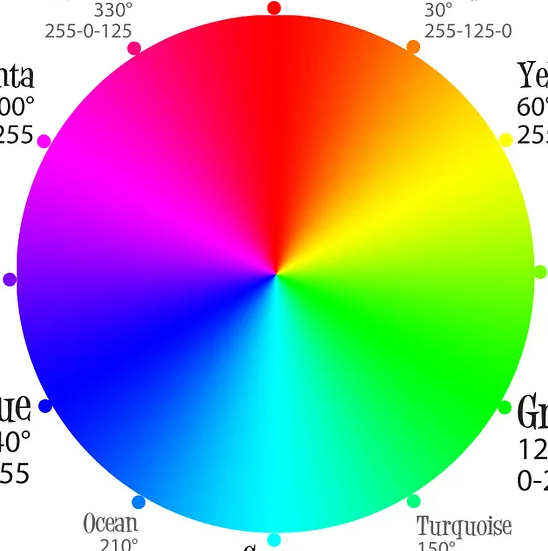
\includegraphics[width=0.5\textwidth]{files/img/unused/teste RGB.png}
% \end{MyCenteredFigure}

% \chapter{Embedding}

ATACHING

% \attachfile{files/codigos/ATTACH.txt}

% test \textattachfile[color=1 0 0]{files/codigos/ATTACH.txt}{Texto 1}

% test \textattachfile[color=0 1 1]{files/codigos/ATTACH.txt}{Texto 2}

% \textattachfile[]{files/codigos/CodigoFonteLaTeX.rar.RemovaEstaPartaParaAcessarOCodigo}{Texto 3}

% EMBEDING

% \embedfile[desc={DECRICAO}]{files/codigos/EMBED.txt}

% \embedfile[desc={DECRICAO2}]{files/codigos/CódigoFonte.rar}

% \embedfile[desc={DECRICAO3}]{files/codigos/CódigoFonte.rar.RemovaEstaPartaParaAcessarOCódigo}

% \embeddedfile{alias}{files/codigos/EMBED2.txt}

% \openfilelink{files/codigos/EMBED2.txt}{Clique aqui para abrir o arquivo}


% \chapter{Easter Egg}

% \begin{MyCenteredFigure}
%   \caption{Teste de Easter Egg}
%   
\includegraphics[width=0.5\textwidth]{files/img/unused/teste}

%   \adjustbox{trim={.25\width} {.25\height} {.25\width} {.25\height},clip}{
\includegraphics[width=0.5\textwidth]{files/img/unused/teste}}
% \end{MyCenteredFigure}

% \chapter{Build}

1

ABCDEFGHIJKLMNOPQRSTUVWXYZ

2


% Ficha catalográfica

% !TEX root = base.tex
% --- Inserir folha de aprovação --- %

% Isto é um exemplo de Folha de aprovação, elemento obrigatório da NBR
% 14724/2011 (seção 4.2.1.3). Você pode utilizar este modelo até a aprovação
% do trabalho. Após isso, substitua todo o conteúdo deste arquivo por uma
% imagem da página assinada pela banca com o comando abaixo:
% \includepdf{folhadeaprovacao_final.pdf}
\begin{folhadeaprovacao}

  \begin{center}
    {\ABNTEXchapterfont\large\imprimirautor}

    \vspace*{\fill}\vspace*{\fill}
    \begin{center}
      \ABNTEXchapterfont\bfseries\Large\imprimirtitulo
    \end{center}
    \vspace*{\fill}

    \hspace{.45\textwidth}
    \begin{minipage}{.5\textwidth}
      \imprimirpreambulo
    \end{minipage}
    \vspace*{\fill}
  \end{center}

  Trabalho aprovado. \imprimirlocal, \DataImpressao :

  % \assinatura{\textbf{Prof. Dr. \imprimirorientador} \\ Orientador}
  \assinatura{\textbf{Prof. Dr. Fermín A. Tang Montané} \\ Orientador}
  \assinatura{\textbf{Prof. Dr. Luis Antonio Rivera Escriba} \\ Membro da banca}
  \assinatura{\textbf{Profa. Dra. Annabell Del Real Tamariz} \\ Membro da banca}
  %\assinatura{\textbf{Professor} \\ Convidado 3}
  %\assinatura{\textbf{Professor} \\ Convidado 4}

  \begin{center}
    \vspace*{0.5cm}
    {\large\imprimirlocal}
    \par
    {\large\DataImpressao}
    \vspace*{1cm}
  \end{center}

\end{folhadeaprovacao}

% \chapter*{Banca}

% Por enquanto, a banca que eu tenho em mente é composta por:

% \begin{enumerate}
%   \item Fermín Alfredo Tang Montané (Orientador)
%   \item Annabell del Real Tamariz (Ex Chefe do Laboratório de Matemática)
%   \item Oscar Alfredo Paz La Torre (Ex Diretor do CCT)
%   \item Luiz Humberto Guillermo Felipe (Chefe do Laboratório de Matemática)
%   \item Márcia Diretora CCT (Diretora do CCT)
% \end{enumerate}

% Conforme resolução 004/2007 do COLAC, artigo 9 e parágrafo 1, a banca examinadora deverá ter a seguinte composição:
% (i) o Professor Orientador e/ou Co-orientador do aluno, que presidirá os trabalhos,
% (ii) um membro indicado, de comum acordo, pelo estudante e seu Professor Orientador ou Co-Orientador e
% (iii) um membro indicado pelo Colegiado do Curso. Em caráter excepcional, um dos três avaliadores poderá ser um Mestre ou doutorando ou pós doutorando que tenha formação compatível com o tema da monografia. Além dos membros titulares, deverá ser indicado um membro suplente. A composição da banca deverá ser aprovada pelo Colegiado do Curso, dando preferência para que o presidente seja doutor. Quando o orientador ou co-orientador estiver impossibilitado de estar presente na banca examinadora, o coordenador do Curso poderá representá-lo, desde que seja requerido por escrito e antecipadamente pelo orientador do aluno.

\begin{dedicatoria}
  \vspace*{\fill}
  \centering
  \noindent

  Dedico este trabalho a todos aqueles que me apoiaram, incentivaram e cobraram pela conclusão do meu TCC. Àqueles que vieram antes de mim, Sânya e Ricardo, que inicialmente pesquisaram e desenvolveram seus trabalhos sobre o mesmo tema. À UENF, ao CCT e ao Curso de Ciência da Computação, que me guiaram na jornada de aprendizado e crescimento acadêmico e que poderão usufruir das semestes que plantei, caso vinguem. Mas principalmente dedico a todos os futuros alunos e pesquisadores, que inconformados com o \textit{status quo}, buscam sempre melhorar a si mesmos e ao mundo ao seu redor.

  \vspace*{\fill}
\end{dedicatoria}
\begin{agradecimentos}

  Agradeço aos meus pais que se dedicaram para que eu pudesse estar cursando esta graduação, assim podendo completar mais uma etapa da minha vida. Sem o apoio, conselhos, carinho e amor, nada disso seria possível. Sou eternamente grato por tudo que vocês fazem e sempre fizeram para que minha vida fosse especial.

  Agradeço aos meus amigos e colegas de curso que compartilharam comigo bons momentos, risadas e refeições no RU. Em especial, aos meus grandes amigos Daniel Brito e José Lucio, que unidos pela Iniciação Científica e pela progressão contínua, seguimos juntos até o fim, também aos meus amigos João Víttor e Adriano, que entraram comigo no curso e que, apesar dos percalços, seguem sendo grandes companhias pra vida.

  Agradeço ao meu orientador, Prof. Dr. Fermín Alfredo Tang Montané, que se dispôs a me ouvir reclamar e propor ideias. Que se dispôs a me orientar mesmo que em suas férias, e que sempre esteve disponível para me ajudar.

\end{agradecimentos}
\begin{epigrafe}
  \vspace*{\fill}
  \begin{flushright}
    \textit{``Quando você não sabe alguma coisa,\\
      procura quem sabe e pergunta.\\
      Pra não fazer feio, nem passar vergonha.''\\
      Vovô Nando, 01/12/2023}
  \end{flushright}
\end{epigrafe}
% resumo em português
\setlength{\absparsep}{18pt} % ajusta o espaçamento dos parágrafos do resumo
\begin{resumo}

  Esta monografia apresenta um estudo sobre a criação de grades horárias em universidades, com foco na Universidade Estadual do Norte Fluminense, e o desenvolvimento de um sistema de suporte à decisão para a criação de grades horárias. Este processo é complexo e envolve diversos fatores, como a disponibilidade de salas e professores, a quantidade de alunos e a demanda por disciplinas. Como uma das maiores dificuldades no ramo acadêmico da criação de grades horárias é a modelagem do problema, este trabalho se propõe a estruturar as informações referentes à instituição estudada através de pesquisas e entrevistas. A partir disso, foi possível identificar a sequência de criação das grades e as restrições impostas pela instituição, podendo assim propor um sistema que auxilie o processe. Para tanto, o sistema foi desenvolvido utilizando JavaScript e a biblioteca React, sendo hospedado no GitHub Pages e utilizando da Amazon Web Services para a execução de seu \textit{backend} e armazenamento de dados. Suas funcionalidades incluem as funcionalidades CRUD (criar, ler, atualizar e deletar) de professores, disciplinas, salas, alunos, turmas e horários, a criação automatizada de uma grade horária inicial para o curso de Ciência da Computação da UENF, a visualização de conflitos dentre os recursos alocados e a análise história dos dados armazenados no sistema.

  \textbf{Palavras-chave}: Criação de Grades Horárias. Agendamento de Aulas Universitárias. Heurísticas. Design de Interação. Interação Humano-computador.

  % Resumo

  % Segundo a ABNT (2003, 3.1-3.2), o resumo deve ressaltar o objetivo, o método, os resultados e as conclusões do documento. A ordem e a extensão destes itens dependem do tipo de resumo (informativo ou indicativo) e do tratamento que cada item recebe no documento original. O resumo deve ser precedido da referência do documento, com exceção do resumo inserido no próprio documento. (. . . ) As palavras-chave devem figurar logo abaixo do resumo, antecedidas da expressão Palavras-chave:, separadas entre si por ponto e finalizadas também por ponto.

  % Palavras-chave: latex. abntex. editoração de texto.

\end{resumo}

% resumo em inglês
\begin{resumo}[Abstract]
  \begin{otherlanguage*}{english}

    This monograph presents a study on the creation of timetables in universities, focusing on the Universidade Estadual do Norte Fluminense, and the development of a decision support system for the creation of timetables. This process is complex and involves several factors, such as the availability of classrooms and teachers, the number of students and the demand for disciplines. As one of the greatest difficulties in the academic field of creating timetables is the modeling of the problem, this work proposes to structure the information regarding the institution studied through research and interviews. From this, it was possible to identify the sequence of creating the timetables and the restrictions imposed by the institution, thus being able to propose a system that assists the process. For this, the system was developed using JavaScript and the React library, being hosted on GitHub Pages and using Amazon Web Services for the execution of its backend and data storage. Its features include the CRUD (create, read, update and delete) functionalities of teachers, disciplines, classrooms, students, classes and schedules, the automated creation of an initial timetable for the Computer Science course at UENF, the visualization of conflicts among the allocated resources and the historical analysis of the data stored in the system.

    \textbf{Keywords}: Timetabling. University Class Scheduling. Heuristics. Interaction Design. Human Computer Interaction.

  \end{otherlanguage*}

  % \vspace{\onelineskip}
  % \noindent

\end{resumo}
\pdfbookmark[0]{\listfigurename}{lof}
\listoffigures*
\cleardoublepage{}
\pdfbookmark[0]{\listtablename}{lot}
\listoftables*
\cleardoublepage{}
% \pdfbookmark[0]{\lstlistlistingname}{lot}
\lstlistoflistings
\cleardoublepage{}
\pdfbookmark[0]{\contentsname}{toc}
\tableofcontents*
\cleardoublepage{}

\textual{} % --- INÍCIO DOS ELEMENTOS TEXTUAIS ---

\chapter{Introdução} \label{chap:introducao}             % ##   1

No ensino superior brasileiro, cada curso de uma instituição de ensino tem em seu projeto pedagógico, ou seja, no documento que rege quais as atribuições e justificativas de existência do curso, uma listagem de disciplinas a serem ministradas em cada semestre ao longo de sua duração esperada. Disciplinas estas que para serem cursadas os discentes precisam cumprir determinados requisitos.

Embora haja o planejamento de duração do curso, diversos fatores podem influenciar a previsão, dentre eles podemos citar eventos como: quebra de pré-requisitos, trancamento de matrícula, transferências, reprovações, indisponibilidade de professores, greves, dentre tantos outros.

Estes eventos tendem a, no geral, aumentar o tempo médio para conclusão do curso. Situação em sua maioria indesejada tanto pelos alunos, que mesmo durante seu estudo já visam o mercado de trabalho, quanto pelos professores e pela instituição, visto que a evasão do ensino superior brasileiro é um problema existente e estudado a fim de ser minimizado.

Com isso, é esperado que a instituição busque alternativas para tornar mais dinâmica e atrativa a experiência dos discentes durante sua jornada. Uma dessas formas é tentando minimizar o impacto que os atrasos na grade causam nos semestres consecutivos. Para isso sendo então necessária uma análise das disciplinas que devem ser oferecidas no próximo semestre, sendo então necessário definir \textbf{quais}, \textbf{quando}, \textbf{onde}, \textbf{por quem} e \textbf{para quem} serão ministradas. Esta tarefa, entretanto, não é trivial.

\section{O problema} \label{sec:Problemáticas}        % ###  1.1

Embora seja um problema atualmente, isso não significa que seja recente. Desde 1978 \cite{Barham1978} o termo \textit{timetabling} encontra-se no meio acadêmico como o termo referente ao construção de grade horária, sendo este o ramo de pesquisa que direciona este trabalho. Neste artigo de 1978 já se propunha uma forma para que se obtivesse um construção otimizada, e demonstrava que o método utilizado gerava bons resultados.

Outra característica deste problema é informada por \citeonline{Thomas2009} que fala sobre a multidimensionalidade do problema de \textit{timetabling}. Por causa dessa questão há uma complexidade elevada para conseguir conceber visual e mentalmente de que forma os dados relacionados ao problema se estruturam, assim dificultando a elaboração de sistemas computacionais que auxiliem nessa tarefa.

Também segundo \citeonline{Miranda2012}, embora o problema de atribuição de salas não seja novo e tenha extensa literatura a seu respeito, são poucos os que de fato implementaram um sistema para suporte de decisões. Isso se dá por diversos fatores, também listado pelo autor fazendo referência a trabalhos anteriores, sendo alguns deles a resistência organizacional a mudanças e adoção de novas tecnologias, nível de dificuldade do problema, dentre outros. Algumas outras características que se apresentam como problemas são a falta de otimalidade das grades horárias desenvolvidas em boa parte das instituições de ensino superior e a quantidade de tempo necessária para a criação dessas grades não-ótimas.

Em se tratando do caso específico da UENF, \textbf{o problema} que será abordado, consiste na criação de grades horárias se apresenta com suas próprias peculiaridades, dentre elas listam-se a aquisição de uma estimativa de alunos que desejam cursar determinada disciplina, a existência de diversas etapas na criação da grade que envolvem diferentes entidades da instituição cada uma delas contando com informações incompletas durante o processo, que vão aos poucos convergindo para uma solução final, que mesmo que não ótima, é uma solução viável. Ainda assim, a quantidade de tempo necessária para a criação de uma grade horária é extensa e não garante a otimalidade da solução encontrada.

Considerando que situações como a descrita acima são passíveis de ocorrer, e que a tarefa de criação de grades horárias é recorrente, um sistema de suporte à decisão que auxilie na centralização dos dados e que auxilie na percepção de alocações inapropriadas se faz necessário.

\section{Hipótese} \label{sec:Hipótese}                  % ###  1.2

Dada as características intrínsecas ao problema de agendamento de grade horária, é esperado que os \textit{softwares} atualmente existentes que lidam com este problema não apresentem completas capacidades de se moldar ao caso de uma instituição específica. E, caso a primeira hipótese se apresente correta, o \textit{software} a ser desenvolvido, assim como seus similares, se apresentará como uma solução plausível para a resolução do problema proposto embora ainda apresente melhorias possíveis a serem implementadas. O \textit{software} se apresentará de tal forma que cada uma das partes interessadas possam utilizá-lo de forma independente, sem se limitar à ausência de informações advindas das outras partes.
% Eu poderia adicionar aqui a hipótese de que a atual criação de grades horárias é falha e ineficiente ou algo mais suave.

\section{Objetivos} \label{sec:Objetivos}                % ###  1.3

Os objetivos desta monografia podem ser divididos entre gerais e específicos, não havendo relação de superioridade de um em relação ao outro, visto que ambos igualmente nortearão o desenvolvimento da pesquisa.

% \subsection{Gerais} \label{ssec:Gerais}                % #### 1.3.1

Como \textbf{objetivos gerais} temos o desenvolvimento de um sistema de suporte à decisão tal que aumente a eficiência, eficácia e efetividade do processo de criação de grades horárias que semestralmente demandam extensa quantidade de tempo dos coordenadores de curso na UENF e não alcançam a otimalidade. Em particular, nesse trabalho, trata-se do caso específico do curso da Ciência da Computação. Nesse processo, também é esperado que as grades horárias finais tragam a satisfação de todos os participantes do processo, desde os coordenadores de curso até os alunos.

% \subsection{Específicos} \label{ssec:EspeEspecíficos}  % #### 1.3.2

Como \textbf{objetivos mais específicos}, podemos listar os seguintes:

\begin{itemize}
  \item Entender de que forma os setores administrativos da UENF lidam com a questão do \textit{timetabling};
  \item Atender às principais necessidades dos responsáveis pela criação de grades horárias;
  \item Modelar o sistema de \textit{timetabling} de acordo com os requisitos demandados;
  \item Incentivar o uso do \textit{software} para a auxiliar na criação da grade horária.
\end{itemize}

\section{Justificativas} \label{sec:Justificativas}      % ###  1.4

% Levando em conta a problemática evidenciada e os sucessos prévios dos artigos anteriores, vê-se grande potencial de auxílio e aumento na satisfação de todos os que utilizarem os métodos propostos.
Não havendo um sistema geral que solucione todos os casos como evidenciado pelos pesquisadores da área, resta aos interessados rumarem em busca de uma solução entalhada nos moldes de sua instituição específica.

No caso específico na UENF, as grades horárias são construídas gradualmente e constantemente trabalham com informações incompletas, o que dificulta a percepção de alocações inapropriadas. Para tanto, sendo assim, faz-se válida a pesquisa e desenvolvimento de um sistema de suporte à decisão que seja capaz de lidar com a ausência de informações e a percepção dos conflitos advindos de alocações indevidas.

\section{Metodologia} \label{sec:Metodologia}            % ###  1.5

Considerando as dificuldades encontradas em trabalhos anteriores, entende-se que o maior desafio será superar as especificidades que serão encontradas durante a modelagem da universidade em questão. Para isso, será inicialmente necessária uma pesquisa bibliográfica com foco no estudo das abordagens qualitativas realizadas anteriormente que obtiveram sucesso em elicitar os requisitos adequados para as instituições de ensino.

Com este conhecimento, um material inicial para a pesquisa exploratória e qualitativa deve ser desenvolvido levando em conta as questões próprias da universidade em questão, visando também coletar dados relevantes para uma futura pesquisa com maior enfoque em características emergentes que a pesquisa anterior pode levantar, similar a como foi proposto e realizado por \citeonline{Andre2018}. Esta pesquisa exploratória sobre a realidade da instituição se subdivide em três frentes: o estudo sobre a \textbf{documentação teórica}, \textbf{entrevista} com os \textit{stakeholders} (gestores envolvidos na elaboração do quadro de horários) e \textbf{formulário} direcionado aos alunos.

% Na \textbf{documentação teórica}, espera-se encontrar informações sobre a estrutura organizacional da UENF, bem como as regras que regem a criação de grades horárias. Quais são os cargos envolvidos e quais são as responsabilidades de cada um deles. Com esta informação, estabelecem-se assim os \textit{stakeholders} iniciais. Na \textbf{entrevista}, algumas informações esperadas giram em torno das percepções dos \textit{stakeholders} do sistema proposto. Estas percepções incluem o entendimento deles quanto ao método atual e às alternativas existentes, nível de insatisfação com o método atual, nível de desejo quanto à um novo método. Além disso, espera-se aproveitar o ensejo para elicitar as características e funcionalidades que gostariam de ter em um sistema de suporte à decisão, solicitando também que deem informações adicionais que gostariam de acrescentar. \textbf{Questionamentos} também serão realizados com alunos, porém em formato de formulário online para atingir mais objetivamente uma quantidade mais vasta de respondentes. Espera-se obter informações sobre a satisfação dos alunos com as grades horárias atuais, para assim poder confirmar se a insatisfação é generalizada e percebida por todos os envolvidos.

Sendo compreendido então o cenário atual da universidade, será então necessário modelar o sistema de suporte à decisão de acordo com as especificidades encontradas, compilando, de maneira geral, os estágios do Design de Interação, o funcionamento do sistema, o diagrama conceitual do seu banco de dados, e suas principais diferenças em relação aos trabalhos anteriores.

Por fim, será apresentado o processo do desenvolvimento do sistema, partindo dos projetos anteriores que motivaram a execução deste trabalho, a tentativa de acesso aos dados acadêmicos da instituição, a prototipação do sistema, e o desenvolvimento do sistema em si, que foi subdividido em três diferentes versões, encerrando com mais detalhes sobre as duas características mais notáveis deste sistema: a resolução dos conflitos percebidos e a criação automatizada de uma grade horária inicial.

% DAR MAIS ENFOQUE A TUDO O QUE FOI USADO

\section{Organização} \label{sec:Organização}            % ###  1.6

Este trabalho abordará capítulos que tratam dos seguintes tópicos:

\begin{itemize}
  % \item O \autoref{chap:introducao} de introdução traça informações gerais sobre o assunto do trabalho, elaborando mais detalhadamente quanto à sua \hyperref[sec:Problemáticas]{problemática}, \hyperref[sec:Hipótese]{hipótese}, \hyperref[sec:Objetivos]{objetivos}, \hyperref[sec:Justificativas]{justificativas}, a \hyperref[sec:Metodologia]{metodologia escolhida} e a \hyperref[sec:Organização]{organização de suas informações};
  \item O \autoref{chap:marco} de revisão literária informa mais detalhadamente sobre os problemas de agendamento, suas categorias, soluções, desafios e definições de termos;
  \item O \autoref{chap:modelagem} de modelagem, apresenta-se a conceitualização macro de como o sistema deve se comportar, quais são as suas funcionalidades e quais são os seus objetivos;
  \item O \autoref{chap:instituicao} de contexto da instituição apresenta a \hyperref[sec:estatuto]{Universidade Estadual do Norte Fluminense Darcy Ribeiro (UENF), suas características, estrutura organizacional}, \hyperref[sec:entrevistas]{entrevistas com os \textit{stakeholders} relacionados à criação de grades horárias} e a \hyperref[sec:sequencia]{sequência de passos para a criação de uma grade horária};
  \item O \autoref{chap:desenvolvimento} de desenvolvimento, pode ser visto o processo de criação do sistema, contextualizado a partir dos projetos anteriores, passando pela prototipação, para então chegar ao desenvolvimento em três etapas do sistema final;
        % \item O \autoref{chap:experimentos} de experimentos apresenta a validação do sistema desenvolvido através de testes de criação de grade horária seguido de resolução dos conflitos encontrados;
  \item O \autoref{chap:resultados} de resultados demonstra as páginas do sistema desenvolvido, as funcionalidades implementadas e outras ferramentas disponíveis para a gestão dos horários;
  \item O \autoref{chap:conclusoes} finaliza o presente trabalho apresentando as conclusões indicando caminhos a serem seguidos por pesquisadores posteriormente.
        % \item O \autoref{chap:apendice} de apêndices apresenta informações adicionais que não se encaixam nos capítulos anteriores, mas que são relevantes para o entendimento do trabalho, sendo eles o código-fonte do sistema e da elaboração desse texto, a pesquisa realizada e a análise de seus resultados.
\end{itemize}

\chapter{Marco teórico} \label{chap:marco}                                                              % ##   2.

Antes de prosseguirmos com o desenrolar deste trabalho, é adequado que primeiro definamos alguns conceitos para o melhor entendimento do trabalho como um todo. Iniciaremos com a definição do \hyperref[sec:termos]{Problema de \textit{timetabling}}, suas subdivisões, \hyperref[ssec:desafios]{suas complexidades} e \hyperref[ssec:erros]{possíveis errosna gestão das informações}. Em seguida, abordaremos os \hyperref[sec:resolucao]{métodos de resolução} para o problema, nos baseando em compilados de informações sobre os trabalhos anteriores. Especifica-se também como que se dá o \hyperref[sec:anteriores]{Problema de \textit{Timetabling na UENF (PTT-UENF)}}, com base nos trabalhos anteriores. Por fim, são apresentadas diversas \hyperref[sec:teorias]{estratégias de solução baseadas na otimização}, que serão utilizadas conceitualmente durante o desenvolvimento deste trabalho.

% O Problema de Programação de Horários (Timetabling Problem) é um problema de grande relevância e amplamente estudado na área de Pesquisa Operacional. Um número significativo de trabalhos sobre esse problema foi publicado nos últimos anos e conferências regulares discutem o tema no meio científico [Splinder2010].
% Sânya
% O Problema de Programação de Horário Escolar pode ser generalizado como o escalonamento semanal das aulas em uma escola sem que professores e alunos tenham mais de uma aula ao mesmo tempo (estudantes são agrupados em turmas com os mesmos planos de aula). Já o Problema de Programação de Horário de Disciplinas em Universidades como o escalonamento semestral das aulas de um conjunto de disciplinas de uma universidade de modo a evitar colisão de horários (estudantes geralmente são considerados individualmente) [Paim__2010].
% Sânya

% Existem algumas ferramentas comerciais que prometem a geração automatizada de grades de horários, entretanto, sua utilização é pouco frequente uma vez que este tipo de problema incorre em necessidades específicas de um determinado curso, em detrimento das soluções genéricas existentes
% F. Vieira & H. Macedo, Scientia Plena 7, 039901 (2011) 

% O school timetabling possui uma quantidade de recursos menor, pois uma turma já possui uma sala especificada e seu grupo de alunos, em sua maioria, é predeterminado, o que faz com que a complexidade seja reduzida. Em problemas de course timetabling existe um grande conjunto de restrições: disciplinas de uma mesma turma podem ser alocadas em salas diferentes, cada disciplina é constituída por alunos de diversos cursos, professores possuem restrições de horário por desempenharem outras atividades na instituição, cada disciplina possui conjuntos de pré-requisitos que devem ser respeitados, entre outras.
% F. Vieira & H. Macedo, Scientia Plena 7, 039901 (2011) 

\section{Problema de \textit{timetabling}} \label{sec:termos}                                                        % ###  2.1

% Ao longo dos anos de desenvolvimento acadêmico, diversos assuntos vão se aprofundando e se tornando mais específicos, assim, os estudiosos acabam cunhando novos termos que o auxiliam a desvencilhar as novas áreas específicas das suas áreas originárias. Porém, existe o potencial de que haja um crescimento desestruturado destes novos termos, assim vários termos diferentes podem se referir a um mesmo conceito, enquanto que um mesmo termo pode se referir a vários conceitos diferentes de acordo com o autor.

Segundo \citeonline{Wren1996}, \textit{timetable} é definido como uma estrutura que mostra quando eventos ocorrerão, não havendo necessariamente a alocação de recursos. Vale ressaltar que este termo não tem seu uso limitado para os fins desta pesquisa, sendo também usado para problemas de alocação de enfermeiros, esportes, funcionários e transportes \cite{Arratia2021}. Entretanto, neste trabalho, abordaremos principalmente os termos relacionados ao que pode ser chamado de \textit{Educational Timetabling} (Ed-TT) \cite{Alencar2019}, que é o que tende a envolver um conjunto específico de recursos relacionados à educação.

\citeonline{Wren1996} também define os conceitos para \textit{class timetable}, \textit{university examination timetable} e \textit{university class timetable}, tendo relevância apenas o último, que considera a disponibilidade de professores e salas, a quantidade de alunos e os requisitos que determinada disciplina exige.

Assim como feito por \citeonline{Wren1996}, definiremos os conceitos dos termos que serão usados ao longo deste trabalho. Sendo assim, usaremos a definição do termo \textit{university class timetable} de forma simplificada, sendo chamada apenas de \textit{timetable}, ``grade horária'' ou ``tabela horária''.

% Sânya fala sobre International Timetabling Competition

Aqui, visto que uma solução final envolverá várias dimensões (Professores $\times$ Disciplinas $\times$ Sala $\times$ Alunos $\times$ Horários $\times$ Dias), consideraremos \textit{timetable} como esse pacote de valores distribuídos em uma só estrutura. Para que esses valores sejam distribuídos, daremos o nome de \textbf{alocação} ao ato de criar qualquer relação entre as dimensões. Como a relação de horários e dias será considerada fixa, a \textbf{alocação} se referirá à atribuição como a de professores a disciplinas, disciplinas a salas, disciplinas a um determinado padrão de dias e horários, etc.

Para que esta alocação ocorra, é necessário atender a certos critérios, e aí entra o ``problema de organização de grade horária'', também chamado de \textit{timetabling problem}. Esta é uma subcategoria do \textbf{problema de otimização de agendamento} (\textit{scheduling Optimization Problem}) \cite{Alencar2019} que por sua vez é definido por \citeonline{Wren1996} como sendo:

\begin{quote}\footnotesize
  Resolver problemas práticos relacionados à alocação, sujeito a restrições, de recursos a objetos sendo colocados no espaço-tempo, usando ou desenvolvendo quaisquer ferramentas que possam ser apropriadas. Os problemas irão frequentemente se relacionar à satisfação de certos objetivos. \cite{Wren1996}
\end{quote}

Outro termo relevante a se pontuar são as \textit{hard and soft constraints} que podemos chamar de restrições rígidas e flexíveis. \citeonline{Alencar2019} as definem dizendo que as restrições rígidas são de atendimento obrigatório para que a solução seja considerada viável, enquanto as restrições flexíveis são opcionais, mas convenientes para melhorar a qualidade da solução obtida.

Ambos os tipos de restrições são importantes para a resolução do problema, e são altamente dependentes do contexto em que estão inseridas. Em determinada instituição de ensino. Por exemplo: uma restrição rígida onde uma disciplina não possa durar mais do que três horas pode ser considerada flexível em outra instituição. Sendo então, também dependente do contexto de cada instituição a definição das regras de viabilidade e inviabilidade de soluções.

Em seu trabalho, \citeonline{Souza2000} distingue entre viabilidade e otimalidade. Para ele, no primeiro caso, a solução do problema consiste basicamente em encontrar um conjunto de alocações tal que satisfaça a todas as restrições impostas. Já no segundo caso, após encontrar-se diversas soluções viáveis, busca-se dentre elas aquelas que melhor atendam às soluções flexíveis baseado em critérios de avaliação de uma função objetivo. \citeonline{Dunke2023} comentam que há algoritmos que consideram as restrições rígidas e flexíveis de forma simultânea, enquanto outros resolvem primeiro as restrições rígidas e depois as flexíveis.

Alguns outros termos similares a este campo de pesquisa encontrados na literatura são \textit{periodic event scheduling problem}, \textit{timetable scheduling}, \textit{class scheduling}, \textit{student scheduling}, \textit{university course timetabling}, dentre outros.

\subsection{Questões sobre a complexidade do problema} \label{ssec:desafios}                                                      % ###  2.3

% Apesar da vasta quantidade de trabalhos realizados na área do \textit{Timetabling Problem} segue sendo estudado como devida.

\citeonline{Murray2007} trazem a questão da modelagem como um dos maiores obstáculos. À medida em que a complexidade aumenta, se torna cada vez mais difícil desenvolver uma solução efetiva. Assim fazendo com que a solução para uma universidade possa não ter utilidade para outras, ou até mesmo não seja capaz de lidar com todos os problemas de uma mesma universidade.

Apesar do contrafluxo encontrado na resolução desse problema, \citeonline{Murray2007} citam que, apesar da complexidade, é sim possível desenvolver soluções que tenham uso prático, mesmo que não seja um processo fácil. As ferramentas existem e estão disponíveis. Restando então considerar e resolver as preocupações dos usuários às questões, visto que as técnicas de resolução já se encontram vastamente documentadas.

Com isso, entramos também no ramo da Interação Homem-Máquina, ramo abordado por \citeonline{Andre2018} que visaram em seu desenvolvimento a criação de uma interface focada no usuário. Assim minimizando o atrito na abordagem desse problema complexo. Também sendo área de enfoque de \citeonline{Alencar2019} em sua revisão literária

\subsection{Possíveis erros na gestão das informações} \label{ssec:erros}                                                    % ###  2.5

Dada a grande quantidade de variáveis interconectadas e as características específicas de cada instituição \cite{Miranda2012}, a organização destas informações buscando a melhor solução possível apresenta-se como um desafio. Principalmente se considerarmos que esta solução é, muitas vezes, procurada manualmente, estando também passível de erros humanos como ilustram a \autoref{fig:Academico} e \autoref{fig:CCT}.

\begin{MyCenteredFigure} \caption{Disciplina atribuída no sistema acadêmico à determinada hora e local} \label{fig:Academico}
  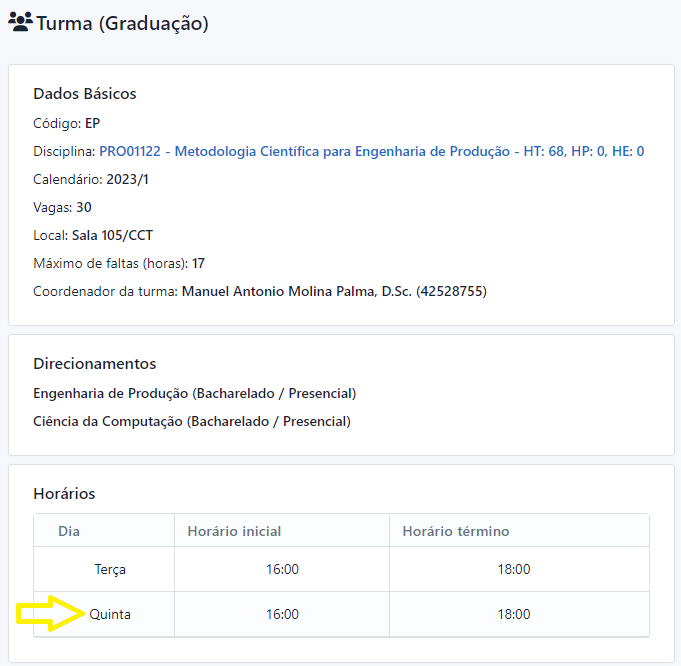
\includegraphics[width=0.8\textwidth]{files/img/2.02!2-marco/Metodologia-Quinta}
\end{MyCenteredFigure}

\begin{MyCenteredFigure} \caption{Falha de alocação na grade horária do CCT de 2023.1} \label{fig:CCT}
  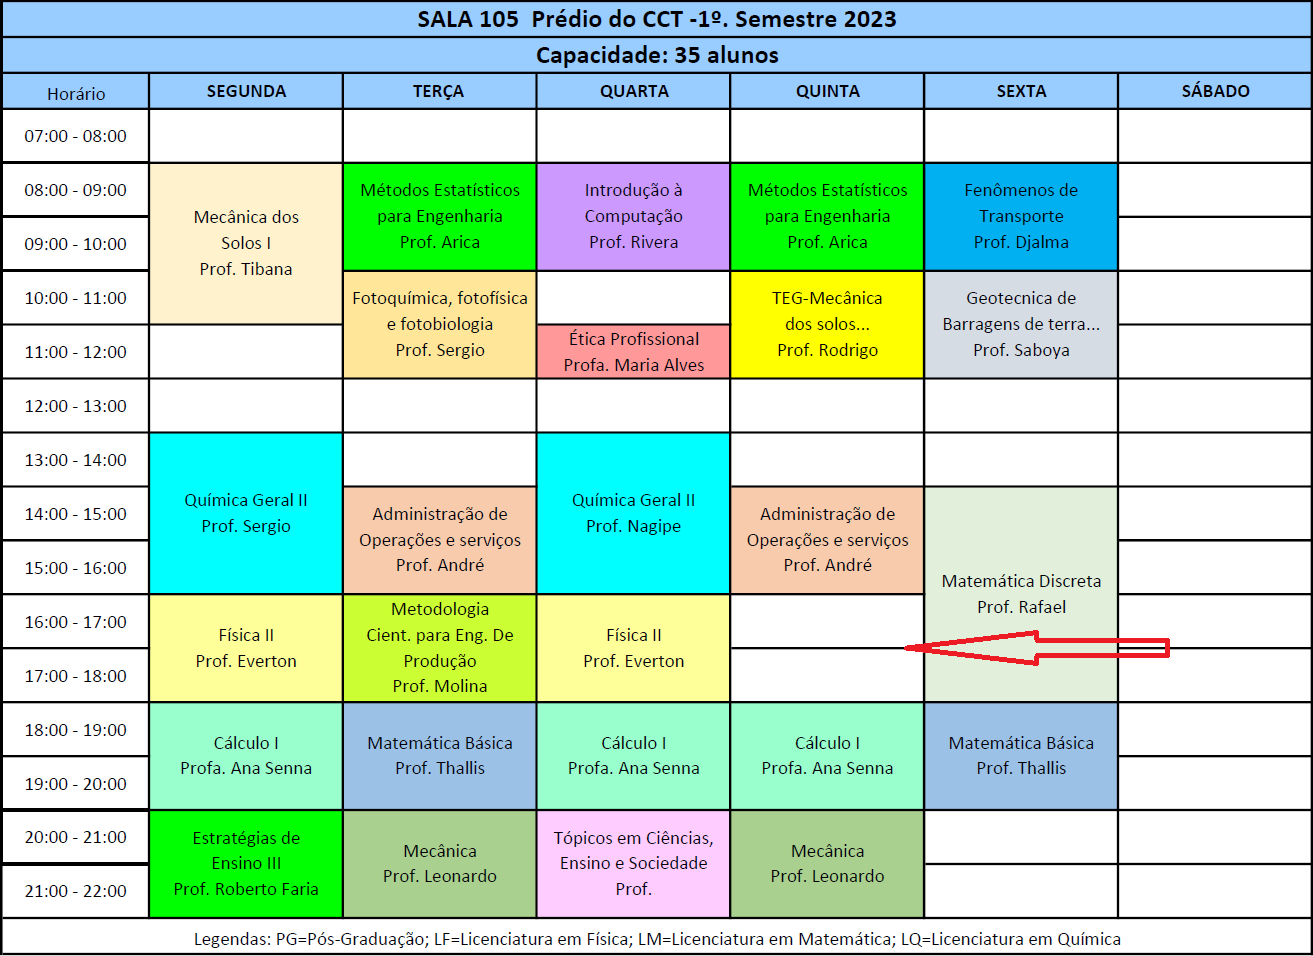
\includegraphics[width=0.8\textwidth]{files/img/2.02!2-marco/Aulas-CCT-105-2023_1}
\end{MyCenteredFigure}

Nestas imagens, fica exemplificado um dos possíveis problemas que podem ocorrer durante a criação de grades horárias, devido à falta de integração das informações em um sistema único. Situação essa que ocorre quando uma seção da universidade (o Sistema Acadêmico, ilustrado pela \autoref{fig:Academico}) aloca uma turma a uma determinada sala, outra seção da mesma instituição (o Centro de Ciência e Tecnologia (CCT), ilustrado pela \autoref{fig:CCT}) pode não estar ciente do mesmo, ou, mesmo estando ciente, pode acabar não delimitando aquela lacuna de tempo como ocupada, assim estando passível de uma segunda alocação naquele período de tempo naquela sala, assim gerando problemas.

\section{Métodos de resolução para o problema de \textit{timetabling}} \label{sec:resolucao}                                                    % ###  2.2

% - O problema de timetabling  a
%  - Origem                    a
%  - Repartições               a
%  - Escopo maior              a
%    - Scheduling              a
%  - Escopo menor              a
%    - Exam                    a
%    - Class                   a
% - TT
%  - Soluções
%  - Desafios
%  - Diversas formas de resolução
%    - Graph Coloring
%    - Heurísticas
%    - Metaheurísticas
%    - IA
%    - etc.
% - Visualização de informações
%  - Benefícios
%  - Motivações
%  - Relação com timetabling
% - Problema geral a ser resolvido
%  - Multi dimensionalidade
%    - Professores
%    - Alunos
%    - Salas
%    - Departamentos
%      - Preferências
%      - Concorrências
%  - Otimalidade
%  - Erros humanos
%  - Número de possibilidades
%  - Interface intuitiva e relevante é um desafio com poucos estudos nos últimos anos
% - Problemas específicos
%  - Regras específicas
%  - Prioridades diferentes
%  - estrutura organizacional semi-exclusiva

% Pesquisar posteriormente sobre imagens que ilustrem bem as diferentes sub categorias de scheduling

Existem diversas implementações já realizadas, utilizando uma miríade de métodos. Em seu trabalho, \citeonline{Miranda2012} informam sobre diversos sistemas baseados em computador para auxiliar na tarefa de agendamento. \citeonline{Miranda2012} também citam dois possíveis métodos de resolução, sendo eles o \textbf{modelo de programação inteira} e os \textbf{métodos heurísticos}.

Dada a variedade de publicações acadêmicas nessa área de estudo, alguns trabalhos buscaram condensar em forma de tabela as informações encontradas. A seguir, algumas das tabelas mais relevantes encontradas durante o estudo bibliográfico serão apresentadas em conjunto com uma breve descrição e análise sobre seu conteúdo.

Na \autoref{fig:Desenvolvimento}, \citeonline{Poulsen2012} traçam a relação entre os diversos autores, ano de sua publicação e seu país de origem com os dados encontrados em seus trabalhos quanto aos parâmetros utilizados na elaboração da grade horária, quão grandes eram cada um de seus parâmetros, quanto tempo foi necessário para achar uma solução e quais foram as técnicas utilizadas.

% Entender o que está dando errado aqui depois

\begin{CenteredFigure} \caption{Resumo de trabalhos, parâmetros, dimensões, tempo e técnicas.} \label{fig:Desenvolvimento}
  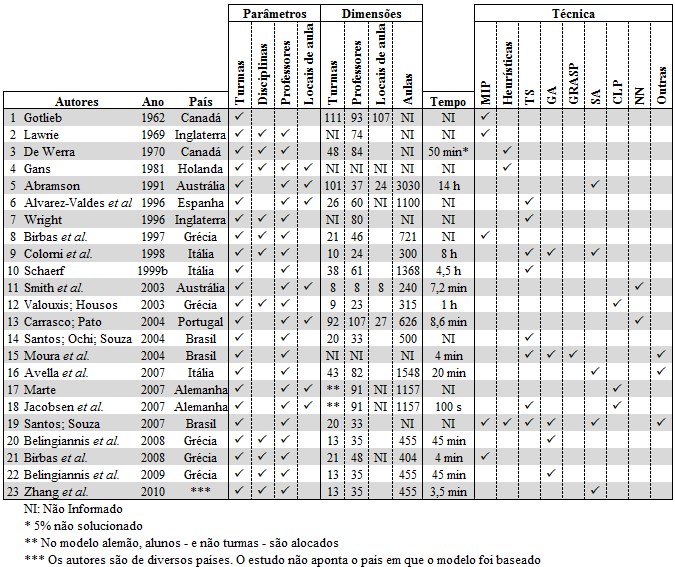
\includegraphics[width=\textwidth]{files/img/2.02!2-marco/Desenvolvimento}
  \legend{Fonte: \citeonline{Poulsen2012}}
\end{CenteredFigure}    % Desenvolvimento

Na \autoref{fig:University}, \citeonline{Arratia2021}, apresentam uma comparação similar à anterior, porém não separada em categorias, apenas categorizando entre verdadeiro e falso algumas características como alocação de salas, professores, nível institucional e método de solução exato ou aproximado.

\begin{CenteredFigure} \caption{Comparação entre artigos que solucionam o problema de grade horária} \label{fig:University}
  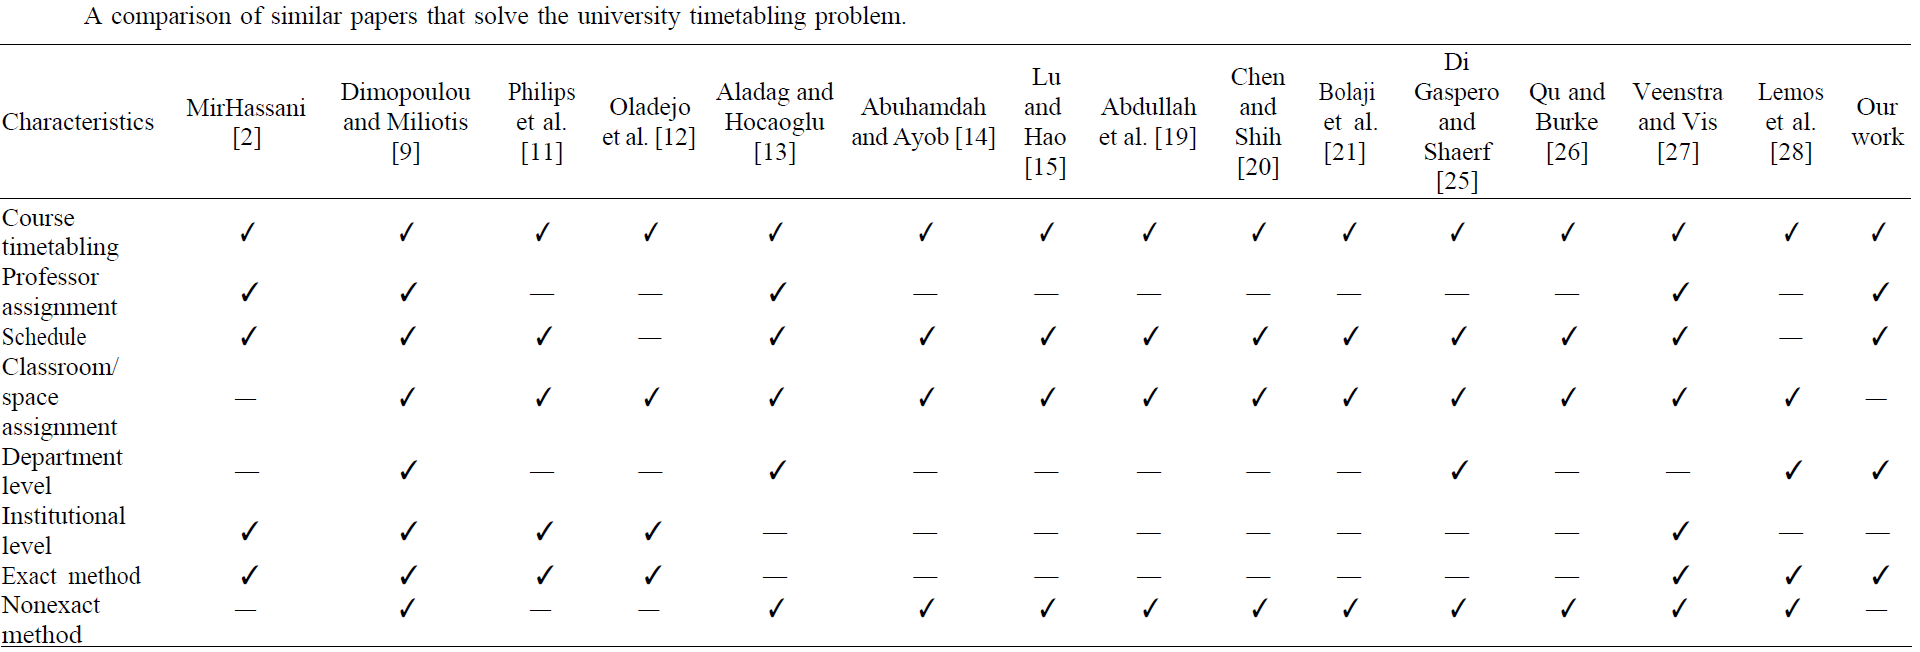
\includegraphics[width=\textwidth]{files/img/2.02!2-marco/University}
  \legend{Fonte: \citeonline{Arratia2021} - editado}
\end{CenteredFigure}    % University

Na \autoref{fig:Visualization}, \citeonline{Alencar2019} exploram uma categoria mais específica do problema, que é a característica da interatividade das interfaces desenvolvidas. Este apresenta características qualitativas quanto aos métodos, os dados dispostos, as técnicas de interação e o método utilizado para solucionar o problema de grade horária educacional. Nesta figura, os autores usam ``Y'' para simbolizar ``Sim'', ``N'' para ``Não'' e ``-'' para ``Inconclusivo''.

\begin{CenteredFigure} \caption{Análise de publicações aceitas} \label{fig:Visualization}
  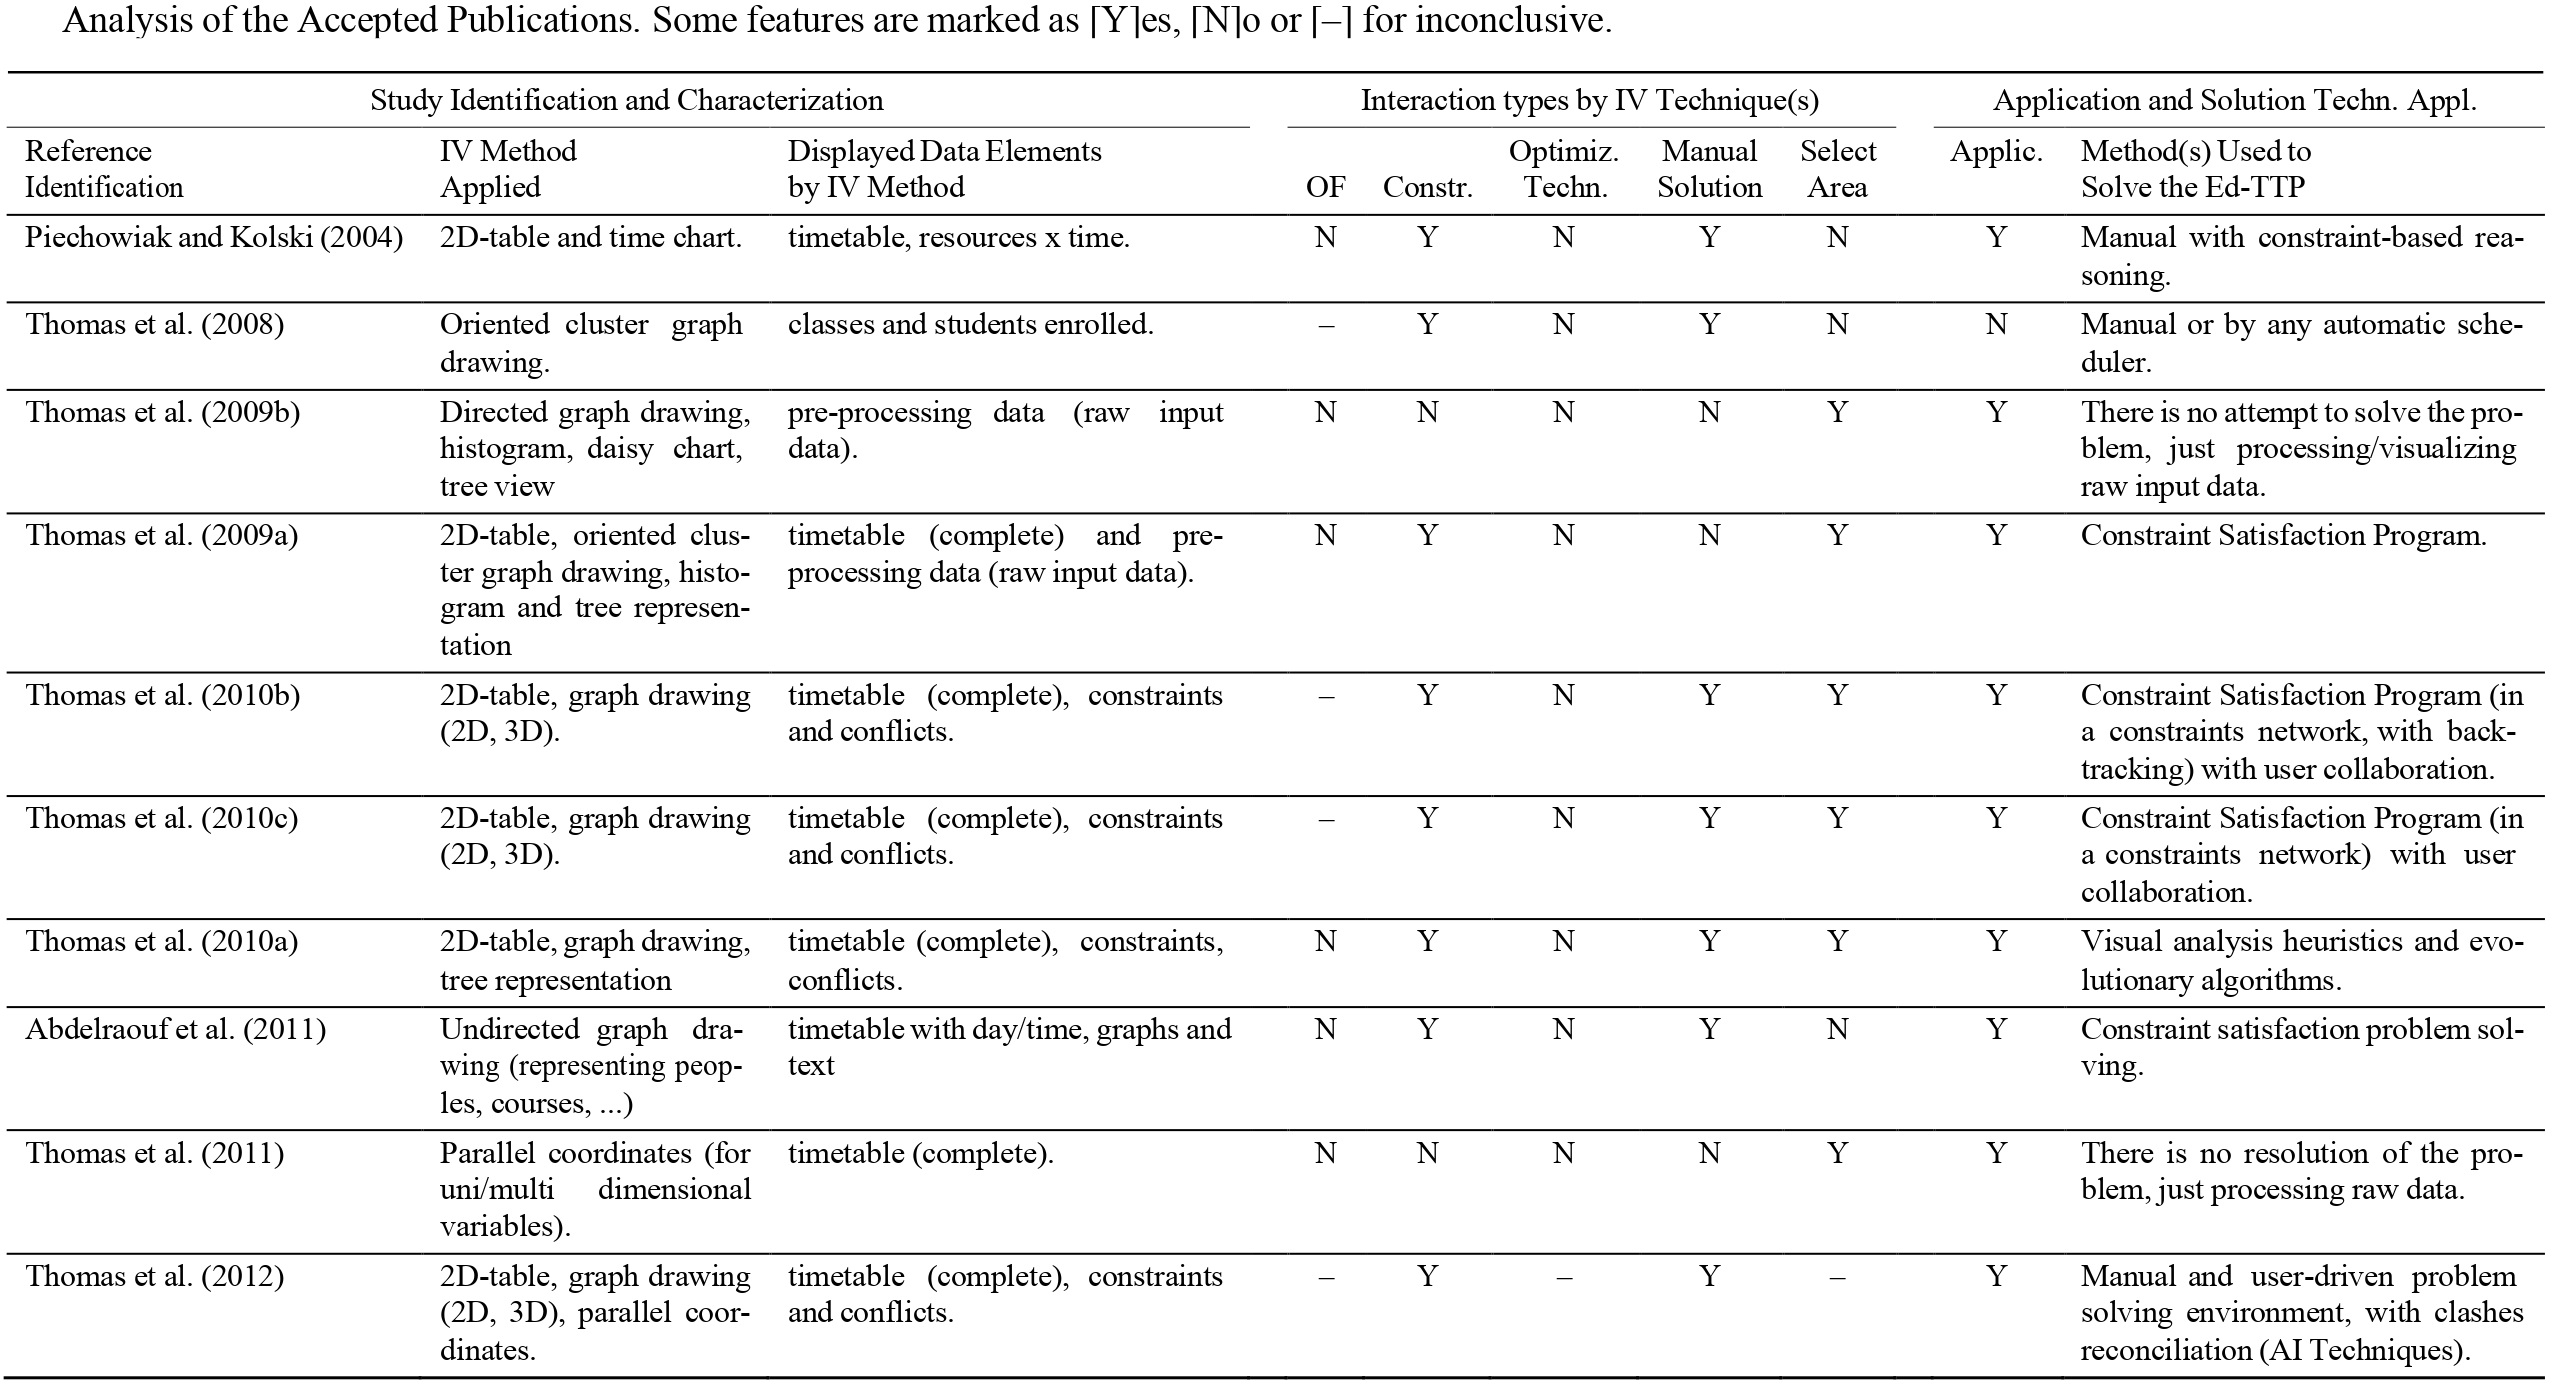
\includegraphics[width=\textwidth]{files/img/2.02!2-marco/Visualization}
  \legend{Fonte: \citeonline{Alencar2019} - editado}
\end{CenteredFigure}    % Visualization

\section{Problema de \textit{timetabling} na UENF (PTT-UENF)} \label{sec:anteriores}                               % ###  2.4

Como visto nas seções anteriores, cada instituição de ensino possui suas próprias características e particularidades. E para a UENF não é diferente. O PTT-UENF apresenta características que tornam o seu problema único, e que, portanto, necessita de uma solução específica. A instituição não se mostra desprovida de histórico na tentativa de resolução deste problema. \hyperref[ssec:sanya]{Sânya} e \hyperref[ssec:ricardo]{Ricardo}, ambos estudantes de Ciência da Computação na UENF, já realizaram trabalhos com o mesmo fim, porém com abordagens diferentes da atual proposta. Em seus trabalhos, \citeonline{SanyaSantos2013} e \citeonline{RicardoSilveira2014} abordaram a criação de tabelas horárias através de métodos de otimização, utilizando heurísticas e metaheurísticas para este fim. A seguir são descritos seus trabalhos anteriores e suas respectivas abordagens.

\subsection{Heurística construtiva para o PTT-UENF} \label{ssec:sanya}     % #### 2.4.1

Em seu trabalho, \citeonline{SanyaSantos2013} aborda o problema de Programação de Horários de Disciplinas em Universidades, tendo como foco o curso de Ciência da Computação da UENF. Sua abordagem foi a de desenvolver um software que fosse capaz de gerar uma grade horária ótima para o curso, levando em conta as restrições impostas pelo curso. Para isso, são explicados diversos métodos possíveis para se alcançar a solução desejada, passando inicialmente pelos métodos construtivos, seguido de métodos refinamento, podendo essas heurísticas serem utilizadas em conjunto com metaheurísticas. \citeonline{SanyaSantos2013} diz que ``as heurísticas são métodos aproximados que se preocupam em encontrar soluções próximas da otimalidade em um tempo computacional hábil''.

Por fim, utilizou uma heurística que consistia em respeitar uma matriz de preferência para a distribuição das disciplinas. Seguindo com o uso do \textit{Simulated Annealing} para a otimização da solução inicial.

\subsection{Metaheurísticas para o PTT-UENF} \label{ssec:ricardo}   % #### 2.4.2

Em seu trabalho, \citeonline{RicardoSilveira2014} aborda também o Problema de Programação de Horários (PPH) em instituições de ensino superior. Ele explora os diversos métodos heurísticos para resolução deste problema que visa encontrar a alocação ótima dos horários em suas grades. Ele teve como objetivo de seu trabalho a implementação de um software que fosse capaz de resolver o PPH do curso de Ciência da Computação da UENF, utilizando os métodos heurísticos Construção Gulosa e Busca Local e os métodos metaheurísticos \textit{Simulated Annealing} e Busca Tabu. Para este fim, ele utilizou a linguagem de programação C para a implementação dos métodos e a linguagem de programação Java para a implementação da interface gráfica do software. Com isso conseguiu elaborar uma ferramenta automatizada para a geração de quadros de horários, alocando aulas e professores em dias e horários disponíveis na semana.

Ele descreve também como possibilidade de trabalho futuro o aperfeiçoamento do banco de dados da ferramenta desenvolvida para que se possa armazenar mais informações pertinentes ao problema, para que o usuário possa realizar modificações no quadro de horários, sendo guiado pelo retorno do Software que informa a viabilidade da alteração, assim gerando maior flexibilidade à aplicação.

\begin{comment} % ``Não cabe muito a crítica aos TCCs anteriores não terem sido implementados''
\subsection{Modelos anteriores} \label{ssec:divergencias}           % #### 2.4.3

Ambos os trabalhos têm sido de grande valia ao rumarem na direção de uma solução para este amplo e complexo problema, percebe-se que o problema que buscaram solucionar ainda se encontra em aberto. Não tendo suas ferramentas alçado voos altos o suficiente para que se tornassem soluções definitivas para o problema no contexto da UENF.

\subsubsection*{\textbf{Sânya}} \label{sssec:sanya} % ##### 2.4.1.1

É dito por \citeonline{SanyaSantos2013} que ``[...] Como na UENF a tarefa de distribuição de sala não varia muito a cada período, sendo feito separadamente por cada centro [...]''. Embora possamos entender o conceito de ``variar muito'' como subjetivo, considerando que mesmo ao longo de um mesmo semestre existem realocações de salas e professores dentro do contexto de um mesmo Centro, podemos entender que a realidade da UENF é de fato muito dinâmica, não se encaixando completamente na solução de alocação única inicial de salas e professores.

Pode-se alegar que tratar da variabilidade de alocações de salas de um mesmo Centro foge do escopo do trabalho, porém, para que o coordenador da Computação tenha fácil acesso aos dados de alocação de salas disponíveis, faz-se necessário que seu uso esteja compartilhado com o Diretor do Centro de Ciência e Tecnologia (CCT), visto que este é o responsável pela alocação de salas de todos os cursos do CCT.

Em outro segmento ela diz que ``[...] as aulas que necessitam de salas com recursos especiais são geralmente já preestabelecidas, não há necessidade de automatizar esta tarefa de distribuição de salas'', mas a realidade é que embora algumas disciplinas tenham suas salas pré-estabelecidas, não são todas as disciplinas que possuem esta característica, isso não significa necessariamente que esta alocação é a mais adequada para a mesma. Então, todas as salas, mesmo que inicialmente pré-estabelecidas, devem estar passíveis de mudanças, mas com possibilidade de se fixar.

Ela diz também que ``Outra tarefa que no presente cenário do curso de Ciência da Computação não viabiliza algum tipo de automatização é a distribuição de professores, pois além de um número muito pequeno destes, não há muitas alternativas de mudanças de suas respectivas disciplinas.''

Quanto à distribuição de professores, a realidade do curso de Ciência da Computação segue a mesma da que foi apontada por \citeonline{SanyaSantos2013}. Entretanto, cada professor tem sua própria gama de disciplinas que se dispõe a ministrar, e a coordenação tende a distribuí-los de acordo com sua preferência. Entretanto, como a demanda dos alunos não se mostra linear como foi estudado, é possível que a distribuição de professores seja feita de forma mais eficiente, considerando a demanda dos alunos, ainda que não se descartem suas preferências pessoais.

Sânya apresenta em seu trabalho uma série de requisitos essenciais e não essenciais para a resolução do problema. Porém, alguns deles não se mostram condizentes com a realidade da universidade. São eles:

\begin{quote}\footnotesize
  \begin{itemize}
    \item Requisitos essenciais, ou seja, obrigatórios:
          \begin{itemize}
            \item \textbf{RE1} - Um professor não pode lecionar aula em duas turmas diferentes no mesmo horário.
            \item \textbf{RE2} - Uma turma não pode ter aula em duas disciplinas no mesmo horário.
          \end{itemize}
    \item Requisitos não essenciais, de qualidade:
          \begin{itemize}
            \item \textbf{RNE1} - O ideal é que existam no máximo duas aulas consecutivas da mesma disciplina.
            \item \textbf{RNE2} - Não devem haver mais de duas aulas da mesma disciplina em um dia.
            \item \textbf{RNE3} - Não preencher os horários de 12h às 14h, pois se trata de horário de almoço.
            \item \textbf{RNE4} - Os professores associados, por terem exclusividade com a instituição, preferem espalhar os horários das aulas dadas, e não acumular todas no mesmo dia.
            \item \textbf{RNE5} - Os professores contratados, por outro lado, preferem que suas aulas sejam alocadas num mesmo dia, ou no menor número de dias possíveis.
          \end{itemize}
  \end{itemize}
\end{quote}

Quanto à citada RE2, a limitação deveria ser mais criteriosa, e se tratando de um requisito não essencial, pois, o conceito de turma é dado pela junção de estudantes que cursam a mesma disciplina, ministrada por um mesmo professor, em um mesmo semestre. Mas em seu trabalho, Sânya considera o conceito de turma como sendo o conjunto de estudantes que ingressaram em um mesmo ano, independente da consideração da existência de repetentes e de suas escolhas pessoais de inscrição.

\textbf{RNE1}, \textbf{RNE2} e \textbf{RNE3}: todas elas não consideram a existência de disciplinas que necessitam de um total de cinco tempos de aula semanais, sendo elas regularmente divididas em dois períodos, um de duas horas e outro de três horas. Que, em situações de necessidades, como é visto na entrevista com o diretor do CCT, acaba sim sendo necessário que se aloque em período de almoço.

\textbf{RNE4} e \textbf{RNE5}: embora estejam direcionadas corretamente, ainda assim não engloba casos de preferência pessoal de cada um dos professores citados. Como por exemplo a possibilidade de não se ministrar aulas em determinados dias da semana por motivos religiosos, seja por parte do quadro permanente, quanto de professores associados.

Outra considerável divergência entre o modelo e a realidade é a definição de que a cada semestre contém apenas 5 turmas de computação. Sendo estas compostas pelos estudantes ingressantes de 5 anos consecutivos, caso este que não se aplica à realidade da universidade, visto que a quantidade de turmas varia de acordo com a demanda semestral, que não necessariamente condiz com todos os estudantes ingressantes de um mesmo ano.

Por fim, Sânya não considera a possibilidade de alocação de professores em mais de uma disciplina, o que é uma realidade na universidade, visto que alguns professores ministram aulas em mais de um curso, e em mais de uma disciplina.

\subsubsection*{\textbf{Ricardo}} \label{sssec:ricardo} % ##### 2.4.1.2

\citeonline{RicardoSilveira2014}, em seu trabalho, apresenta alguns conceitos que se mostraram limitantes em sua modelagem conceitual do problema na UENF. Em sua monografia, ele aborda as turmas como sendo compostas por alunos que ingressaram no mesmo ano, independente de suas escolhas, da demanda, e de possíveis defasagens na progressão do curso. O que não se mostra condizente com a realidade da universidade atualmente, então, mesmo que em 2014, quando o trabalho foi realizado, a realidade fosse esta, não se mostra condizente com a realidade atual, havendo então a necessidade de uma reformulação conceitual.

Ele, assim com \citeonline{SanyaSantos2013}, também não considera a possibilidade de alocação de professores em mais de uma disciplina, múltiplas turmas de uma mesma disciplina, assim como não lida com a distribuição das salas. Ele também considera algumas disciplinas estão fixas, mesmo que pudessem sim ser modificadas por seu responsável, o Diretor do CCT.

Por fim, podemos citar um outro ponto que é a busca pela eficiência e baixo custo de tempo dos métodos utilizados. O que se mostra como ponto positivo, entretanto, mesmo com tamanha eficiência ainda peca em atingir a praticabilidade da solução.

\subsubsection*{\textbf{Parecer geral das divergências}} \label{sssec:divergencias} % ##### 2.4.1.3

O entendimento das falhas passadas em se encontrar uma solução prática ao problema de Programação de Horários da UENF é de suma importância para que se possa evitar que os mesmos erros sejam cometidos novamente. Assim, é necessário que se tenha em mente que a realidade da universidade é dinâmica, e que a solução deve ser capaz de se adaptar a esta dinamicidade.

Vale-se também relembrar o que é dito por \citeonline{Murray2007} que citam em seu trabalho justamente sobre a complexidade presente na modelagem do problema.
\end{comment}

\subsection{Grade horária do curso de Engenharia Civil da UENF} \label{ssec:leciv}                        % #### 2.4.3

Através de pesquisas no \LinkToURL{\LinkSiteUENF}{site oficial da UENF}, mais especificamente na página de horários do LECIV para 2017.2 e 2018.2 foram encontrados alguns PDFs que continha a grade horária do curso de Engenharia Civil para o período de 2017 e 2018. A \autoref{fig:LECIV} ilustra a página referente às disciplinas do sexto período.

\begin{CenteredFigure} \caption{Grade horária do LECIV para 2017.2 e 2018.2} \label{fig:LECIV}
  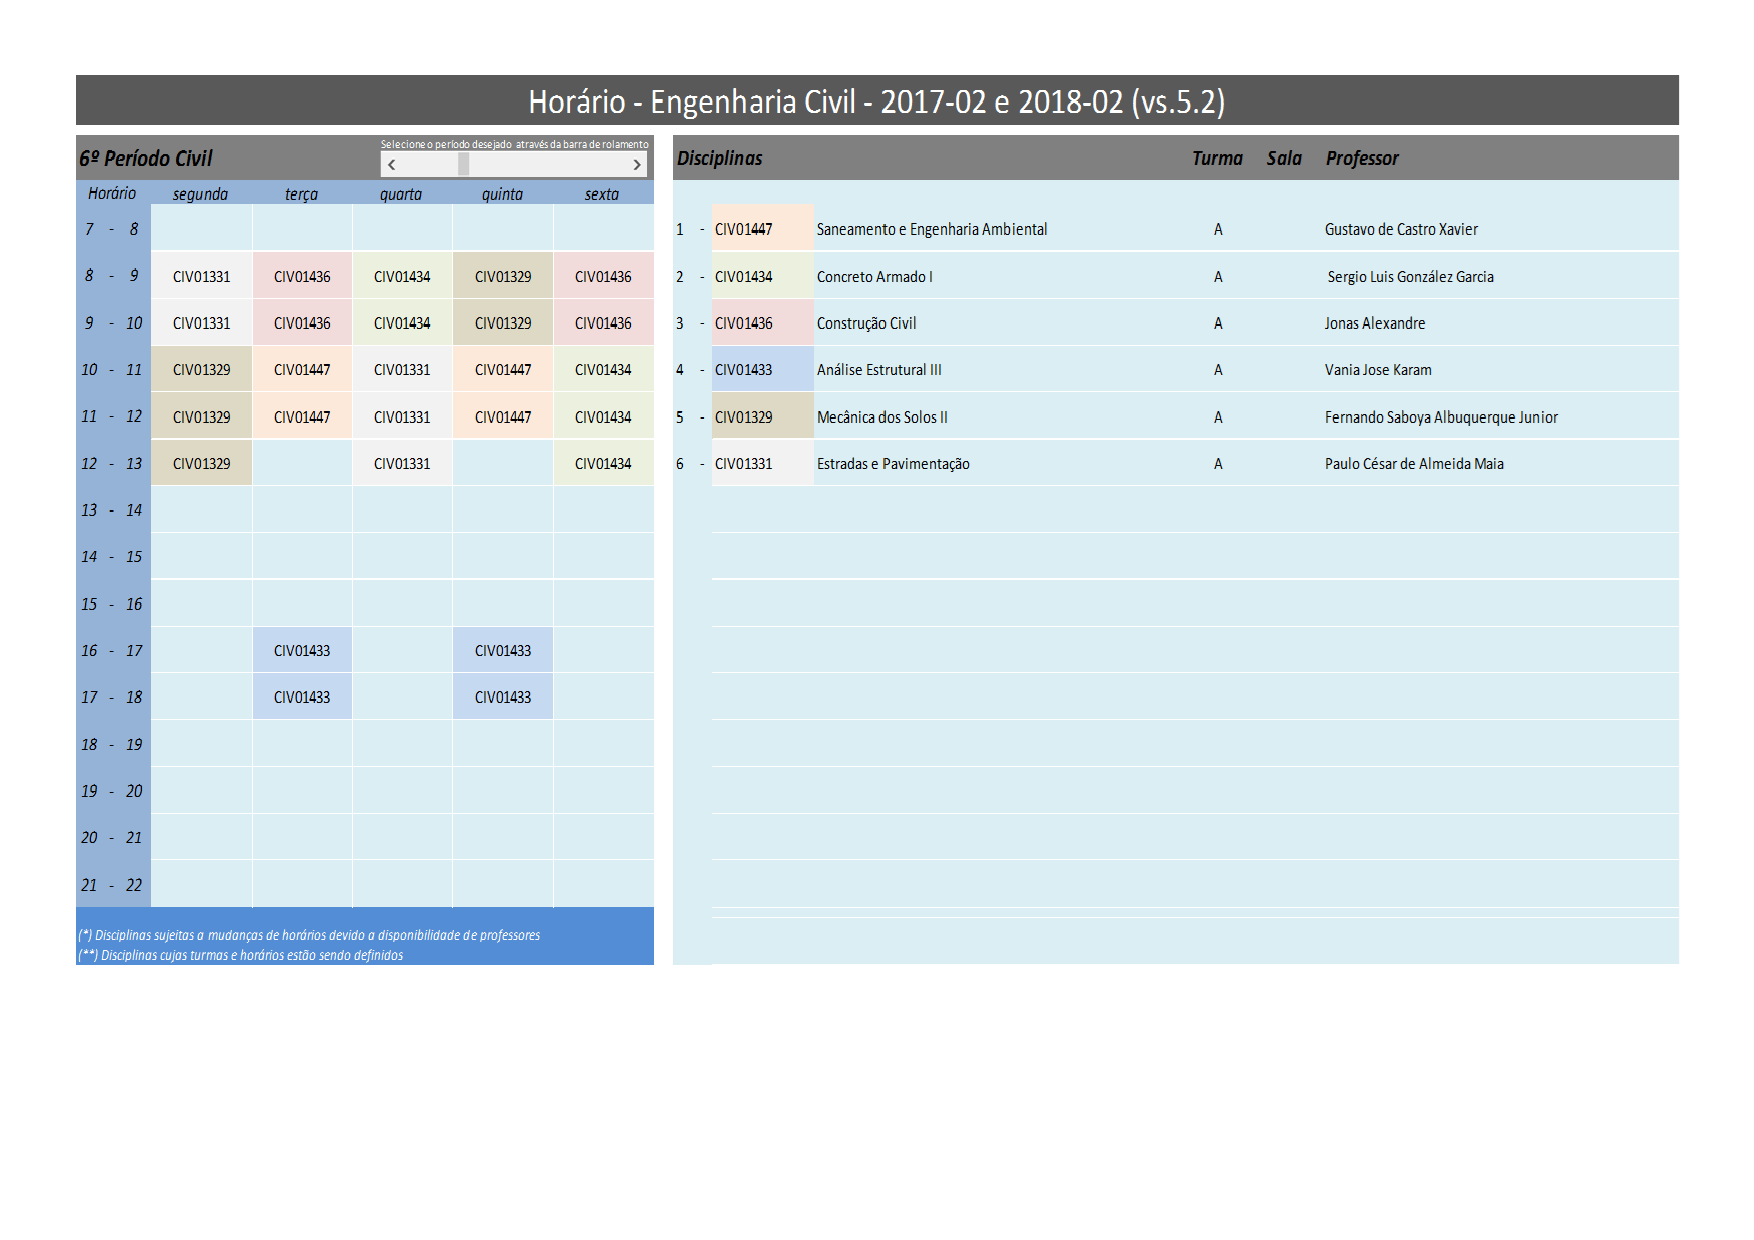
\includegraphics[width=\textwidth]{files/img/2.02!2-marco/GradeHoráriaLECIV}
  \legend{Fonte: \citeonline{Haddad2018}}
\end{CenteredFigure}

Quanto a análise desses documentos sobre esta grade algumas conclusões podem ser obtidas: 1. Esta forma de criação de grade foi mantida até no mínimo a data de 31/08/18 que consta no nome de um dos arquivos; 2. Foi utilizado o conceito de curva de nível com uma barra deslizante para visualizar a grade horária de cada período; 3. Com a legenda, entende-se que já se trabalhava com a ideia de maleabilidade de horários e também a ideia de alteração iterativa da grade; 4. Não se sabe ao certo se esta grade fora criada através de um software de criação de planilhas ou se foi criado através de um site.

Conclui-se então que esforços para se criar formas grades horárias intuitivas e maleáveis não estão limitados apenas ao curso de Ciência da Computação, também se estendendo a outros cursos da UENF.

\section{Estratégias de solução baseadas na otimização} \label{sec:teorias}                               % ###  2.5

Dentro do corrente trabalho, algumas teorias e métodos de resolução de problemas foram utilizados, sendo estes embasados por pesquisas anteriores.

\subsection{Relaxar restrições para encontrar soluções} \label{ssec:relaxar}                              % #### 2.5.1

Uma das formas de se encontrar soluções para problemas complexos é relaxando as restrições. Esse método consiste em ``permitir violações das restrições rígidas'' \cite{Dunke2023}, assim permitindo que soluções inviáveis sejam aceitas e posteriormente corrigidas.

Ao utilizar do método da programação inteira, \citeonline{Dunke2023} flexibilizam as restrições de seu modelo de programação linear, porém utilizam de uma heurística que corrige as soluções encontradas. De forma similar, \citeonline{Souza2000} menciona o uso de Algoritmos Genéticos que gera frequentemente soluções inviáveis, sendo utilizado então um filtro para que as inviabilidades sejam reparadas.

Com isso, entende-se que a flexibilização das restrições pode ser uma forma de se encontrar soluções viáveis. Ao permitir que esta categoria de soluções seja percorrida, abre-se a possibilidade de se encontrar outras soluções potencialmente viáveis que poderiam não ser encontradas de outra forma.

\subsection{Pontos de vista das dimensões do problema} \label{ssec:pontos}                                % #### 2.5.2

\citeonline{Piechowiak2004} lidam com a busca por uma solução para o problema de alocação de horários em universidades, utilizando-se de um sistema de suporte à decisão. Seu enfoque é em auxiliar o usuário em suas decisões, visando a interatividade, adaptabilidade e qualidades ergonômicas. Nele, o autor aborda a importância de se considerar que diferentes usuários têm diferentes pontos de vista e que devem cada um resolver sua parte local do problema em questão. O problema global é o \textit{design} e gestão das grades horárias de todos os recursos, entretanto, cada um dos ``gestores educacionais'' apenas veem uma parte do problema, porém, como os recursos são compartilhados, diversos conflitos acabam ocorrendo.

\subsection{Uso de soluções anteriores, soluções parciais e desvio de conflitos} \label{ssec:parciais}    % #### 2.5.3

\citeonline{Burke2000} consideram em seu trabalho o uso de casos preexistentes para que o problema encontre uma solução similar às anteriores. É visto com otimismo o uso da análise de grafos e sub-grafos como forma de se encontrar soluções parciais para o problema, pois permite a reutilização de soluções já processadas previamente. Em seu algoritmo, ao encontrar um sub-grafo similar ao problema atual, a solução é então adaptada para o problema atual. No caso da solução parcial encontrada apresentar conflitos, então as partes conflituosas são desalocadas, ordenadas da mais conflituosa pra menos conflituosa e então são realoacadas no primeiro horário viável.

\citeonline{Arratia2021, Miranda2012, Piechowiak2004, Burke2000} apontam a recorrência de instituições de ensino que utilizam as soluções anteriores como base para a criação de novas grades horárias. Pois, devido à similaridade do problema ao longo dos anos, é esperado que parte da busca por soluções seja facilitada pela reutilização de soluções anteriores.

\subsection{Informações ausentes e professores faltantes} \label{ssec:ausentes}                            % #### 2.5.4

\citeonline{Arratia2021} também citam em sua pesquisa a possibilidade de existirem turmas de determinadas disciplinas que não apresentam professores suficientes para ministrá-las. Neste caso, esta alocação é então marcada para que seja feita a distinção das demais. Assim gerando uma solução parcial para o problema, que pode ser resolvida posteriormente com a contratação de professores para ministrar as disciplinas faltantes.

\subsection{Sistemas de suporte à decisão} \label{ssec:sistemas}                                            % #### 2.5.5

O uso de sistemas de suporte à decisão é citado por \citeonline{Miranda2012} que menciona o uso de tais sistemas para o agendamento de cursos por mais de duas décadas. \citeonline{Piechowiak2004} também mencionam o termo, abordando em seu trabalho uma ferramenta de suporte a decisão que permite a alocação de horários evitando conflitos, mesmo que primeiro permita-se a existência deles, para que então sejam resolvidos. \citeonline{Frada2008} por sua vez definem o campo de Sistemas de Suporte à Decisão como ``uma disciplina aplicada que usa conhecimento e, especialmente, teoria de outras disciplinas''. Também é descrito como a forma ``como computadores e modelos analíticos podem ajudar os gerentes a tomar uma decisão-chave de planejamento de negócios recorrente'' \cite{Frada2008}.

\chapter{Modelagem geral do sistema} \label{chap:modelagem} % 3

% Tendo esclarecido sobre as \hyperref[chap:marco]{questões gerais da área de estudo} e de \hyperref[chap:instituicao]{como se estrutura a instituição} agora nos aprofundaremos na conceitualização do funcionamento geral do sistema e a forma como se dará a execução da \hyperref[sec:Metodologia]{metodologia proposta} apresentando o funcionamento geral de como o sistema será estruturado e de como foi desenvolvido.

Ao longo deste capítulo serão abordados os \hyperref[sec:estagios]{estágios de execução} sobre como se dão as etapas de criações de grade horária no geral, a \hyperref[sec:interacao]{interação} com os \textit{stakeholders}, o \hyperref[sec:funcionamento]{funcionamento} do sistema, o \hyperref[sec:ModelagemBD]{modelo de banco de dados} e a \hyperref[sec:REST]{API REST} que será utilizada para a comunicação entre o \textit{frontend} e o \textit{backend} do sistema.

\section{Estágios de execução} \label{sec:estagios} % 3.1

Em seu trabalho de aplicação prática, \citeonline{Miranda2012} estruturaram estágios que compõem o processo necessário para que enfim se alcance a definição de tabelas horárias finais.

\begin{CenteredFigure} \caption{Estágios para a obtenção de grade horária} \label{fig:geral}
  \includegraphics[width=\textwidth]{files/img/2.02!4-modelagem/Estágios Grade Final}
  \legend{Fonte: \citeonline{Miranda2012} - adaptado}
\end{CenteredFigure}

Na \autoref{fig:geral}, estão dispostos 4 estágios principais. O primeiro dispõe da aquisição de informações, sendo elas a disponibilidade do professor, os recursos da infraestrutura, as grades dos cursos, as estimativas de demanda e as políticas internas. No segundo estágio são definidas grades horárias preliminares com atribuição preliminar das salas. No terceiro, os alunos se inscrevem e a demanda é ajustada, por fim, no quarto estágio, ocorre a alocação final das salas. Com sua conclusão, são definidos as grades horárias finais junto com as respectivas salas.

A sequência geral condiz com o processo de criação das grades horárias, porém é necessário adaptar a metodologia para o contexto da UENF, e também ao escopo do trabalho. Os recursos de infraestrutura serão coletados dos histórico de alocação das turmas, a estimativa de demandas será obtida através da média histórica de alunos inscritos nas turmas e as políticas internas serão compreendidas através da revisão documental e entrevistas com os \textit{stakeholders}. O segundo tem caráter iterativo entre as coordenações e a diretoria do CCT. Os outros estágios não se distanciarão de forma significativa do que foi proposto.

\section{Interação} \label{sec:interacao} % 3.2

Para se alcançar uma alta satisfação por parte dos \textit{stakeholders}, vê-se necessária a constante interação com os mesmos. Para isto, será seguida a estrutura utilizada por \citeonline{Andre2018}.

\begin{CenteredFigure} \caption{Etapas do Design de Interação} \label{fig:IxD}
  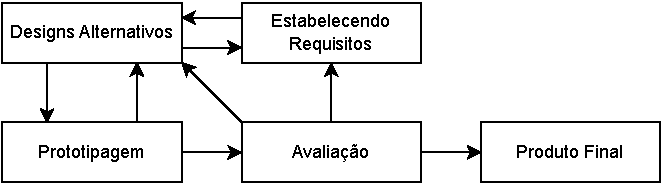
\includegraphics{files/img/2.02!4-modelagem/Arquitetura-IxD}
  \legend{Fonte: \citeonline{Andre2018} - adaptado}
\end{CenteredFigure}

Seguindo o conceito do Design de Interação, a \autoref{fig:IxD} ilustra o ciclo de ações a serem tomadas durante o desenvolvimento do sistema, caso este venha a ser necessário. Nesse modelo de pesquisa, os \textit{stakeholders} serão consultados continuamente enquanto lhes for apresentados protótipos do sistema, para que assim informem quanto às suas percepções. Esta dinâmica tem como finalidade encontrar um design tal que seja adequado aos desejos e necessidades de seus usuários. Pois, considerando que para que o sistema seja efetivo, é necessário que ele seja aceito e utilizado pelos usuários finais.

\section{Funcionamento} \label{sec:funcionamento} % 3.3

O sistema proposto funcionará de forma a auxiliar a coordenação do curso de Ciência da Computação da UENF na criação de grades horárias para os semestres letivos. Para isso, o sistema deverá ser capaz de gerenciar as informações referentes às disciplinas, professores, salas e horários disponíveis.

Para tanto, mesmo que disponha de informações pré-cadastradas, o sistema deverá permitir a inserção de novas informações, como disciplinas, professores e salas, pois, apesar de não ser o foco principal do sistema, é recorrente que haja alterações nessas informações ao longo do tempo, e caso o sistema não as comporte, não poderá cumprir seu propósito.

Como forma de agregar as informações cadastradas, o usuário será capaz de criar turmas para as disciplinas, informando o professor responsável, a sala e o horário em que a turma ocorrerá. Além disso, o sistema deverá permitir a visualização das turmas já cadastradas, bem como a edição e exclusão das mesmas, caso necessário. Ao criar uma turma, o sistema viabiliza a definição de qual ano e semestre a turma pertence.

As turmas contarão também com a informação de demanda estimada, que será utilizada como comparativo para a alocação das salas, de forma a evitar que uma sala seja alocada para uma turma cuja demanda seja maior do que a capacidade da sala. Outra informação contida nas turmas será um código descritor da turma em questão. Esse código será utilizado para auxiliar na compreensão das turmas, visto que ao longo do processo de criação das grades horárias é recorrente a criação de turmas criadas com um propósito específico, como por exemplo contemplar apenas repetentes ou alunos de um determinado conjunto de cursos.

Como ponto chave do funcionamento do sistema, o mesmo deverá ser capaz de ilustrar conflitos que vierem a surgir durante a alocação dos recursos. Esses conflitos podem ser de diversas naturezas, como por exemplo, a alocação de uma turma em um horário em que o professor responsável não está disponível, ou a alocação de duas turmas em uma mesma sala e horário. A identificação desses conflitos é essencial para que a coordenação possa corrigí-los de forma prática e direta, assim evitando que ocorram problemas durante a execução das turmas no semestre letivo.

Por fim, o sistema viabiliza também um método de rápida criação de turmas para todas as disciplinas esperadas para determinado semestre letivo para o curso de Ciência da Computação. Esse método consiste em analisar as disciplinas esperadas para os estudantes de computação em determinado semestre letivo, e, através do cálculo das maiores recorrências de professor, sala e horário atribuídos às turmas dessa mesma disciplina em semestres anteriores, criar uma turma com essas informações. Esse método visa agilizar o processo de criação das turmas, visto que a coordenação não precisará criar cada turma manualmente, mas sim apenas revisar as informações geradas pelo sistema.

Dispondo de todas essas funcionalidades, o sistema deverá ser capaz de gerar uma grade horária final, que será utilizada como base para a criação da grade horária oficial do curso de Ciência da Computação da UENF.

\section{Modelo de banco de dados} \label{sec:ModelagemBD} % 3.4

Considerando as informações necessárias para o presente trabalho, e também o preparo de campo para potenciais aplicações futuras, foi elaborado um diagrama conceitual parcial do banco de dados (\autoref{fig:DiagramConceitual}). Seu intuito foi trazer uma visualização mais clara das relações entre as entidades presentes no processo de criação de uma grade horária, e assim auxiliar na definição das tabelas que serão criadas no banco de dados \hyperref[ssssec:MySQL]{posteriormente}.

\begin{MyCenteredFigure} \caption{Diagrama Conceitual do banco de dados} \label{fig:DiagramConceitual}
  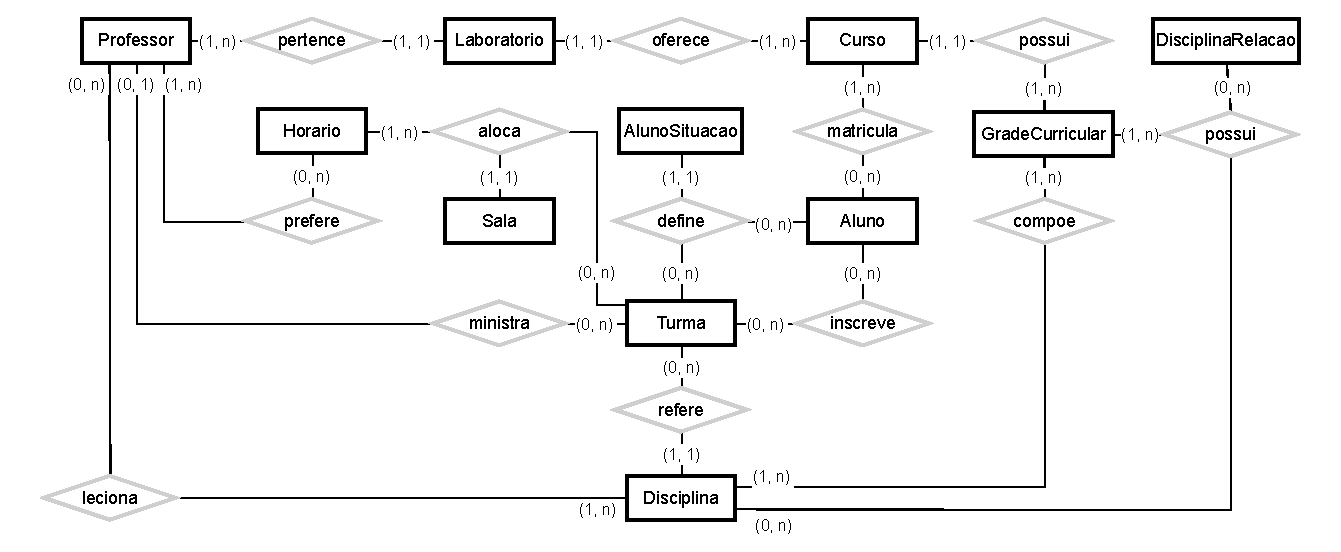
\includegraphics[width=\textwidth]{files/img/2.02!4-modelagem/Diagrama Conceitual}
\end{MyCenteredFigure}

O diagrama conceitual foi desenvolvido utilizando a ferramenta \LinkToURL{\LinkDrawio}{draw.io} e ilustra as relações entre diversas entidades presentes na realidade da UENF. O emaranhamento presente no diagrama ilustra a complexidade envolvida na criação de uma grade horária, onde diversas entidades se relacionam entre si.

Como principais apontamentos, podemos citar a parte principal do modelo que é a entidade \textbf{turma}. Ela, como já descrito, envolve a correlação entre alunos de diferentes cursos, professores, disciplinas, salas e horários. Além disso, também é possível notar a presença de entidades que não são diretamente relacionadas à alocação de turmas, mas que podem se mostrar úteis no futuro, como a relação entre professores e laboratórios; e a de disciplinas e ementas.

Embora o diagrama apresente uma visão mais completa das interconexões possíveis, é importante ressaltar que o presente trabalho foca primordialmente na alocação das turmas para o curso de Ciência da Computação, e que a implementação do banco de dados será feita de forma a atender a essas necessidades, fazendo então uso de apenas uma parte do diagrama conceitual apresentado pela \autoref{fig:DiagramConceitual}.
Sendo posteriormente ilustrados na \autoref{ssec:MVP2} pela \autoref{fig:TabelasIniciais}, na \autoref{ssec:MVP3} pela \autoref{fig:MVP3_BancoDeDados} e na \autoref{ssec:Funcionalidades preparadas} pela \autoref{fig:DER final}.
% Sendo posteriormente ilustrados na \hyperref[ssec:MVP2]{subseção ``Versão 2.0''} pela \autoref{fig:TabelasIniciais}, na \hyperref[ssec:MVP3]{subseção ``Versão 3.0''} pela \autoref{fig:MVP3_BancoDeDados} e na \hyperref[ssec:Funcionalidades preparadas]{subseção ``Funcionalidades preparadas''} pela \autoref{fig:DER final}.

% DEIXAR MAIS DESCRITO EM QUE SEÇÃO ESSAS FIGURAS ESTÃO.

% \subsection{Diagrama de Entidade e Relacionamento} % 3.4.1

% Neste modelo, mais enxuto, temos apenas as entidades principais, onde temos uma turma de determinada disciplina, ministrada por um professor e que ocorre em uma sala em um determinado horário.

% Neste diagrama vemos as entidades principais, que são \textbf{Turmas}, \textbf{Disciplinas}, \textbf{Professores}, \textbf{Horários} e \textbf{Salas}. As propriedades escolhidas para cada entidade são compostas por uma mistura de critérios. Por exemplo, o nome do professor, o código da disciplina, e a junção de código e bloco auxiliam primordialmente na identificação real dos professores, disciplinas e salas. Já as informações ``período'', ``apelido'' e ``comment''...

% E também é notável a presença da entidade \textbf{Alunos}, que se apresenta desacoplado das demais entidades. O motivo para isso é que, embora os alunos façam parte do processo de alocação de turmas, ao longo do desenvolvimento, o desenvolvimento de funcionalidades envolvendo os alunos...

\section{API REST} \label{sec:REST} % 3.5

Para exemplificar o funcionamento geral da permanência dos dados, consideremos o uso de uma \textit{API REST} utilizando de 4 ``camadas'': o \textbf{\textit{frontend}}, os \textbf{\textit{endpoints}}, as \textbf{funções} de execução e o \textbf{banco de dados}.

% Essa parte sobre Dev e Prod tá muito deslocada
% Ele se encontra em duas formas: a primeira é o chamado ``em produção'', que é o sistema que o usuário final acessa, e a segunda é o chamado ``em desenvolvimento'', que é o sistema que o desenvolvedor acessa para realizar as modificações necessárias. Ambas precisam

O \textbf{\textit{frontend}} é a interface do sistema, onde o usuário interage com o sistema. Essa interface precisa se comunicar com o \textit{backend} para realizar as quatro operações básicas no banco de dados (criação, leitura, atualização e deleção) por sobre as entidades existentes (turmas, professores, disciplinas, salas, etc.). Elas assim o fazem ao enviar requisições HTTP (\textit{GET}, \textit{POST}, \textit{PUT} e \textit{DELETE}), contendo pacotes de informações em formato JSON para os \textbf{\textit{endpoints}}.

Os \textbf{\textit{endpoints}} são as rotas que o \textit{backend} disponibiliza para a recepção das requisições HTTP. Eles são responsáveis por encaminhar as requisições recebidas. Seu funcionamento consiste em rotear as requisições recebidas junto com sua carga útil. Para tanto, as rotas criadas refletem diretamente a qual entidade do banco de dados a requisição se refere, sendo então assim sabido qual \textbf{função} deve ser executada.

As \textbf{funções} são as responsáveis por executar as operações no banco de dados. Elas processam o pacote de informações recebido, e então realizam a operação desejada no \textbf{banco de dados}.

O \textbf{banco de dados} recebe a requisição, processa a operação, e então retorna o status da operação. Esse retorno é então repassado camada por camada, até chegar ao \textit{frontend}, onde o usuário final pode visualizar o resultado da operação.

\textbf{Resumidamente}: O \textbf{\textit{frontend}} envia uma requisição HTTP com uma carga de informações a um \textbf{\textit{endpoint}}, que encaminha a requisição a uma \textbf{função} específica que executa uma operação no \textbf{banco de dados}, assim retornando o status da operação ao \textit{frontend}.

\section{Diferença dos trabalhos anteriores} \label{sec:diferenca} % 3.6

Os trabalhos mais próximos ao presente, quanto a instituição são os trabalhos feitos por \citeonline{SanyaSantos2013} e \citeonline{RicardoSilveira2014}, porém, o presente trabalho se distingue em algumas questões.

Talvez uma das mais marcantes distinções é a visualização presente nos dois trabalhos anteriores onde são considerados um limite de cinco disciplinas por horário, pois ambos consideram em seus trabalhos que o curso de computação está dividido entre as cinco turmas de cada grupo de períodos, sejam as do semestre ímpar (1, 3, 5, 7 e 9) ou as do semestre par (2, 4, 6, 8 e 10). No entanto, o presente trabalho avalia que, é mais condizente com a realidade da instituição se for considerado que os alunos tendem a não seguir completamente essa subdivisão, tendendo a ficar com disciplinas de semestres diferentes geralmente aquém do esperado, mas também podendo estar além do que se espera.

Outra característica marcante é a dependência de salas disponíveis que comportem o número de alunos esperados para a turma, o que não é considerado pelos autores, visto que esta característica não é vista como pertencente ao escopo da Coordenação do Curso de Ciência da Computação. Já neste trabalho, considera-se que esta informação é essencial para que haja a confirmação da validade da alocação da turma. Além disso, como existem diversos outros cursos que utilizam as salas do CCT, é importante que a coordenação tenha conhecimento sobre a disponibilidade das salas para que possa alocar as turmas de forma eficiente, sendo então necessário o preenchimento de informações sobre as disciplinas necessárias para os outros cursos.

Existem também alguns critérios usados por \citeonline{SanyaSantos2013} e \citeonline{RicardoSilveira2014} que não são considerados no presente trabalho, como a preferência de professores associados e professores contratados, e o desejo por se evitar alocar disciplinas que possuam aulas em horários próximos ou que sobreponham o horário de almoço.

\chapter{Coleta de informações sobre a instituição} \label{chap:instituicao} % ## 4

% Como citado pelos autores [FAZER REFERÊNCIA À TODOS OS AUTORES QUE FALAM DISSO], o
O problema de criação de grade horária tem forte influência da estrutura organizacional da instituição. Por tal motivo, este capítulo tem como objetivo apresentar a estrutura organizacional da \LinkToURL{\LinkSiteUENF}{Universidade Estadual do Norte Fluminense Darcy Ribeiro (UENF)} e como se dá o processo de criação de grades horárias na mesma. Essa apresentação se mostra necessária para que se possa entender melhor o problema e as possíveis soluções.

A apresentação se dará em três partes principais: a explanação sobre \hyperref[sec:estatuto]{como a UENF está definida segundo seus documentos oficiais}, a análise qualitativa das \hyperref[sec:entrevistas]{entrevistas realizadas com os principais envolvidos no processo de criação de grades horárias} e a análise quantitativa das respostas do \hyperref[sec:formulario]{questionário aplicado aos alunos da UENF}. Os dois primeiros tópicos convergem na criação de uma \hyperref[sec:sequencia]{sequência de criação de grades horárias}. Por fim, será apresentada a análise das \hyperref[sec:relacoes]{relações entre as variáveis} envolvidas no processo de criação de grades horárias.

% Vindo da introdução:
% Essas informações serão relevantes para se atingir a satisfação e uso futuro do sistema proposto.
% Espera-se com este capítulo fornecer um entendimento amplo e, ao mesmo tempo, focalizado o bastante, para que se possa compreender claramente o processo de criação de grades horárias na UENF e os fatores que o influenciam.

\section{A UENF} \label{sec:estatuto} % ### 4.1

A UENF conta com diversos documentos que visam regulamentar e explicar seu funcionamento. Os documentos vão desde o mais alto nível onde se atribui as funções da UENF, até o menor nível onde se mostra a Grade Curricular para o curso de Ciência da Computação. Desses documentos, podemos listar o Estatuto da UENF \cite{Estatuto2002}, o Plano de Desenvolvimento Institucional \cite{PDI2023}, o Regimento Geral da UENF \cite{RegimentoGeralUENF2006}, o Regimento Geral da Graduação \cite{RegimentoGeralGraduação2012}, o Regimento da Câmara de Graduação \cite{RegimentoCâmaraGraduação2012}, as Normas da Graduação \cite{Normas2012}, os Projetos Pedagógicos do Curso de Ciência da Computação \cite{PPCCC2005, PPCCC2015, PPCCC2022} e a Matriz Curricular do Curso de Ciência da Computação \cite{Matriz2015}.

% Provavelmente eu deveria adicionar informações sobre a secretaria acadêmica
% Precisa de revisão
% Sinto que falta falar sobre secretaria acadêmica e Conselho de Centro

Segundo o estatuto, a UENF compreende os \textbf{Órgãos da Administração Superior de política, gestão e supervisão}; \textbf{Unidades universitárias de ensino, pesquisa e extensão}; e os \textbf{Órgãos e serviços especiais, destinados a auxiliar na administração e a suplementar as atividades de ensino, pesquisa, extensão e apoio técnico}.

Quanto aos órgãos da Administração Superior devemos enfocar o órgão executivo, constituído unicamente pela reitoria, cujos órgãos auxiliares englobam a Secretaria Acadêmica, que por sua vez tem como algumas de suas atribuições as seguintes: Coordenar a \textbf{divulgação do horário escolar dos vários cursos da UENF}, de modo a \textbf{otimizar os recursos humanos}, \textbf{ampliar as opções de disciplinas para os alunos} e tornar acessíveis os dados escolares; e \textbf{Centralizar os serviços de registro da vida escolar dos alunos}, compreendendo \textbf{inscrição}, admissão, \textbf{matrícula}, \textbf{créditos}, \textbf{opções}, transferências, promoções, graduações e preparação dos respectivos diplomas, dentro das normas estabelecidas.

Já quanto as unidades universitárias de ensino, temos no estatuto que ``as unidades universitárias de ensino, pesquisa e extensão, definidas por áreas de conhecimento, são constituídas em Centros, que por sua vez congregam Laboratórios afins'' e que ``o Laboratório é a menor parte da estrutura universitária para todos os efeitos de organização administrativa, didático-científica, distribuição de pessoal e de representação nos órgãos colegiados da UENF''.

A administração do Centro é da competência do Diretor e seu Conselho. Os Laboratórios, por sua vez, são administrados pelos Chefes de Laboratório.

O Conselho de Centro, tem como uma de suas atribuições, descrito no inciso XVII do artigo 34 do estatuto, a seguinte: \textbf{designar, semestralmente, os professores responsáveis pelas disciplinas dos Cursos de Graduação} e Programas de Pós-Graduação, ouvidos os respectivos Laboratórios, os Colegiados de Curso e Comissões de Coordenação. Atualmente, segundo o site da UENF, a universidade possui 4 Centros, sendo eles: Centro de Ciências do Homem - \LinkToURL{\LinkCCH}{CCH}; Centro de Ciência e Tecnologia - \LinkToURL{\LinkCCT}{CCT}; Centro de Biociências e Biotecnologia - \LinkToURL{\LinkCBB}{CBB}; Centro de Ciências e Tecnologias Agropecuárias - \LinkToURL{\LinkCCTA}{CCTA}.

E também existem 8 \LinkToURL{\LinkLaboratorios}{laboratórios} vinculados ao Centro de Ciência e Tecnologia (CCT), sendo eles:

\begin{enumerate}[nosep]
  \item Laboratório de Meteorologia – \LinkToURL{\LinkLAMET}{LAMET};
  \item Laboratório de Ciências Físicas – \LinkToURL{\LinkLCFIS}{LCFIS};
  \item Laboratório de Engenharia Civil – \LinkToURL{\LinkLECIV}{LECIV};
  \item Laboratório de Ciências Químicas – \LinkToURL{\LinkLCQUI}{LCQUI};
  \item Laboratório de Materiais Avançados – \LinkToURL{\LinkLAMAV}{LAMAV};
  \item Laboratório de Ciências Matemáticas – \LinkToURL{\LinkLCMAT}{LCMAT};
  \item Laboratório de Engenharia de Produção – \LinkToURL{\LinkLEPROD}{LEPROD};
  \item Laboratório de Engenharia e Exploração de Petróleo – \LinkToURL{\LinkLENEP}{LENEP}.
\end{enumerate}

Os Laboratórios englobam os Cursos de Graduação e Pós-Graduação, que são administrados pelos Coordenadores de Curso. Além disso, o LCMAT mantém dois cursos de graduação e um programa de pós-graduação stricto sensu. Sendo eles:

\begin{enumerate}[nosep]
  \item \LinkToURL{\LinkLicMat}{Licenciatura em Matemática};
  \item \LinkToURL{\LinkSiteCCUENF}{Bacharelado em Ciência da Computação};
  \item \LinkToURL{\LinkLCMATPósGraduação}{Mestrado Profissional em Matemática} – \LinkToURL{\LinkUENFPósGraduações}{PROFMAT} / \LinkToURL{\LinkProfMat}{SBM}.
\end{enumerate}

\subsection{Responsáveis pela criação das grades horárias} \label{ssec:responsaveis} % #### 4.1.1

As atribuições de cada setor estão, em sua maioria, descritas nas documentações encontradas. De forma resumida suas as atribuições são:

\begin{itemize}
  \item \textbf{Secretaria Acadêmica}: elaborar e divulgar o Calendário Acadêmico; otimizar os recursos humanos; ampliar a oferta de disciplinas;
  \item \textbf{Câmara de Graduação}: aprovar e modificar o calendário acadêmico; sugerir vagas de bolsistas;
  \item \textbf{Direção de Centro}: designação semestral de professores responsáveis pelas disciplinas, após ouvir os Laboratórios, Colegiados e Coordenações;
  \item \textbf{Chefia do Laboratório}: atribuir carga horária didática aos docentes do laboratório e aos bolsistas; designar docente responsável por disciplina ofertada;
  \item \textbf{Coordenação do Curso}: coordenar a distribuição de estudantes do curso; indicar à chefia de laboratório as disciplinas a serem ofertadas ao curso coordenado;
  \item \textbf{Sistema Acadêmico}: articula parcialmente as informações entre os setores, como a oferta de disciplinas e a distribuição de estudantes.
\end{itemize}

\section{Entrevistas} \label{sec:entrevistas} % ### 4.2

% Separar entrevistas de minhas opiniões pessoais

Como forma de entender melhor a percepção real daqueles que recorrentemente lidam com a tarefa de criação da grade horária, diversas entrevistas foram feitas com o intuito de analisar qualitativamente quais são as opiniões, pedidos, reclamações e pensamentos de diferentes níveis organizacionais da UENF. Essas análises têm como objetivo principal averiguar se o processo de criação de grades horárias realizada na UENF se apresenta como uma tarefa problemática e se a solução proposta neste trabalho se mostra como uma solução viável.

Pois, como é informado por \citeonline{PierreSWEBOK2014}, uma das fontes de requisitos é o ambiente organizacional e como o \textit{software} muitas vezes visa auxiliar em algum processo da instituição, processo este já condicionado à sua estrutura, cultura e políticas externas, o engenheiro de \textit{software} precisa estar atento a elas, visto que o novo \textit{software} não deve forçar mudanças não planejadas em processos de negócios.

\subsection{Direção do CCT} \label{ssec:3_Diretor} % #### 4.2.1

O primeiro entrevistado, em 7 de agosto de 2023, foi o Diretor do CCT. Ele atualmente estrutura a relação de disciplinas ofertadas pelo CCT em Excel e as publica \LinkToURL{\LinkDistribuiçãoDeSalas}{em formato PDF no site do CCT}. Seu trabalho auxilia os Chefes de Laboratório e Coordenadores de Curso a visualizarem quais são as salas disponíveis e em quais horários cada professor está alocado.

Um dos tópicos dialogados, foi quanto às categorias das disciplinas, ou seja, quais características notáveis as disciplinas poderiam ter. Com isso podemos listar as seguintes categorias de disciplinas:

\begin{itemize}[nosep]
  \item \textbf{Anuais}: disciplinas que ocorrem apenas uma vez no ano;
  \item \textbf{Ímpares}: disciplinas que são ofertadas no primeiro semestre letivo;
  \item \textbf{Pares}: disciplinas que são ofertadas no segundo semestre letivo;
  \item \textbf{De serviço}: disciplinas ofertadas para mais de um curso simultaneamente;
  \item \textbf{Ciclo básico}: disciplinas oferecidas para todas as engenharias;
  \item \textbf{Repetentes}: turmas criadas especialmente para repetentes.
\end{itemize}

As disciplinas ímpares e pares geralmente estão atreladas à expectativa de que os alunos progredirão sequencialmente sem reprovação alguma. Entretanto, caso uma quantidade de alunos considerável de alunos reprove em determinada disciplina, é possível que estes se enquadrem na criação de uma turma especial para repetentes, ou não.

Uma sugestão de utilidade para o software é a de permitir que as ``disciplinas de serviço'' sejam fixas, visto que estas são as que têm maior complexidade de manejamento de horário posteriormente, justamente por geralmente abrangerem muitos alunos e de diversos cursos diferentes.

Uma outra característica notável é a repetição de atribuições de disciplinas em pares regulares, ou seja, alocadas no mesmo período de horário com um dia de intervalo entre elas. Um exemplo desse tipo de alocação recorrente seria ``14 às 16 horas de segunda e quarta feira''.

Com isso, surge a dúvida: há uma preferência ativa por aulas alocadas com este padrão? A resposta dada é que não. O que se mostra como uma restrição a menos na hora de se alocar as turmas.

Outro caso notável é a existência majoritárias de turmas criadas com dois períodos de duas horas, entretanto existem algumas que fogem deste padrão e possuem três horas de duração. A solução encontrada pelo Diretor é a de colocar esta disciplina começando às 10h, o que faz com que se alongue até as 13h, período geralmente usado pelos estudantes e servidores para se alimentar, e justamente por isso evitando que atrapalhe a distribuição das salas. Outra alternativa é alocar esta turma para as 13h, fazendo com que finalize às 16h, horário em que as disciplinas com duas horas de duração geralmente terminam.

Segundo ele, saber a demanda máxima possível seria bom, visto que podem haver casos de solicitações de vagas para disciplinas de serviço que extrapolam a quantidade esperada para a distribuição balanceada dentre os cursos.

Uma outra situação que ocorre é que algumas disciplinas historicamente têm seus horários definidos em um mesmo horário ao longo dos anos. Caso essa alocação seja alterada, ocorre a possibilidade de reclamação por parte dos professores, mesmo que esta alteração seja benéfica para os estudantes. Então por exemplo, os horários de 8h de uma segunda feira e de 16h de sexta feira, não são geralmente desejados pelos professores, mesmo que eles teoricamente tenham disponibilidade de 8 horas diárias.

Considerando a quantidade de laboratórios ``concorrendo'' simultaneamente às vagas, surge a dúvida: há ordem de precedência entre os laboratórios? A resposta para esta pergunta é ``Não. As vagas são distribuídas com prioridade na ordem de chegada''.

Algumas outras informações que ele elenca:

\begin{itemize}
  \item \textbf{As turmas de disciplinas básicas são grandes}: é esperado que uma grande quantidade de alunos se inscreva nas turmas de disciplinas essenciais e iniciais de seus cursos, sendo boa parte dela relacionada com o conceito das disciplinas de serviço e com o conceito de ciclo básico das engenharias;
  \item \textbf{As turmas de disciplinas de serviço devem ser alocadas primeiro}: visto a grande quantidade de conflitos possíveis dentre os diversos cursos, ao alocá-las primeiro, os conflitos passam a ocorrer em turmas com uma quantidade menor de pessoas e/ou que sejam de um mesmo curso;
  \item \textbf{As alterações vão até o final do período}: embora possa parecer que a alocação de turmas finalize após o encerramento do período de inscrição e desinscrição, na prática, a realocação ocorre durante todo o período;
  \item \textbf{Teoricamente matérias de um mesmo período não devem conflitar}: isso se dá segundo a percepção de que a maioria dos alunos está seguindo a mesma linha sequencial de disciplinas, o que muitas das vezes não é a realidade.
\end{itemize}

\subsection{Desenvolvedor do Sistema Acadêmico} \label{ssec:3_Desenvolvedor} % #### 4.2.2

Considerando que a integração do sistema proposto seria certamente mais eficiente se integrada ao sistema acadêmico, viu-se como apropriado entrevistar o desenvolvedor do Sistema Acadêmico para se ponderar sobre o uso dos dados e a possível integração.

Durante a entrevista, realizada no dia 21 de agosto de 2023, foram listados alguns dados que seriam interessantes para a análise, sendo eles a demanda de disciplinas, a listagem dos professores, a listagem dos alunos aprovados e suas respectivas disciplinas e por fim os requisitos das disciplinas.

% - Demanda de disciplinas
% - Listagem de professores
% - Listagem dos alunos aprovados
% - Requisitos das disciplinas

Outra questão analisada seria quanto a forma de integração. Boa parte das aplicações web se comunicam em forma de API, entretanto, devido à quantidade de alterações executadas ao longo do semestre no sistema acadêmico, o Desenvolvedor do Sistema Acadêmico utiliza o sistema de mensagerias através do \LinkToURL{\LinkRabbitMQ}{RabbitMQ}.

Foi citado sobre a abordagem do Coordenador de Computação para o cálculo das demandas, quanto a isso, o Desenvolvedor citou que poderia facilmente permitir o download de um CSV dos dados necessários.

Quanto à possibilidade de aprimoramentos no Sistema Acadêmico, ele disse que ``eu faço o que me pedem'', se referindo ao repositório do Acadêmico disponível no \LinkToURL{\LinkGitLab}{GitLab}, onde alguns poucos usuários fazem solicitações de alterações e melhorias. Havendo então a possibilidade de que o Coordenador de Computação faça uma solicitação à SECACAD para que seja implementada uma funcionalidade que permita a exportação dos dados necessários para o cálculo das demandas.

Um outro problema apontado por ele é a falta de gente. Segundo ele, outras duas pessoas entraram junto com ele no mesmo concurso, mas foram realocadas para outras áreas da universidade. Ele cita também sobre a ``cultura do trabalho opcional'' existente na UENF, onde muitos servidores não se sentem obrigados a trabalhar.

Em relação a estrutura dos dados, o sistema acadêmico utiliza o SQL. Foi citado o uso de NOSQL e estrutura de Grafos como possibilidades de mudança, mas como a mesma não se mostrou necessária até o momento, não foi implementada.

Uma questão levantada pelo entrevistado diz respeito à manutenção do software desenvolvido neste trabalho. Não sabendo ele dizer se o mesmo seria mantido pela UENF.

Ele também sugere que, para evitar a complexidade de se trabalhar com dados reais de alunos, que sejam utilizados dados fictícios.

\subsection{Chefia de Laboratório de Matemática} \label{ssec:3_Chefe} % #### 4.2.3

Considerando que um dos cargos relacionados com o processo de elaboração de grades horários é o de Chefe de Laboratório, em 25 de agosto de 2023, foi entrevistada a atual Chefe de Laboratório de Matemática.

Assim como sugerido pelo Desenvolvedor do Sistema Acadêmico, a Chefe também sugeriu que dados fictícios fossem utilizados. Sugeriu ainda que fosse utilizado o schema do banco de dados do sistema acadêmico como sua criação. Outra sugestão foi a solicitação ao Desenvolvedor do Sistema Acadêmico uma listagem de possíveis valores recorrentes no banco de dados.

A entrevistada também relatou algumas problemáticas envolvendo a realocação dos horários das turmas. Segundo ela, qualquer alteração pode ser feita durante a semana anterior à matrícula, visto que, não havendo inscritos, não há problema na alteração. A partir do momento em que houver ao menos um aluno inscrito na disciplina, alterações só podem ser feitas caso não haja conflitos aparentes e preferencialmente com um documento assinado pelos alunos que estiverem inscritos.

\subsection{Responsável pela Secretaria Acadêmica (SECACAD)} \label{ssec:3_Responsável} % #### 4.2.4

No dia 1 de setembro, o responsável pela Secretaria Acadêmcia foi entrevistado. Inicialmente, alguns tópicos foram trazidos como ponto focal da entrevista, sendo alguns deles os seguintes:

\begin{itemize}
  \item Dúvidas quanto as atribuições da SECACAD;
  \item Permissão de acesso aos dados que não são estritamente necessários, mas ajudariam;
  \item Definição dos períodos, demanda provisória e erros de estimativa;
  \item GitLab, tarefas (issues) e demandas;
  \item Automatização da burocracia;
  \item Ética VS Eficiência.
\end{itemize}

Logo de início, o entrevistado informou que ele não pode ceder dados de nenhum aluno, mesmo que anonimizados, mas sugeriu que poderia reencaminhar um formulário de pesquisa para os alunos, para que assim eles próprios pudessem fornecer os dados necessários.

Outra abordagem interessante informada por ele é quanto ao seu conhecimento técnico, onde sugeriu abordagens de análise multicritérios como forma de se auxiliar a criação das grades horárias.

Durante a conversa, foi citado de forma positiva quanto à demanda exata de cada disciplina. Reforçou-se a preferência pela alocação de disciplinas visando os estudantes mais próximos da conclusão do curso, estando em último na ordem de prioridade aqueles que decidem se adiantar com disciplinas de períodos mais avançados. Uma outra característica apontada é que a sequência de definições é a seguinte: Vagas $\rightarrow$ Professor $\rightarrow$ Sala $\rightarrow$ Horário.

Também se confirmou a não existência de um registro oficial das salas e suas capacidades. Essa informação é inserida como um campo de texto no sistema acadêmico, com isso, o sistema não impediria a alocação de duas turmas em uma mesma sala em um mesmo horário.

O responsável pela SECACAD também informou que cabe à Pró-Reitoria a mudança do início do primeiro semestre para expandir o período de preparação das grades horárias para o segundo período, sendo que este pedido deve partir da Câmara de Graduação.

Quanto ao tópico ``ética VS eficiência'', ele citou que embora o sistema acadêmico impeça a realocação de turmas com alunos inscritos, é possível que o mesmo seja burlado ao manualmente se excluir a inscrição do aluno. Sendo esta prática justificável em alguns casos.

Uma ferramenta que o beneficiaria seria a análise dos alunos que estão à beira de perder o vínculo com a universidade, para que a Secretaria Acadêmica possa tomar as medidas cabíveis.

\subsection{Coordenação de Computação} \label{ssec:3_Coordenador} % #### 4.2.5

Sendo o Coordenador de Computação o principal usuário do sistema, torna-se imprescindível a análise qualitativa de sua perspectiva.

Seguindo o conceito de Design Interativo utilizado também por \citeonline{Andre2018}, o Coordenador foi consultado em diversas etapas do desenvolvimento do sistema. Diversos encontros foram realizados, sendo iniciado em 1 de agosto de 2023. Inicialmente, foi apresentado a ele o conceito do sistema, suas funcionalidades e possíveis benefícios. Em seguida, foi apresentado a ele um protótipo do sistema. Mas esta questão será melhor tratada em outro segmento deste mesmo trabalho, aqui será abordado apenas o conteúdo das entrevistas.

Assim como comentado pelo Diretor do CCT, o Coordenador também fala sobre a definição de matérias que se mostram fixas, porém, agora com outro olhar: enquanto o diretor vê as matérias fixas como uma forma de atribuição histórica, o Coordenador por sua vez vê apenas como uma forma predefinida e imutável. Porém, olhando em um contexto mais amplo, essa definição de matérias não se mostra como obrigatória, visto que pode haver casos em que outra alocação de uma disciplina ``fixa'' apresente uma qualidade melhor do que seu horário usual. Segundo ele, ``Houve uma resolução anos atrás para que os horários ficassem fixos''.

Outra questão levantada por ele é quanto a um problema já antigo no curso de Ciência da Computação na UENF, que há anos apresenta um corpo docente reduzido em comparação com outros cursos, sendo necessário um desdobramento maior para suprir a demanda de disciplinas dos alunos. Uma solução utilizada é a de solicitar a abertura de uma bolsa de apoio ao ensino, onde qualquer professor de pós-graduação, preferencialmente com mestrado, pode ser alocado como professor de uma disciplina. Solução que embora não seja a ideal, é a que se mostra mais viável.

Uma outra característica até então não citada pelos outros entrevistados é que existem salas que são vistas culturalmente como sendo de determinado curso, onde acaba sendo um certo tabu a alocação de uma disciplina de outro curso, mesmo que não se esteja infringindo regra alguma.

Quanto à priorização de veteranos já citada anteriormente, o Coordenador aponta uma outra forma de se enxergar a situação: em disciplinas dos períodos finais do curso, a prioridade é dos veteranos, ficando os calouros que ocasionalmente possam ter se adiantado, em segundo plano. Já em disciplinas dos períodos iniciais, a prioridade é dos calouros, ficando os veteranos que por ventura tenham reprovado, em segundo plano.

Diferente de como foi respondido pelo Diretor do CCT, para o Coordenador de Computação a alocação de disciplinas em pares se mostra como ``didática'', sendo ela então preferível, mas não necessariamente vista como obrigatória.

Considerando a recorrência de citação do conceito de estimativas de demanda, o Coordenador de Computação sugere que haja um campo no sistema para que seja inserida a demanda estimada de cada disciplina.

Considerando que no contexto atual do curso de Ciência da Computação na UENF é iminente a adoção de uma nova grade curricular, o Coordenador apresentou preocupação em relação à possibilidade de que o sistema não seja mais utilizado após a adoção da nova grade. Essa questão encontra-se atualmente fora do escopo do atual projeto, entretanto, não se mostra como um problema de difícil solução, visto que o sistema pode ser adaptado para a nova grade.

\subsection{Entendimento geral das entrevistas} \label{ssec:conclusaoEntrevistas} % #### 4.2.6

Podemos concluir após a análise qualitativa das entrevistas que há de fato um certo grau de insatisfação por parte dos usuários do sistema atual. Embora o sistema funcione, ele apresenta gargalos que poderiam ser resolvidos com a utilização de um sistema mais eficiente que envolvesse as diferentes partes interessadas. Suas maiores insatisfações são quanto à burocracia e o curto período de tempo disposto para a elaboração das grades horárias.

Embora não sejam apontadas como insatisfação, algumas potenciais ferramentas e melhorias foram também citadas pelos entrevistados. Dentre elas, a demanda máxima possível, que passaria a evitar superestimações de demanda, a alocação de disciplinas de serviço como fixas, e em alguns casos, a alocação de disciplinas em pares de horários, que embora não seja uma regra, é uma preferência de um dos entrevistados. Outra ferramenta que foi citada é a de análise de alunos à beira de perder o vínculo com a universidade, que poderia ser utilizada pela Secretaria Acadêmica para tomar as medidas cabíveis. Também se fazendo notória a necessidade de registro oficial das salas e suas capacidades, que atualmente é inserida como um campo de texto no sistema acadêmico.

Outros problemas encontrados, remetem à acomodação institucional de algumas práticas, como a alocação de disciplinas em horários fixos, em pares e/ou nas mesmas salas. Essas práticas, embora não sejam obrigatórias, são vistas como um costume e por isso são mantidas.

\section{Sequência de criação das grades horárias} \label{sec:sequencia} % ### 4.4

% Estou com dúvida novamente de qual é a progressão e de quem faz o quê

Ao somarmos o conhecimento presente no estatuto da UENF, com o conhecimento adquirido através das entrevistas, podemos ter uma visão geral de como se dá a criação das grades horárias na UENF. Assim, abaixo estão listadas as etapas pelas quais geralmente se passam para a criação das grades horárias.

\begin{enumerate}
  \item Período ocorrendo normalmente;
  \item Coordenadores enviam para Chefes de Laboratório uma demanda estimada de cada uma das disciplinas que serão ofertadas;
  \item Chefes de Laboratório atrelam professores a disciplinas;
  \item Chefes de Laboratório enviam para Diretores de Centro a demanda estimada;
  \item Dependendo das disponibilidades dos professores, cabe solicitar a abertura de uma bolsa de apoio ao ensino;
  \item O Diretor aloca provisoriamente as disciplinas em horários e salas;
  \item O Coordenador de Curso analisa possíveis mudanças de horários que possam ser mais eficientes na distribuição dos alunos;
  \item O período letivo acaba;
  \item Estima-se mais precisamente a demanda de cada disciplina;
  \item Turmas são abertas com a quantidade de vagas de acordo com as demandas estimadas;
  \item Alunos se inscrevem;
  \item Últimas mudanças são feitas;
  \item Período de inclusão e exclusão;
  \item Alguns possíveis ajustes finais;
  \item Período ocorrendo normalmente.
\end{enumerate}

Entrando em detalhes ainda maiores, podemos citar uma das etapas de criação das grades horárias que é a coleta de uma demanda esperada. Nela, cada Coordenador elabora de seu próprio modo. Uma possibilidade seria analisar quantos alunos costumam reprovar em determinada disciplina pela visualização estatística anterior, somado aos que possivelmente aprovarão na disciplina que é pré-requisito. Porém, toda essa pesquisa e estimativa é dispendiosa e pode desagradar a alguns coordenadores, ou então gerar estimativas incondizentes com a realidade.

Entendemos então que dentro do contexto da universidade, o problema de agendamento se torna mais complexo pois um dos recursos que está relacionado com o problema é a existência de prazos em cada uma das etapas, assim fazendo com que uma solução ideal seja aquela que é capaz de ser executada dentro do prazo estipulado, mesmo que não seja ótima.

\section{Formulário quantitativo aos discentes} \label{sec:formulario} % ### 4.3

Já tendo sido expostas a forma como a UENF está \hyperref[sec:estatuto]{estruturada como instituição}, as \hyperref[sec:entrevistas]{percepções dos envolvidos no processo de criação de grades horárias} e a \hyperref[sec:sequencia]{sequência de criação das grades horárias}, resta avaliar a percepção dos alunos quanto a este processo.

Como forma de analisar também a perspectiva dos discentes quanto à problemática abordada, foi elaborado um formulário de pesquisa com o intuito de se confirmar ou não a hipótese de que em sua maioria os alunos também se encontram insatisfeitos com a atual conjuntura de distribuição e alocação de turmas. Vale ressaltar que a \textbf{motivação} dessa pesquisa é a de servir como base comparativa para trabalhos posteriores que possam vir a ser realizados, servindo como um marco temporal para futuras análises. Uma segunda \textbf{motivação} para a realização de tal pesquisa é a de se obter a percepção também daqueles que se encontram no final da cadeia de decisões, os alunos, que são os principais afetados pela distribuição das turmas.

Para este fim, foi utilizado um formulário de pesquisa qualitativa dos alunos. O formulário foi divulgado através de um link disponibilizado no grupo de alunos do curso de Ciência da Computação no WhatsApp, e também através de um link distribuído via e-mail pela Secretaria Acadêmica a discentes da UENF.

O compilado das respostas dos alunos encontra-se no \autoref{chap:Formulário de pesquisa} junto com a sua análise.

\section{Relações entre as variáveis} \label{sec:relacoes}  % ### 4.5

A criação de grades horárias é um problema complexo, que envolve uma grande quantidade de variáveis interconectadas. Dentre elas temos as disciplinas, professores, salas, laboratórios, blocos, centros, cursos, alunos, entre outros.

\begin{MyCenteredFigure} \caption{Relações entre as variáveis envolvidas na criação de grades horárias} \label{fig:relacoes}
  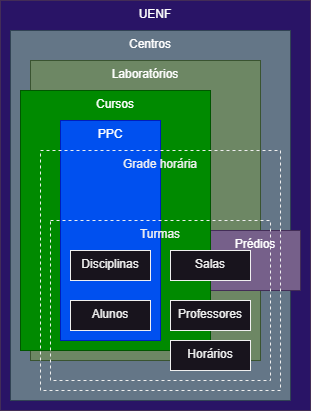
\includegraphics[width=0.5\textwidth]{files/img/2.02!3-instituicao/Diagramas Unificados-Euler-Relações entre as variáveis}
\end{MyCenteredFigure}

A \autoref{fig:relacoes} apresenta, na forma de um diagrama de Euler, a forma com a qual as variáveis presentes durante a criação da grade horária interagem entre si durante este processo. A figura, em conjunto com as descrições a seguir visam definir mais detalhadamente os termos utilizados na instituição estudada.

\begin{itemize}
  \item \textbf{Blocos/prédios}: são estruturas físicas que abrigam \textbf{salas} de aula. Cada bloco possui uma quantidade de salas, que são utilizadas para a realização das aulas;
  \item \textbf{Salas}: são estruturas físicas que abrigam as \textbf{turmas}. Cada sala possui uma capacidade máxima de \textbf{alunos}. Esse limite geralmente está atrelado à quantidade de carteiras disponíveis aos alunos, não sendo então necessariamente fixo, havendo geralmente a possibilidade de solicitar algumas carteiras de salas próximas. Elas estão teoricamente associadas aos \textbf{blocos}, visto que a compõem fisicamente, e são geridas pelos \textbf{centros}, que são responsáveis por distribuí-las. Na prática, algumas salas são preferencialmente utilizadas por determinados \textbf{cursos}, ficando então subgeridas pelos \textbf{laboratórios};
  \item \textbf{Centros}: são estruturas organizacionais que gerem os \textbf{laboratórios} e diversas \textbf{salas}. Embora cada \textbf{centro} geralmente esteja associado a um \textbf{bloco} específico, os centros não estão limitados a gerir as salas apenas deste bloco;
  \item \textbf{Laboratórios}: são estruturas organizacionais que englobam \textbf{professores}, \textbf{cursos}, \textbf{disciplinas} e \textbf{turmas}. Em sua maioria, os \textbf{laboratórios} estão associados a um único curso, entretanto, existem casos em que um laboratório está associado a mais de um curso, como é o caso do LCMAT, que está associado aos cursos de Matemática e de Ciência da Computação. Existe também o caso contrário, onde um curso está associado a mais de um laboratório, como é o do Bacharelado em Biologia que está associado a seis laboratórios;
  \item \textbf{Professores}: são aqueles que ministram as \textbf{disciplinas}. Teoricamente professor está vinculado a um \textbf{laboratório}, entretanto, na prática, os professores geralmente são associados aos \textbf{cursos} que geralmente ministram \textbf{disciplinas}. Teoricamente cada professor está passível de ministrar qualquer disciplina de seu laboratório, entretanto, na prática, os professores geralmente têm um conjunto de disciplinas que mais usualmente ministram;
  \item \textbf{Disciplinas}: um dos pontos principais na criação de uma \textbf{grade horária}. As \textbf{disciplinas} são ofertadas pelos \textbf{laboratórios} em \textbf{turmas}, que são alocadas em \textbf{salas} pelos \textbf{Centros}. Cada \textbf{PPC} define quais são as disciplinas e pré-requisitos que os \textbf{alunos} precisarão cursar. Uma mesma disciplina pode constar no PPC de diversos \textbf{cursos}. Cada disciplina possui uma carga horária, uma \textbf{ementa}, um nome e um código. Este código é composto por três letras, geralmente indicando o laboratório que o oferta, mas, em casos específicos, está associado a centros;
  \item \textbf{Turmas}: são a base da grade horária, ela consiste na representação da oferta de uma \textbf{disciplina} em um determinado \textbf{horário} e \textbf{sala}, com um determinado \textbf{professor} e para um determinado grupo de \textbf{alunos}. Mesmo que em sua maioria as disciplinas sejam ofertadas em apenas uma \textbf{turma}, existem casos em que uma disciplina é ofertada em mais de uma turma, nesses casos, um professor é atribuído como o coordenador de todas as turmas dessa disciplina. Situação essa que ocorre também com a atribuição de professores, havendo casos em que vários professores estão responsáveis por uma só turma; As turmas geralmente são direcionadas a \textbf{cursos} específicos, entretanto, existem casos em que uma turma é ofertada para mais de um curso simultaneamente;
  \item \textbf{Grade Horária}: é a representação de todas as \textbf{turmas} ofertadas em um determinado período letivo. A grade horária é composta por todas as \textbf{turmas} ofertadas, com seus respectivos \textbf{horários} e \textbf{salas}. A grade horária é a representação final do processo de criação de turmas. Esta representação geralmente é feita em formato de tabela e distribuída pelos \textbf{cursos} e \textbf{centros};
  \item \textbf{Horário}: ao se criar a \textbf{grade horária} é necessário alocar as \textbf{turmas} em um determinado momento de determinado dia da semana. Cada horário consiste de uma hora de início e uma duração (ou hora de término). Geralmente as turmas que são oferecidas aos \textbf{cursos} seguem o turno respectivo do curso, mesmo que às vezes fuja deste padrão. As turmas em sua maioria são distribuídas em horários de 2 horas com um espaço de um dia entre elas, entretanto, existem casos em que as turmas possuem 3 horas de duração. Os horários disponíveis para alocação são das 7 às 22 horas;
  \item \textbf{Cursos}: são estruturas organizacionais nos quais os \textbf{alunos} estão matriculados. Cada curso possui um turno no qual as suas turmas são ofertadas, esses turnos podem ser matutino, vespertino ou noturno;
  \item \textbf{Projeto Pedagógico do Curso (PPC)}: é o documento que define a estrutura curricular do \textbf{curso}, contendo as \textbf{disciplinas} obrigatórias, optativas e eletivas, bem como a quantidade de créditos necessários para a conclusão do curso;
  \item \textbf{Alunos}: são aqueles que frequentam as \textbf{turmas}. Cada \textbf{aluno} geralmente está vinculado ao PPC vigente para seu \textbf{curso} no ano de sua matrícula, havendo casos em que se é permitida a mudança de PPC. Segundo o PPC estão definidas quais são as \textbf{disciplinas} que o aluno deve cursar para integralizar o curso.
\end{itemize}

\chapter{Desenvolvimento do sistema de suporte à decisão} \label{chap:desenvolvimento}  % ##   5

Este capítulo visa apresentar todo o processo realizado para o desenvolvimento do sistema de suporte à decisão. O propósito desta aplicação é auxiliar o coordenador do curso de Ciência da Computação da UENF na alocação interativa de turmas, professores e salas. O auxílio é dado através de duas formas: a primeira é a \hyperref[par:Solução inicial]{criação automatizada da grade baseada no histórico das grades anteriores}, a segunda é a \hyperref[sec:conflitos]{identificação de conflitos}, como a alocação de uma turma grande demais para a capacidade da sala, com o objetivo de auxiliar no aprimoramento da grade inicialmente gerada.

Inicia-se com a apresentação de \hyperref[sec:projetos]{projetos anteriores} que serviram de base para o desenvolvimento do presente trabalho. Em seguida, será apresentado o \hyperref[sec:LGPD]{acesso aos dados acadêmicos da instituição} e as dificuldades encontradas para a sua obtenção. Posteriormente, será apresentado o processo de \hyperref[sec:prototipagem]{prototipagem} do sistema, onde foram criados os designs iniciais das telas do sistema. Em seguida, será apresentado o processo de \hyperref[sec:programação]{programação do sistema}, que foi dividido em três grandes categorias que visavam entregar o sistema de forma gradual e funcional.

Por fim, será apresentado o cerne do sistema que é a \hyperref[sec:conflitos]{identificação e visualização de conflitos}, ou seja, os casos em que a alocação dos recursos gera algum comportamento minimamente indesejável como por exemplo a alocação de uma sala a duas turmas ao mesmo tempo. Serão apresentados os tipos de conflitos que o sistema é capaz de identificar, como eles são visualizados e como o sistema lida com cada um deles. Conclui-se então com a apresentação do \hyperref[sec:preenchimento]{preenchimento do banco de dados} com dados reais.

\section{Projetos anteriores} \label{sec:projetos}                                      % ###  5.1

Antes do desenvolvimento do presente trabalho, outros projetos já foram idealizados e até mesmo desenvolvidos. Dentre eles, dois se destacam por terem sido os precursores do atual projeto. O primeiro deles, que foi idealizado, mas não desenvolvido, almejava apresentar uma \hyperref[ssec:andamento]{visualização da progressão dos alunos na grade curricular}. O segundo, que foi desenvolvido, realizava o \hyperref[ssec:demanda]{cálculo da demanda}, ou seja, calculava quantos e quais eram os alunos que poderiam se inscrever nas disciplinas. Ambos os projetos se mostram como abordagens paralelas de auxiliar no planejamento do curso de Ciência da Computação da UENF, sendo eles também sistemas de suporte à decisão, mesmo que em menor escala.

Deve-se comentar também sobre os dois trabalhos anteriores desenvolvidos por \citeonline{SanyaSantos2013} e \citeonline{RicardoSilveira2014} que iniciaram os estudos sobre a alocação de turmas no curso de Ciência da Computação na UENF, que foram \hyperref[sec:anteriores]{citados previamente}.

\subsection{Andamento dos alunos} \label{ssec:andamento}                                % #### 5.1.1

% Como interesse próprio, c
Cogitou-se o desenvolvimento de uma plataforma onde se pudesse ver em que ponto os alunos se encontram em relação à grade curricular de seus cursos. Para isso, seria necessária a obtenção dos dados dos alunos, seja por parte dos mesmos, do coordenador ou por integração com o sistema acadêmico. Com estes dados, seria possível criar uma interface que mostrasse o andamento dos alunos, quais matérias já foram cursadas, quais estão sendo cursadas e quais ainda faltam. Além disso, seria possível mostrar quais matérias são pré-requisitos para outras. Assim, o aluno e a coordenação poderiam ter uma visão geral de seu andamento e de quais matérias ele precisará cursar para se formar.
% Esse projeto não saiu do mundo das ideias, entretanto, lá permaneceu sendo maturado.

\begin{MyCenteredFigure} \caption{Andamento do aluno no Sistema Acadêmico} \label{fig:andamento}
  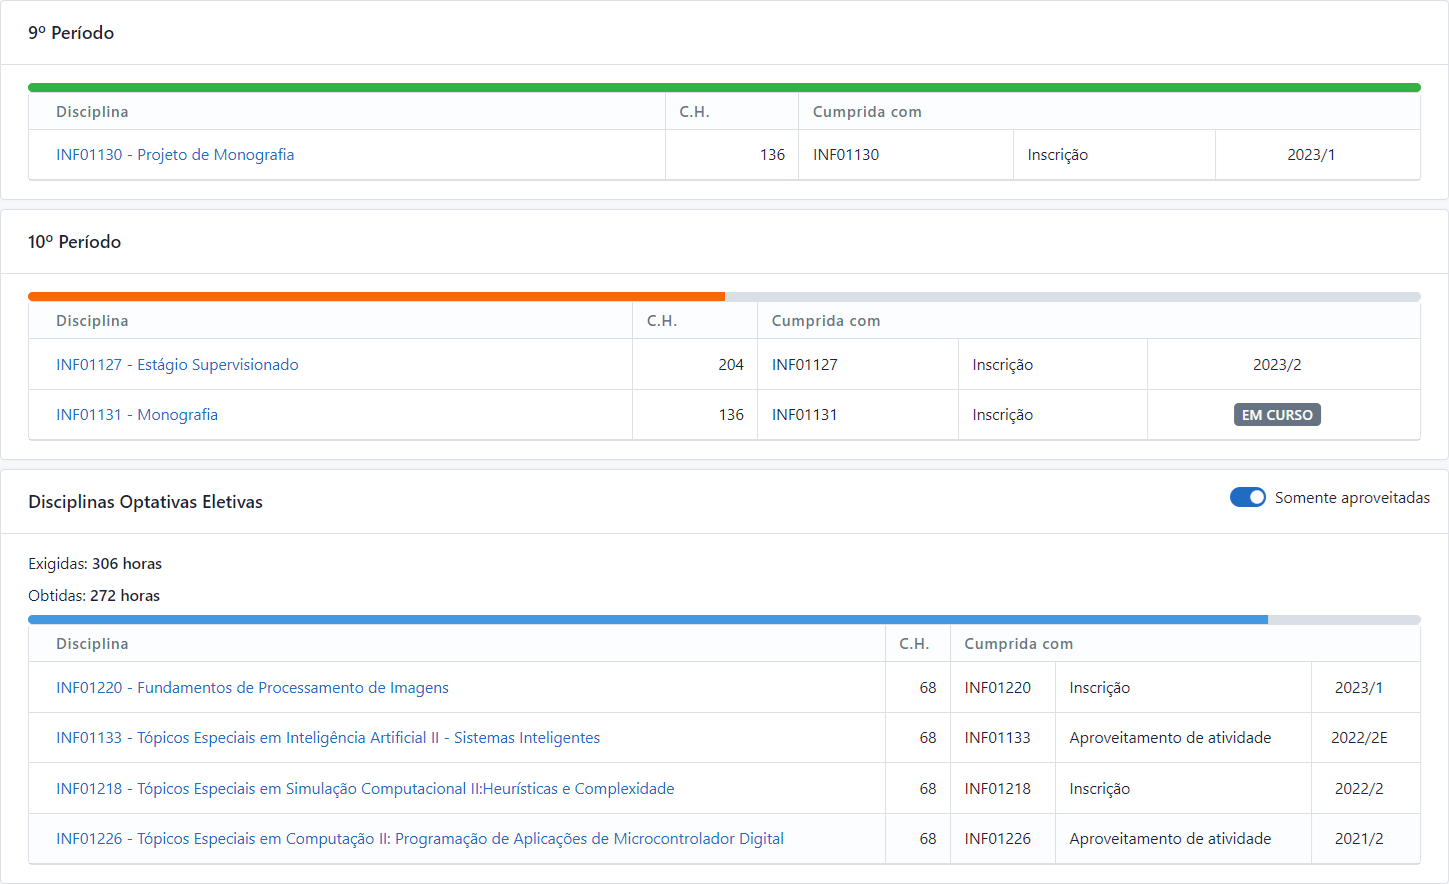
\includegraphics[width=\textwidth]{files/img/2.02!5-desenvolvimento/2.02!5.1-anteriores/Progressão}
\end{MyCenteredFigure}

Anos após a concepção dessa funcionalidade, o Sistema Acadêmico da UENF passou a disponibilizar uma funcionalidade semelhante, como pode ser visto na \autoref{fig:andamento}. Nela, é possível ver o andamento do aluno por período, incluindo as disciplinas Eletivas Livres e Eletivas Optativas. Entretanto, essa visualização tabular não ilustra o andamento de todos os alunos simultaneamente, sendo necessário navegar individualmente por cada um deles.

\subsection{Cálculo de demanda} \label{ssec:demanda}                                    % #### 5.1.2

Durante o intervalo entre os semestres, os alunos precisam se inscrever nas matérias que desejam cursar no semestre seguinte. Para isso, é necessário que o coordenador saiba quantos alunos estão interessados em cada matéria para que ele possa definir quantas turmas serão abertas. Com este fim em mente, o coordenador dispõe de algumas alternativas como estimar quantos alunos se inscreverão em cada disciplina, checar manualmente no sistema acadêmico quais alunos podem fazer cada matéria, ou então obter diretamente dos alunos através de um formulário em quais disciplinas cada um dos alunos tem a intenção de cursar.

O método que o atual Coordenador de Ciência da Computação utiliza consiste em baixar o extrato de todos os alunos do curso e tabelar no Excel qual é o andamento de cada um dos alunos, para que assim, através da análise manual, pudesse ver qual é o andamento de cada um e quantos alunos demandam quais disciplinas.

Entretanto, todas essas alternativas são trabalhosas e propensas a erros. Sendo assim, foi pensado em uma forma de automatizar esse processo. Foi então elaborado um código em \LinkToURL{\LinkPython}{Python} que atualmente \LinkToURL{\LinkProjetoDemanda}{se encontra no GitHub}. Este código tem como entrada os extratos de matrícula dos alunos e como saída a listagem das disciplinas demandadas e a listagem dos alunos que demandam cada disciplina.

\lstinputlisting[language={Python}, captionpos={t}, label={code:demand}, caption={Obter demanda por extratos em PDF}]{files/codigos/demanda.py}

Este código foi desenvolvido em 8 etapas, vistas no \autoref{code:demand}, cada uma com um arquivo separado. Para alcançar a lista das demandas, é necessário primeiro obter a lista dos arquivos em formato PDF que serão processados, em seguida extrair seus dados com a biblioteca \LinkToURL{\LinkPDFMiner}{\textit{PDFMiner}}, estruturar os dados obtidos, filtrar os dados estruturados, obter a demanda de cada disciplina, juntar as demandas de cada disciplina e salvar os dados obtidos em um arquivo de texto.

Embora o código cumpra com seu objetivo, apresenta algumas características limitantes. A primeira é que os PDFs precisam ser obtidos manualmente, um por um, pelo coordenador, sendo ela por si só uma tarefa extenuante, o que não é desejado. Além disso, o seu uso não é muito intuitivo, sendo necessário que o usuário lide com o prompt de comando e instale as dependências necessárias, o que acaba trazendo uma dificuldade a mais ao usuário. O código também apresenta limitações por sistema operacional, não sendo garantido o seu funcionamento em sistemas operacionais diferentes do Windows.

\section{Acesso aos dados acadêmicos da instituição} \label{sec:LGPD}                   % ###  5.2

Em sua concepção original, o presente trabalho visaria integrar o sistema desenvolvido com o atual sistema acadêmico da UENF. Essa abordagem foi descartada devido às dificuldades encontradas por parte do setor administrativo da UENF que, devido à \LinkToURL{\LinkLGPD}{Lei Geral de Proteção dos Dados (LGPD)}, não podem divulgar dados dos alunos, mesmo anonimizados.

Para confirmação das informações recebidas, a LGPD foi estudada e cogitou-se que o presente estudo pudesse estar amparado pela alínea b do inciso 2º do artigo 4º do capítulo 1 da Lei Nº 13.709, de 14 de agosto de 2018. Informando este que esta lei, a LGPD, não se aplica ao tratamento de dados pessoais realizado para fins exclusivamente acadêmicos. Segundo o \LinkToURL{\LinkLGPDEstudoTécnico}{Estudo Técnico sobre o tratamento de dados pessoais para fins acadêmicos}, é reforçado que ``o tratamento de dados pessoais para fins acadêmicos deve ser sempre lícito''.

Apesar das possibilidades de meios legalmente válidos para a aquisição dos dados, optou-se por abandonar a integração com o Sistema Acadêmico e o uso de dados reais dos alunos já existentes na plataforma. Rumando-se então para uma abordagem de inserção manual de dados por parte dos usuários do sistema.

\section{Prototipagem} \label{sec:prototipagem}                                         % ###  5.3

A criação de protótipos, seguindo a abordagem tomada por \citeonline{Andre2018}, se mostra como essencial para que se mantenha a constante satisfação por parte dos \textit{stakeholders}. Isso se dá com o intuito de saber quais mudanças eles sugerem ao desenvolvimento do projeto, assim reduzindo a necessidade de retrabalho e de não alcançar as expectativas do projeto. Para este fim, foram feitos os designs iniciais das telas do sistema usando o software de design \LinkToURL{\LinkFigma}{Figma}, designs esses que representam apenas o esboço, e não um sistema funcional. Esse esboço serviu como uma base visual de como o sistema estaria no final.

\subsection{Protótipos de componentes} \label{ssec:componentes}                         % #### 5.3.1

Antes de seguir com a descrição das telas, é válido descrever os componentes que foram utilizados na construção dos protótipos. Os componentes principais são os cartões de turma (\autoref{fig:cartão_de_turma}) e as caixas de seleção (\autoref{fig:selects}).

A \autoref{fig:cartão_de_turma} mostra os cartões de turma que foram utilizados para representar as turmas criadas. O objetivo desses cartões é de apresentar de forma compacta o máximo possível de informações relevantes ao usuário. Considerando o caráter iterativo do desenvolvimento, foram criados diversas versões dos cartões, todos eles visando a apresentação de informações de forma clara, objetiva e intuitiva por parte do usuário.

Essas informações relevantes são as informações relacionadas à identificação da disciplina, do professor e da sala. Além dessas, são apresentadas informações adicionais como a quantidade de alunos que podem se inscrever na disciplina e alertas de possíveis conflitos. Em todas as versões dos cartões de turma, o código da disciplina está no canto superior esquerdo. No canto inferior direito está a quantidade de alunos que podem se inscrever na disciplina e, à sua esquerda, aqueles alunos que apresentam algum tipo de impedimento, como por exemplo ter alguma outra turma que ele possa se inscrever no mesmo horário.

\begin{MyCenteredFigure} \caption{Protótipos de cartões de turma} \label{fig:cartão_de_turma}
  \begin{subfigure}[b]{0.45\textwidth} \centering
    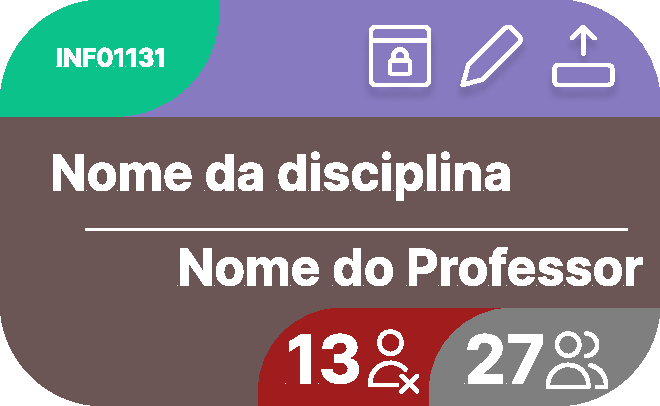
\includegraphics[width=\textwidth]{files/img/2.02!5-desenvolvimento/2.02!5.3-prototipagem/5.3.1-componentes/Cartões/PadraoClassCards}
    \caption{Turma padrão} \label{fig:TurmaPadrão}
  \end{subfigure}
  \hfill
  \begin{subfigure}[b]{0.45\textwidth} \centering
    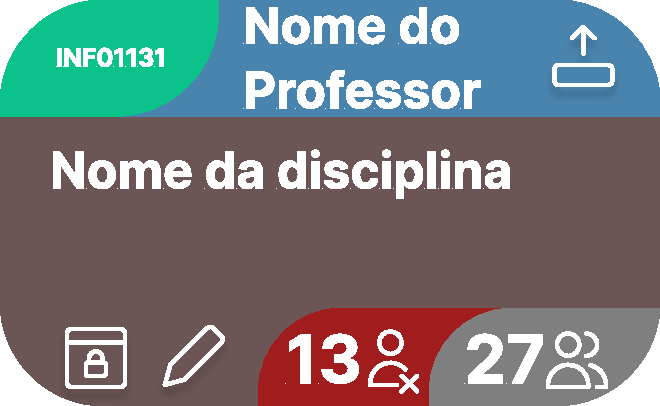
\includegraphics[width=\textwidth]{files/img/2.02!5-desenvolvimento/2.02!5.3-prototipagem/5.3.1-componentes/Cartões/Professor SuperiorClassCards}
    \caption{Turma com professor no topo} \label{fig:TurmaTopo}
  \end{subfigure}

  \begin{subfigure}[b]{0.45\textwidth} \centering
    
\includegraphics[width=\textwidth]{files/img/2.02!5-desenvolvimento/2.02!5.3-prototipagem/5.3.1-componentes/Cartões/Smaller ColapsadaClassCards}
    \caption{Turma colapsadas} \label{fig:TurmaColapsada}
  \end{subfigure}
  \hfill
  \begin{subfigure}[b]{0.45\textwidth} \centering
    
\includegraphics[width=\textwidth]{files/img/2.02!5-desenvolvimento/2.02!5.3-prototipagem/5.3.1-componentes/Cartões/SmallestClassCards}
    \caption{Turma com tamanho reduzido} \label{fig:TurmaColapsadaReduzida}
  \end{subfigure}
\end{MyCenteredFigure}

Nestes cartões, estão presentes também três botões: \textbf{travar}, \textbf{editar} e \textbf{expandir}/\textbf{recolher}. O botão de \textbf{travar} tem como função fixar a turma no horário em que ela se encontra, impedindo que ela seja movida. O botão de \textbf{editar} tem como função abrir um painel onde é possível alterar as informações da turma. O botão de \textbf{expandir}/\textbf{recolher} tem como função expandir ou recolher o cartão, mostrando ou escondendo informações adicionais. Em cada uma das versões dos cartões, a posição dos botões foram alteradas.

Outras informaçõe que também tiveram sua posição alterada foram o nome do professor, o nome da disciplina e o código da sala.

Cada uma dessas versões dos cartões de turma se mostra com um propósito específico. O cartão padrão (\autoref{fig:TurmaPadrão}) é um dos maiores cartões, o que facilita a visualização do usuário às informações importantes, o mesmo pode ser dito para o cartão com o professor no topo (\autoref{fig:TurmaTopo}), esse, por sua vez, distribui a posição dos botões. Já os botões colapsados (\autoref{fig:TurmaColapsada}) e o cartão com tamanho reduzido (\autoref{fig:TurmaColapsadaReduzida}) prezam por uma maior economia de espaço, sendo úteis para quando o usuário deseja visualizar mais turmas ao mesmo tempo, como é o caso da visualização da grade horária, e por isso informam também o código da sala em que estão alocados.

\begin{MyCenteredFigure} \caption{Protótipos de caixas de seleção} \label{fig:selects}
  \begin{subfigure}[b]{0.45\textwidth} \centering
    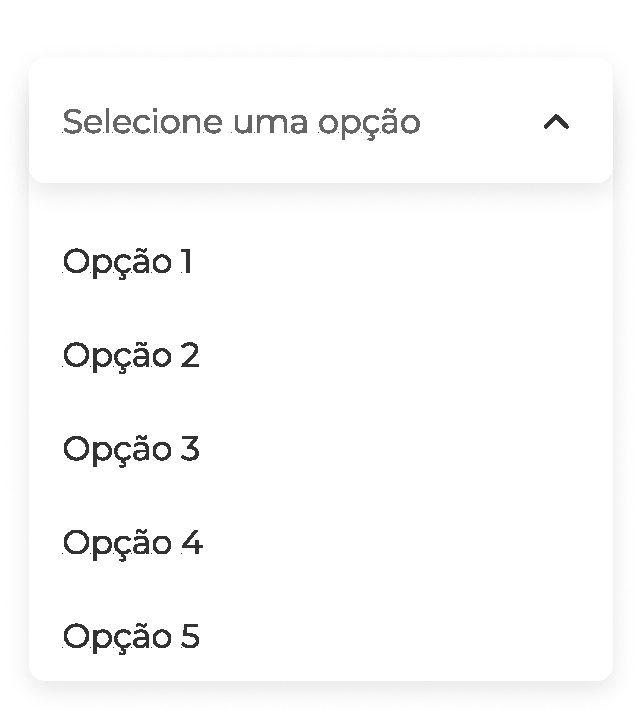
\includegraphics[width=0.8\textwidth]{files/img/2.02!5-desenvolvimento/2.02!5.3-prototipagem/5.3.1-componentes/SingleSelect}
    \caption{Caixa de seleção única} \label{fig:SingleSelect}
  \end{subfigure}
  \hfill
  \begin{subfigure}[b]{0.45\textwidth} \centering
    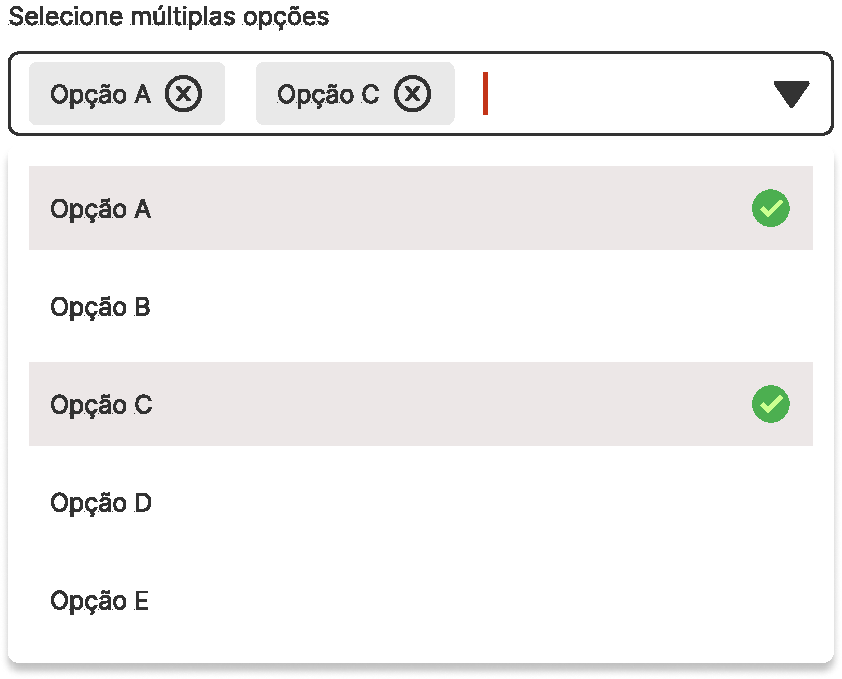
\includegraphics[width=\textwidth]{files/img/2.02!5-desenvolvimento/2.02!5.3-prototipagem/5.3.1-componentes/MultiSelect}
    \caption{Caixa de seleção múltipla} \label{fig:MultiSelect}
  \end{subfigure}
\end{MyCenteredFigure}

A \autoref{fig:selects} mostra os protótipos de caixas de seleção que foram utilizados para a seleção de dados. Na \autoref{fig:SingleSelect} está a caixa de seleção onde o usuário pode selecionar apenas uma opção. Já na \autoref{fig:MultiSelect} a caixa de seleção permite ao usuário selecionar várias opções.

\subsection{Protótipos de páginas} \label{ssec:páginas}                                 % #### 5.3.2

Aqui serão elencadas as sete páginas esboçadas para o sistema. Sendo elas a \hyperref[fig:main]{página principal} (\autoref{fig:main}), a \hyperref[fig:CRUD_main]{página de seleção} (\autoref{fig:CRUD_main}), a \hyperref[fig:CRUD_salas]{página de salas} (\autoref{fig:CRUD_salas}), a \hyperref[fig:CRUD_alunos]{página de alunos} (\autoref{fig:CRUD_alunos}), a \hyperref[fig:CRUD_disciplinas]{página de disciplinas} (\autoref{fig:CRUD_disciplinas}), a \hyperref[fig:CRUD_professores]{página de professores} (\autoref{fig:CRUD_professores}) e a \hyperref[fig:CRUD_turmas]{página de turmas} (\autoref{fig:CRUD_turmas}).

A \textbf{primeira página} é a ilustrada pela \autoref{fig:main} que permite que o usuário arraste todas as turmas listadas até o horário desejado. A listagem das turmas a serem distribuídas é disposta em um painel à esquerda. Este painel tem como funcionalidade, fixar as turmas ainda não alocadas, como se estivessem presas por \LinkToURL{\LinkVelcro}{fechos de gancho e laço}. Assim, dispondo de um local para que turmas em processo de mudança de horário sejam armazenadas temporariamente sem que sejam perdidas.

\begin{MyCenteredFigure} \caption{Protótipo da página principal do sistema} \label{fig:main}
  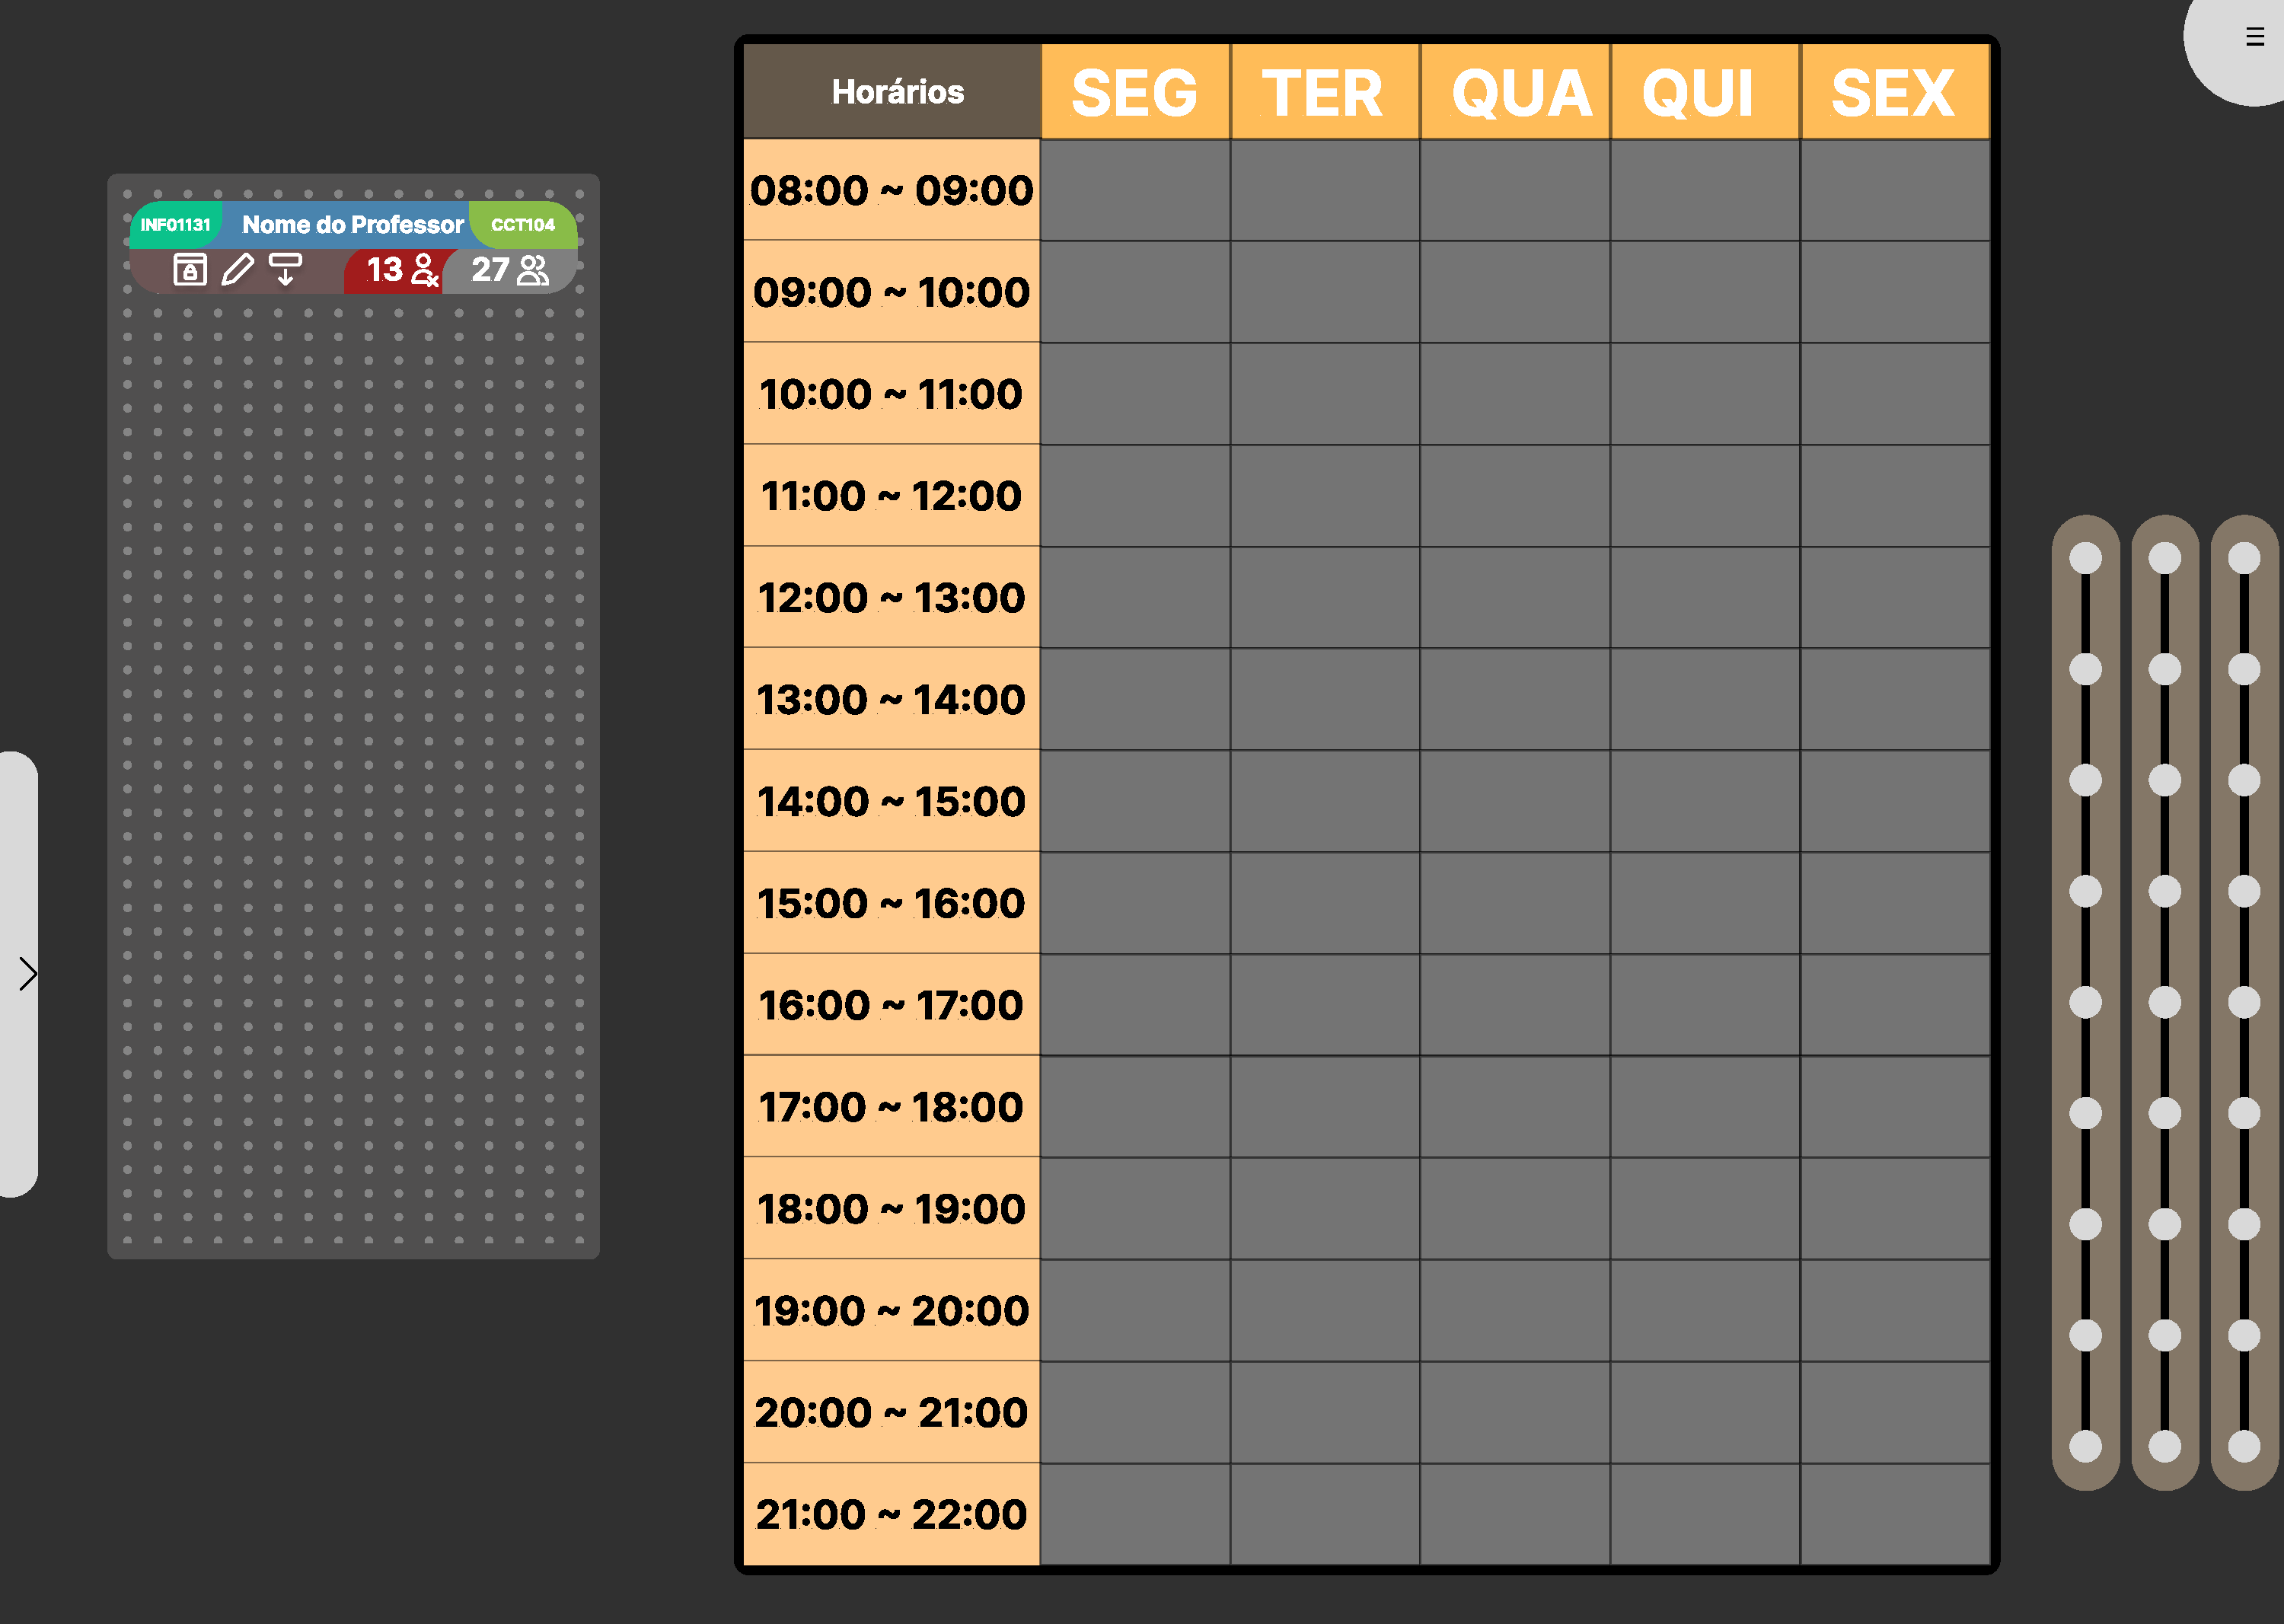
\includegraphics[width=\textwidth]{files/img/2.02!5-desenvolvimento/2.02!5.3-prototipagem/5.3.2-paginas/1-main}
\end{MyCenteredFigure}

Em seguida, temos a \textbf{página de seleção} (\autoref{fig:CRUD_main}) da categoria dos dados que deseja-se modificar, podendo esses serem sobre os professores, alunos, salas, disciplinas ou turmas. Cada uma destas tendo a capacidade de criação, leitura, edição e deleção dos dados.

\begin{MyCenteredFigure} \caption{Protótipo da página de seleção} \label{fig:CRUD_main}
  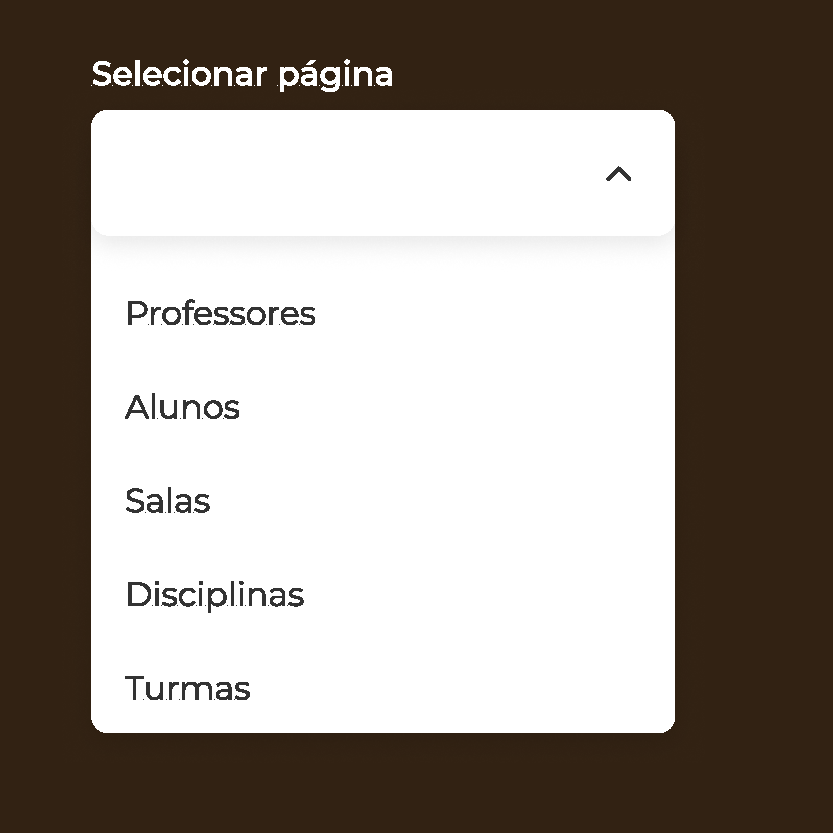
\includegraphics[width=0.5\textwidth]{files/img/2.02!5-desenvolvimento/2.02!5.3-prototipagem/5.3.2-paginas/2-CRUD_main}
\end{MyCenteredFigure}

Quanto à \textbf{página das salas} (\autoref{fig:CRUD_salas}), temos primeiro a seleção da sala na qual deseja-se fazer alterações de cadastro. Abaixo desta caixa de seleção única há um filtro de visualização das alocações de determinado ano e semestre. Nessa página pode-se também registrar algumas características da sala, como a quantidade de cadeiras e computadores, e se possui monitor, projetos, quadro de giz e quadro branco. Um exemplo de sala ainda sem turmas alocadas é representado na \autoref{fig:CRUD_salas}. Essas últimas informações, embora não sejam essenciais para a alocação das turmas, podem ser úteis como forma de filtragem para a alocação de turmas, visto que certas disciplinas demandam salas com características específicas.

\begin{MyCenteredFigure} \caption{Protótipo da página de salas} \label{fig:CRUD_salas}
  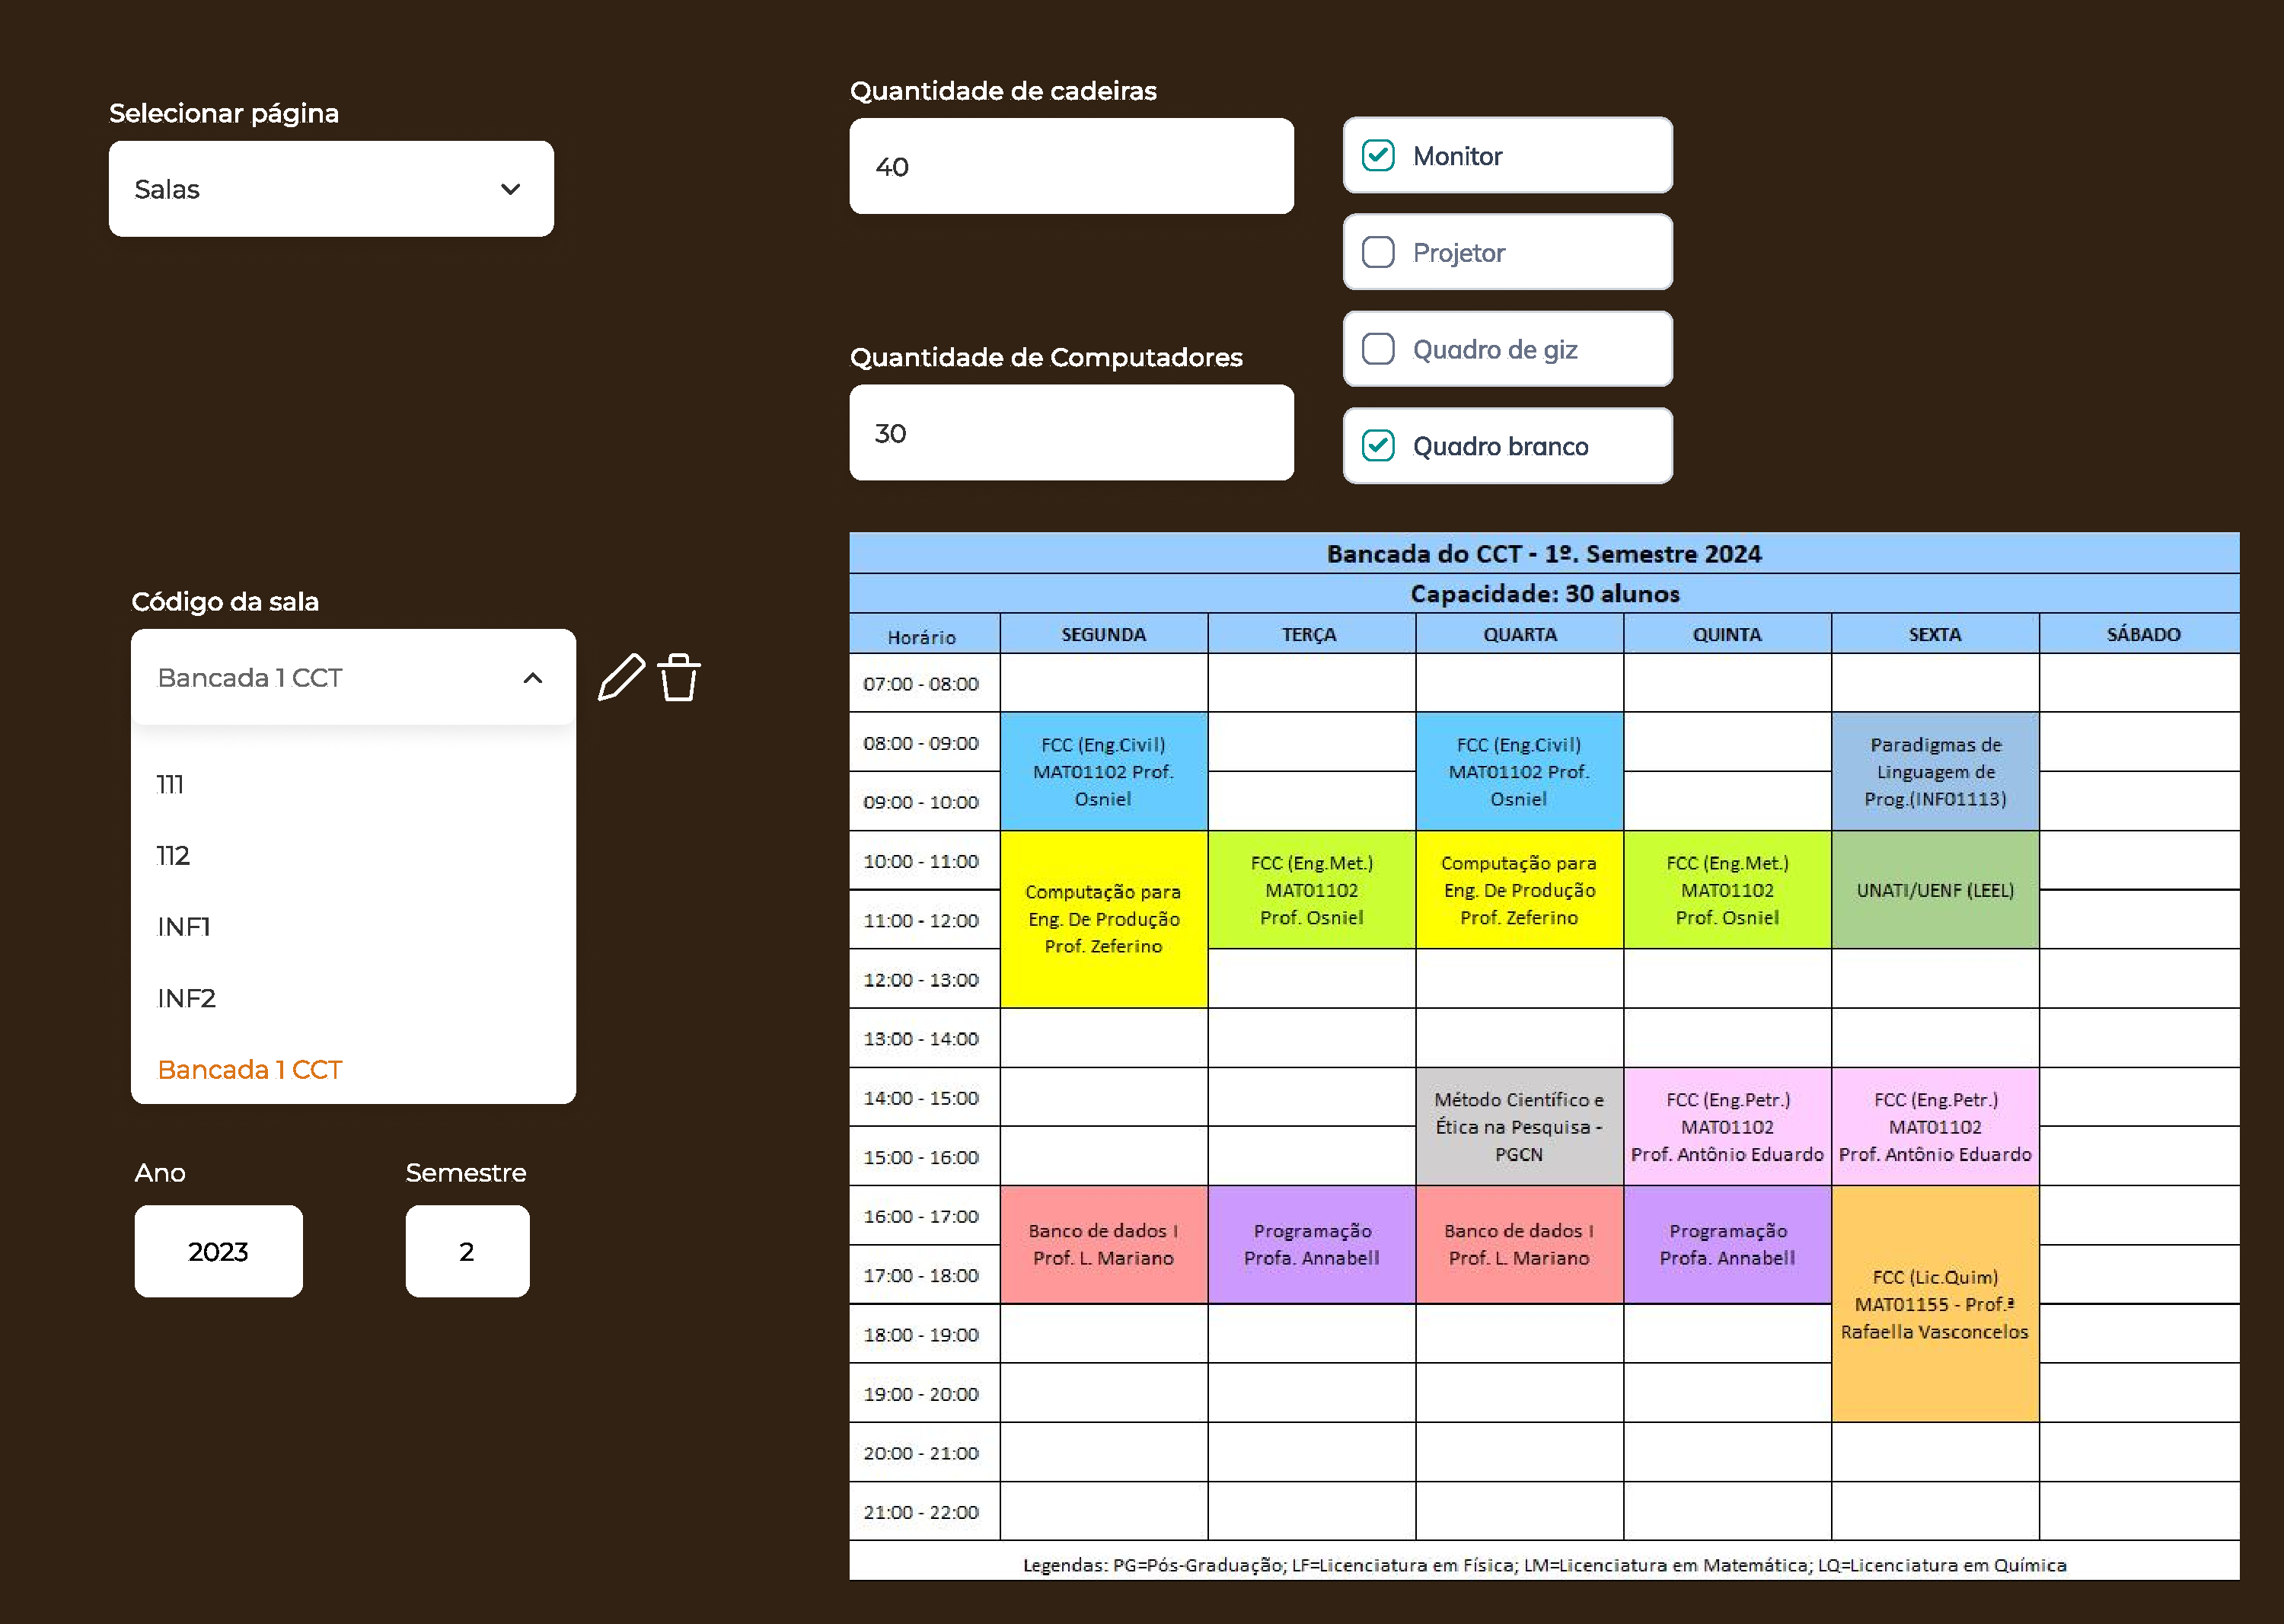
\includegraphics[width=0.9\textwidth]{files/img/2.02!5-desenvolvimento/2.02!5.3-prototipagem/5.3.2-paginas/3-CRUD_salas}
\end{MyCenteredFigure}

Na \textbf{página dos alunos}, pode-se cadastrar novos alunos informando o seu ano de entrada e a sua matrícula. Abaixo temos a visualização da grade, onde pode-se classificar cada uma das disciplinas como aprovada, reprovada e cursando. O exemplo da \autoref{fig:CRUD_alunos} mostra a grade de um aluno inscrito em 2019.1.

\begin{MyCenteredFigure} \caption{Protótipo da página de alunos} \label{fig:CRUD_alunos}
  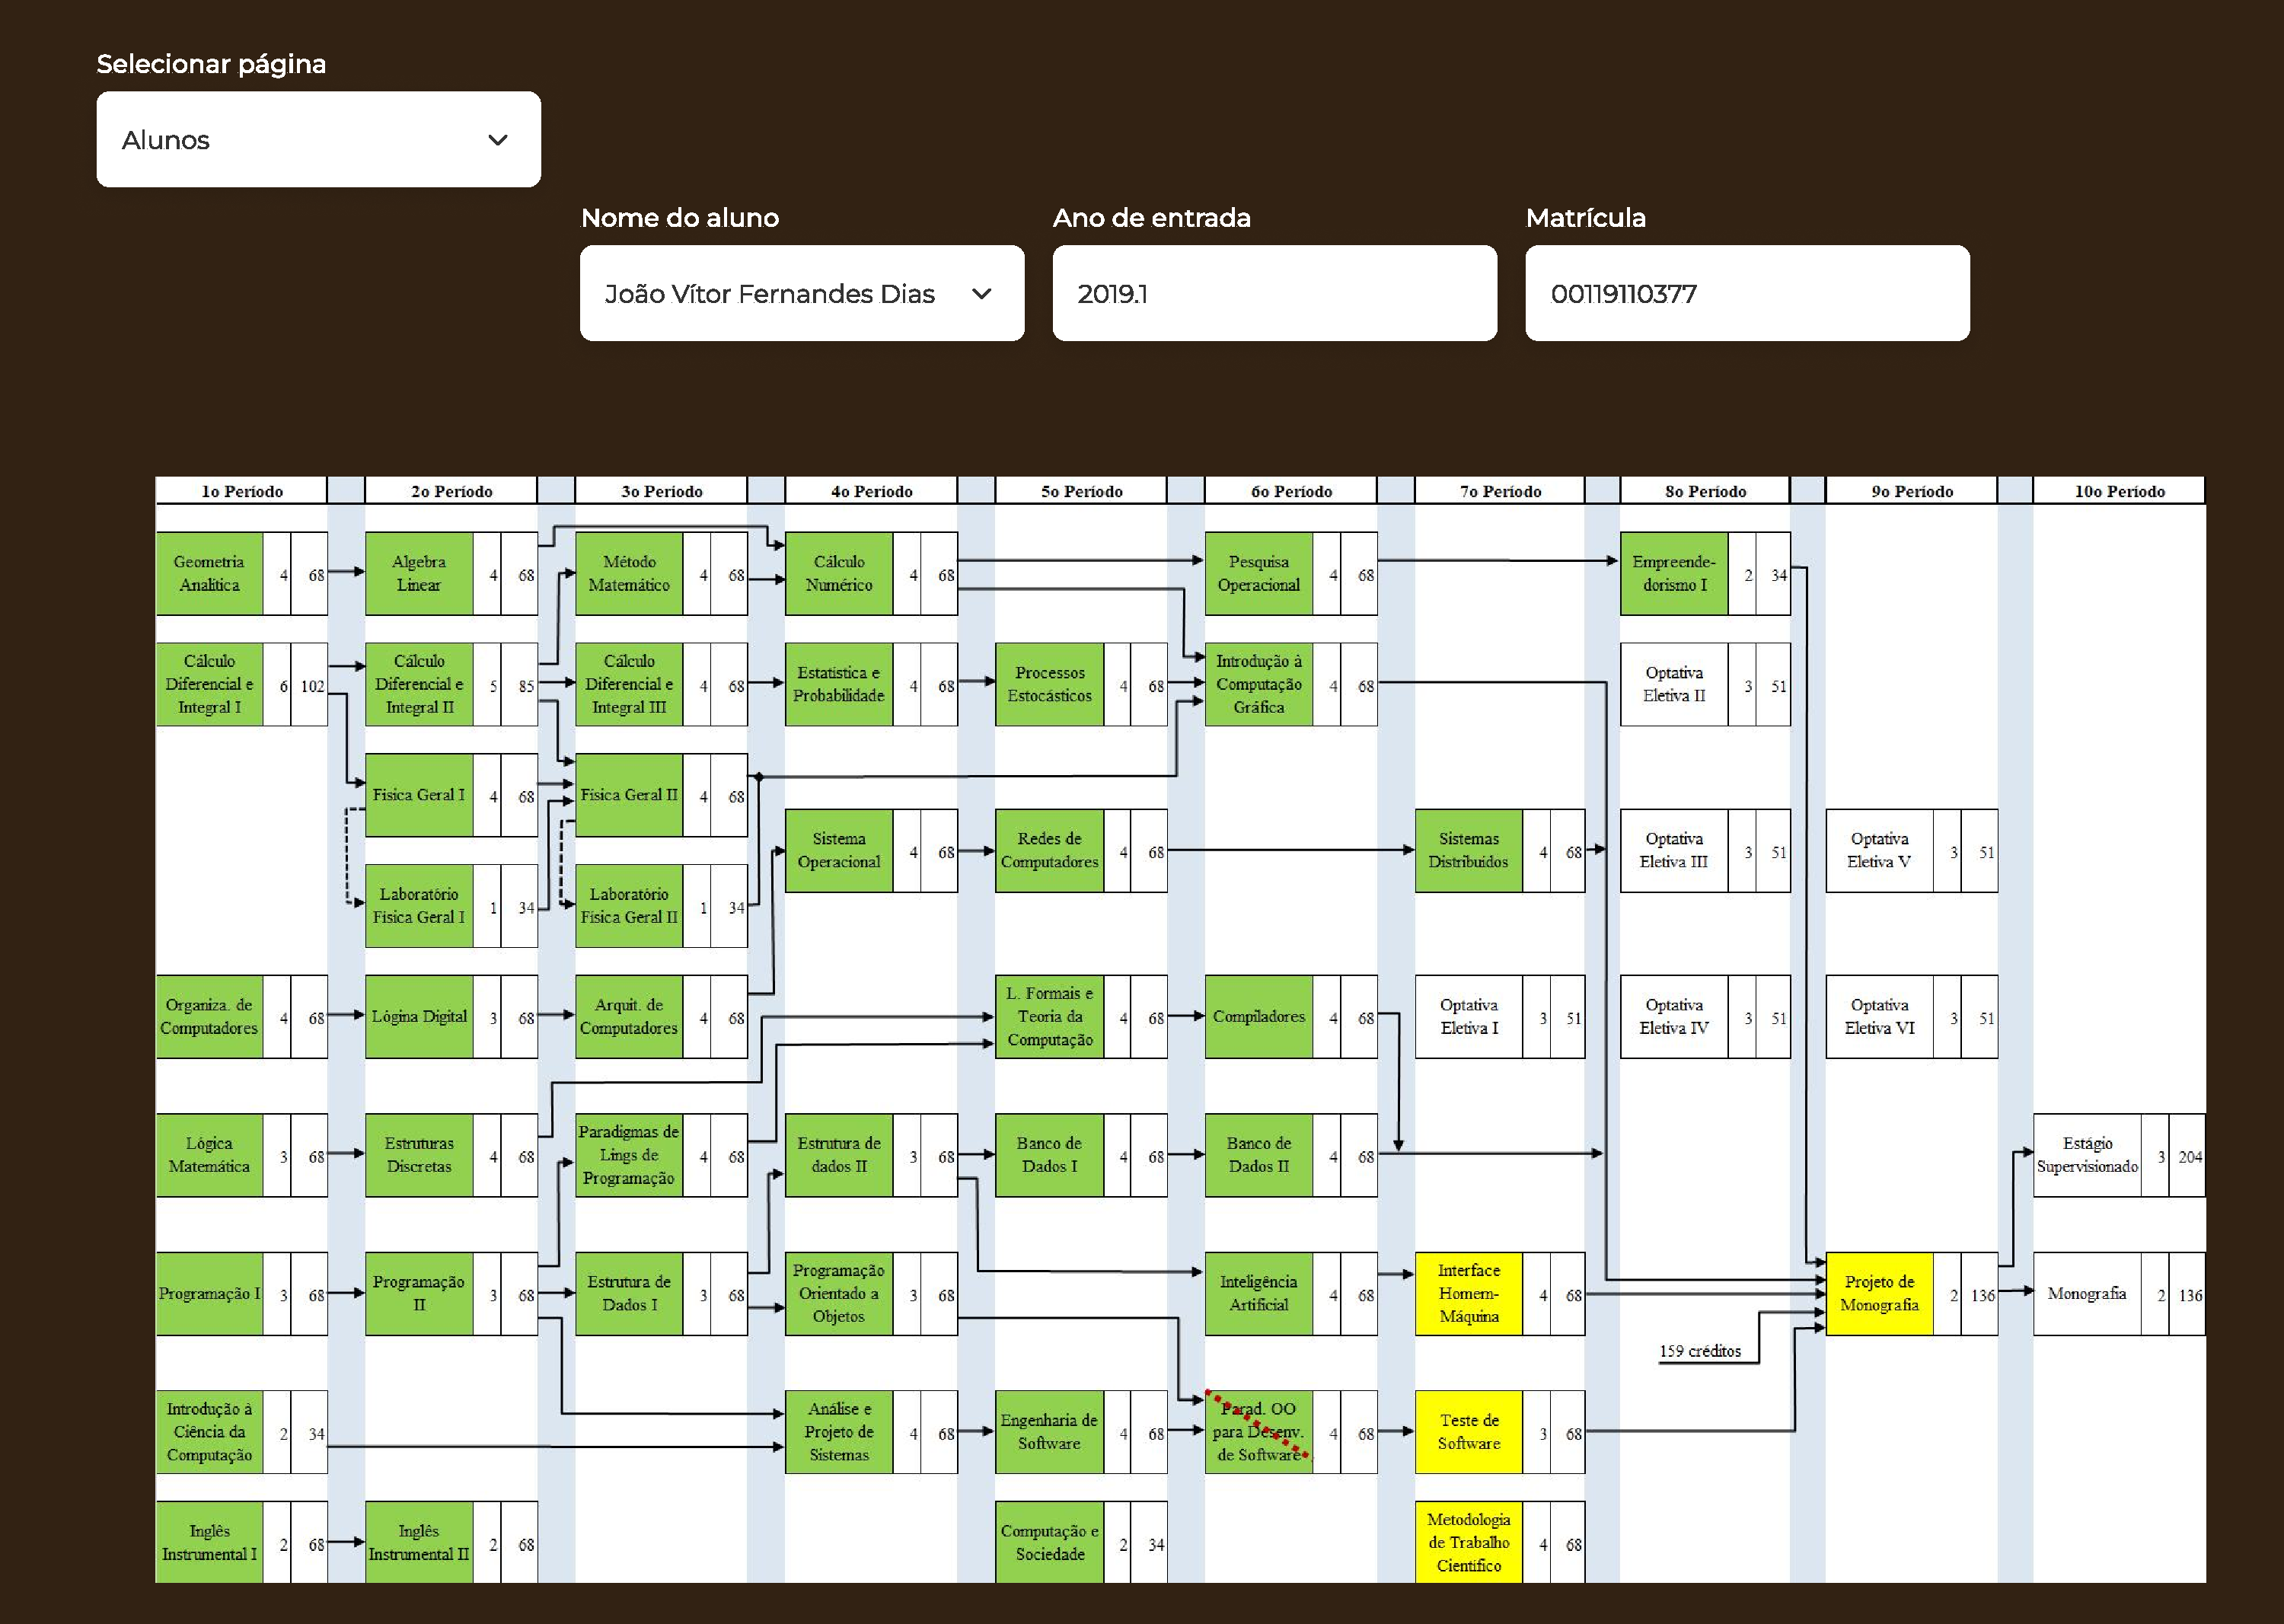
\includegraphics[width=0.9\textwidth]{files/img/2.02!5-desenvolvimento/2.02!5.3-prototipagem/5.3.2-paginas/4-CRUD_alunos}
\end{MyCenteredFigure}

Podemos definir na \textbf{página das disciplinas} qual seu código, nome, e o seu período esperado segundo a matriz curricular. Além dessas informações, pode-se cadastrar quais cursos a possuem em suas matrizes curriculares, quais seus pré-requisitos, os professores que a ministram e quais requisitos a mesma possui em relação às características de sala. A \autoref{fig:CRUD_disciplinas} mostra a página de modificação de disciplinas.

\begin{MyCenteredFigure} \caption{Protótipo da página de disciplinas} \label{fig:CRUD_disciplinas}
  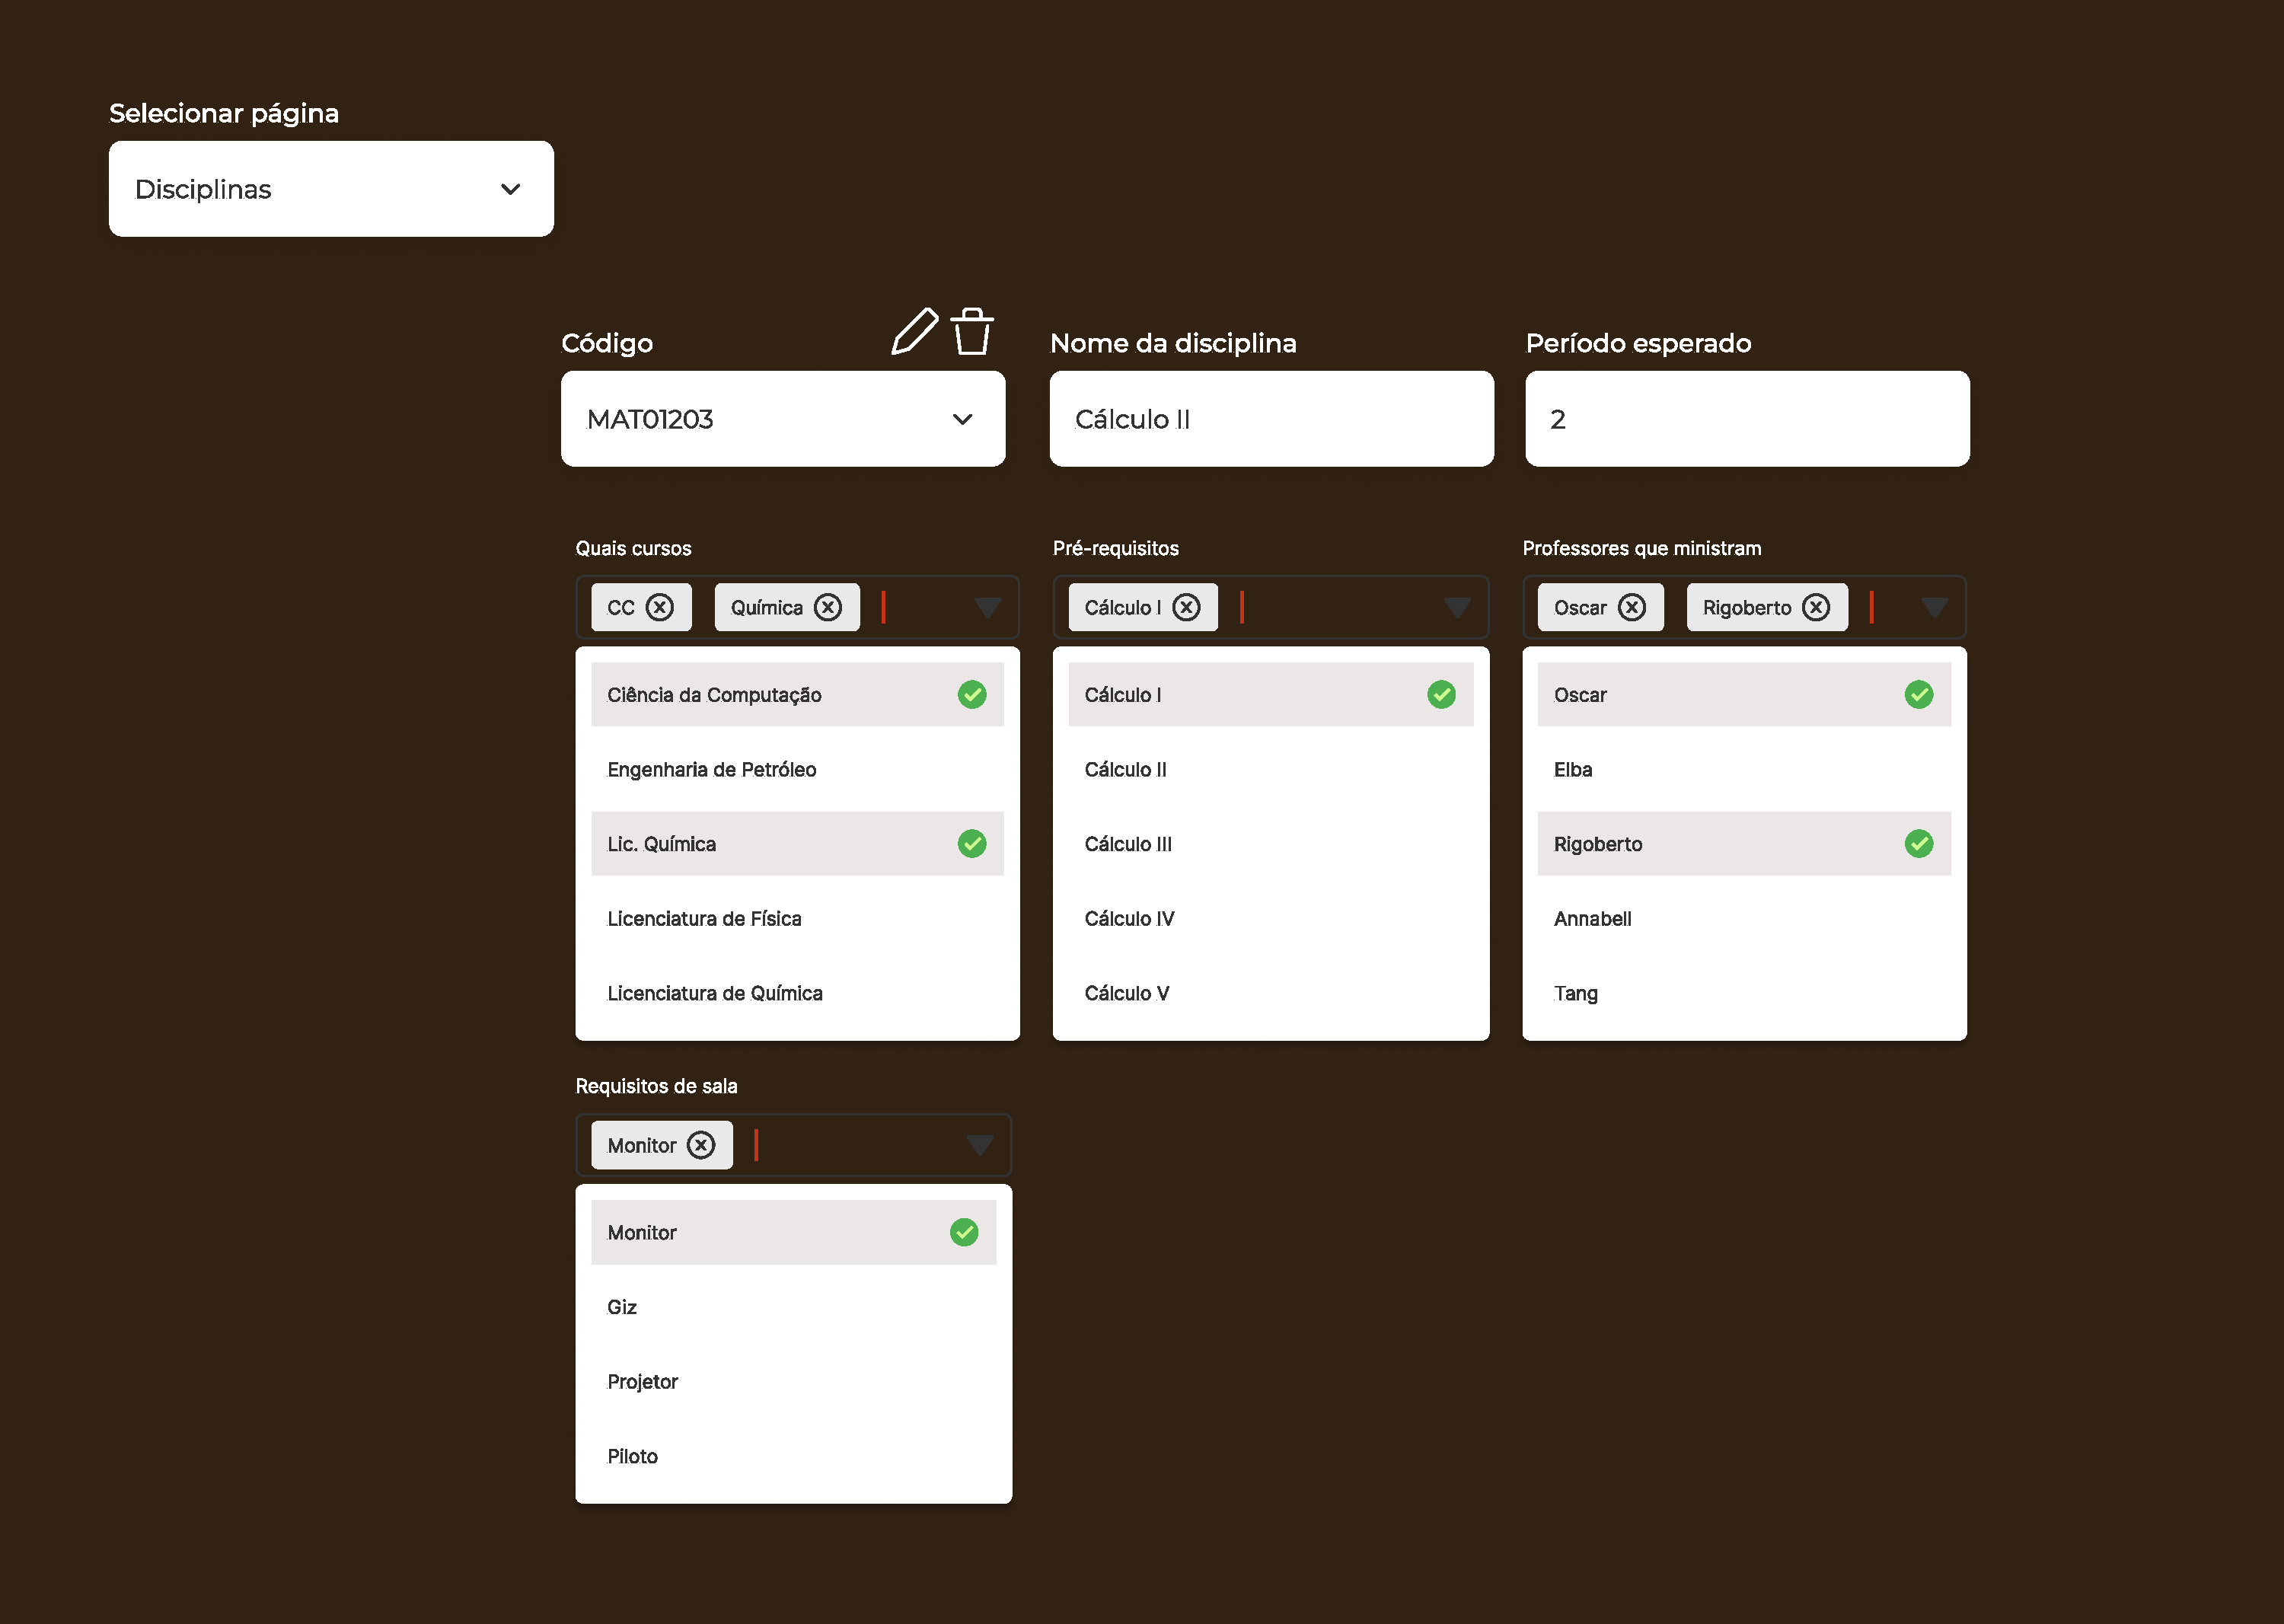
\includegraphics[width=0.8\textwidth]{files/img/2.02!5-desenvolvimento/2.02!5.3-prototipagem/5.3.2-paginas/5-CRUD_disciplinas}
\end{MyCenteredFigure}

Na \textbf{página de professores} (\autoref{fig:CRUD_professores}), temos a relação de disciplinas que os mesmos estão passíveis de ministrar, e também quais são suas preferências de horários ao longo da semana. Embora não seja essencial, essa informação pode ser útil para a alocação de turmas, pois alguns professores podem ter preferência, ou até mesmo não estarem disponíveis para ministrar aulas em determinados horários. Um exemplo deste caso seriam os bolsistas de apoio ao ensino, dado que os mesmos podem estar também vinculados a outras instituições. E nesses casos, aquele que estiver desenvolvendo a grade horária pode alocar as turmas de acordo com a disponibilidade dos professores.

\begin{MyCenteredFigure} \caption{Protótipo da página de professores} \label{fig:CRUD_professores}
  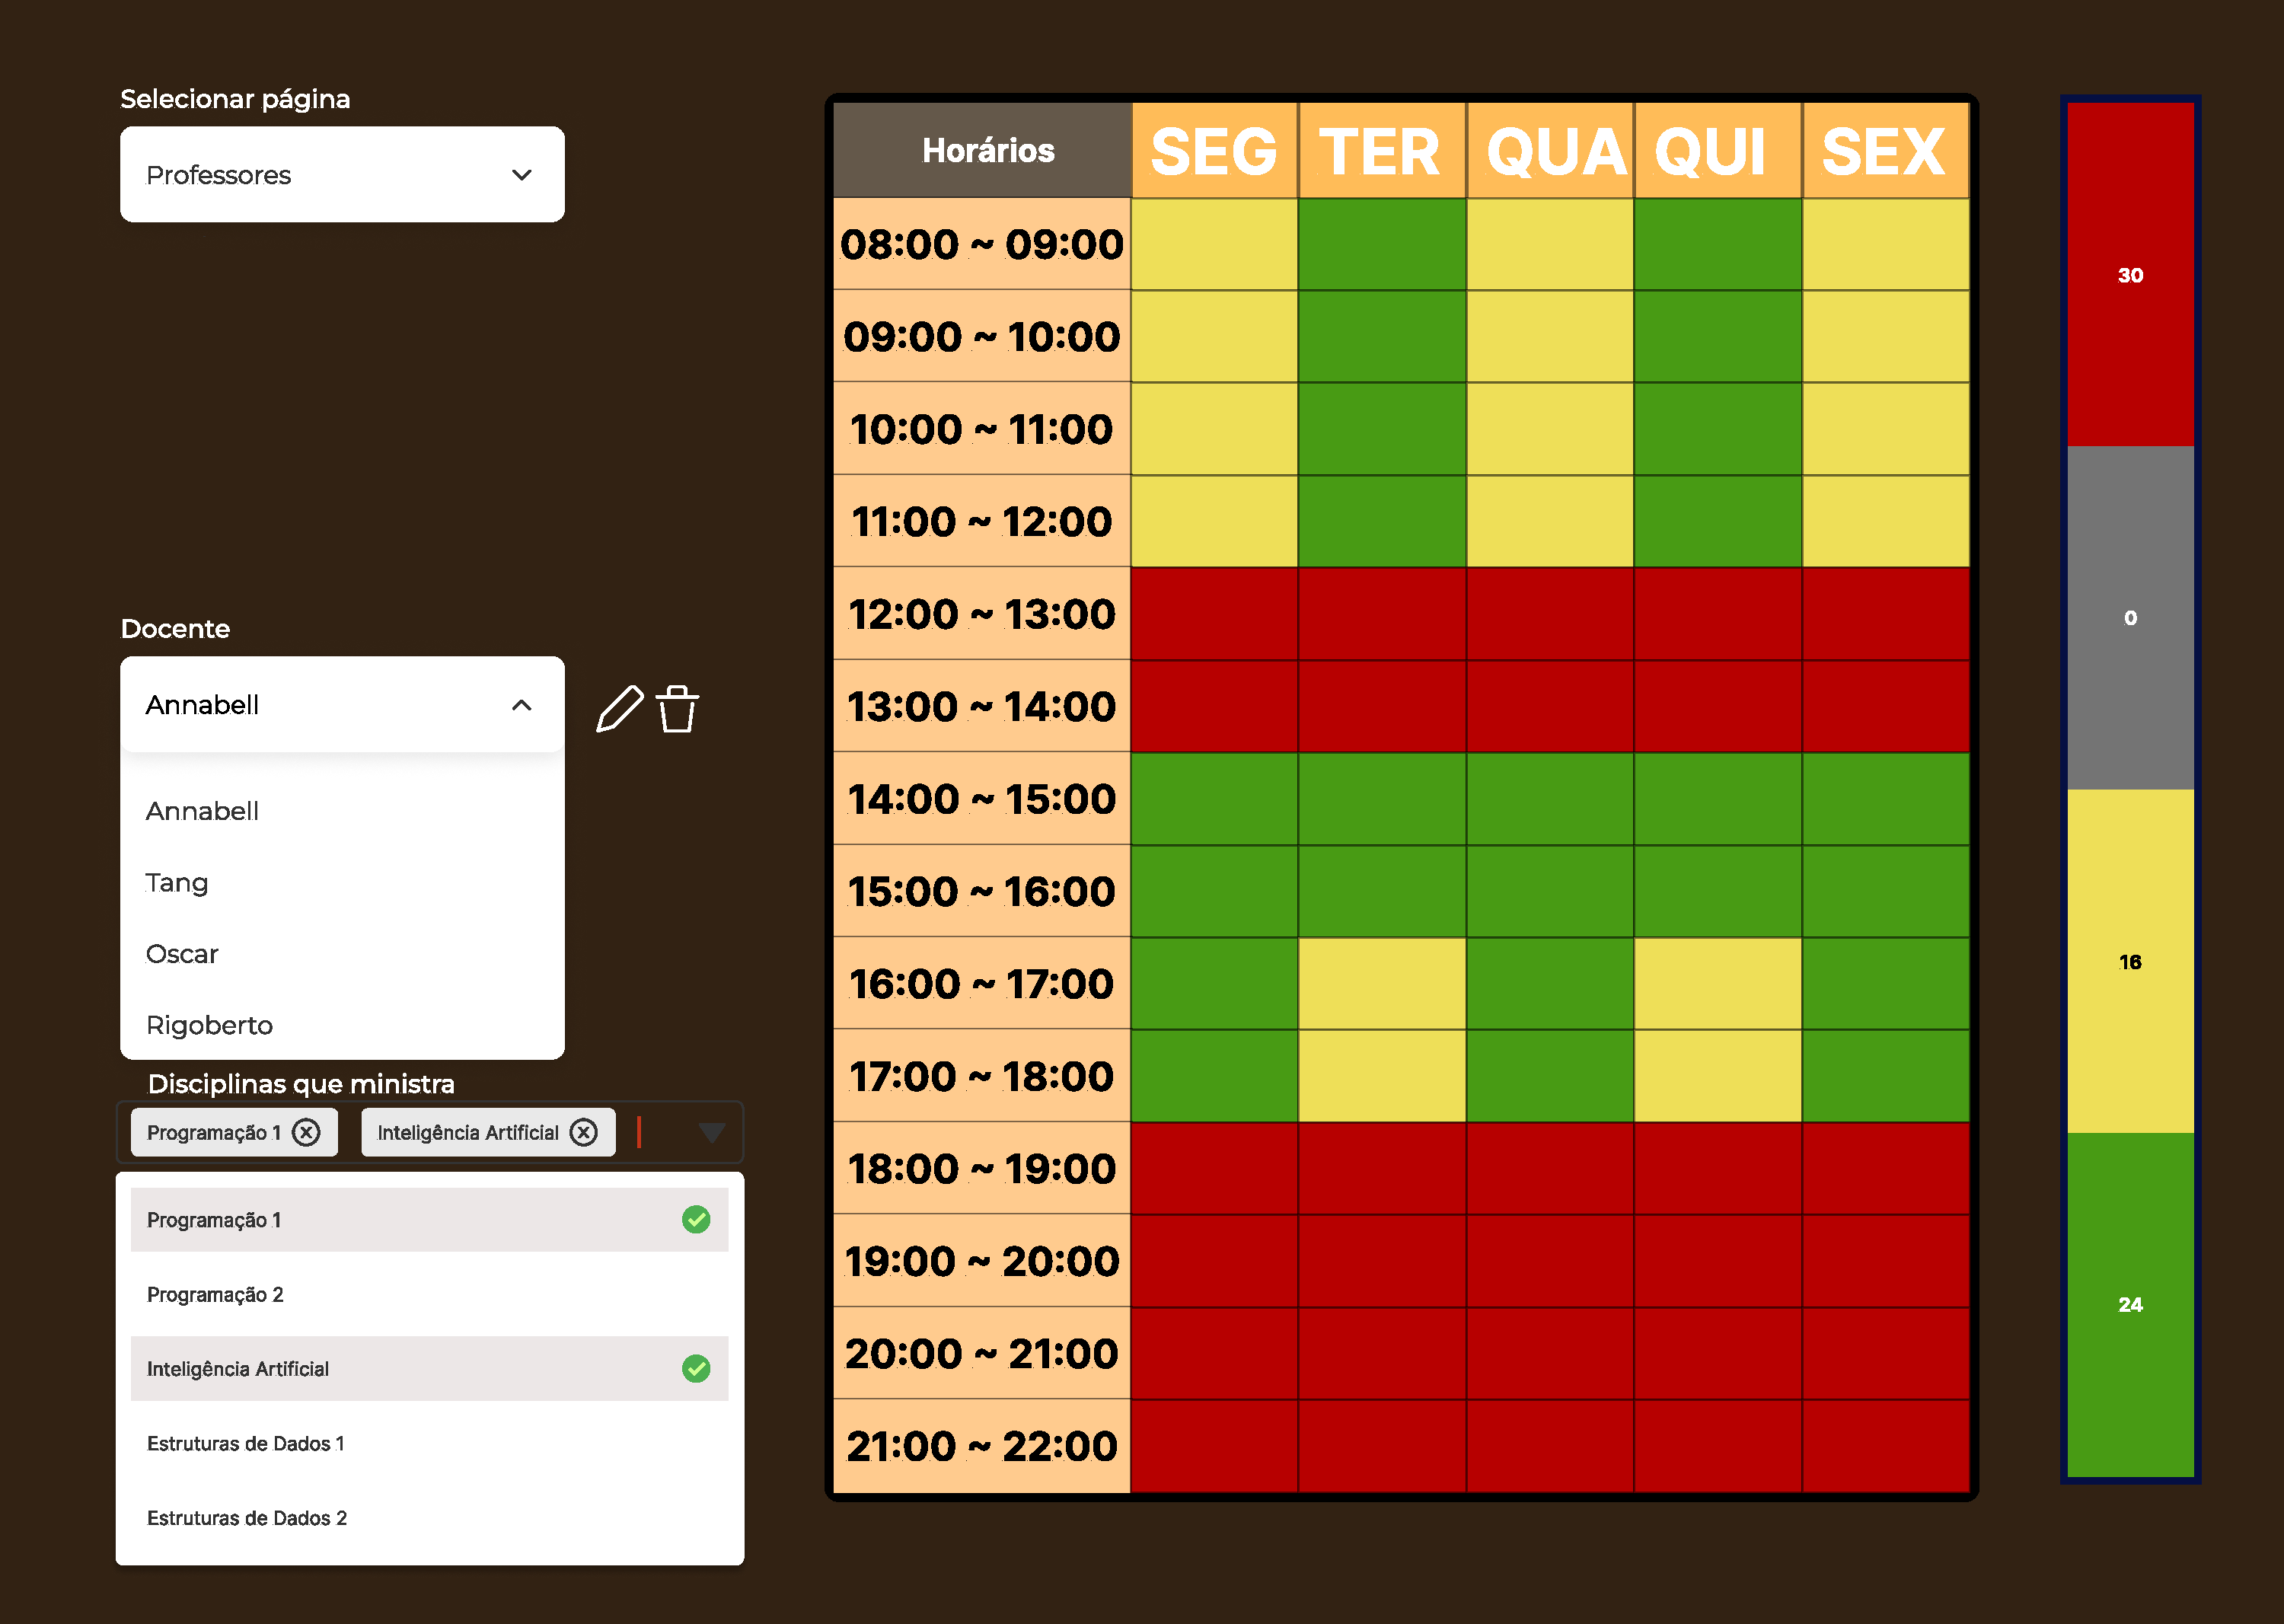
\includegraphics[width=0.8\textwidth]{files/img/2.02!5-desenvolvimento/2.02!5.3-prototipagem/5.3.2-paginas/6-CRUD_professores}
\end{MyCenteredFigure}

Por fim, na \autoref{fig:CRUD_turmas}, temos a junção de todas as informações registradas acima. Nela, podemos alocar os seus horários, definindo o ano, semestre, dia, hora de início e duração em que será ministrada. Também é necessário que seja definido em que sala cada um de seus horários estará alocada. Além de informar, também, qual professor a lecionará e a qual disciplina ela se refere.

\begin{MyCenteredFigure} \caption{Protótipo da página de turmas} \label{fig:CRUD_turmas}
  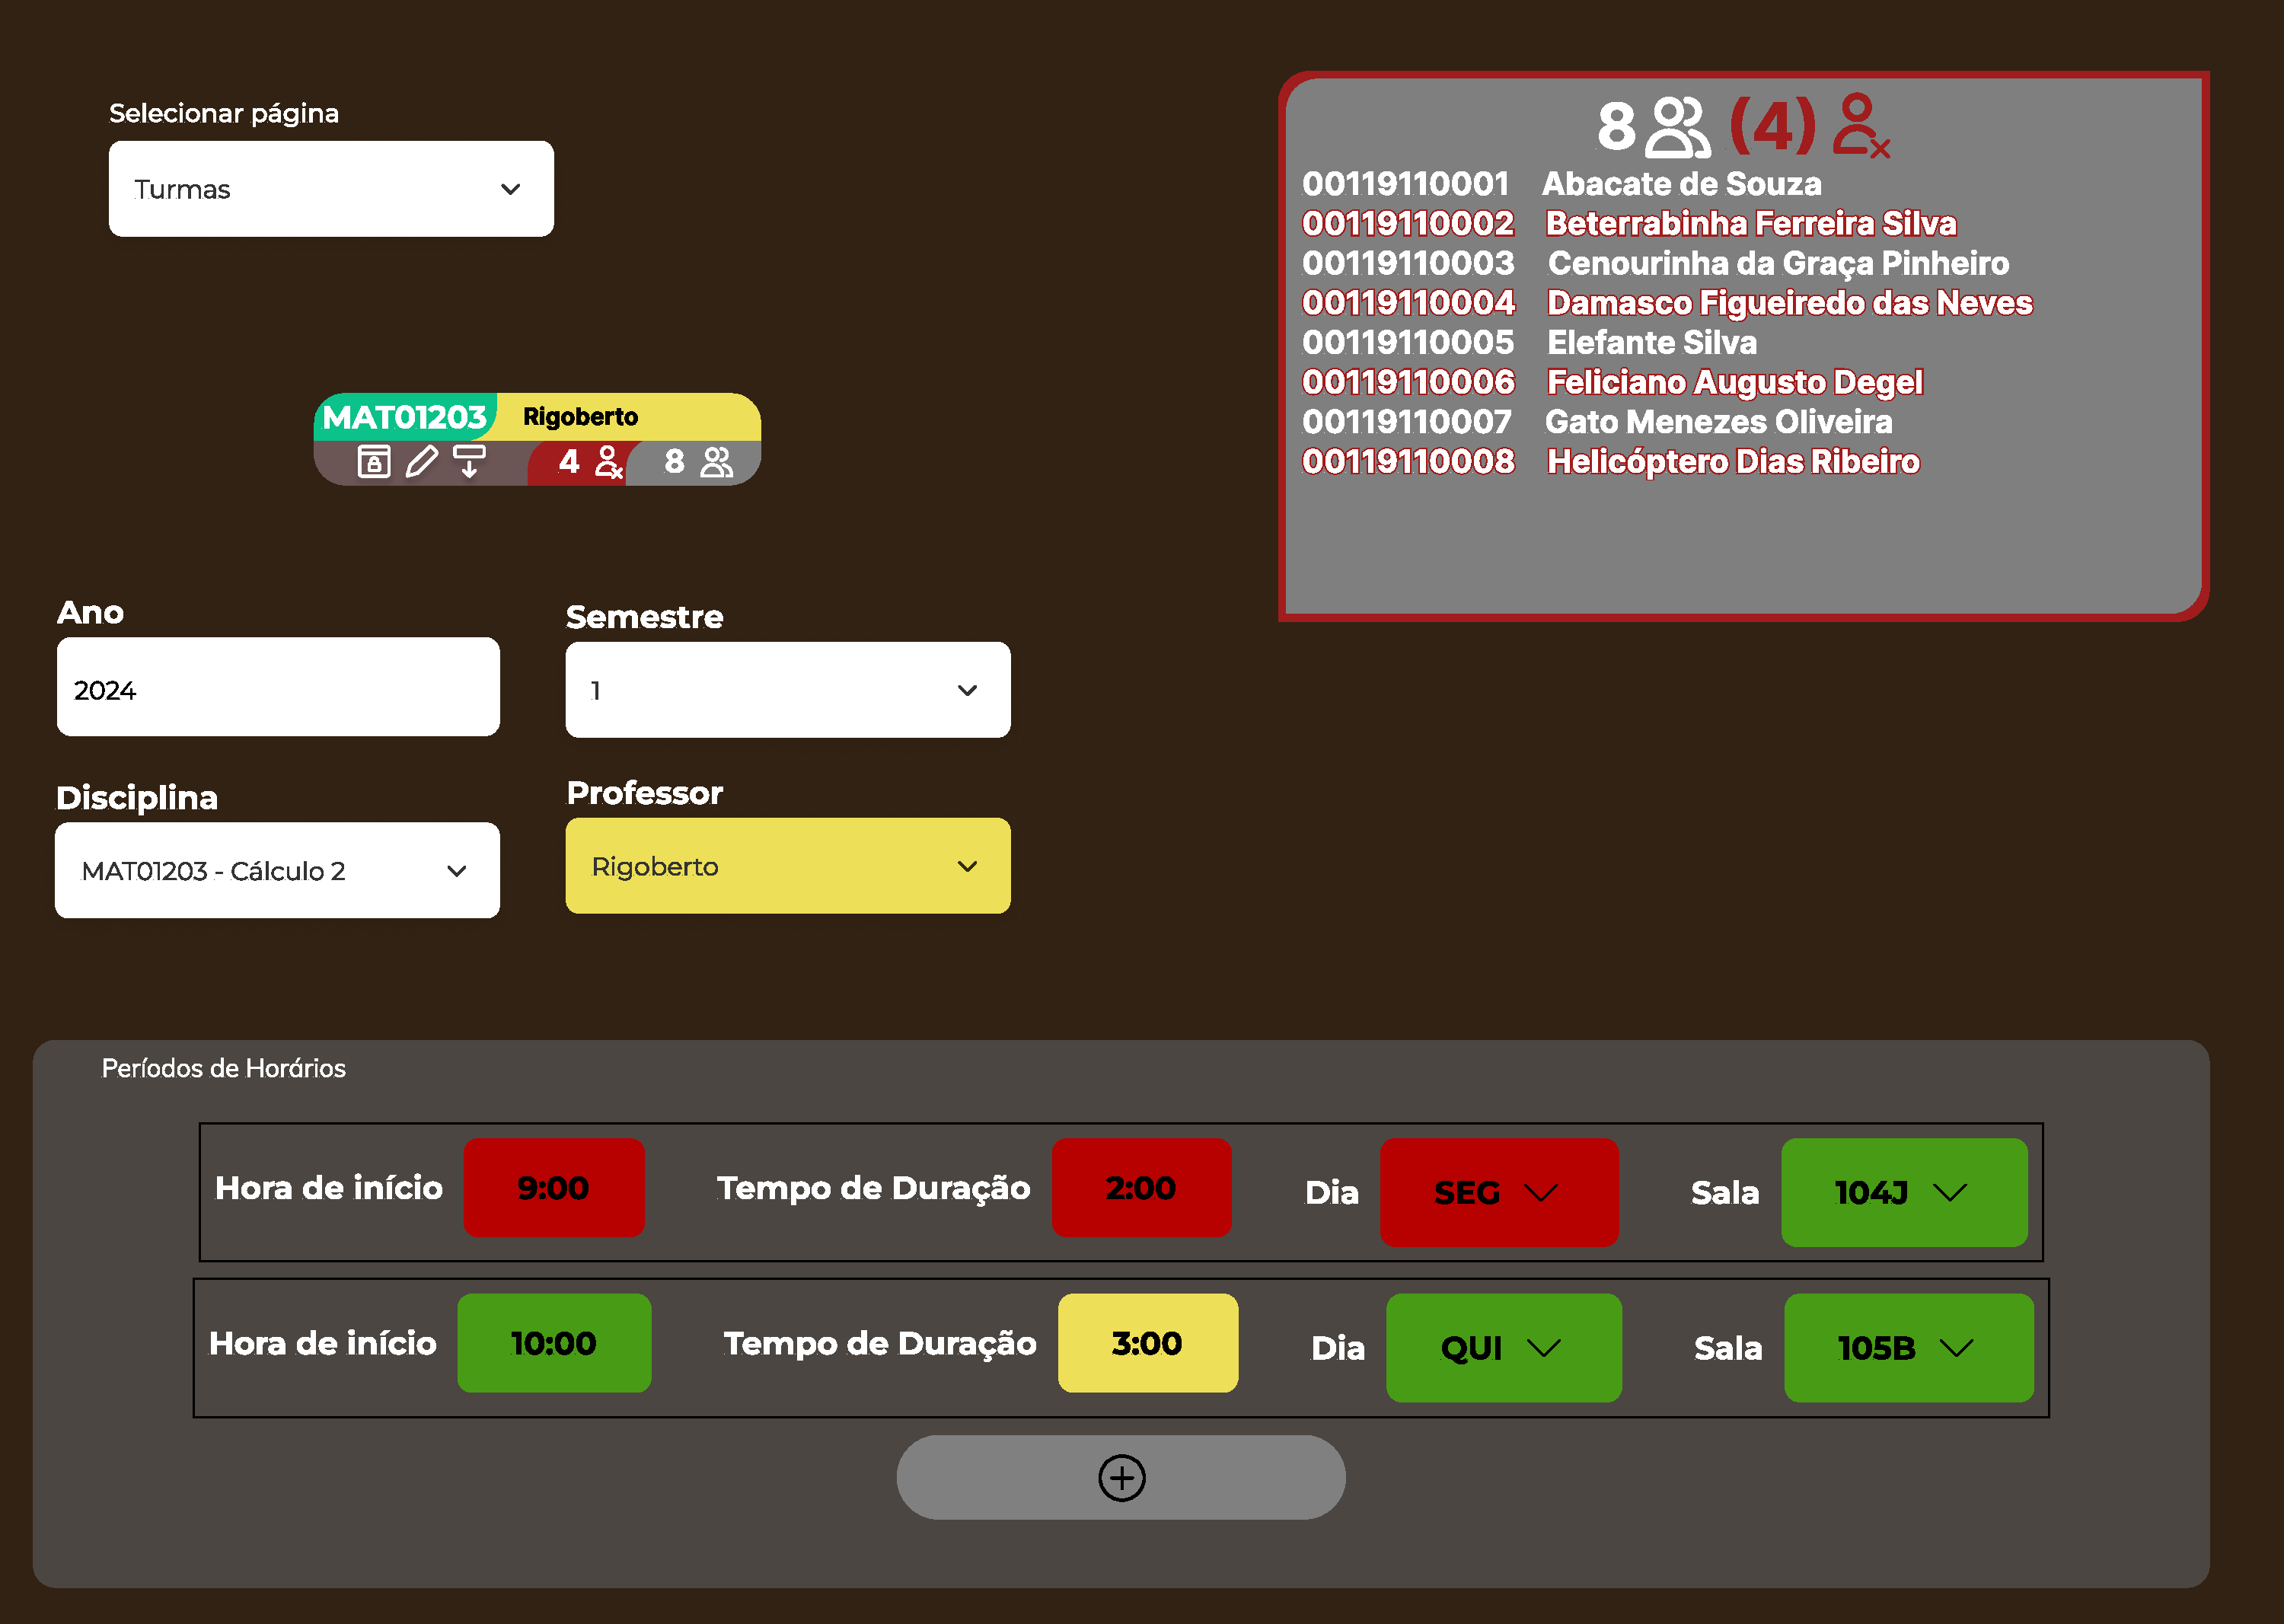
\includegraphics[width=\textwidth]{files/img/2.02!5-desenvolvimento/2.02!5.3-prototipagem/5.3.2-paginas/7-CRUD_turmas}
\end{MyCenteredFigure}

Ainda na \autoref{fig:CRUD_turmas} temos alguns exemplos de conflitos percebidos. O primeiro, com a cor amarelada, informado que o tempo de duração do segundo horário da turma não condiz com a preferência pessoal do professor selecionado. Este conflito não é impeditivo, entretanto, se possível, um outro horário poderia ser encontrado para atender melhor às preferências do professor.

Outro conflito exibido é que a sala em que está alocado o primeiro horário da turma já está ocupada no mesmo horário por outra turma. Este conflito é impeditivo, sendo então representado na cor vermelha. Neste caso, a turma deve ser realocada para outro horário ou sala.

Por último, na listagem dos alunos que podem se inscrever, no canto inferior direito, há quatro alunos marcados em vermelho. Estes alunos poderiam se inscrever em outra turma no mesmo horário em que esta turma está alocada. Este conflito é impeditivo, mas apenas para os alunos, assim como no caso da preferência do professor, a turma pode ser realocada para outro horário para atender melhor às demandas dos alunos.

\section{Programação do sistema} \label{sec:programação}                                % ###  5.4

Após a \hyperref[sec:ModelagemBD]{conceitualização diagramática do banco de dados} e a \hyperref[ssec:componentes]{elaboração dos protótipos com o Figma}, o desenvolvimento do sistema foi iniciado. Por maior familiaridade com a linguagem foi escolhida a linguagem \textbf{\textit{JavaScript}}, utilizando a biblioteca \textbf{\textit{React}} para a criação dos componentes visuais, ou seja, o \textit{frontend}, e o \textbf{\textit{Node.js}} para a criação do \textit{backend} e a criação de um servidor local que permite visualizar as mudanças no código em tempo real. Suas logos estão ilustrados na \autoref{fig:sistemas}.

\begin{MyCenteredFigure} \caption{Recursos usados para o desenvolvimento do sistema} \label{fig:sistemas}
  \begin{animateinline}[loop, autoplay]{1}
    \myAnimation{JavaScript} % 1 JS
    \myAnimation{React}      % 2 React
    \myAnimation{NodeJS}     % 3 Node
    \newframe
    \myAnimation{React}      % 2 React
    \myAnimation{NodeJS}     % 3 Node
    \myAnimation{JavaScript} % 1 JS
    \newframe
    \myAnimation{NodeJS}     % 3 Node
    \myAnimation{JavaScript} % 1 JS
    \myAnimation{React}      % 2 React
  \end{animateinline}
\end{MyCenteredFigure}

% Tang achou esse parágrafo confuso.
Seguindo constantemente o conceito de iteratividade da apresentação do sistema, a programação foi marcada por dois conceitos: blocos de funcionalidades marcantes e blocos de funcionalidades apresentadas. O primeiro conceito se refere à grandes grupos de mudanças que estavam relacionadas a um mesmo tópico, ou que resultaram, quando em conjunto, num sistema consideravelmente distinto de como estava antes de as receber. O segundo conceito se refere à apresentação esporádica da situação atual do sistema para quem o iria utilizar, sendo essas versões chamadas de MVPs (Minimum Viable Product - Mínimo Produto Viável).

Nesta seção serão apresentadas as versões do sistema repartidas de forma a apresentar os agrupamentos de mudanças notórias. Sua \hyperref[sec:programação]{programação} foi repartida em três grandes categorias que visavam entregar o sistema de forma gradual e funcional. A \hyperref[ssec:MVP1]{primeira versão do sistema} foi desenvolvida localmente com o objetivo de se aproximar ao máximo das páginas previstas no protótipo, sem a necessidade de um banco de dados que permitisse alterações. A \hyperref[ssec:MVP2]{segunda versão do sistema} contou com a utilização de duas abordagens distintas de bancos de dados para se obter a permanência dos dados. Já a \hyperref[ssec:MVP3]{terceira versão do sistema} foi desenvolvida de forma a estar completamente hospedada na nuvem, incluindo o seu banco de dados, sendo então \hyperref[sec:preenchimento]{preenchido com mais dados}.

\begin{MyCenteredFigure} \caption{Diagrama da progressão funcionamento da permanência dos dados} \label{fig:API}
  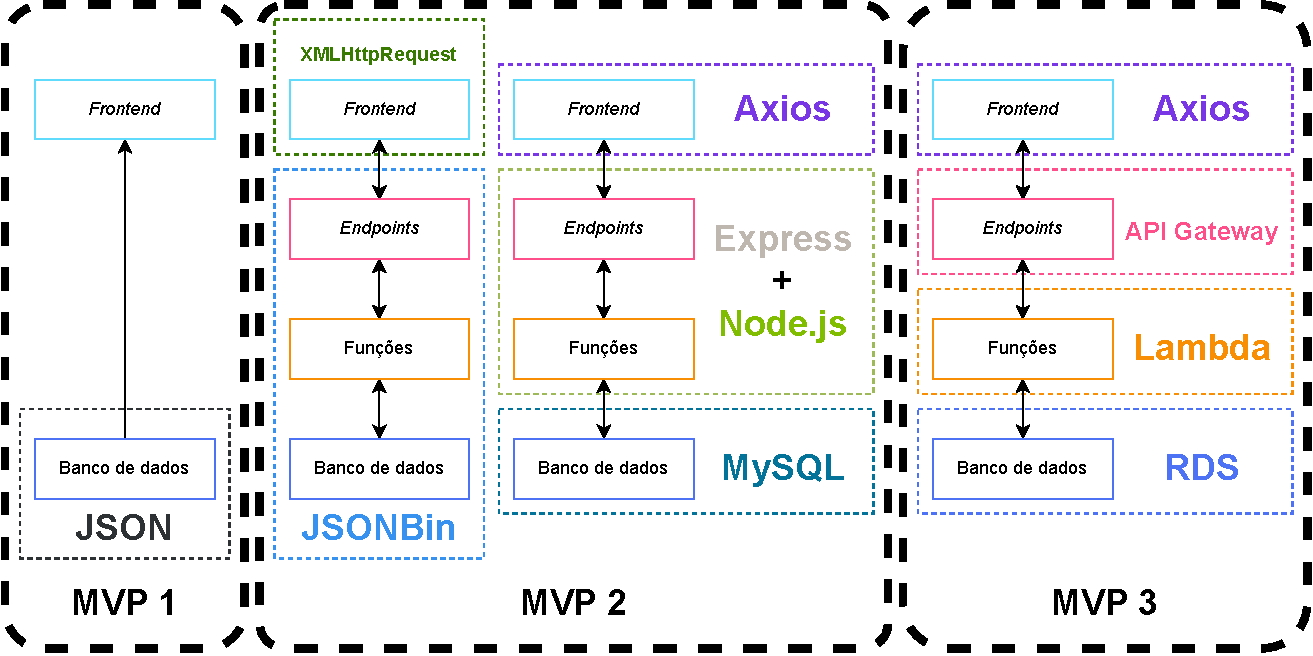
\includegraphics[width=\textwidth]{files/img/2.02!5-desenvolvimento/2.02!5.4-sistema/5.4.0-programacao/API-Progressão}
\end{MyCenteredFigure}

Ao longo da implementação dessas versões, diversos métodos de manutenção dos dados foram utilizados, como a importação de arquivos JSON, a utilização de um banco de dados local e a utilização de um banco de dados hospedado na nuvem. A \autoref{fig:API} ilustra a progressão do funcionamento da permanência dos dados ao longo das três versões do sistema. Os pormenores de cada versão serão descritos adiante.

\subsection{Versão 1.0} \label{ssec:MVP1}                                               % #### 5.4.1

A primeira versão do sistema foi desenvolvida inicialmente em um ambiente local, com o objetivo de se aproximar ao máximo das páginas previstas no protótipo. Para isso, foi utilizada a biblioteca \LinkToURL{\LinkReactRouter}{\textit{React Router}} para a navegação entre as páginas, e a biblioteca \LinkToURL{\LinkReactSelect}{\textit{React Select}} para as caixas de seleção. Ao final desta versão, o sistema foi hospedado no \hyperref[sssec:GitHub Pages]{GitHub Pages} no link \url{\LinkOurClass}.

\subsubsection*{\textbf{Banco de dados preliminar}} \label{sssec:BDInicial}

Os dados contidos no sistema foram inicialmente armazenados em arquivos JSON, que eram importados diretamente para o código (\autoref{fig:API_MVP1}). Isso foi feito para que fosse possível visualizar o funcionamento do sistema sem a necessidade de um banco de dados real. A partir disso, foi possível visualizar o funcionamento do sistema e realizar testes de usabilidade. Em contrapartida, os dados disponíveis não eram modificáveis, tendo apenas a possibilidade de leitura e mutação temporária, visto que após recarregar ou mudar de página, as mudanças eram perdidas.

\begin{MyCenteredFigure} \caption{Diagrama do armazenamento preliminar dos dados} \label{fig:API_MVP1}
  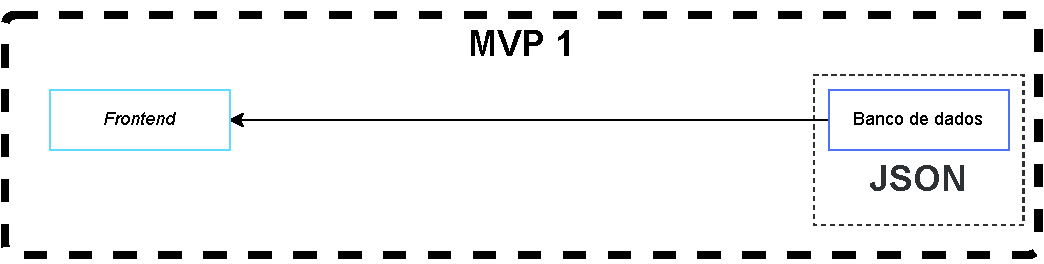
\includegraphics[width=\textwidth]{files/img/2.02!5-desenvolvimento/2.02!5.4-sistema/5.4.1-MVP1/API_MVP1}
\end{MyCenteredFigure}

Nesse método, cada entidade era armazenada em um arquivo JSON separado, contendo esse um array de objetos, onde em cada objeto haviam as chaves, representando as propriedades da entidade, e os valores, representando os dados da entidade.

Como nesta dinâmica não havia uma forte correlação entre os dados, o \textit{frontend} acabava sendo o responsável por unir todas as informações. Assim, por exemplo, para se obter a lista de professores de uma turma, era necessário importar todos os professores, todas as turmas, e então, a partir do nome do professor alocado àquela turma, buscar na listagem dos professores qual era o professor que correspondia àquele nome, para então agregar as informações.

\subsubsection*{\textbf{Funcionalidades iniciais: CRUD e primeiros conflitos}} \label{sssec:Funcionalidades Iniciais}

Nessa primeira versão, algumas funcionalidades já começaram a ser esboçadas, principalmente as funcionalidades CRUD (\textit{Create}, \textit{Read}, \textit{Update}, \textit{Delete}) para as entidades principais do sistema. Embora, como já dito, os dados não fossem persistentes, foi possível visualizar o funcionamento das funcionalidades de criação e leitura de turmas, professores, disciplinas, salas e horários.

Nessa versão, também foi implementada uma checagem bruta de conflitos por alocação simultânea de professores em mais de uma turma e a checagem da quantidade de demanda de alunos em relação à capacidade das salas. Uma descrição mais detalhada das funcionalidades de conflitos está presente adiante na \autoref{sec:conflitos} denominada \nameref{sec:conflitos}.

\subsubsection*{\textbf{Preferências dos professores, progressão dos alunos e recursos da sala}} \label{sssec:Progressão dos Alunos e Preferência dos Professores}

Além das funcionalidades citadas anteriormente que se mantiveram até a conclusão do sistema, também foram desenvolvidas funcionalidades que não obtiveram o mesmo êxito e que foram deixadas de lado. Dentre elas, podemos citar a definição de níveis de \textbf{preferência de horários para professores}, a \textbf{progressão dos alunos} em relação às disciplinas, e a definição das \textbf{características especiais das salas}.

A tabela de preferências de horários para professores foi desenvolvida e consistia em permitir a definição de níveis de preferência para cada um dos horários da semana. A ideia era que, ao alocar as turmas, o sistema pudesse priorizar os horários que fossem mais bem avaliados pelos professores, assim aumentando sua satisfação sempre que possível. A funcionalidade foi descartada por ser considerada de menor prioridade em relação a outras funcionalidades, segundo a coordenação de computação, não sendo ela um dos fatores mais relevantes para a definição das grades horárias no curso de Ciência da Computação.

\subsubsection*{\textbf{GitHub Pages}} \label{sssec:GitHub Pages}

Após o desenvolvimento local foi feita a implementação da interface do sistema para um servidor online. Para isso, foi utilizado o serviço \LinkToURL{\LinkGitHubPages}{GitHub Pages} que, por ser gratuito e de fácil utilização, foi a escolha mais adequada para o momento.

Para implantar no GitHub Pages o código desenvolvido, utilizou-se da \LinkToURL{\LinkBibliotecaGHPages}{biblioteca gh-pages}, que viabiliza a publicação de um site diretamente do repositório do GitHub. A partir disso, o sistema foi disponibilizado para acesso público, permitindo que qualquer pessoa pudesse acessar o sistema e testar suas funcionalidades no endereço eletrônico \url{\LinkOurClass}.

\subsection{Versão 2.0} \label{ssec:MVP2}                                               % #### 5.4.2

Utilizando do \textit{feedback} quanto aos resultados entregues na \hyperref[ssec:MVP1]{primeira versão}, alguns pontos de melhoria foram identificados, sendo um deles, e o mais importante: o planejamento. Na primeira abordagem, o desenvolvimento foi feito seguindo notas e ideias soltas, sem um planejamento prévio, o que resultou em um sistema que, embora funcional, não atendia a todas as necessidades propostas. Também dispunha de funcionalidades que não eram de todo necessárias, ou, melhor dizendo, que tinham menor prioridade do que muitas outras. Como solução, foi utilizado o \hyperref[sssec:GitHub Projects]{GitHub Projects} para organizar as tarefas e priorizá-las.

% Mesmo com esta nova dinâmica, outras funcionalidades foram deixadas de lado. Uma das que foram deixadas de lado foi a possibilidade de fixar certas informações. A proposta era que, certas disciplinas que são ofertadas para múltiplos cursos, pudessem ser fixadas em horários específicos, para que simplificasse aos criadores de grades horárias a alocação de turmas.

% Nessa versão, também foram utilizados dois métodos de manutenção dos dados o \hyperref[ssssec:JSONBin]{JSONBin} que não atingiu às expectativas e o \hyperref[ssssec:MySQL]{MySQL} que serviu para a criação de um banco de dados local, já emulando o \hyperref[sssec:Amazon Web Services]{posterior uso de um banco de dados hospedado na nuvem}.

Seguindo o planejamento feito, uma das primeiras tarefas foi a implementação do banco de dados que permitisse a \hyperref[sssec:Permanência dos Dados]{permanência dos dados}, para isso, foram utilizados dois métodos de manutenção dos dados: o \hyperref[ssssec:JSONBin]{JSONBin} e o \hyperref[ssssec:MySQL]{MySQL}. Outro ponto foi a criação da \hyperref[sssec:Logomarca]{logomarca} do sistema, que foi feita para que o sistema tivesse uma identidade visual própria. Foram desenvolvidas também \hyperref[sssec:Funcionalidades Adicionais]{algumas outras funcionalidades}, como a análise de conflitos adicionais, a possibilidade de se filtrar as turmas e a visualização de disciplinas que ainda não têm uma turma criada no semestre em planejamento.

\subsubsection*{\textbf{GitHub Projects}} \label{sssec:GitHub Projects}

Utilizando o \LinkToURL{\LinkGitHubProjects}{GitHub Projects}, foi organizada uma tabela de tarefas, vista na \autoref{fig:GitHubProjectsTable}, onde foram unificadas as diversas anotações e ideias, antes soltas. A partir disso, foi possível visualizar o que era mais importante e o que poderia ser deixado de lado.

\begin{MyCenteredFigure} \caption{Tabela de tarefas do GitHub Projects} \label{fig:GitHubProjectsTable}
  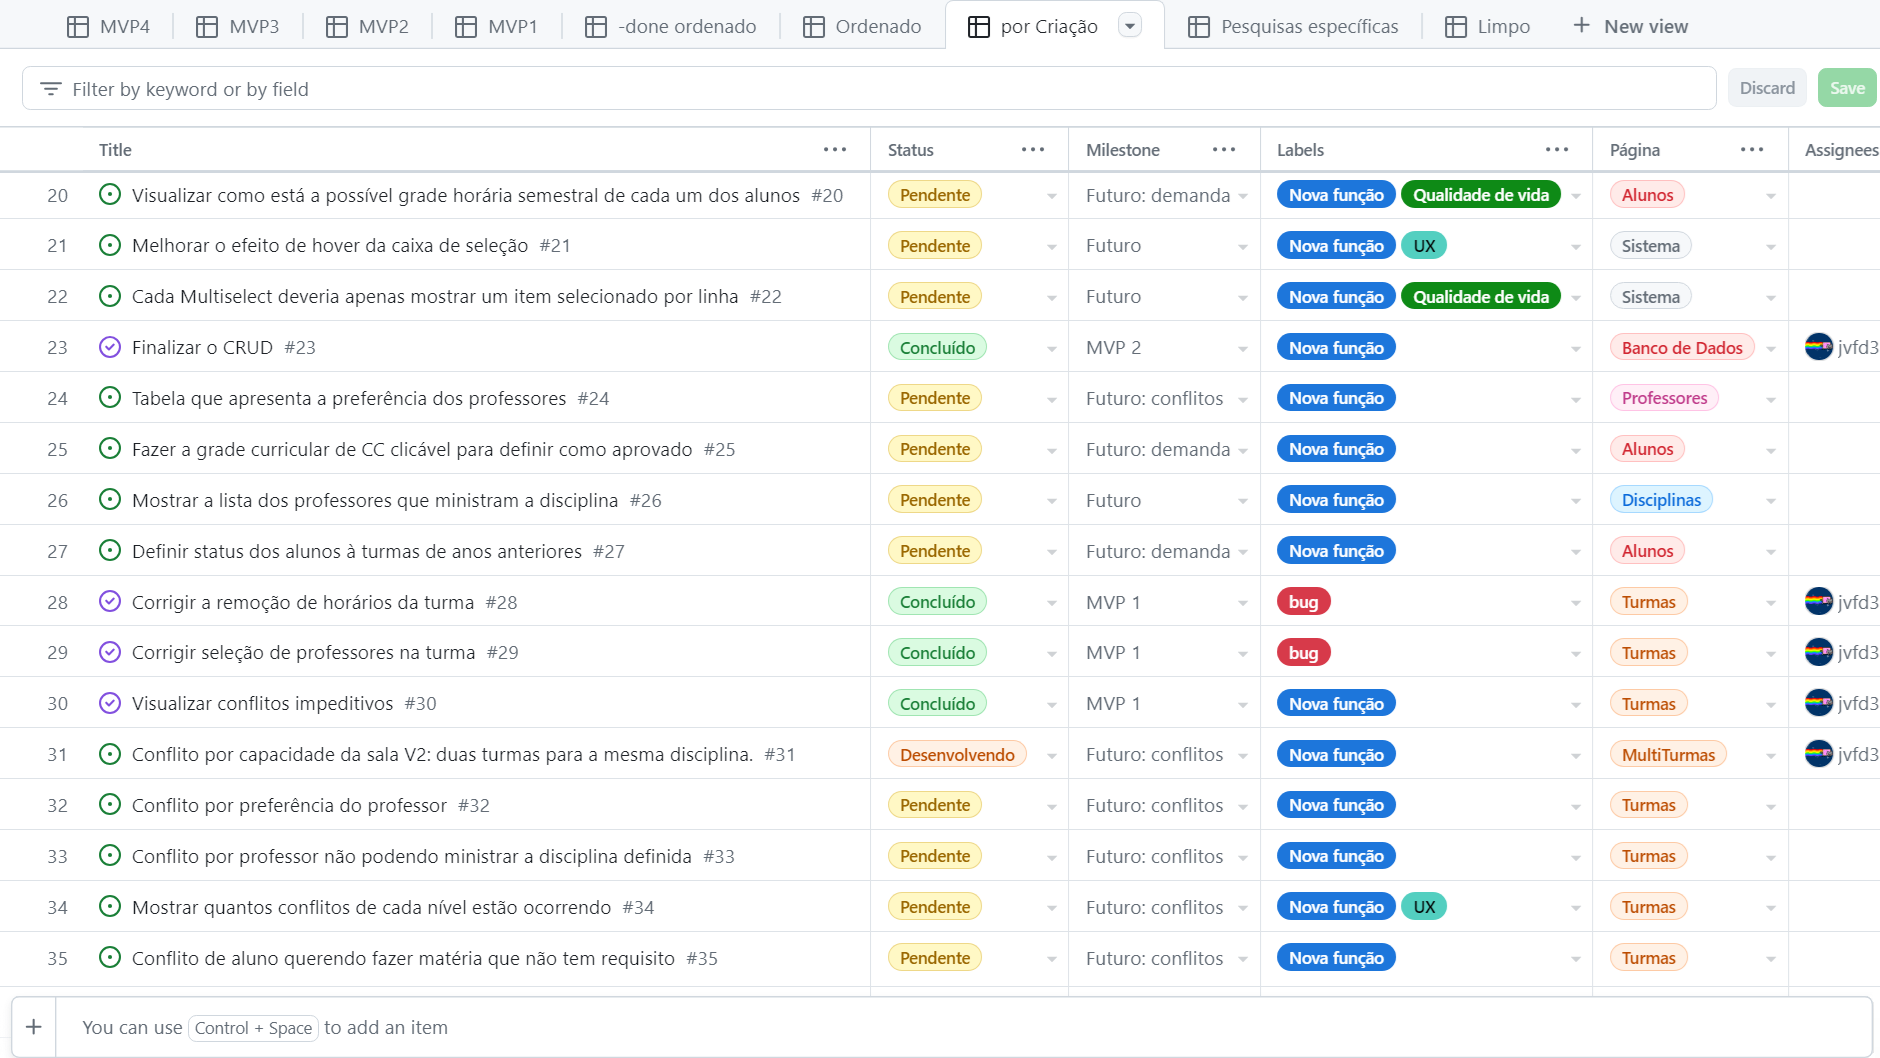
\includegraphics[width=\textwidth]{files/img/2.02!5-desenvolvimento/2.02!5.4-sistema/5.4.2-MVP2/GitHubProjects-Table-Light}
\end{MyCenteredFigure}

Tendo este novo sistema de tarefas em prática, foi possível planejar melhor quais eram as funcionalidades que precisavam ser desenvolvidas, as que já estavam prontas, as que poderiam ter melhorias e quais se desejava implementar no futuro.

As tarefas foram inicialmente divididas em três principais categorias: \textit{Status}, \textit{Página} e \textit{Sequência}. O \textit{Status} reflete o andamento do código da tarefa, podendo ser este andamento \textbf{Pendente}, \textbf{Desenvolvendo}, ou \textbf{Concluído}. A \textit{Página} reflete em qual página do sistema a tarefa se encontra, e a \textit{Sequência} reflete a ordem de prioridade da tarefa.

Citando mais detalhes da \autoref{fig:GitHubProjectsTable}, temos à esquerda a numeração das tarefas, seguido do título da tarefa que descreve em poucas palavras sobre o que se trata. ao final do título há uma combinação do símbolo ``\#'' e uma numeração. Essa numeração representa a sequência de criação das tarefas, código esse que pode ser usado como referência entre as tarefas, assim permitindo que tarefas correlacionadas tenham um link direto entre elas. Na próxima coluna está o \textit{Status} da tarefa, seguido de duas colunas, \textbf{\textit{Milestone}} e \textbf{\textit{Labels}} que só foram criadas \hyperref[ssssec:Marcos e Etiquetas]{posteriormente}. Finalizando temos a coluna \textbf{Página} que primariamente distingue em qual página do sistema a tarefa se encontra, mas que também contém algumas categorias que fogem do conceito de página, como por exemplo é o caso das categorias ``Componente'', ``Sistema'' e ``Banco de Dados''. Por último há a coluna \textit{Assignees} que indica quem é o responsável pela tarefa; nesse caso, todas as tarefas que estão em andamento ou que já se encontram concluídas foram atribuídas ao mesmo responsável.

\subsubsection*{\textbf{Permanência na alteração dos dados}} \label{sssec:Permanência dos Dados}

Tendo agora uma rota mais clara a ser seguida, o desenvolvimento foi retomado. Uma das características mais marcantes e ainda não atribuídas ao sistema era a manutenção das modificações feitas nos dados. Nesta etapa, foram utilizados dois métodos de se manter as alterações feitas aos dados. Com esse intuito foram utilizados dois métodos de manutenção dos dados o \hyperref[ssssec:JSONBin]{JSONBin} que não atingiu às expectativas e o \hyperref[ssssec:MySQL]{MySQL} que serviu para a criação de um banco de dados local, já emulando o posterior uso de um \hyperref[sssec:Amazon Web Services]{banco de dados hospedado na nuvem}. Como nessa etapa houveram esses dois métodos de manutenção dos dados, a \autoref{fig:API_MVP2} ilustra o paralelo entre os dois métodos.

\begin{MyCenteredFigure} \caption{Comparação entre bancos de dados da Versão 2.0} \label{fig:API_MVP2}
  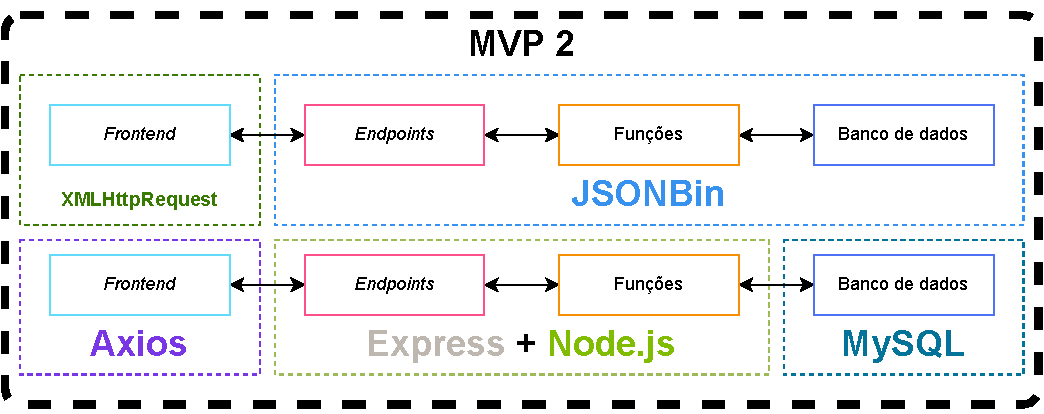
\includegraphics[width=\textwidth]{files/img/2.02!5-desenvolvimento/2.02!5.4-sistema/5.4.2-MVP2/API_MVP2}
\end{MyCenteredFigure}

\subsubsubsection*{A) \LinkToURL{\LinkJSONBin}{JSONBin}} \label{ssssec:JSONBin}

Como até então os dados estavam armazenados em formato JSON, imaginou-se que a melhor forma de persistir os dados seria através de um banco de dados que lidasse com JSON, o escolhido para este fim foi o JSONBin por apresentar ser uma plataforma gratuita e de fácil utilização.

Esta plataforma permite a criação de \textit{bins}, que são basicamente coleções de dados em formato JSON. A partir disso, é possível realizar requisições HTTP para a leitura, escrita, atualização e remoção dos dados. A utilização do JSONBin foi feita através de requisições HTTP usando o objeto \textit{XMLHttpRequest} do JavaScript, e a comunicação entre o \textit{frontend} e o JSONBin foi feita através de \textit{tokens} de acesso. Este fluxo é representado pela seção superior da \autoref{fig:API_MVP2}.

Com isso, se tornou possível ler e atualizar os dados de forma remota, e assim, manter os dados mesmo após a recarga da página. Embora cumprisse com o que promete e o que era desejado, o JSONBin não se mostrou a melhor escolha para o sistema, visto que a sua utilização não performou tão bem quanto se esperava.
% Não se sabe se foi por inexperiência ou por limitações do próprio serviço, mas
A utilização do JSONBin para a coleta dos dados, fazia com que a tela de carregamento do sistema demorasse alguns segundos para ser exibida, o que não é apropriado para a usabilidade do sistema proposto.

\subsubsubsection*{B) \LinkToURL{\LinkMySQL}{MySQL}} \label{ssssec:MySQL}

Embora houvesse o desejo do uso de informações em formato JSON, achou-se por bem utilizar um banco de dados mais usual, recorrendo então ao MySQL, sendo então necessário criar um banco de dados local que armazenasse os dados e que pudesse ser acessado pelo sistema. Essa configuração serviu para estabelecer a supracitada camada de banco de dados. E consistiu basicamente na instalação do MySQL Server.

\paragraph*{B1) Migração dos dados}

Como os dados se encontravam em formato JSON, primariamente utilizou-se da ferramenta de importação de dados do próprio \textbf{MySQL Workbench}. Durante essa importação, o software automaticamente identifica os campos, criando a tabela e suas colunas. Porém, devido à quantidade dos dados, essa importação tendia a ser demorada, e por vezes, falhava
% , sem haver uma explicação clara do porquê
.

Com isso, foi necessário recorrer a uma abordagem semimanual, sendo então desenvolvido um código em Python que lê os arquivos JSON e os converte em arquivos SQL para que as \textit{queries} pudessem ser executadas no MySQL Workbench. A partir disso, foi possível importar os dados de forma mais rápida e eficiente.

Apesar da primeira tentativa de importação não ter sido completamente bem sucedida, foi desta forma que as tabelas, representadas pela \autoref{fig:TabelasIniciais}, foram inicialmente criadas. Isso gerou posteriormente a necessidade de ajustes manuais, como a adição de chaves primárias e estrangeiras, e a alteração de tipos de dados. Porém, como neste momento, o sistema visava apenas replicar o funcionamento do JSONBin, essas alterações não foram feitas de imediato.

\begin{MyCenteredFigure} \caption{Diagrama inicial das tabelas de dados SQL} \label{fig:TabelasIniciais}
  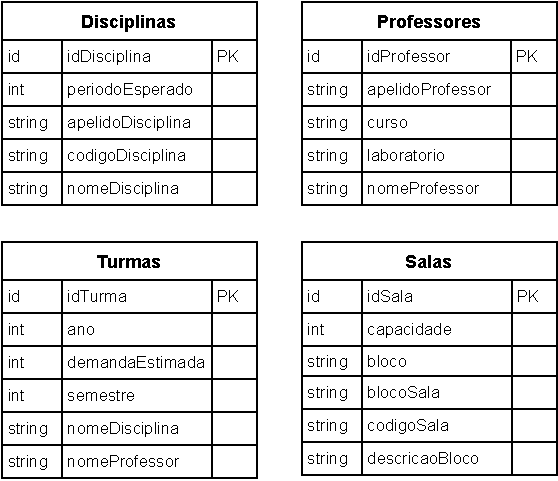
\includegraphics[width=0.7\textwidth]{files/img/2.02!5-desenvolvimento/2.02!5.4-sistema/5.4.2-MVP2/Diagrama_ER-As_is}
\end{MyCenteredFigure}

\paragraph*{B2) Acesso ao Banco de Dados}

Seguindo a mesma sequência de camadas, o acesso ao banco de dados continua sendo feito através de requisições HTTP, porém, ao invés de serem enviadas ao JSONBin, são enviadas a um servidor local que executa as operações no banco de dados. Essa modificação é representada pela seção inferior da \autoref{fig:API_MVP2}.

No \textit{frontend}, enquanto que para acessar a API já pronta do JSONBin foi utilizado o objeto \textit{XMLHttpRequest}, para a comunicação com o banco de dados local, foi utilizada a biblioteca \LinkToURL{\LinkAxios}{\textit{Axios}} para construir as requisições HTTP. E elas, ao invés de serem enviadas ao JSONBin, são enviadas ao \textbf{servidor local}.

Na criação deste \textbf{servidor local} utilizou-se a biblioteca \LinkToURL{\LinkExpress}{\textit{Express}} para desenvolver um \textit{backend} local executado com o \LinkToURL{\LinkNodeJS}{Node.js} paralelo ao \textit{frontend}. Essa biblioteca é responsável por criar todas as rotas necessárias para a comunicação entre o \textit{frontend} e o banco de dados. A partir disso, foi possível criar rotas para cada uma das entidades, e para cada uma das operações CRUD. Com isso, cada operação CRUD em cada uma das rotas é encaminhada para uma \textbf{função específica} que executa a operação no banco de dados.

Este uso, embora exemplifique a aplicação da permanência dos dados, está limitado por dois aspectos: em primeira instância, a permanência dos dados é limitada ao servidor local, não sendo este o desejo final do sistema. Em segunda instância, para haver o acesso aos dados, é necessário que, além do banco de dados, o \textit{backend} também esteja em execução, entretanto, o GitHub Pages, onde o sistema está hospedado, não viabiliza essa execução. Com isso viu-se necessária a busca por um serviço de hospedagem que disponibilizasse a execução do \textit{backend}.

\subsubsection*{\textbf{Logomarca}} \label{sssec:Logomarca}

Um dia após o Natal, foi criado um dos arquivo do sistema chamado ``hourclassMagic.js'', este arquivo agrupava funções que consistiam basicamente em adicionar e remover horários (\textit{hour}) e turmas (\textit{class}) da listagem de turmas e horários. Porém, considerando que a junção dos nomes \textit{hour} e \textit{class} era consideravelmente similar à palavra \textit{hourglass} (``ampulheta'' em inglês) e que a ampulheta é um símbolo que remete ao tempo, e que o sistema é um sistema de alocação de horários, optou-se por utilizar a ampulheta como símbolo do sistema. Quanto ao nome, como o sistema visa a alocação de turmas, especificamente para o curso de Ciência da Computação na UENF, decidiu-se pela corruptela da palavra \textit{hour} para que se tornasse \textit{our}, que significa ``nosso'' em inglês, assim, remetendo ao sentido de individualidade do sistema. Com isso, o nome do sistema se tornou \textit{OurClass}.

\begin{MyCenteredFigure} \caption{Logomarcas do sistema} \label{fig:Logomarcas}
  
\includegraphics[width=\textwidth]{files/img/2.02!5-desenvolvimento/2.02!5.4-sistema/5.4.2-MVP2/Logomarcas}
\end{MyCenteredFigure}

Juntando o símbolo da ampulheta com o nome \textit{OurClass} e outros elementos gráficos, como as tabelas horárias, foi criada a logomarca do sistema, que pode ser vista na \autoref{fig:Logomarcas}. A logomarca foi criada utilizando de inteligências artificiais generativas, principalmente o \textit{Bing}. A partir disso, foi possível criar uma logomarca que refletisse o propósito do sistema, e que fosse agradável visualmente. Após analisar as possibilidades, foi escolhida a \autoref{fig:logomarca_oficial} como a logomarca oficial do sistema. A logomarca foi então adicionada ao sistema.

\begin{MyCenteredFigure} \caption{Logomarca oficial} \label{fig:logomarca_oficial}
  
\includegraphics[width=0.5\textwidth]{files/img/2.02!5-desenvolvimento/2.02!5.4-sistema/5.4.2-MVP2/OurClass}
\end{MyCenteredFigure}

\subsubsection*{\textbf{Funcionalidades adicionais: conflitos, filtragem e disciplinas não oferecidas}} \label{sssec:Funcionalidades Adicionais}

Acrescendo à visualização de conflitos desenvolvida na primeira versão, foi implementada a visualização de conflito por capacidade de salas, ao comparar com a quantidade de alunos estimados para a turma. Mais detalhes sobre os conflitos podem ser vistos mais adiante na \autoref{sec:conflitos} denominada \nameref{sec:conflitos}.

Adicionou-se também diversas filtragens, principalmente na página de \textbf{Grade Horária}. Dessa forma, torna-se possível a visualização específica de turmas que atendam a certos critérios. Essa filtragem é feita através de caixas de seleção, onde é possível selecionar quais critérios se deseja filtrar, sendo eles: ano, semestre, disciplina, professor, sala e categoria. Nessa última distinguem-se as disciplinas por períodos esperados para uma disciplina do curso de Ciência da Computação, e até mesmo, se são opcionais ou de outros cursos. Essa coletânea de filtros viabiliza uma análise mais limpa das informações estruturadas, podendo então gerar \textit{insights} quanto ao posicionamento histórico das turmas.

Outra utilidade adicionada, agora na página \textbf{MultiTurmas}, foi a seção de ``Disciplinas ainda não oferecidas''. Sua funcionalidade consiste em dispor ao usuário uma lista de disciplinas que, segundo a matriz curricular de Ciência da Computação, deveriam ser ofertadas naquele semestre. A partir disso, o usuário pode então selecionar o botão correspondente àquela disciplina e, a partir disso, uma turma para esta disciplina é adicionada à lista de turmas ofertadas. Há também um botão no topo que permite a adição de todas as disciplinas de uma vez.

\subsection{Versão 3.0} \label{ssec:MVP3}                                               % #### 5.4.3

A primeira versão trouxe a possibilidade de se visualizar o sistema, a segunda trouxe a possibilidade de se manter os dados. A terceira e última versão do sistema foi desenvolvida de forma a estar completamente hospedada na nuvem, incluindo o seu banco de dados. Assim como na versão anterior, alguns novos ajustes foram feitos na definição e distribuição de tarefas no \hyperref[sssec:GitHub Projects]{GitHub Projects}. Mas os dois principais focos desta versão foram o uso da \hyperref[sssec:Amazon Web Services]{Amazon Web Services} para a hospedagem do banco de dados e a \hyperref[sec:Solução inicial]{reimplementação da heurística para criação de uma grade horária inicial}.

\subsubsection*{\textbf{Mudanças no GitHub Projects}} \label{sssec:Mudanças no GitHub Projects}

O uso do GitHub Projects se provou como uma excelente forma de organização das tarefas, e assim, foi mantido para a terceira versão. Alguns novos detalhes foram adicionados em sua organização, como a adição da categorização de tarefas por \textbf{Marcos} (\textit{Milestones}) e \textbf{Etiquetas} (\textit{Labels}).

\begin{MyCenteredFigure} \caption{Marcos concluídos do GitHub Projects} \label{fig:ProjectsClosedMilestones}
  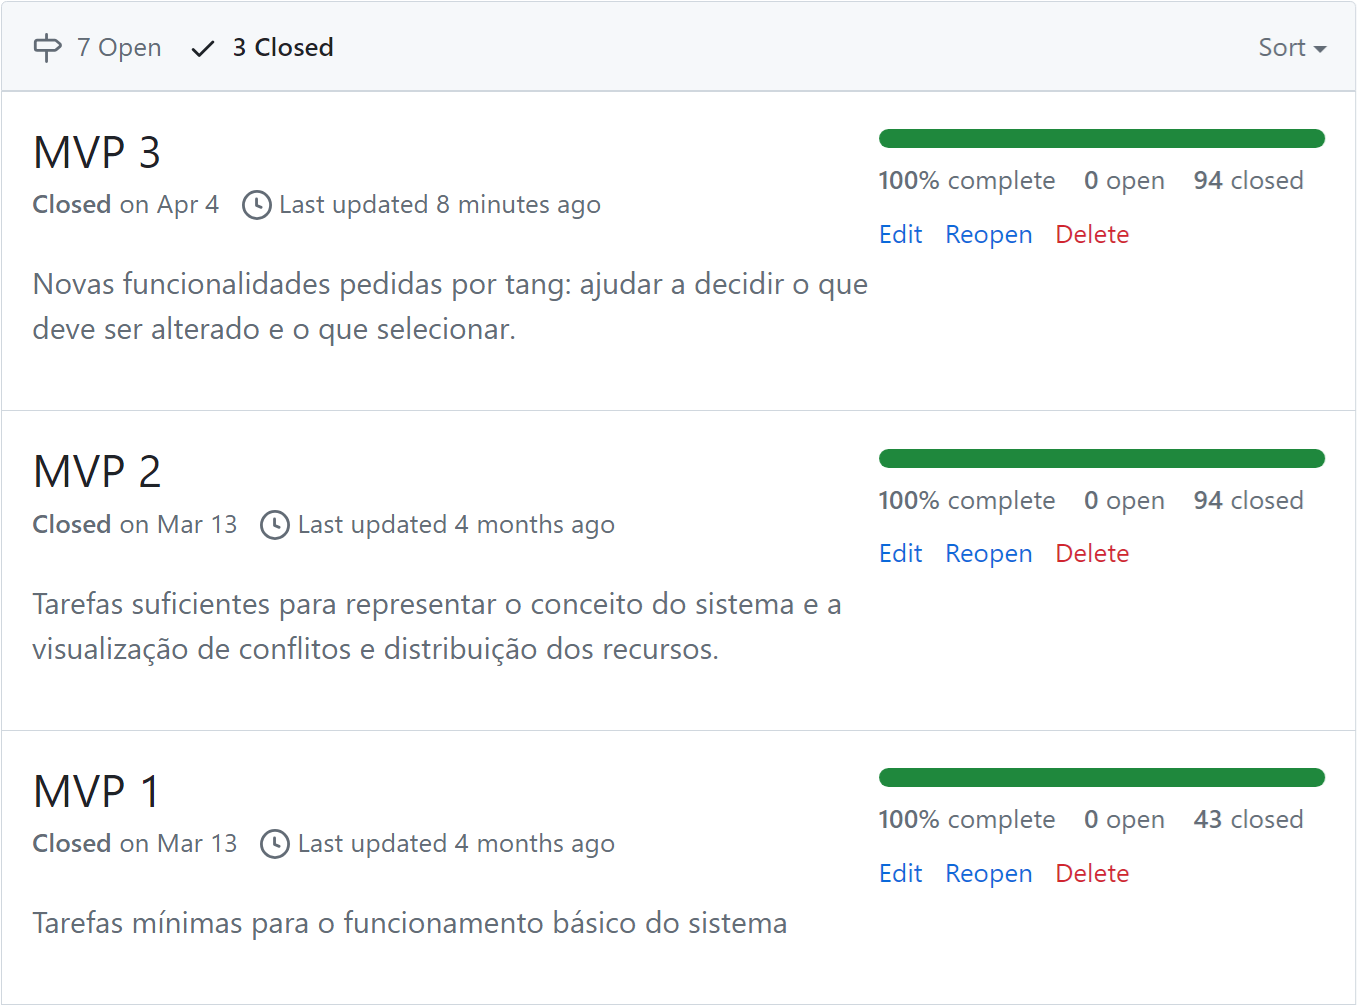
\includegraphics[width=0.9\textwidth]{files/img/2.02!5-desenvolvimento/2.02!5.4-sistema/5.4.3-MVP3/GitHubProjects-Closed_Milestones-Light}
\end{MyCenteredFigure}

\subsubsubsection*{A) Marcos e Etiquetas} \label{ssssec:Marcos e Etiquetas}

Os \textbf{Marcos} visam distinguir as tarefas por suas versões, e também por seus tipos de funcionalidades futuras, assim, a medida em que surgiam novas ideias, elas eram adicionadas ao GitHub Projects. Dessa forma, garantindo uma metrificação do andamento de cada categoria de funcionalidades, além de afunilar a quantidade de tarefas realmente prioritárias para o sistema.

\begin{MyCenteredFigure} \caption{Marcos abertos do GitHub Projects} \label{fig:ProjectsOpenMilestones}
  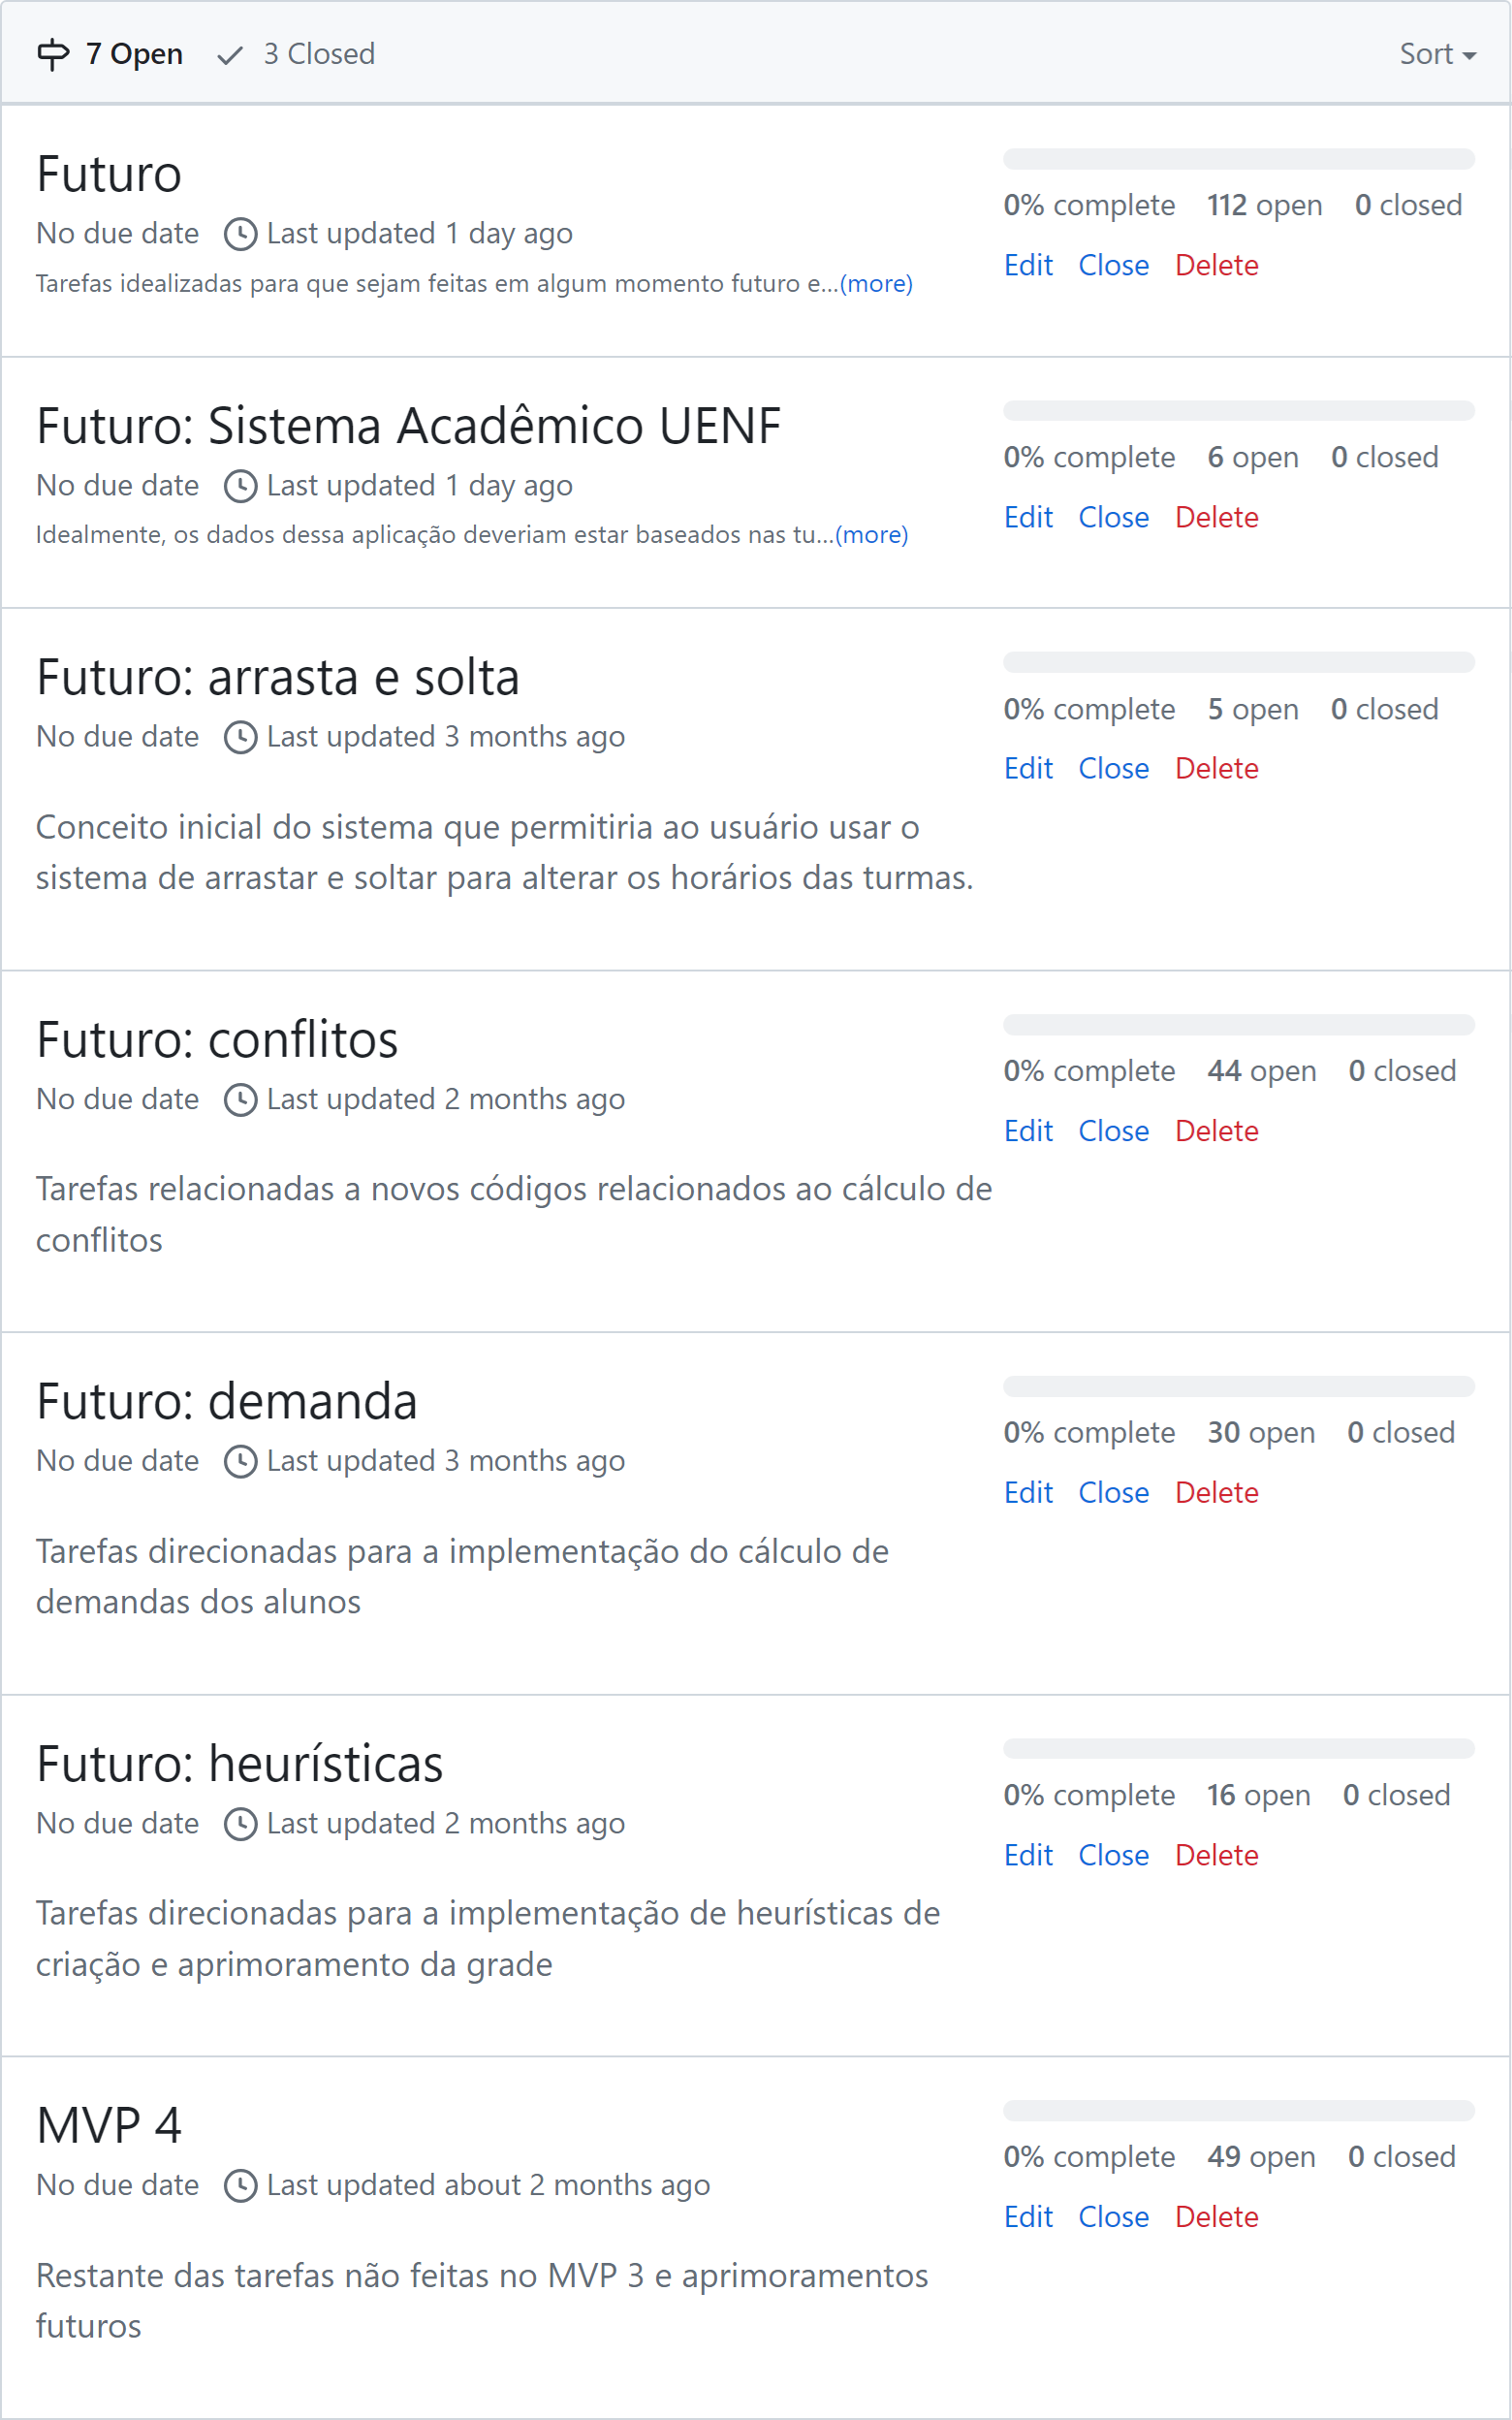
\includegraphics[width=0.9\textwidth]{files/img/2.02!5-desenvolvimento/2.02!5.4-sistema/5.4.3-MVP3/GitHubProjects-Open_Milestones-Light}
\end{MyCenteredFigure}

A \autoref{fig:ProjectsClosedMilestones} mostra os marcos que já foram concluídos, sendo eles as três versões desenvolvidas, e a \autoref{fig:ProjectsOpenMilestones} mostra os marcos que ainda estão em aberto, podendo ser retomadas no futuro.

\begin{itemize}
  \item Marcos Abertos
        \begin{enumerate}
          \item \textbf{MVP 1}: foram concluídas na primeira versão;
          \item \textbf{MVP 2}: foram concluídas na segunda versão;
          \item \textbf{MVP 3}: foram concluídas na terceira versão;
        \end{enumerate}
  \item Marcos Fechados
        \begin{enumerate}
          \item \textbf{MVP 4}: planejadas para a próxima versão a ser desenvolvida;
          \item \textbf{Futuro}: foram planejadas para o futuro do sistema;
          \item \textbf{Heurísticas}: visam aprimorar a alocação de turmas através de heurísticas;
          \item \textbf{Conflitos}: visam aprimorar a visualização, qualidade e/ou variedade de conflitos;
          \item \textbf{Integração com o Sistema Acadêmico UENF}: visam a integração do atual sistema com o sistema acadêmico da UENF.
          \item \textbf{Arrasta e solta}: visam aprimorar a alocação de turmas através de um sistema de arrastar e soltar;
          \item \textbf{Demandas}: visam calcular a demanda dos alunos por disciplinas;
        \end{enumerate}
\end{itemize}

No GitHub Projects, também foram adicionadas as \textbf{etiquetas} (\autoref{fig:ProjectsLabels}) que distinguem as tarefas por seu intuito. As etiquetas utilizadas foram as seguintes:

\begin{MyCenteredFigure} \caption{Etiquetas do GitHub Projects} \label{fig:ProjectsLabels}
  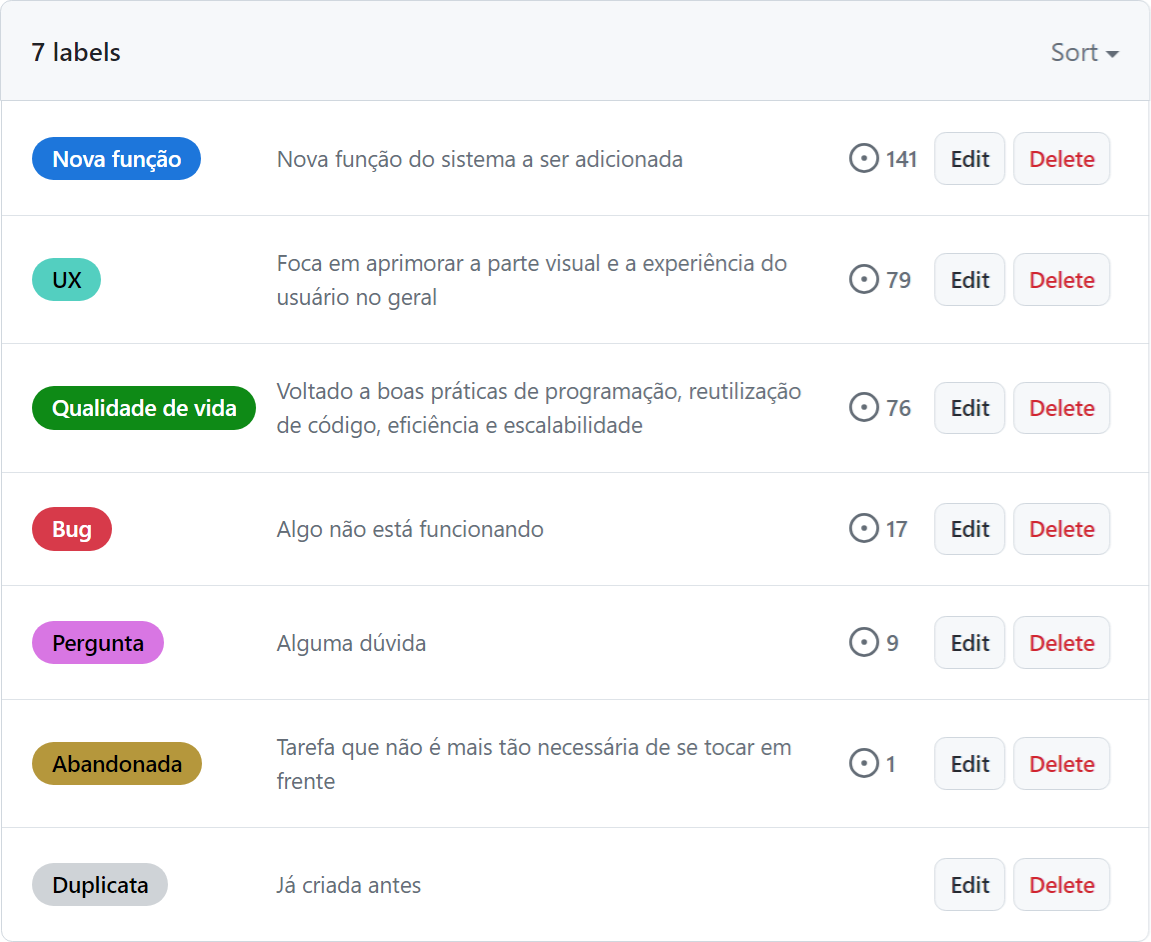
\includegraphics[width=0.7\textwidth]{files/img/2.02!5-desenvolvimento/2.02!5.4-sistema/5.4.3-MVP3/GitHubProjects-Labels-Light}
\end{MyCenteredFigure}

\begin{enumerate}
  \item \textbf{Nova função}: funcionalidades que ainda não foram implementadas;
  \item \textbf{Qualidade de vida}: melhorias que não são necessárias, mas que aprimoram o processo de desenvolvimento;
  \item \textbf{UX}: aprimoramento da experiência do usuário;
  \item \textbf{Bug}: correção de bugs;
  \item \textbf{Pergunta}: dúvidas sobre a validade da tarefa;
  \item \textbf{Abandonada}: quando criada parecia interessante, mas que se decidiu por não implementar;
  \item \textbf{Duplicata}: já foi criada antes e que foi descartada;
\end{enumerate}

\subsubsubsection*{B) Gráficos} \label{ssssec:Gráficos}

O GitHub Projects também oferece a possibilidade de visualização de gráficos na seção \textit{Insights}, que mostram a quantidade de tarefas em cada uma das categorias. Esses gráficos são úteis para a visualização do andamento do projeto, e para a identificação de possíveis gargalos. Com eles, pode-se ter uma noção das métricas do projeto, como por exemplo:

\begin{MyCenteredFigure} \caption{Gráfico de Marco \textit{versus} quantidade de tarefas separadas por etiqueta} \label{fig:ProjectsInsights}
  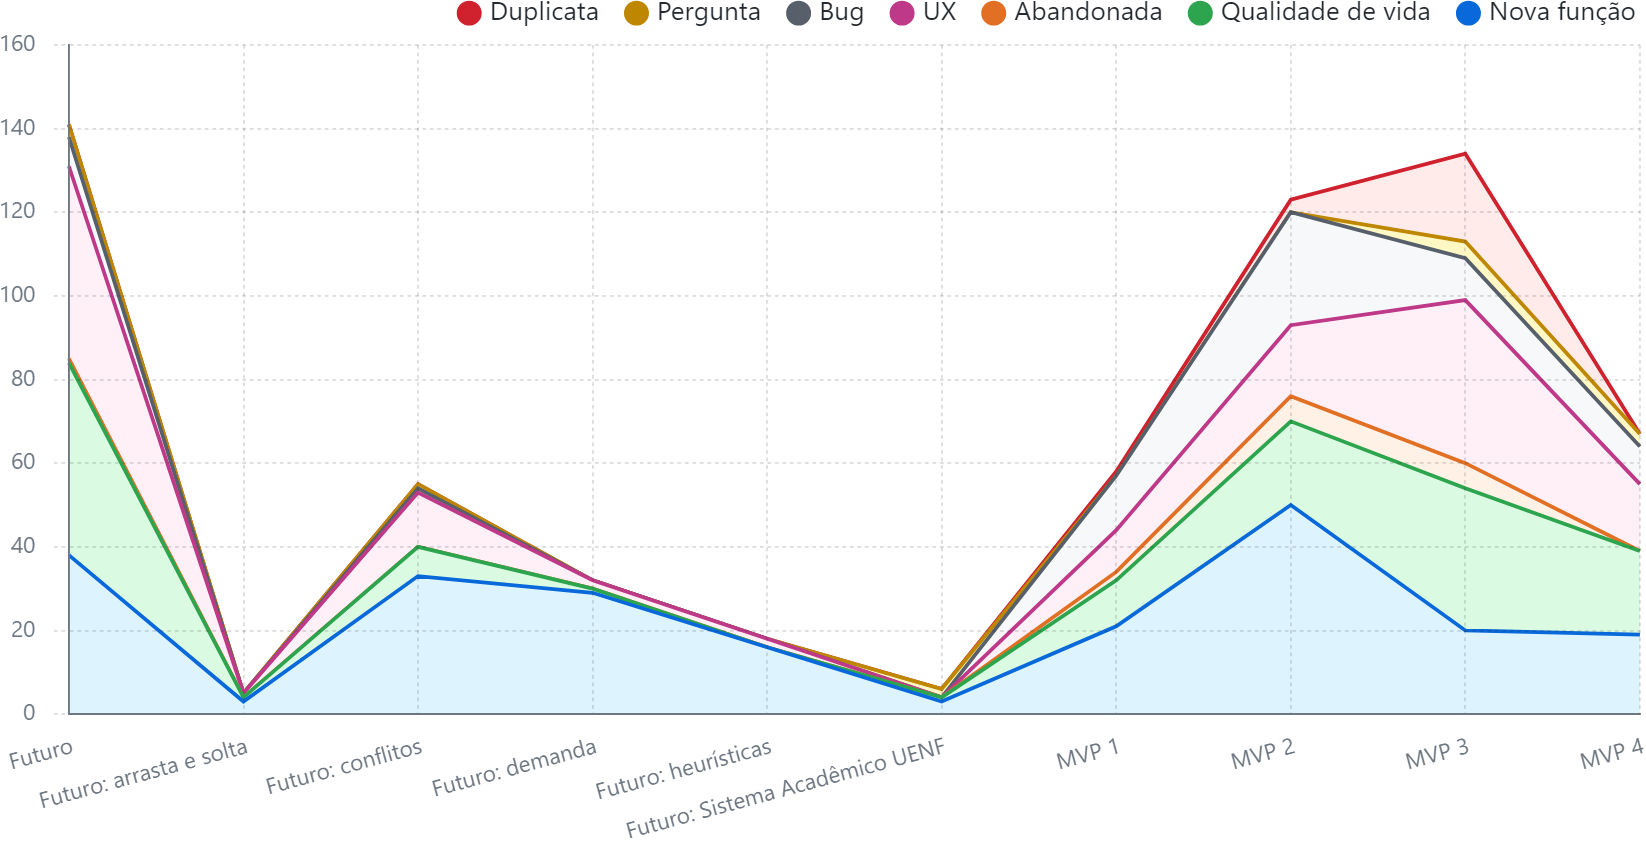
\includegraphics[width=\textwidth]{files/img/2.02!5-desenvolvimento/2.02!5.4-sistema/5.4.3-MVP3/GitHubProjects-Insights-Stacked_Line-Milestone_Label-Light}
\end{MyCenteredFigure}

\begin{itemize}
  \item Quantidade de tarefas de determinada etiqueta a cada marco, exemplificado na \autoref{fig:ProjectsInsights};
  \item Quantidade de tarefas por marco;
  \item Quais páginas receberam tarefas de quais etiquetas;
  \item Quantas são as tarefas em cada um de seus estados (\textbf{completa}, \textbf{em progresso} ou \textbf{pendente}).
\end{itemize}

\subsubsection*{\textbf{\textit{Amazon Web Services}}} \label{sssec:Amazon Web Services}

Para suprir a necessidade de um servidor que pudesse executar o \textit{backend} do sistema em conjunto com o banco de dados, foi escolhido a \textit{Amazon Web Services} (AWS). A AWS é um serviço de computação em nuvem que oferece uma ampla gama de serviços, entretanto, apenas alguns deles foram necessários para o sistema.

\begin{MyCenteredFigure} \caption{Diagrama da permanência dos dados na versão 3.0} \label{fig:API_MVP3}
  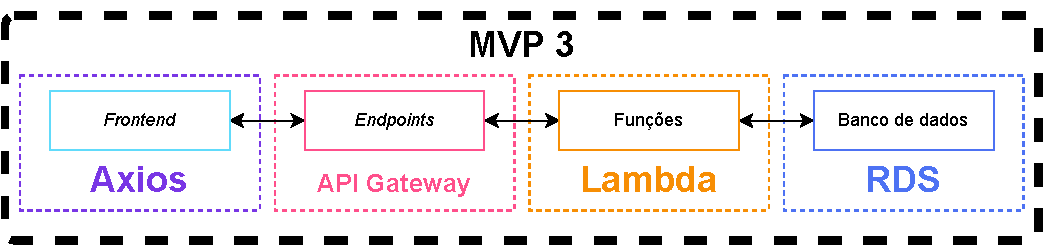
\includegraphics[width=\textwidth]{files/img/2.02!5-desenvolvimento/2.02!5.4-sistema/5.4.3-MVP3/API_MVP3}
\end{MyCenteredFigure}

O uso da AWS segue a mesma lógica do servidor local, com a diferença de que o servidor está em nuvem, e não localmente, assim resolvendo o primeiro dos dois problemas citados. Neste contexto o uso da AWS, representado pela \autoref{fig:APIAWS}, foi feito através de três serviços principais: o \textit{API Gateway} para a recepção das requisições HTTP, o \textit{Lambda} para a execução das funções que acessam o banco de dados, e o \textit{RDS} para o armazenamento dos dados; serviços estes que serão descritos mais detalhadamente a seguir. O uso desses três serviços permitiu a execução do \textit{backend} do sistema em nuvem, e assim, atingindo a permanência dos dados. Com isso, o sistema passou a ser capaz de manter os dados mesmo após a recarga da página, e assim, atender a uma das principais necessidades do sistema.

\begin{MyCenteredFigure} \caption{API REST no AWS} \label{fig:APIAWS}
  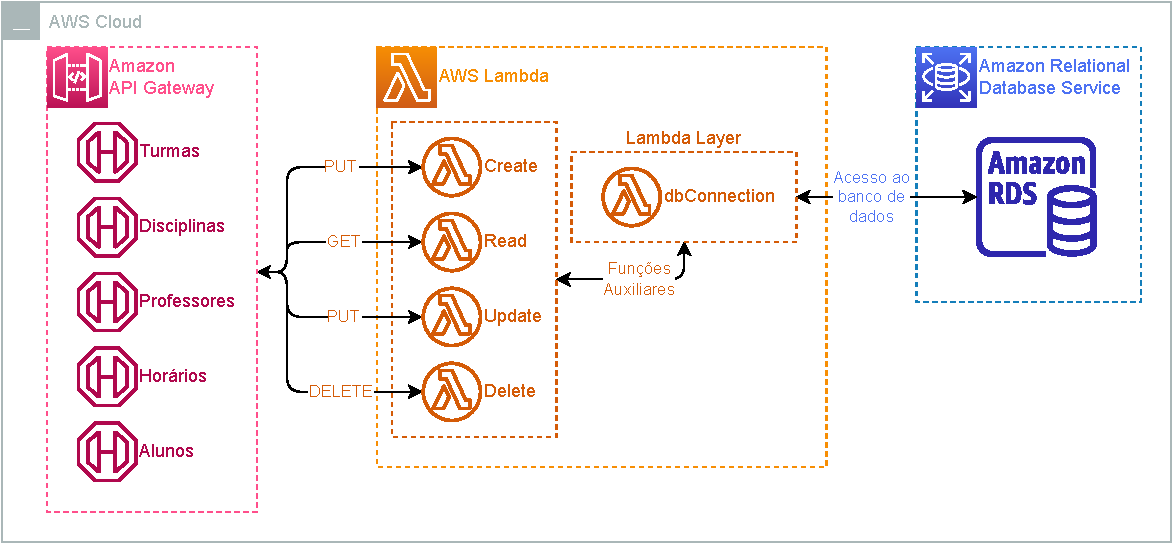
\includegraphics[width=\textwidth]{files/img/2.02!5-desenvolvimento/2.02!5.4-sistema/5.4.3-MVP3/API-Funcionamento}
\end{MyCenteredFigure}

% \subsubsubsection*{A) CORS} % Até agora não entendi direito pra que serve isso. \label{CORS}

\subsubsubsection*{A) Implantação} \label{ssssec:Implantação}

O conjunto de funcionalidades da AWS envolve em grande parte o objetivo de manter um sistema constantemente acessível através da internet, ainda assim, durante o desenvolvimento, ou até mesmo durante o ciclo de vida do software, é esperado que ocorram manutenções periódicas nas quais é compreensível que o sistema fique fora do ar. Sendo assim, para manter-se visando ao máximo a acessibilidade do sistema, espera-se que o mesmo fique desconectado o mínimo possível.

Tanto o API Gateway quanto as funções Lambda precisaram sofrer diversas modificações ao longo do desenvolvimento. A aplicação dessas modificações é chamada de implantação (\textit{deploy}), onde a AWS substitui a versão atual do sistema pela nova versão. Essa aplicação de modificações foi inicialmente feita através da interface \textit{web} da AWS, porém, com o tempo, foi percebido que essa abordagem era ineficiente. No caso das implantações do API Gateway, visto que assim que as rotas estiverem configuradas, não há a necessidade de alterá-las, não havia grande impacto no fluxo de trabalho. Já no caso das funções Lambda, cada mínima mudança no código requisitava um novo \textit{deploy} para cada uma das funções alteradas.

Outro detalhe percebido, foi que boa parte do código se repetia entre as funções que interagiam diretamente com o banco de dados. Sendo assim, passou-se a utilizar das \textit{Lambda Layers}, que são camadas que podem ser compartilhadas entre diversas funções, e assim, diminuir a quantidade de código repetido. Essa nova abordagem permitiu que as funções fossem mais enxutas, e que as mudanças fossem aplicadas de forma mais rápida, visto que bibliotecas e funções comuns entre as funções eram compartilhadas entre elas.

\subsubsubsection*{B) AWS CLI} \label{ssssec:AWS CLI}

Nas primeiras tentativas de \textit{deploy}, duas abordagens eram utilizadas: a primeira era a de copiar e colar o código diretamente na interface web da AWS, e a segunda era a de fazer o upload de um arquivo zip contendo o código.

\lstinputlisting[captionpos={t}, label={code:lambda}, caption={Código de \textit{deploy} de Lambda}]{files/codigos/AWS_CLI.sh}

Como mostrado no \autoref{code:lambda}, usa-se o software AWS CLI para criar uma função lambda. O comando \textit{create-function} é o comando que cria a função, e os argumentos que seguem são os parâmetros necessários para a criação da função. O \textit{function-name} é o nome da função, o \textit{runtime} é a versão do Node.js que a função utiliza, o \textit{role} é o conjunto de permissões criadas na seção \textit{AWS Identity and Access Management} (IAM), o \textit{handler} é o nome do arquivo principal que contém a função, e o \textit{zip-file} é o arquivo zip que contém o código da função.

Com isso, ao executar o comando, a função é criada, e então, a nova versão do código é aplicada. Com este fluxo de trabalho, embora permita o \textit{deploy} sem a direta conexão ao sistema AWS, ainda assim é necessário executar comandos específicos para cada uma, tendo que manualmente compactar o código e fazer o upload de cada um dos arquivos das diversas funções coexistentes.

\subsubsubsection*{C) SAM} \label{ssssec:SAM}

Como solução, foi utilizado o AWS SAM (\textit{Serverless Application Model}), que é uma extensão do \textit{AWS CloudFormation} que simplifica o desenvolvimento de aplicações sem servidor. O AWS SAM permite a definição de aplicações sem servidor de forma mais simples, e a partir disso, é possível fazer o \textit{deploy} de toda a aplicação de uma vez só. O uso do AWS SAM foi feito através de um arquivo \textit{template.yaml}, que contém a definição de todas as funções Lambda, e de recursos necessários para o funcionamento do sistema.

Como mostrado no \autoref{code:template} disposto no \autoref{apendice:ExemploTemplateYAML}, o arquivo \textit{template.yaml} contém a definição de algumas das estruturas utilizadas para este sistema, principalmente as funções Lambda, visto que são quatro funções para cada uma das seis entidades, totalizando 24 funções. O arquivo contém a definição de cada uma das funções, e de cada uma das rotas que elas atendem. A partir disso, é possível fazer o \textit{deploy} de todas as funções que foram alteradas de uma vez só, e assim, diminuir o tempo de \textit{deploy} e a quantidade de comandos necessários.

Após o preparativo do arquivo \textit{template.yaml}, o \textit{deploy} é feito através do conjunto de comandos \textit{sam build; sam deploy}, que primeiro combina o \textit{CloudFormation Template} com o código da aplicação, e em seguida realiza o \textit{deploy} de todas as funções definidas no arquivo. Com isso, o sistema passou a ser mais facilmente atualizável, e mais facilmente mantido.

\subsubsubsection*{D) Outros serviços da AWS} \label{ssssec:Outros serviços da AWS}

Os serviços listados até então foram os principais utilizados para a execução do \textit{backend} do sistema, entretanto, diversos outros serviços foram utilizados para a manutenção do sistema como um todo e para a execução de tarefas secundárias. Abaixo estão listados alguns desses serviços.

\begin{itemize}
  \item \textbf{S3}: serviço de armazenamento de objetos, utilizado para armazenar os objetos gerados pelo CloudFormation;
  \item \textbf{CloudWatch} e \textbf{CloudTrail}: serviço de monitoramento, utilizado para a visualização de métricas do sistema;
  \item \textbf{IAM}: serviço de gerenciamento de permissões, utilizado para a definição de permissões para as funções Lambda;
  \item \textbf{VPC}: serviço de rede privada virtual, utilizado para a definição de uma rede privada para o sistema;
  \item \textbf{Cost Explorer}: serviço de visualização de custos, utilizado para a visualização dos custos do sistema;
\end{itemize}

\subsubsection*{\textbf{Melhorias no sistema}} \label{sssec:Melhorias no Sistema}

O sistema passou por diversas pequenas mudanças, e algumas maiores. Uma considerável parte delas foi relacionada à forma com que as informações eram estruturadas internamente, mudanças essas feitas com o intuito de tornar o sistema mais fácil de ser mantido posteriormente. Em seguida estão listadas algumas das várias melhorias feitas no sistema.

\subsubsubsection*{A) Filtros e ordenações} \label{ssssec:Filtros e ordenações}

Levando em consideração a multidimensionalidade da estrutura dos dados, a possibilidade de realizar ``curvas de nível'' e as ordenar por diferentes critérios se mostrou uma funcionalidade essencial para a compreensão dos dados. Dessa forma, em diferentes páginas do sistema, foram adicionadas ordenações padrões e seletores de filtragem manual, assim permitindo ao usuário a visualização de dados específicos.

Alguns exemplos de casos de uso dessas funcionalidades seria: ``Na página \textbf{MultiTurmas} o Professor A está tendo conflitos em suas turmas, então o usuário pode filtrar as turmas do Professor A e visualizar apenas as suas turmas. Em seguida, o usuário percebe que o Professor A está em conflito com a Sala B123, então o usuário visualiza apenas as turmas da Sala B123. Por fim, o usuário encontra um outro horário disponível para o Professor A e a Sala B123, e então, o conflito é resolvido.''

Uma das solicitações presentes ao final da versão anterior foi quanto a uma distinção mais clara entre disciplinas de Ciência da Computação e disciplinas de outros cursos. Para isso, embora não pareça apresentar grande robustez na forma como foi feito, apresenta suficiente clareza para o usuário final. A distinção foi feita ao utilizar o campo \textbf{Período Esperado} presente na entidade \textbf{Disciplina}, para definir que:

\begin{itemize}
  \item \textbf{1 $\leq$ Período Esperado $\leq$ 10}: Disciplina obrigatória de Ciência da Computação;
  \item \textbf{Período Esperado = 11}: Disciplina eletiva optativa para Ciência da Computação;
  \item \textbf{Período Esperado = 12}: Disciplina eletiva livre para Ciência da Computação;
  \item \textbf{Período Esperado = 13}: Disciplina não ofertada para Ciência da Computação;
\end{itemize}

Com essa divisão, definiu-se o sistema para que, por padrão, apenas exibisse as turmas voltadas para Ciência da Computação, e que, caso o usuário desejasse, poderia visualizar as turmas de outros cursos.

\subsubsubsection*{B) MultiTurmas} \label{ssssec:MultiTurmas}

Dentre as tarefas realizadas, uma das páginas que mais sofreu alterações foi a página de \textbf{MultiTurmas}. Nela, foram feitas diversas melhorias, como a adição de filtros, ordenações e aprimoramento dos textos contidos nas caixas de seleção.

\paragraph*{B1) Adição da propriedade ``descrição''} \label{par:Descrição}

Disciplinas oferecidas em um mesmo semestre por vezes são oferecidas para alunos demais para que uma única turma os comporte, e assim, é necessário a criação de mais de uma turma. Para que os alunos e professores possam identificar facilmente a qual turma pertencem, foi adicionada a propriedade descrição, que é uma breve descrição da turma. Esse código descritor já se encontra no Sistema Acadêmico, porém com a limitação de apenas 3 caracteres. No presente trabalho, a descrição pode conter até 255 caracteres.

Adicionando esse campo, a visualização linear das informações da turma se tornou mais difícil de apresentar na tela. Considerando que em sua maioria as turmas possuem dois horários, dispôs-se então as informações em conjuntos de dois elementos, ao invés de uma lista única, tornando então a visualização mais densa.

\paragraph*{B2) Aprimoramento dos identificadores dos conflitos}

Os conflitos ocorridos indicavam quais eram os identificadores (ids) das turmas que estavam em conflito, porém, esses ids eram referentes ao banco de dados, sendo ele um valor numérico, não continha valor semântico suficiente para ser facilmente identificado. Estes ids eram visualizados ao posicionar o ponteiro do mouse por sobre os componentes cujo conflito foi verificado. Com isso, foi feita a adição de um novo identificador, que é composto pelas informações contidas na turma, sendo elas o ano, semestre, nome da disciplina, nome do professor, e o código descritor da turma. A partir disso, tornou-se mais fácil identificar quais turmas estavam em conflito, e assim, corrigi-las. Essa identificação foi adicionada também aos horários, onde o identificador passou a ser composto pela sala, dia da semana, horário de início e fim.

\paragraph*{B3) Criação e deleção de turmas e horários}

Embora seja uma funcionalidade básica e existente desde a primeira versão, a criação e deleção de turmas apresentou diversos problemas ao longo do desenvolvimento. Um dos mais cruciais era devido à assincronicidade intrínseca ao uso de um banco de dados remoto. O problema era que durante a criação sequencial de duas turmas, apenas a segunda era mostrada, mesmo que ambas tivessem sido criadas.

O que ocorria era que, ao começar com a lista de $Turmas = [A, B]$ tenta-se adicionar a turma $C$ à lista de $Turmas$, mas para isso, a requisição enviada ao banco de dados deve retornar com o status de sucesso, e para que, só assim, fosse adicionada à listagem apresentada no sistema. Então, caso fosse feita a tentativa de se adicionar a turma $D$ antes da confirmação anterior ser recebida, a adição seria realizada novamente na listagem inicial ($[A, B]$). Por fim, assim que a primeira requisição retornasse bem sucedida, por um breve instante a listagem seria $[A, B, C]$, e então, após a adição da turma $D$, a listagem seria $[A, B, D]$. Para resolver esse problema, foi feita a adição de uma função de \textit{callback} que passou a utilizar o estado mais atual da listagem de turmas, e não mais a listagem inicial.

Outra característica aprimorada, foi a velocidade de adição e deleção, principalmente a de deleção. Antes, a aprovação do banco de dados era necessária para que a lista de turmas fosse atualizada, e isso tornava o processo de deleção lento. Para resolver isso, foi feita a adição de uma função de deleção que remove a turma da listagem de turmas antes mesmo da confirmação do banco de dados. Essa não se mostra como a solução mais adequada, visto que em caso de falha na deleção, a turma poderá ser restaurada com a simples atualização da página, os pontos positivos na usabilidade superam os negativos.

\paragraph*{B4) Aprimoramento das disciplinas não oferecidas} \label{par:Solução inicial}

A funcionalidade \hyperref[sssec:Funcionalidades Adicionais]{anteriormente denominada ``Disciplinas ainda não oferecidas''} foi aprimorada de tal forma que agora, além de criar uma turma para a disciplina selecionada, o sistema automaticamente analisa o histórico de criação de turmas, definindo previamente o professor, a demanda estimada, e os horários, incluindo seus dias, horas de início e sala em que é alocada. Então, após a criação de todas as turmas referentes ao curso de Ciência da Computação, uma solução inicial foi obtida. Sendo ela mais detalhadamente descrita posteriormente na \autoref{sec:Solução inicial} denominada \nameref{sec:Solução inicial}.

\subsubsubsection*{C) Grade horária} \label{ssssec:Grade Horária}

A página que detinha o nome ``CCTable'' e que visava apresentar exclusivamente as disciplinas do curso de Ciência da Computação, foi renomeada para ``Grade Horária'', e passou a ser possível de apresentar disciplinas de todos os cursos, embora ainda não seja possível distinguir as disciplinas de um curso para o outro. As células das turmas sofreram um ligeiro aprimoramento visual e foram ordenadas primariamente por seu período esperado.

\subsubsubsection*{D) Banco de dados} \label{ssssec:Banco de dados}

Quanto ao banco de dados, os dados antes desconexos passaram a ser interligados adequadamente por chaves estrangeiras. Apresentando então restrições em casos de deleções inapropriadas no banco de dados. A API, por sua vez, deixou de retornar as listas de turmas, professores, disciplinas e salas, e passou a retornar os dados de forma mais estruturada em formato JSON.

\begin{MyCenteredFigure} \caption{Novo diagrama de banco de dados} \label{fig:MVP3_BancoDeDados}
  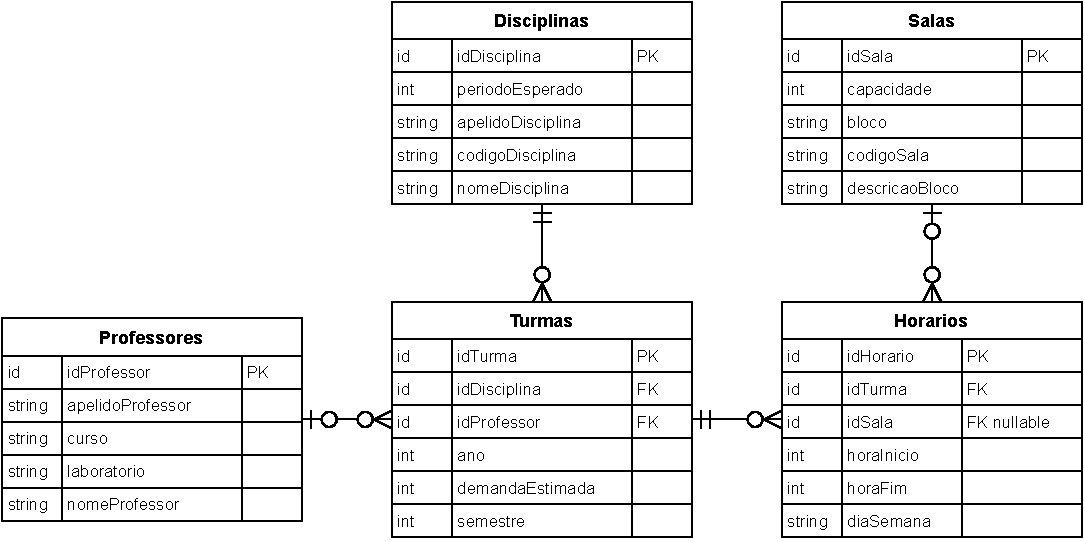
\includegraphics[width=\textwidth]{files/img/2.02!5-desenvolvimento/2.02!5.4-sistema/5.4.3-MVP3/Diagrama_ER-How_it_should_be}
\end{MyCenteredFigure}

Na \autoref{fig:MVP3_BancoDeDados} vemos as inter-relação entre as propriedades das entidades do banco de dados. Com o uso mais apropriado das chaves estrangeiras, o anterior uso dos nomes das disciplinas e professores como elementos de identificação foi substituído pelo uso de seus respectivos códigos identificadores. Houve também o surgimento da entidade \textbf{Horarios}, que interliga as turmas às salas.

\subsubsubsection*{E) Aprimoramento na forma de criação de itens}

Antes, ao acessar a página de criação de entidades, uma entidade era previamente selecionada. E para a criação de uma nova entidade, os valores da entidade anterior deveriam ser alterados, e, ao clicar em adicionar, esses valores alterados eram cadastrados no banco de dados. Essa sequência de ações não apresentou intuitividade suficiente e, portanto, foi alterada. A versão atual passou a não selecionar previamente a entidade. Assim, ao clicar em adicionar um novo item, uma nova entidade é criada. No caso das turmas, a entidade é criada com os valores de ano e semestre predefinidos baseado na filtragem selecionada.

\subsubsubsection*{F) Boas práticas}

Além das funcionalidades voltadas para o usuário final, algumas mudanças classificadas como \textbf{Qualidade de vida} foram realizadas visando a manutenção do sistema. Dentre elas estão:

\begin{itemize}
  \item \textbf{Repadronização de componentes}: como o conhecimento relacionado a boas práticas de programação foi adquirido ao longo do desenvolvimento, partes de componentes criados anteriormente foram reformulados para que estivessem estruturados de acordo com a estrutura recentemente desenvolvida no código.
  \item \textbf{Externalização de informações}: algumas informações constantes como cores de fundo e textos foram externalizadas para variáveis, assim, caso haja a necessidade de alteração, não será necessário a busca manual por todas as ocorrências. Um outro caso desses é referente aos textos dispostos nas caixas de seleção, que foram convertidos em funções que retornam o texto desejado.
  \item \textbf{Inglês}: como as linguagens de programação de modo geral se apresentam no idioma inglês, é considerado uma boa prática que as variáveis e funções também, o que não foi a abordagem inicialmente tomada. Assim, foi feita uma gradual migração para o inglês, e embora não tenha sido concluída, a maior parte do código já se encontra em inglês. Para facilitar essa migração, foi elaborado um sistema de ``\textit{getters}'' como forma de obter a propriedade de determinado objeto, independente de qual língua ele esteja.
  \item \textbf{Remoção de estruturas obsoletas}: ao longo do desenvolvimento, algumas estruturas foram criadas e não utilizadas. Um exemplo dessas foi a propriedade ``Ordem'' que visava definir a ordem em que os horários da turma apareceriam, porém o resultado desta propriedade foi obtido com a ordenação dos horários por dia e em seguida por horário, não sendo então necessária. Ela então foi removida do sistema e do banco de dados.
\end{itemize}

\section{Solução inicial} \label{sec:Solução inicial}                                   % ###  5.5 

Um dos processos mais importantes para a alocação de turmas é a definição de uma solução inicial. Ao longo das versões, a solução inicial foi sendo aprimorada, deixando de \hyperref[sssec:Funcionalidades Adicionais]{criar turmas para todas as disciplinas disponíveis, porém sem as suas informações preenchidas}, para \hyperref[par:Solução inicial]{criar turmas com suas características já preenchidas seguindo uma heurística baseada no histórico de criação de turmas}.

O botão de adição de todas as disciplinas foi mantido, e agora, ao ser clicado, cria as turmas com suas características já preenchidas, assim gerando uma solução inicial, porém passível de conflitos. Vale ressaltar que o preenchimento das características, entretanto, não inclui a propriedade \hyperref[par:Descrição]{descrição}, visto que esta é uma característica única de cada turma e deve ser adicionada manualmente somente em caso de necessidade.

\subsection{Heurística histórica para criação de uma solução inicial} \label{ssec:Heurística}

A solução inicial é obtida através de uma heurística própria que analisa o histórico de criação de turmas com o objetivo de criar todas as turmas necessárias para o semestre. O histórico em que se baseia consiste em todas as turmas, de todos os anos, cadastradas no sistema, sendo elas do curso de Ciência da Computação ou não. A partir disso, define as características das turmas a serem criadas. A heurística é executada assim que o botão de adição de turmas a partir das disciplinas ainda não ofertadas for clicado.

Baseado na grade curricular de 2015, foram armazenadas no sistema as disciplinas e seus respectivos períodos esperados. Com essa informação, é possível distinguir entre disciplinas geralmente oferecidas no primeiro semestre (aquelas cujo período esperado é um número ímpar), e as disciplinas oferecidas no segundo semestre (aquelas cujo período esperado é um número par).

Na seção inferior da página Multiturmas há uma tabela com a listagem das disciplinas esperadas a serem oferecidas no semestre selecionado nos filtros, desde que ainda não tenham sido atreladas a alguma turma naquele semestre. Listagem essa que apresenta as disciplinas pares, ímpares, ou todas, caso o semestre de verão seja selecionado.

Com essas informações o usuário pode escolher criar uma turma para uma \textbf{disciplina em específico}, ou então uma turma para \textbf{cada uma das disciplinas listadas}. Ao criar uma turma para uma \textbf{disciplina específica}, ele inserirá essa disciplina em uma lista de turmas a serem criadas. Já ao criar uma turma para \textbf{todas as disciplinas listadas}, o sistema irá inserir todas as disciplinas da listagem em uma lista de turmas a serem criadas.

A partir daí o sistema percorrerá cada uma das disciplinas na listagem das turmas a serem criadas e, filtrará do cadastro histórico de turmas para que sejam obtidas \textbf{apenas as turmas da disciplina em questão}. Em seguida, a heurística analisa a listagem das turmas já filtradas e define as características das turmas a serem criadas.

O algoritmo de aquisição das informações para a criação da turma é ilustrado no \autoref{code:heuristica} e consiste em 4 funções principais: \textit{splitClasses}, \textit{getMostFrequentClassTimeSizes}, \textit{getMeanDemand} e \textit{getMostFrequent}.

\begin{lstlisting}[language=JavaScript, caption={Heurística de solução inicial}, label={code:heuristica}]
function getUsualInfo(classes) {
  const classTimes = splitClasses(classes);
  const quantity = getMostFrequentClassTimeSizes(classes);
  const classUsualInfo = {
    professor: getMostFrequent(classes, ["professor"]),
    expectedDemand: getMeanDemand(classes),
    // description: getDescription(classes, currentSemester),
    description: null,
    classTime: {
      quantity,
      day: getMostFrequent(classTimes, ["dia"], quantity),
      room: getMostFrequent(classTimes, ["sala"]),
      duration: getMostFrequent(classTimes, ["duracao"]),
      startHour: getMostFrequent(classTimes, ["horaInicio"]),
    },
  };
  return classUsualInfo;
}
\end{lstlisting}

Na função \textbf{\textit{splitClasses}} uma lista de objetos ``turma'' contendo múltiplos horários é passada por parâmetro e é dividido em uma lista de objetos ``turma'', onde cada objeto contém as informações de um dos horários, então retornando uma lista de objetos ``horário''. Essa função realiza esta conversão para que se possa trabalhar com os dados referentes a cada horário de forma individual.

Na função \textbf{\textit{getMostFrequentClassTimeSizes}} é passada uma lista de objetos ``turma'' contendo múltiplos horários e é retornado um número inteiro que representa a quantidade de horários que foi mais frequente dentre as turmas passadas por parâmetro. Essa função é utilizada para definir a quantidade de horários que a nova turma terá.

Na função \textbf{\textit{getMeanDemand}} é passada uma lista de objetos ``turma'' e é retornado um número inteiro que representa a média da demanda de todas as turmas que possuam demanda estimada.

Na função \textbf{\textit{getMostFrequent}} são passados três parâmetros usualmente: uma \textbf{lista de objetos} ``turma'' ou uma lista de objetos ``horário'', uma lista de strings que representam \textbf{o campo que se deseja analisar}, e um número inteiro que representa a \textbf{quantidade de valores} que se deseja retornar, sendo este valor igual a 1 caso nenhum valor seja passado. A função então usa a lista de objetos passada por parâmetro para contar a frequência de cada valor registrado no campo desejado, e então, retorna os valores mais frequentes.

Com essas quatro funções são coletadas as informações pertinentes à turma de tal disciplina, sendo elas: professor, demanda estimada, quantidade de horários, dia, sala, duração e hora de início. E, com esses dados, o sistema criará uma turma para a disciplina em questão contendo as informações obtidas.

\subsection{Requisitos, benefícios e limitações da heurística histórica} \label{ssec:limitacoes_heuristicas}

Como a heurística é baseada no histórico de criação de turmas, é necessário, claro, que haja um histórico de criação de turmas para que a solução inicial seja obtida. E, quanto maior o histórico, mais precisa será a solução inicial obtida.

A heurística é capaz de prever com certa precisão as características das turmas a serem criadas. Entretanto, a solução encontrada está passível de apresentar conflitos visto que nem todas as alocações de turmas apresentam um padrão objetivo. Além disso, a heurística não checa se a turma a ser criada está alocada em um horário já ocupado pelo professor ou sala em questão. Outra limitação é quanto a professores que já não estejam mais associados à instituição ou que acabaram de ser contratados, nesses casos, os mesmos, devido à baixa frequência de alocações, terão menor probabilidade de serem alocados.

Como o usuário tem a capacidade de escolher alocações de apenas algumas disciplinas específicas, a geração da solução inicial pode ser feita parcialmente, o que traz maior flexiblidade ao usuário.

As limitações da heurística encarregam então ao usuário a verificação e a correção dos possíveis conflitos gerados durante a criação da solução inicial. Essa correção se dá através da análise do sistema de \hyperref[sec:conflitos]{detecção e alerta dos conflitos}.

\section{Detecção e alerta dos conflitos} \label{sec:conflitos}                         % ###  5.6

Uma das principais funcionalidades do sistema é a detecção de conflitos. Seu objetivo é auxiliar ao usuário a identificar possíveis problemas na alocação das turmas, e assim, permitir que ele possa corrigi-los antes de finalizar a grade horária. Diversas situações podem ser consideradas como conflitos, e cada uma delas é tratada de forma diferente.

Os conflitos aqui se colocam como uma forma de alerta ao usuário, e não como uma restrição, assim viabilizando ao usuário que uma ação seja tomada, ou não, a partir do alerta. O conceito da não restrição é importante, visto que embora idealmente espera-se que o processo de alocação disponha de todas as informações para que seja otimamente alocado, na prática, isso atualmente não se mostra uma realidade.

Essa flexibilização das restrições que poderiam ser tidas como rígidas em um problema de otimização, é uma característica do problema de alocação de turmas da UENF. Como na realidade da instituição as grades precisam ser criadas enquanto ainda se tem informações incompletas, certas decisões precisam ser tomadas manualmente, sendo então necessária esta flexibilidade para permitir que o usuário possa tomar essas decisões.

Além disso, diversos casos atípicos acabam por ocorrer na realidade da universidade, e que, embora possam não ser aconselháveis ou até mesmo tidos como conflituosos pelo sistema, não seriam de fato um problema para a execução prática das alocações.

\subsection{Conflitos atípicos}

Nessa seção são descritos alguns exemplos de conflitos que poderiam ser alertadas pelo sistema, mas que não seriam realmente um restritor para a execução prática das alocações.

Considerando o corpo docente do curso de Ciência da Computação, que atualmente conta com seis professores doutores, é recorrente a solicitação de professores bolsistas para ministrar disciplinas. Devido aos prazos existentes ao longo do processo de criação da grade horária, é comum que ainda não se saibam quais e quantos professores bolsistas serão disponibilizados para quais turmas. Porém, como o Sistema Acadêmico requere a inserção de professores para a criação de turmas, uma solução encontrada foi a inserção de um desses professores permanentes como responsável pela turma. E, mesmo após se obter a informação quanto a quais e quantos bolsistas estarão disponíveis, ainda assim o sistema acadêmico não os permite serem inseridos, visto que eles não têm um vínculo permanente com a instituição. Com isso, seria possível ver, por exemplo, um conflito entre duas turmas que possuem o mesmo professor em um mesmo horário, mas que na prática, uma delas será ministrada por um professor bolsista.

Outras situações que podem ocorrer giram em torno da alocação das salas. Duas situações que podem ilustrar sua atipicidade são: a possibilidade de alocar uma turma a uma determinada sala, mesmo que se tenha a intenção de ministrá-la em outra, e também a possibilidade de se repartir a turma em duas salas de aula ocorrendo simultaneamente.

\subsection{Conflitos tratados pelo sistema} \label{ssec:ConflitosTratados}

Para a implementação, primeiro visou-se a detecção de conflitos que poderiam ser considerados restritores para a alocação das turmas. Sendo eles os de alocação simultânea de salas e professores, visto que um professor não pode ministrar em duas turmas simultaneamente, nem uma sala deve comportar duas turmas simultaneamente (embora ambos sejam teoricamente possíveis). Além disso, também foi implementada a detecção de conflitos de capacidade, onde a quantidade de alunos de uma turma é maior do que a capacidade da sala alocada, e alguns outros indicativos visuais que serão descritos abaixo.

Os conflitos calculados são representados de três formas diferentes. A primeira e mais perceptível é a mudança de cor de fundo dos atributos conflituosos. A segunda, visando evitar sobreposição de conflitos, é a adição de uma borda inferior que se estende por toda a largura do atributo. E a terceira, mais descritiva, é o uso do atributo \textit{title} dos elementos HTML, que exibe uma mensagem de alerta flutuante ao passar o mouse sobre o atributo conflituoso, assim dispondo de mais detalhes sobre os conflitos buscados e encontrados.

Embora o sistema seja projetado para ser permissivo quanto a inexistência de certas informações, é sempre esperado que a maior quantidade de informações possíveis seja inserida, assim, caso algum campo não tenha sido preenchido a cor de fundo do elemento será alterada para um tom acinzentado.

\begin{MyCenteredFigure} \caption{Paleta de cores do sistema} \label{fig:conflitoDisciplinaPaleta}
  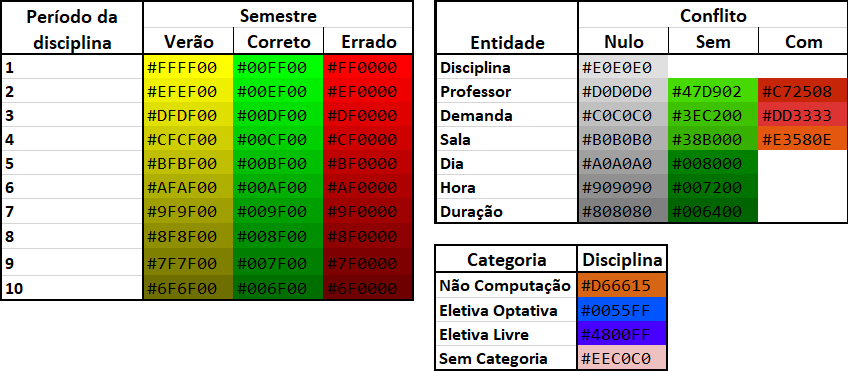
\includegraphics[width=\textwidth]{files/img/2.02!5-desenvolvimento/2.02!5.6-conflitos/Paleta de Cores}
\end{MyCenteredFigure}

Os conflitos que são representados por cores, têm sua paleta de cores representada na \autoref{fig:conflitoDisciplinaPaleta}. Nessa paleta, dispõe-se 3 conjuntos principais: a distribuição de cores para as disciplinas obrigatórias do curso de Ciência da Computação, que variam de acordo com o semestre em que são ofertadas; a categoria das disciplinas não obrigatórias para o curso de Ciência da Computação; e os conflitos das outras entidades, que são classificados amplamente entre ``com conflito'', ``sem conflito'' e ``conflito nulo'' (dados faltantes).

Cinco campos se encontram sem cores, sendo eles a \textbf{Disciplina sem conflito}, \textbf{Disciplina com conflito}, \textbf{Dia com conflito}, \textbf{Hora com conflito} e \textbf{Duração com conflito}. No caso dois dois primeiros, melhor explicado \hyperref[sssec:Disciplina]{a seguir}, a representação dos conflitos é substituída pela representação de seu período esperado e de suas categorias. Já os três últimos também não possuem conflitos por si só, o que ocorre é que herdam a cor de fundo das entidades que têm conflito em determinado dia, hora e duração, como é o caso da alocação múltipla de turmas em uma mesma sala ou de professores em turmas simultâneas.

\begin{MyCenteredFigure} \caption{Exemplo de conflito nulo} \label{fig:turmaVazia}
  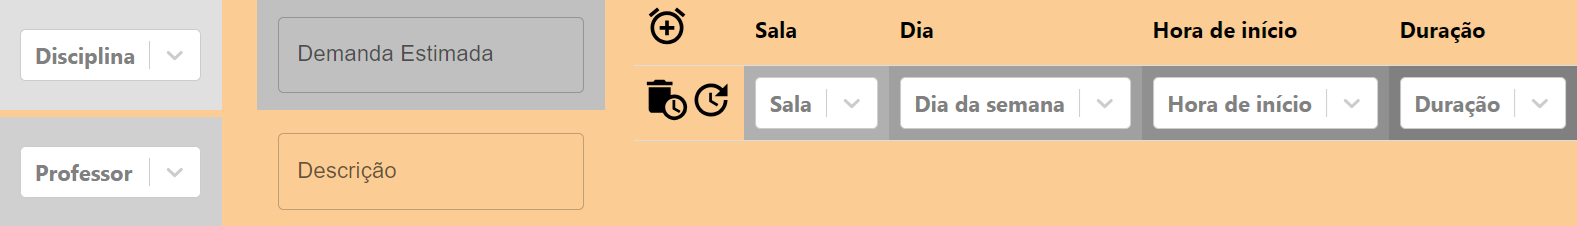
\includegraphics[width=\textwidth]{files/img/2.02!5-desenvolvimento/2.02!5.6-conflitos/Incompletude de informações}
\end{MyCenteredFigure}

A \autoref{fig:turmaVazia} ilustra os \textbf{conflitos nulos}. Esse tipo de conflito representa a incompletude de informações, e como durante parte do processo de criação da grade não se tem todas as informações sobre as alocações das turmas, ele acaba por ser um dos conflitos mais comuns. Esse conflito, representado pela cor acinzentada, é detectado quando um dos campos não se encontra preenchido.

\subsubsection*{\textbf{Conflitos de professores}} \label{sssec:Professores}

O sistema contempla a checagem de conflitos de alocação simultânea de professores em mais de uma turma. Ou seja, considerando todas as turmas às quais o professor está atribuído no ano e semestre selecionados, o sistema compara todos os horários das turmas deste professor, e verifica se há alguma interseção entre horários que estão no mesmo dia, levando em conta a duração da aula.

\begin{MyCenteredFigure} \caption{Exemplo de conflito de alocação de professor} \label{fig:conflitoAlocacaoProfessor}
  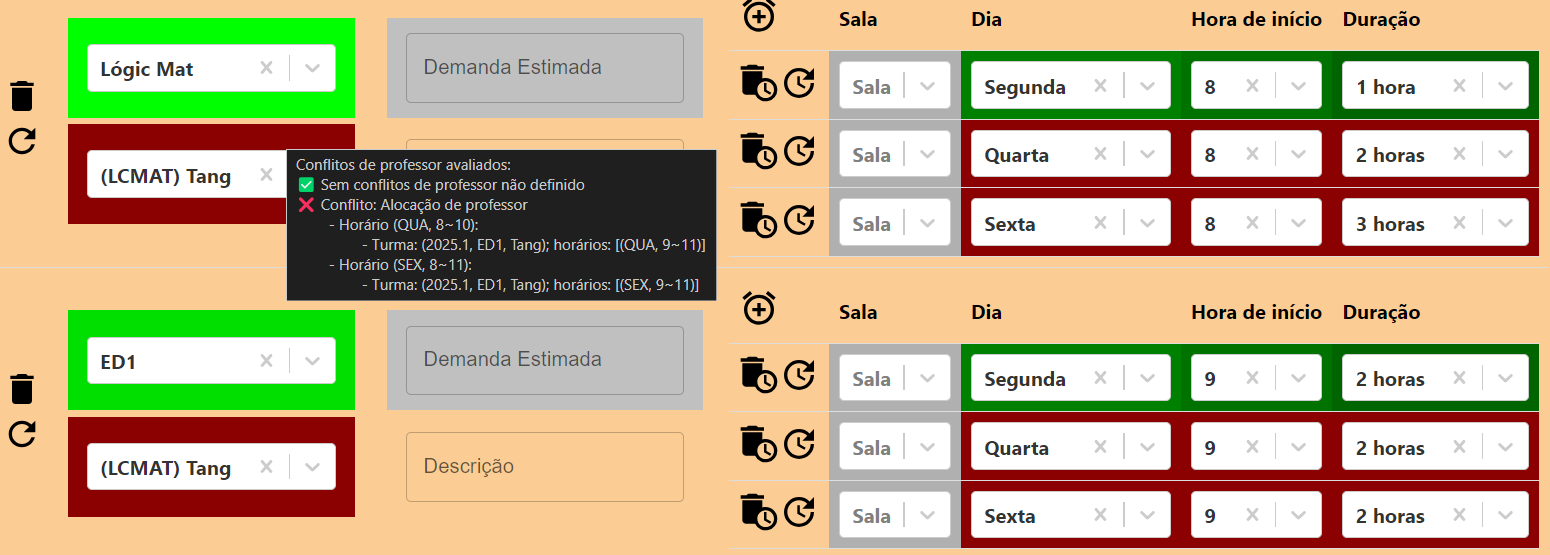
\includegraphics[width=\textwidth]{files/img/2.02!5-desenvolvimento/2.02!5.6-conflitos/Alocação de professores}
\end{MyCenteredFigure}

Caso haja algum conflito, o sistema destaca o professor em questão, tornando a sua cor de fundo avermelhada. Além disso, ao passar o mouse sobre o nome do professor, é exibido um alerta flutuante, informando quais são as turmas e horários que estão em conflito. Esse comportamento é exemplificado na \autoref{fig:conflitoAlocacaoProfessor}, onde o professor Tang é alocado em duas turmas que ocorrem simultaneamente durante algum intervalo de tempo durante os horários de quarta e sexta-feira, assim informando no alerta flutuante quais são as turmas e horários que estão alocados simultaneamente.

\subsubsection*{\textbf{Conflitos de salas}} \label{sssec:Salas}                                 % #### 5.6.1

\begin{MyCenteredFigure} \caption{Exemplo de conflito de alocação de sala} \label{fig:conflitoAlocacaoSalas}
  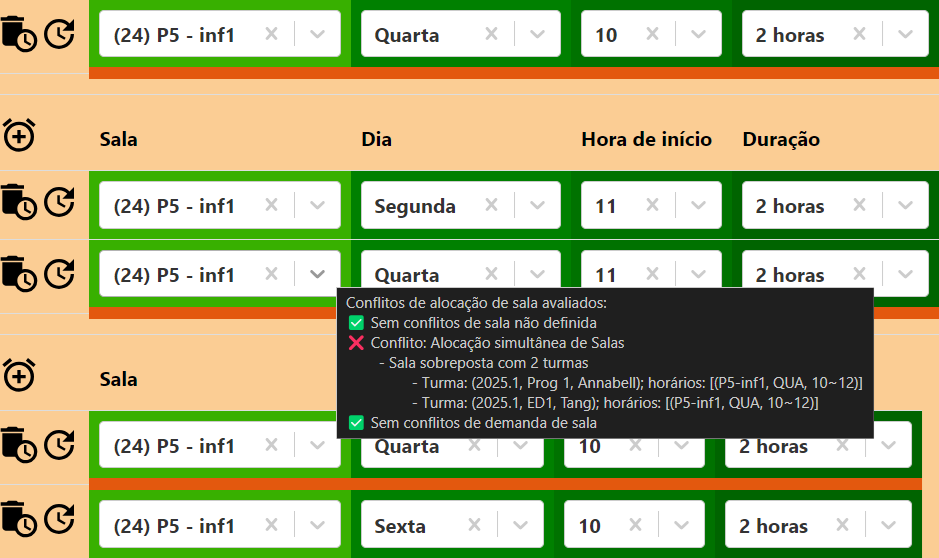
\includegraphics[width=\textwidth]{files/img/2.02!5-desenvolvimento/2.02!5.6-conflitos/Alocação de Salas - Sala}
\end{MyCenteredFigure}

As salas também apresentam a verificação do conflito de alocação simultânea. Porém, diferente dos professores, a checagem é feita conferindo todos os horários na qual a sala está alocada, e então é feita a mesma verificação de interseção citada anteriormente. Havendo o conflito, é exibida uma borda alaranjada na parte inferior das propriedades referentes ao conflito, além de, assim como no caso dos professores, exibir o alerta flutuante. A \autoref{fig:conflitoAlocacaoSalas} representa um caso de conflito de alocação de salas.

\begin{MyCenteredFigure} \caption{Exemplo de conflito de capacidade na sala} \label{fig:conflitoAlocacaoSalasCapacidade}
  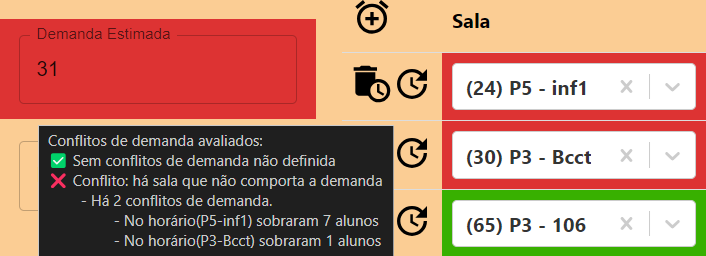
\includegraphics[width=\textwidth]{files/img/2.02!5-desenvolvimento/2.02!5.6-conflitos/Demanda X Capacidade}
\end{MyCenteredFigure}

Além disso, também é feita a comparação entre a quantidade máxima de alunos comportados na sala e a quantidade de alunos estimados para a turma. Este conflito por sua vez é ilustrado tornando avermelhado o fundo da demanda estimada e da seleção de salas. Caso uma turma tenha mais de um horário, é calculada a quantidade remanescente dos alunos que demandam a disciplina com relação a cada uma das capacidades das salas destes horários, mostrando cada um deles no alerta flutuante.

Então, como pode-se perceber na \autoref{fig:conflitoAlocacaoSalasCapacidade}, a turma ilustrada apresenta demanda estimada de 31 alunos não poderia ser adequadamente alocada às salas ``P5 - inf1'', nem na ``P3 - Bcct'', visto que a primeira apenas comporta 24 alunos e a segunda, 30 alunos. O alerta flutuante, ao ser acionado, informa ainda quantos são os alunos que não poderiam ser alocados em cada uma das salas.

\subsubsection*{\textbf{Conflitos de disciplina}} \label{sssec:Disciplina}                       % #### 5.6.2

\begin{MyCenteredFigure} \caption{Avisos flutuantes dos conflitos de disciplinas A} \label{fig:conflitoDisciplinaTitulos_A}
  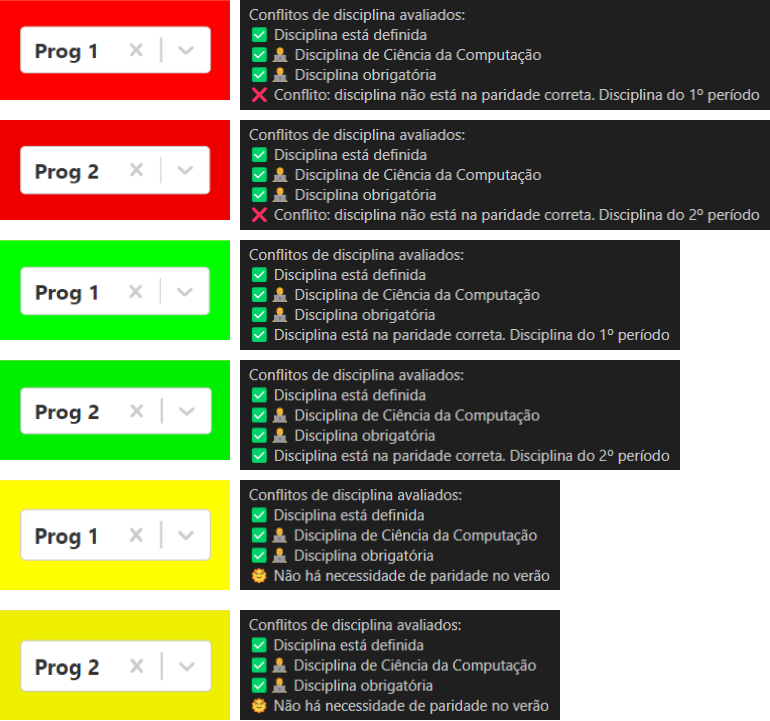
\includegraphics[width=0.8\textwidth]{files/img/2.02!5-desenvolvimento/2.02!5.6-conflitos/Categorias Disciplinas A}
\end{MyCenteredFigure}

Além desses conflitos, outras características analisadas e representadas se referem às disciplinas atribuídas às turmas, que, embora não representem necessariamente um \textit{conflito}, mas sim um indicativo, ainda assim serão tratados como conflitos por motivos de simplificação. Esse indicativo leva em consideração o semestre selecionado e o período esperado da disciplina de certa turma. Utilizando de lógica similar, também é indicado caso não tenha sido atribuído um período à disciplina, e se, para o curso de Ciência da Computação, a disciplina é considerada como \textbf{Eletiva Livre}, \textbf{Eletiva Optativa}, ambas em tons azulados, ou se não é uma disciplina para o curso de Ciência da Computação, sendo então representada em tons alaranjados. Estas características são ilustradas no lado direito da \autoref{fig:conflitoDisciplinaTitulos_A}.

\begin{MyCenteredFigure} \caption{Avisos flutuantes dos conflitos de disciplinas B} \label{fig:conflitoDisciplinaTitulos_B}
  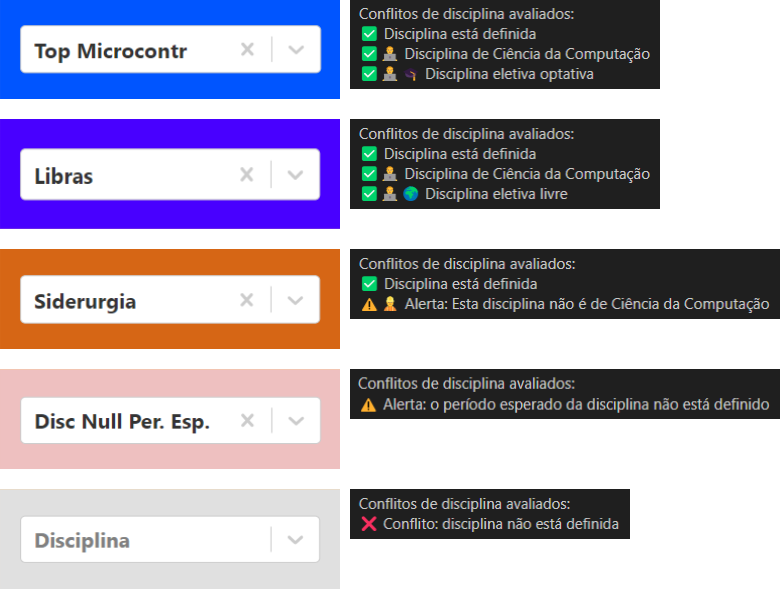
\includegraphics[width=0.8\textwidth]{files/img/2.02!5-desenvolvimento/2.02!5.6-conflitos/Categorias Disciplinas B}
\end{MyCenteredFigure}

Já no lado esquerdo da \autoref{fig:conflitoDisciplinaTitulos_B}, vemos os conflitos que correlacionam os períodos esperados das disciplinas obrigatórias do curso de Ciência da Computação com o semestre em que foram ofertadas. Os semestres possíveis são três: o primeiro semestre, o segundo semestre e o ``período de verão''. No caso do período de verão, as disciplinas que têm o seu período esperado neste semestre são marcadas com um tom amarelado, visto que não há relevância da sua paridade em um período de férias. Já nos casos das disciplinas de paridade ímpar (disciplinas dos períodos 1, 3, 5, 7 e 9) no primeiro semestre, ou as disciplinas de paridade par (disciplinas dos períodos 2, 4, 6, 8 e 10) no segundo semestre, estas são marcadas com um tom esverdeado, sendo aquelas referentes aos períodos finais do curso marcadas com um tom mais escuro. Já as disciplinas pares em semestres ímpares, ou as disciplinas ímpares em semestre pares, são ilustradas com a cor avermelhada, seguindo a mesma lógica de gradiente escuro nos últimos períodos.

\subsection{Resolução dos conflitos} \label{ssec:Resolução}                             % #### 5.6.3

A resolução dos conflitos é feita de forma manual, e o sistema não apresenta uma funcionalidade que permita a resolução automática dos conflitos. A resolução é feita através da análise dos alertas flutuantes e das cores identificadoras dos conflitos, e então, a partir disso, o usuário pode tomar a ação necessária para a resolução dos conflitos. A sequência de ações necessária para a resolução dos conflitos é arbitrária aos gostos do usuário, sendo fortemente dependente da subárea do problema que o usuário deseja resolver. Ainda assim, de forma geral é listado no \autoref{code:pseudo} um pseudo-algoritmo que descreve uma possível sequência para a resolução dos conflitos.

\begin{lstlisting}[language=Python, caption={Pseudo-algoritmo para a resolução de conflitos}, label={code:pseudo}]
def resolveConflitos():
  while ha_informacoes_faltantes():
    adicione_informacoes_faltantes()
    while ha_conflitos():
      ordene_tipos_de_conflitos_por_prioridade()
      for tipo_de_conflito in tipos_de_conflitos:
        conflitos_selecionados = selecione_conflitos(tipo_de_conflito)
        for conflito in conflitos_selecionados:
          analise_grade_horaria_da_entidade_em_questao(conflito)
          realocar_entidade_para_onde_nao_haja_conflito()
\end{lstlisting}

\begin{comment}
Início
Enquanto (a grade estiver incompleta) faça:
Adicione as informações faltantes
Enquanto (houver conflitos) faça:
Ordenar tipos de conflitos por prioridade
Para cada (tipo de conflito) faça:
Selecionar todos os conflitos desse tipo
Para cada (conflito) faça:
Analisar a grade horária da entidade em questão
Alocar a entidade a um novo conjunto de variáveis que não gere conflito
Fim Para
Fim Enquanto
Fim Enquanto
Fim
\end{comment}

\section{Preenchimento de dados} \label{sec:preenchimento}                              % ###  5.7

Inicialmente, os dados adicionados faziam jus diretamente às disciplinas, professores, salas e turmas do curso de Ciência da Computação. Porém, como para a análise completa dos conflitos é necessário que seja feita também a adição das turmas de outros cursos, foi feito o preenchimento de dados para as entidades de professores, disciplinas e salas.

Para acumular mais dados referentes às entidades do banco de dados, foram tomadas algumas abordagens: requisição dos dados diretamente do Sistema Acadêmico, processamento de tabelas, processamento de PDFs e \textit{web scraping}, todos eles ilustrados pela \autoref{fig:DataFlow}.

\begin{MyCenteredFigure} \caption{Diagrama do fluxo de obtenção de dados} \label{fig:DataFlow}
  \includegraphics[width=\textwidth]{files/img/2.02!5-desenvolvimento/2.02!5.7-preenchimento/Processamento de dados}
\end{MyCenteredFigure}

A forma teoricamente mais direta e eficiente para se obter os dados das entidades é a obtenção das informações contidas no banco de dados do sistema acadêmico. Para este fim, foi feita uma solicitação ao responsável pela Secretaria Acadêmica (SECACAD) da UENF, que direcionou a solicitação ao desenvolvedor do Sistema Acadêmico. A resposta obtida do desenvolvedor foi que a solicitação não poderia ser atendida, visto que não detinha a posse dos dados, e que para que pudesse fornecê-los, seria necessária uma solicitação formal à reitoria da UENF. Essa solicitação foi então passada à Coordenação do curso de Ciência da Computação, com o qual ficou decidido abandonar a ideia e buscar outras formas de obtenção dos dados.

Paralelamente à abordagem anterior foram feitas tentativas individuais de obtenção dos dados. O processamento de tabelas e PDFs e o \textit{web scraping} foram as abordagens utilizadas. Inicialmente os dados foram coletados e armazenados em tabelas, e então, convertidos para o formato CSV. Os arquivos CSV, por sua vez, foram utilizados em \textit{scripts} Python que os convertiam em \textit{queries} SQL, para que assim então fossem adicionados ao banco de dados.

Os PDFs analisados dispunham de tabelas referentes à oferta de turmas para o CCT, mas os dados advindos do processamento de PDF não são tão estruturados quanto os de uma tabela Excel, por este motivo, a primeira abordagem foi a solicitação dos arquivos tabulares para aquele que os produziu. Não havendo resposta favorável quanto a isso, diversos \textit{softwares} de conversão de tabelas em PDF para Excel foram testados, porém, nenhum deles foi capaz de converter as tabelas de forma satisfatória. Um dos agravantes é a existência de células mescladas, o que torna mais complicada a conversão direta. Outra abordagem testada foi a de importação direta dos PDFs através do Excel e também o simples copiar e colar. Nenhum desses métodos foi eficiente, então com isso alguns dados foram coletados, mas sem certeza quanto à sua precisão. Deste método foram coletadas as informações referentes à nomes de professores e disciplinas, capacidades das salas, e horários de aulas.

Além dos PDFs anteriores, haviam também os arquivos referentes à oferta de turmas para o curso de Ciência da Computação. Estes sim dispunham também de sua versão em Excel, e assim, foram processados utilizando \textit{scripts} Python. A abordagem apresentou falhas, visto que a notação das informações não apresentava o mesmo padrão ao longo dos anos, então foi necessário fazer ajustes manuais, resultando em uma tabela normalizada com diversas pastas de trabalhos referentes a cada um dos semestres desde 2019, não considerando os semestres de verão. Deste método foram coletadas as informações referentes à nomes e apelidos de professores e disciplinas, demandas estimadas dos alunos pela turma, descrição da turma, e horários de aulas.

Por fim, foi feita o \textit{web scraping} que consistiu na busca por informações em diversos sites, principalmente o \LinkToURL{\LinkAcademicoUENF}{Sistema Acadêmico}, o \LinkToURL{\LinkSiteUENF}{site da UENF} e outros sites. Nessa etapa, foi possível encontrar lotes de informações estruturadas. Um dos lotes foi a listagem de disciplinas e suas características que se encontram disponíveis no Sistema Acadêmico da UENF, essas informações foram copiadas e coladas no arquivo Excel unificado. Outros lotes foram encontrados dispersos ao longo do site da UENF e consistiam basicamente em listagem de professores e seus respectivos laboratórios. Essas informações estavam dispersas dos sites dos diversos centros e cursos, alguns disponíveis no próprio site, outros em formato de arquivo. Deste método foram coletadas as informações referentes à nomes de professores, seus laboratórios e centros; e disciplinas e seus nomes, códigos e períodos de vigência. Além disso, foram encontrados documentos oficiais que referenciam a capacidade de ocupantes das ``salas'' disponíveis do Centro de Convenções, popularmente conhecido como ``Apitão'' que mesmo não sendo propriamente uma sala de aula, já foi utilizado previamente para tal fim. Outras salas já obtiveram alocações similares, assim como a Sala dos Professores.

\section{Próximos desenvolvimentos} \label{sec:proximos}                                % ###  5.8

Ao longo de todo o desenvolvimento, podemos dividir as funcionalidades em quatro categorias: as que foram \textbf{implementadas e se mantiveram}, as que foram \textbf{implementadas e descartadas}, as que \textbf{não foram implementadas} e as que foram \textbf{preparadas} para próximos desenvolvimentos.

As \textbf{implementadas e se mantiveram} são aquelas principais e essenciais para o funcionamento do sistema, como a adição de turmas, professores, disciplinas e salas, a visualização da grade horária, a detecção de conflitos.

As \textbf{implementadas e descartadas} são aquelas que por diversos motivos, não se mantiveram no sistema. Um exemplo disso é a funcionalidade de travamento de turmas, que foi implementada, mas descartada por não ser considerada essencial.

As \textbf{não implementadas} são aquelas que, devido a priorização das tarefas, não detiveram importância o bastante para que chegassem à etapa de implementação. Um exemplo disso é a funcionalidade de alterar a grade horária através do sistema de arrastar e soltar.

As \textbf{preparadas mas não implementadas} são aquelas que, por conveniência ou por praticidade do momento, foram parcialmente desenvolvidas, mesmo que não tenham grande participação no sistema final. Dentre elas, podemos citar a funcionalidade de adição de alunos, e diversas tabelas e colunas no banco de dados que foram criadas e preenchidas mas não utilizadas.

\subsection{Funcionalidades preparadas} \label{ssec:Funcionalidades preparadas}         % ###  5.8.1

Dentre as funcionalidades preparadas temos o sistema de cadastro de alunos, que consiste basicamente na adição das informações básicas dos alunos, como ano de entrada, curso, matrícula e nome como é visto em sua tabela no canto inferior direito na \autoref{fig:DER final}. Seus dados podem ser armazenados no banco de dados junto com os outros dados das entidades que são mais diretamente relacionadas à grade horária, como as turmas, professores, disciplinas e salas.

Além dos alunos, outras entidades também foram estruturadas, sendo elas os centros e laboratórios. Isso se deu com o objetivo de estruturar mais objetivamente as informações referentes aos professores e disciplinas, visto que os professores são vinculados a um centro e a um laboratório, assim tendo a tendência a reduzir a necessidade de repetição de informações.

\begin{MyCenteredFigure} \caption{Diagrama entidade relacionamento final} \label{fig:DER final}
  \includegraphics[width=\textwidth]{files/img/2.02!5-desenvolvimento/2.02!5.8-proximos/Diagrama ER-Final}
\end{MyCenteredFigure}

Nota-se que na \autoref{fig:DER final}, alguns atributos encontram-se em inglês e outros em português. Isso se dá pelo fato de que a transição para o inglês foi feita de forma gradual, e embora a maior parte do sistema já esteja em inglês, ainda há partes que se encontram em português. A decisão pela migração para o inglês se deu pelo fato de que na programação de modo geral, as variáveis e funções são escritas em inglês, e embora não seja uma regra, torna o código mais consistente em sua linguagem.

A interface para definição da preferência dos professores também se encontra pronta, e consiste em uma tabela onde cada linha representa um horário e cada coluna representa um dia da semana. Nela, o professor pode marcar os horários em que não pode ministrar aulas, e também indicar os horários em que prefere ministrar aulas. Essa funcionalidade pode vir a ser retomada posteriormente por auxiliar na tomada de decisão voltada a alocação dos professores bolsistas, visto que geralmente são os que menor se sabe sobre a disponibilidade, então, tendo a possibilidade de marcar os horários em que não podem ministrar aulas, pode-se evitar a alocação de turmas nesses horários.

Outro sistema também preparado envolve a visualização da progressão de disciplinas dos alunos que foi dividida basicamente em três categorias: \textbf{aprovadas}, \textbf{cursando} e \textbf{reprovadas}. A visualização era feita em uma caixa de seleção de múltipla escolha, onde as opções eram todas as disciplinas disponíveis. Com esse registro, torna-se possível ter uma estimativa calculada da demanda de alunos para as turmas, pois considera-se a quantidade de alunos que ainda não a concluíram, seja por reprovação ou por escolherem não se inscrever. Tendo também o histórico de reprovações médias, pode-se calcular mais precisamente a demanda de alunos para as turmas. Cada uma dessas funcionalidades foi parcialmente implementada, podendo ser então retomadas e finalizadas em futuros desenvolvimentos.

% \chapter{Experimento temporal} \label{chap:experimentos}

Como o sistema tem por fim o auxílio na criação de grades horárias, é necessário averiguar a sua eficiência e eficácia. Para isso, foi realizado um experimento com o software desenvolvido, utilizando dados reais e hipotéticos, a fim de validar a sua aplicabilidade e funcionalidade.

O experimento consiste em cronometrar o tempo gasto para a criação da grade horária do semestre seguinte, utilizando o sistema desenvolvido e comparando com o tempo gasto para a criação manual de uma grade horária. Para isso, deve-se utilizar as informações disponíveis sobre as alocações de turmas anteriores a fim de criar uma grade horária.

\section{Sequência das atividades}

Como forma de permitir futuras comparações e regular quais são as tarefas que serão metrificadas, foi definida uma sequência de atividades a serem realizadas durante o experimento. A sequência de atividades é a seguinte:

\subsection{Descrição das atividades}

Abaixo estão descritas com um pouco mais de detalhes sobre as atividades a serem realizadas durante o experimento e o seu escopo.

\begin{enumerate}
  \item \textbf{Preparação dos dados}: organizar a base de dados das informações anteriores para facilitar a criação da grade horária do semestre seguinte;
  \item \textbf{Preparação do ambiente de trabalho}: organização do ambiente de trabalho, com a separação dos materiais necessários para a realização do experimento;
  \item \textbf{Preenchimento da grade horária do CCT}: alocação da grade horária do CCT para o semestre seguinte;
  \item \textbf{Preenchimento da grade horária de Ciência da Computação (CC)}: criação da grade horária do curso de Ciência da Computação para o semestre seguinte;
  \item \textbf{Resolução de conflitos}: resolução de conflitos entre as grades horárias.
\end{enumerate}

\subsection{Limitações}

Embora o experimento vise representar o tempo gasto em um cenário próximo do real, diversas implicações impedem que esta métrica seja uma representação fiel da realidade. Dentre as limitações, destacam-se:
Embora este experimento vise ilustrar o funcionamento do sistema desenvolvido, deve-se ressaltar as aproximações realizadas e as limitações do experimento, visto que podem interferir na precisão e confiabilidade dos resultados obtidos. Dentre as limitações e ressalvas, destacam-se:

\begin{enumerate}
  \item \textbf{Iteratividade}: o processo de criação de uma grade horária é iterativo, sendo necessárias diversas mudanças durante o processo, o que não será refletido no experimento que medirá apenas um ciclo dessa iteratividade. Essa situação é refletida tanto durante a alocação inicial das turmas que têm informações incompletas, quanto nos resultantes conflitos que surgem com a então alocação;
  \item \textbf{Familiaridade com o sistema}: o desenvolvedor do sistema é quem realizará o experimento, o que interfere diretamente com o nível de familiaridade com o sistema, consequentemente influenciando também na velocidade de uso;
  \item \textbf{Preferências}: embora em teoria não haja preferência por horários e salas, a coordenação do curso, com o tempo, passa a perceber os padrões e preferências dos professores e alunos, o que pode influenciar na alocação das turmas, o que não será refletido no experimento;
  \item \textbf{Variabilidade dos dados semestrais}: os dados utilizados para a realização do experimento são referentes ao ano anterior, o que pode não refletir a realidade do semestre seguinte, visto que a disponibilidade de professores, salas e disciplinas pode variar de um semestre para o outro;
        \begin{enumerate}
          \item \textbf{Professores temporários}: serão considerados que os mesmos professores temporários disponíveis no ano anterior estarão também disponíveis no ano seguinte, mesmo que, considerando a
                \hyperref[chap:instituicao]{realidade da instituição},
                isso não seja uma verdade absoluta;
          \item \textbf{Dados estruturados}: os dados utilizados já estão estruturados e organizados, então, não será computado o tempo que se levaria para assimilar e organizar as diversas informações advindas de diversas fontes, reduzindo também as esperadas faltas de informações e inconsistências nos dados;
          \item \textbf{Demandas imprecisas}: cada turma criada para o curso de Ciência da Computação tem seu valor de demanda estimada, e que, como o próprio nome descreve, é uma estimativa. Em sua criação, o valor de demanda é definido através das médias de demandas anteriores para determinada disciplina, o que pode não ser uma representação fiel da realidade, visto que diversos outros fatores influem no valor da demanda. Como consequência, os conflitos gerados talvez não sejam os mesmos que seriam gerados com a demanda real, podendo ser tanto mais simples quanto mais complexos;
        \end{enumerate}
\end{enumerate}

\subsection{Expectativa de resultado}

\begin{enumerate}
  \item \textbf{Preparação dos dados}: essa etapa tende a ter um caráter mais pessoal, podendo até mesmo não haver necessidade, seja por já possuir os dados organizados ou não se desejar organizar prematuramente. O atual testador tende a ter os dados organizados, o que deve reduzir o tempo gasto nessa etapa, em contrapartida, também pode-se acabar perdendo tempo com detalhes desnecessários;
  \item \textbf{Preparação do ambiente de trabalho}: assim como a anterior, esta tende também a ser uma etapa mais pessoal, mas espera-se que não passe de 5 minutos para poder pegar um copo d'água, abrir os arquivos necessários, etc.;
  \item \textbf{Preenchimento da grade horária do CCT}: espera-se que esta etapa seja a mais demorada, visto que a alocação de turmas do CCT atualmente será feita se baseando nos dados estruturados do ano anteriro, não dispondo da possibilidade de se importar diretamente os dados ou de duplicar as alocações anteriores;
  \item \textbf{Preenchimento da grade horária de Ciência da Computação}: esta etapa deve ser uma das mais rápidas, visto que distribuirá as turmas automaticamente;
  \item \textbf{Resolução de conflitos}: embora não apresente um método resolutivo automatizado, espera-se que não sejam necessários muito mais do que 10 minutos para se resolver todos os problemas.
\end{enumerate}

\section{Realização do experimento}

O experimento foi realizado no dia 30 de abril de 2024, na casa do desenvolvedor, utilizando um computador pessoal de modelo \LinkToURL{\LinkNotebook}{X571GT-AL888T} com o sistema operacional Windows 11.

Para a metrificação do tempo utilizou-se o \textit{software} \LinkToURL{\LinkLiveSplit}{\textbf{LiveSplit}} para a cronometragem das atividades. Dessa forma, foi possível obter as marcas temporais dispostas na \autoref{table:exp-temporal}. A marcação consiste em manualmente marcar o início e o fim de cada atividade, obtendo assim o tempo gasto em cada uma.

Como preparação para o experimento, foram organizados os arquivos necessários para a realização do experimento, sendo eles o arquivo PDF com as informações das turmas do CCT\dots

\section{Resultados}

Seguindo a sequência de atividades proposta, foram obtidas as marcas temporais dispostas na \autoref{table:exp-temporal}.

\begin{table}[htbp]\centering
  \caption{Tabela de tempos}
  \label{table:exp-temporal}
  \begin{tabular}{| l c c |}
    \hline
    \textbf{Etapa}                        & \textbf{Duração acumulada} & \textbf{Duração} \\
    \hline
    Preparação dos dados                  & 02:50                      & 00:00            \\
    Preparação do ambiente de trabalho    & 00:00                      & 00:00            \\
    Preenchimento da grade horária do CCT & 00:00                      & 00:00            \\
    Preenchimento da grade horária de CC  & 00:00                      & 00:00            \\
    Resolução de conflitos                & 00:00                      & 00:00            \\
    \hline
  \end{tabular}
\end{table}

Ao final do preenchimento da grade horária de Ciência da Computação, como esperado, alguns conflitos foram gerados, que foram resolvidos em seguida. As suas categorias e quantidades são dispostas na \autoref{table:exp-conflitos}.

\begin{table}[htbp]\centering
  \caption{Conflitos restantes e resolvidos}
  \label{table:exp-conflitos}
  \begin{tabular}{| l l c c |}
    \hline
    \textbf{Entidade} & \textbf{Conflito} & \textbf{Quantidade inicial} & \textbf{Quantidade final} \\
    \hline
    Professor         & Aloção múltipla   & 0                           & 0                         \\
    Sala              & Aloção múltipla   & 0                           & 0                         \\
    Sala              & Capacidade        & 0                           & 0                         \\
    Disciplinas       & Inadequação       & 0                           & 0                         \\
    \hline
  \end{tabular}
\end{table}

\subsection{Comparativo das tabelas horárias}

Considerando a parcial recorrência de disciplinas de mesma paridade, dispõe-se aqui uma comparação entre as tabelas horárias geradas para o curso de Ciência da Computação e as grades finais dos dois últimos anos (2022.2, disposto na \autoref{fig:grade-horaria-cc-2022.2} e 2023.2 disposto na \autoref{fig:grade-horaria-cc-2023.2}).

\begin{MyCenteredFigure} \caption{Grade horária fictícia de Ciência da Computação para 2022.2} \label{fig:grade-horaria-cc-2022.2}
\end{MyCenteredFigure}

\begin{MyCenteredFigure} \caption{Grade horária fictícia de Ciência da Computação para 2023.2} \label{fig:grade-horaria-cc-2023.2}
\end{MyCenteredFigure}

Como forma de comparação, na (\autoref{fig:grade-horaria-cc-2024.2}) está disposta a tabela horária gerada exibindo exclusivamente as disciplinas oferecidas para o curso de Ciência da Computação.

\begin{MyCenteredFigure} \caption{Grade horária fictícia de Ciência da Computação para 2024.2} \label{fig:grade-horaria-cc-2024.2}
\end{MyCenteredFigure}

Nota-se que devido ao tamanho da imagem, de toda a grade do CCT, não é viável a comparação visual entre as grades horárias. visto que foram ofertadas em torno de 279 disciplinas, sendo 30 delas para o curso de Ciência da Computação. Assim, devido ao voluma, a apresentação gráfica da grade horária do CCT foi omitida.

\section{Análise dos resultados}

Assim como estimado, a etapa mais demorada foi a alocação das turmas do CCT, que demandou um tempo considerável para a sua realização. As demais etapas foram realizadas em um tempo de acordo com o esperado.

Também esperado foi a ocorrência de conflitos, que foram resolvidos sem maiores problemas e em um espaço de tempo agradável.

\section{Conclusões}

\chapter{Resultados} \label{chap:resultados} % ### 7.

Neste capítulos serão apresentados os resultados obtidos com a \hyperref[sec:sistema]{implementação do sistema} de gerenciamento de suporte à decisão discutido ao longo deste trabalho. Serão apresentadas as \hyperref[ssec:paginas]{páginas} desenvolvidas, bem como as \hyperref[ssec:funcionalidades]{funcionalidades} implementadas.

\section{Sistema desenvolvido} \label{sec:sistema}

O sistema foi desenvolvido utilizando a linguagem de programação JavaScript em conjunto com o React, um framework de desenvolvimento de interfaces de usuário. O sistema consiste de um conjunto de \hyperref[ssec:paginas]{oito páginas} principais, das quais emergem diversas \hyperref[ssec:funcionalidades]{funcionalidades}. Essas páginas foram hospedadas no GitHub Pages, um serviço de hospedagem do GitHub, e podem ser acessadas através \LinkToURL{\LinkOurClass}{deste link}.

\subsection{Páginas} \label{ssec:paginas}

A página inicial (\autoref{fig:pagina_main}) apresenta um resumo do objetivo e seu funcionamento básico, informa também sobre atalhos possíveis para uso mais dinâmico do sistema.
básica de dados, se mostra como uma página importante para futuros desenvolvimentos no campo de alocação de alunos em turmas.

\begin{MyCenteredFigure} \caption{Página inicial do sistema} \label{fig:pagina_main}
  \includegraphics[width=\textwidth]{files/img/2.02!7-resultados/1-Main.png}
\end{MyCenteredFigure}

A página \textbf{MultiTurmas} é repartida em três partes principais: a superior, com filtros para a seleção das turmas mostradas (\autoref{fig:pagina_multiFiltros}); a central, com a visualização dos conflitos de horários entre as turmas selecionadas (\autoref{fig:pagina_multiConflitos}); e a inferior, com a visualização das disciplinas pendentes de alocação nas turmas selecionadas (\autoref{fig:pagina_multiDisciplinas}).

\begin{MyCenteredFigure} \caption{Página de multiturmas com filtros} \label{fig:pagina_multiFiltros}
  \includegraphics[width=\textwidth]{files/img/2.02!7-resultados/2-Multiturmas-Filtros.png}
\end{MyCenteredFigure}

\begin{MyCenteredFigure} \caption{Página de multiturmas com conflitos} \label{fig:pagina_multiConflitos}
  \includegraphics[width=\textwidth]{files/img/2.02!7-resultados/3-Multiturmas-Conflitos.png}
\end{MyCenteredFigure}

\begin{MyCenteredFigure} \caption{Página de multiturmas com disciplinas pendentes} \label{fig:pagina_multiDisciplinas}
  \includegraphics[width=\textwidth]{files/img/2.02!7-resultados/4-Multiturmas-DisciplinasPendentes.png}
\end{MyCenteredFigure}

A página \textbf{Grade de Horários} (\autoref{fig:pagina_grade}) apresenta a grade de horários de todas as turmas, podendo também haver a filtragem de quais turmas serão mostradas.

\begin{MyCenteredFigure} \caption{Página de grade de horários} \label{fig:pagina_grade}
  \includegraphics[width=\textwidth]{files/img/2.02!7-resultados/5-Grade de Horários.png}
\end{MyCenteredFigure}

A página \textbf{Turmas} (\autoref{fig:pagina_turmas}) apresenta todas as turmas cadastradas, podendo ser feita a edição ou exclusão individual de cada uma delas. Embora ela apresente um funcionamento similar à página MultiTurmas, tem potencial para trabalhar posteriormente com um ajuste fino específico de cada turma.

\begin{MyCenteredFigure} \caption{Página de turmas} \label{fig:pagina_turmas}
  \includegraphics[width=\textwidth]{files/img/2.02!7-resultados/6-Turmas.png}
\end{MyCenteredFigure}

As páginas \textbf{Professores} (\autoref{fig:pagina_professores}), \textbf{Salas} (\autoref{fig:pagina_salas}) e \textbf{Disciplinas} (\autoref{fig:pagina_disciplinas}) apresentam um funcionamento muito similar entre si. Todas elas permitem as operações de criação, leitura, atualização e exclusão de seus respectivos itens. Além de apresentar também uma tabela inferior onde são listadas os horários históricos em que cada um desses itens foi alocado, podendo haver também a filtragem por ano, semestre, dia e hora.

\begin{MyCenteredFigure} \caption{Página de professores} \label{fig:pagina_professores}
  \includegraphics[width=\textwidth]{files/img/2.02!7-resultados/7-Professores.png}
\end{MyCenteredFigure}

\begin{MyCenteredFigure} \caption{Página de salas} \label{fig:pagina_salas}
  \includegraphics[width=\textwidth]{files/img/2.02!7-resultados/8-Salas.png}
\end{MyCenteredFigure}

\begin{MyCenteredFigure} \caption{Página de disciplinas} \label{fig:pagina_disciplinas}
  \includegraphics[width=\textwidth]{files/img/2.02!7-resultados/9-Disciplinas.png}
\end{MyCenteredFigure}

A página \textbf{Alunos} (\autoref{fig:pagina_alunos}), por fim, apresenta a possibilidade de visualização de todos os alunos cadastrados. Mesmo não possuindo funcionalidades além da manipulação

\begin{MyCenteredFigure} \caption{Página de alunos} \label{fig:pagina_alunos}
  \includegraphics[width=\textwidth]{files/img/2.02!7-resultados/10-Aluno.png}
\end{MyCenteredFigure}

\subsection{Funcionalidades} \label{ssec:funcionalidades}

Nas páginas apresentadas, foram implementadas diversas funcionalidades que permitem a interação do usuário com o sistema. Dentre elas, destacam-se as \hyperref[sssec:CRUD]{quatro operações básicas de armazenamento persistente}, a \hyperref[sssec:Análise histórica]{análise histórica}, a \hyperref[sssec:Criação de grade inicial]{criação de grade inicial}, a \hyperref[sssec:Visualização de conflitos]{Visualização de conflitos} e a \hyperref[sssec:Visualização de tabelas horárias]{visualização das tabelas horárias}.

\subsubsection*{\textbf{CRUD}} \label{sssec:CRUD}

Com exceção da página inicial e da página de grade de horários, todas as páginas apresentam as operações de criação, leitura, atualização e exclusão de seus respectivos itens. Isso se dá pois esta é a função básica de um sistema de gerenciamento de banco de dados, sendo necessária para que todas as outras funcionalidades possam ser implementadas e utilizáveis.

\subsubsection*{\textbf{Análise histórica}} \label{sssec:Análise histórica}

O conceito da \textbf{Análise Histórica} é a capacidade de visualizar quais foram todos os horários em que um determinado item foi alocado. Isso é útil para avaliar os padrões emergentes nas alocações dos recursos.

\subsubsection*{\textbf{Criação de grade inicial}} \label{sssec:Criação de grade inicial}

A \textbf{Criação de Grade Inicial}, já descritas no \hyperref[ssec:Heurística]{segmento sobre heurística de criação de grade}, é uma funcionalidade que permite a criação de uma grade de horários inicial através da avaliação das alocações anteriores para determinada disciplina. Através dela é possível criar uma grade de horários inicial para o curso de Ciência da Computação em poucos segundos.

\subsubsection*{\textbf{Visualização de conflitos}} \label{sssec:Visualização de conflitos}

Na página \textbf{Turmas} e principalmente na página \textbf{MultiTurmas}, é possível visualizar os conflitos existentes entre as turmas. Os \hyperref[sec:conflitos]{conflitos} são apresentados de forma clara e objetiva, permitindo a rápida identificação e posterior resolução.

\subsubsection*{\textbf{Visualização de tabelas horárias}} \label{sssec:Visualização de tabelas horárias}

Por fim, especificamente na página \textbf{Grade de Horários}, é possível visualizar as tabelas horárias de todas as turmas cadastradas, podendo haver também a filtragem por ano, semestre, disciplina, professor, sala e categoria. Com esta visualização tabular, pode-se gerar as grades de horários específicas das turmas de disciplinas de cada um dos períodos letivos, bem como distingue as turmas entre as que pertencem à matriz curricular do Curso de Ciência da Computação e as que não pertencem.

Assim como no caso da \hyperref[sssec:Análise histórica]{análise histórica}, a visualização das tabelas horárias é uma funcionalidade que permite a visualização de padrões emergentes nas alocações dos recursos.

\section{Ferramentas disponíveis para gestão dos horários} % ### 7.2.

Além do desenvolvimento para auxílio na criação da grade horária, ao longo do estudo, o presente trabalho também propõe práticas de gestão para se amenizar a problemática abordada. Sendo, de forma simples, o uso de práticas administrativas disponíveis na instituição que abrem alguns caminhos para uma maior maleabilidade no processo de resolução do problema. Entretanto, é necessário que se tenha em mente que seguir o protocolo é um processo lento e que pode ser desgastante, sendo até mesmo esperado que não seja desejado por parte dos construtores da grade horária.

Essas alternativas não geram por si só uma solução para o problema, mas servem como meios possíveis para se realizar mudanças além das usuais.

\subsection{Tempo de elaboração das grades} \label{ssec:burocracia-férias} % #### 7.1.1.

Durante as entrevistas do \autoref{chap:instituicao} da \autoref{sec:entrevistas}, uma alternativa válida para a amenização da problemática abordada é a alteração do calendário anual da UENF que define férias de duas semanas entre os semestres. Caso seu calendário seja alterado para que as férias sejam de três semanas, o problema de agendamento teria maior tempo para ser resolvido, assim fazendo com que a solução ótima seja provável de ser alcançada.

% Citar o Estatuto da forma correta.

Segundo o Artigo 28 do Estatuto da UENF \cite{Estatuto2002}, compete à secretaria acadêmica a elaboração da proposta de calendário escolar para que seja aprovado pelo Colegiado Acadêmico. Enquanto que o Artigo 63 da seção 2 do capítulo 1, informa que os calendários do curso de graduação devem ser aprovados pelas correspondentes câmaras, com observância do calendário da universidade.

Logo, quanto à alteração do calendário acadêmico, a alteração mostra-se como possível, sendo necessário apenas que o processo burocrático necessário seja enfrentado, o que pode acabar não sendo do desejo daqueles que constroem a grade horária.

\subsection{Alteração de horários posterior à matrícula dos alunos} \label{ssec:burocracia-troca} % #### 7.1.2.

Segundo o parágrafo primeiro do artigo 36 das Normas de Graduação \cite{Normas2012}, ``qualquer alteração de horário/turno após o período de matrícula deverá ter a anuência por escrito de todos os discentes matriculados na turma''. Seguindo ao segundo parágrafo do mesmo artigo, temos que ``a alteração de horário das aulas da turma deverá ter a anuência da Coordenação de Curso e a ciência do Chefe do Laboratório responsável pela disciplina''.

Outra alternativa que aproveita de uma brecha nas normas supracitadas é a possibilidade de se criar novas turmas para as disciplinas que possuem horários conflitantes, assim direcionando os alunos para que se desinscrevam da turma anterior.

Ambas as alternativas supracitadas visam a alteração dos horários das turmas mesmo após o estimado período de construção da grade horária, assim efetivamente aumentando novamente o tempo disponível para a resolução do problema.

% Art. 36 As aulas deverão ser ministradas pelo Docente responsável da disciplina
% nos horários designados pela Coordenação de Curso.
% 13
% § 1º Qualquer alteração de horário/turno após o período de matrícula deverá
% ter a anuência por escrito de todos os discentes matriculados na turma.
% § 2º º A alteração de horário das aulas da turma deverá ter a anuência da
% Coordenação de Curso e a ciência do Chefe do Laboratório responsável pela
% disciplina.

\subsection{Proposta de mudança na gestão de horários} \label{ssec:aplicacaoDasMudancas} % #### 7.1.3.

% O QUE DEVERIA TER INTERVALO É ENTRE O FIM DAS INSCRIÇÕES E O INÍCIO DAS AULAS

% adicionar também a possibilidade da mudança informal do horário

Consideremos o ano de 2023, os seus semestres e seus respectivos calendário acadêmicos \cite{Calendario2023_1,Calendario2023_2} para a graduação, onde a \autoref{tab:calendario_SECACAD-2023.1} mostra o calendário do primeiro semestre e a \autoref{tab:calendario_SECACAD-2023.2} mostra o calendário do segundo semestre.

% Abreviados
\begin{table}[H] \centering \caption{Calendário Acadêmico da SECACAD de 2023.1 (simplificado)} \label{tab:calendario_SECACAD-2023.1}
  \begin{tabular}{| l r |}
    \hline
    \textbf{Atividades}                                              & \textbf{Data} \\
    \hline
    Prazo limite de cad. de nov. discip. a serem ofer. em 2023.1     & até 20/01     \\
    Prazo limite para criação de turmas a serem oferecidas em 2023.1 & 20/01 a 15/02 \\
    Renovação de matrícula de 2023.1                                 & 28/02 a 03/03 \\
    Início do período letivo de 2023.1                               & 06/03         \\
    Inclusão e exclusão de disciplinas                               & 06/03 à 20/03 \\
    Encerramento do período letivo de 2023.1                         & 07/07         \\
    Prazo limite: Entrega dos resultados à SECACAD                   & 14/07         \\
    \hline
  \end{tabular}
\end{table}

% as is
\begin{comment}
\begin{table}[H] \centering
  \caption{Calendário Acadêmico da SECACAD de 2023.1 (simplificado)}
  \label{tab:calendario_SECACAD-2023.1}
  \begin{tabular}{| l r |}
    \hline
    \textbf{Atividades}                                                                           & \textbf{Data}           \\
    \hline
    Prazo limite de cadastro de novas disciplinas a serem oferecidas no 1º período letivo de 2023 & até 20/01/2023          \\
    Prazo limite para criação de turmas a serem oferecidas no 1º período letivo de 2023           & 20/01/2023 a 15/02/2023 \\
    Renovação de matrícula do 1º período letivo/2023                                              & 28/02 a 03/03           \\
    Início do 1º período letivo de 2023                                                           & 06/03                   \\
    Inclusão e exclusão de disciplinas                                                            & 06/03 à 20/03           \\
    Encerramento do 1º período letivo de 2023                                                     & 07/07                   \\
    \hline
  \end{tabular}
\end{table}

\begin{table}[H] \centering
  \caption{Calendário Acadêmico da SECACAD de 2023.2 (simplificado)}
  \label{tab:calendario_SECACAD-2023.2}
  \begin{tabular}{| l r |}
    \hline
    \textbf{Atividades}                                                                           & \textbf{Data} \\
    \hline
    Prazo limite de cadastro de novas disciplinas a serem oferecidas no 2º período letivo de 2023 & até 14/07     \\
    Prazo limite: Entrega dos resultados à SECACAD                                                & 14/07         \\
    Prazo limite para criação de turmas a serem oferecidas no 2º período letivo de 2023           & 17 a 28/07    \\
    Renovação de matrícula do 2º período letivo/2023                                              & 01/08 a 04/08 \\
    Início do 2º período letivo de 2023                                                           & 07/08         \\
    Inclusão e exclusão de disciplinas                                                            & 14 a 21/08    \\
    Encerramento do 2º período letivo de 2023                                                     & 08/12         \\
    Prazo limite: Entrega dos resultados à SECACAD                                                & 15/12         \\
    \hline
  \end{tabular}
\end{table}
\end{comment}

\begin{table}[H] \centering \caption{Calendário Acadêmico da SECACAD de 2023.2 (simplificado)} \label{tab:calendario_SECACAD-2023.2}
  \begin{tabular}{| l r |}
    \hline
    \textbf{Atividades}                                              & \textbf{Data} \\
    \hline
    Prazo limite de cad. de nov. discip. a serem ofer. em 2023.2     & até 14/07     \\
    Prazo limite para criação de turmas a serem oferecidas em 2023.2 & 17 a 28/07    \\
    Renovação de matrícula de 2023.2                                 & 01/08 a 04/08 \\
    Início do período letivo de 2023.2                               & 07/08         \\
    Inclusão e exclusão de disciplinas                               & 14 a 21/08    \\
    Encerramento do período letivo de 2023.2                         & 08/12         \\
    Prazo limite: Entrega dos resultados à SECACAD                   & 15/12         \\
    \hline
  \end{tabular}
\end{table}

Com objetivo de tormar a visualização das informações mais coesa, a \autoref{tab:calendario_2023-Enxuto} mostra um calendário acadêmico normalizado, onde os prazos, períodos e marcações de início e fim foram convertidos em termos de ``início'' e ``fim'', assim distinguindo também o seu período de vigência e a data específica.

\begin{table}[H] \centering \caption{Calendário Acadêmico de 2023 (simplificado)} \label{tab:calendario_2023-Enxuto}
  \begin{tabular}{| c r l c |}
    \hline
    \textbf{Vigência} & \textbf{Fase}         & \textbf{Atividades}                              & \textbf{Data} \\
    \hline
    % 2022.2          & \textbf{Fim}          & período letivo                                   & 14/12/22      \\
    % 2022.2          & \textbf{\textit{Fim}} & entrega dos resultados à SECACAD                 & 21/12/22      \\

    2023.1            & \textbf{\textit{Fim}} & cadastro de novas disciplinas a serem oferecidas & 20/01/23      \\
    2023.1            & \textbf{Início}       & criação de turmas a serem oferecidas             & 20/01/23      \\
    2023.1            & \textbf{Fim}          & criação de turmas a serem oferecidas             & 15/02/23      \\
    2023.1            & \textbf{Início}       & renovação de matrícula                           & 28/02/23      \\
    2023.1            & \textbf{Fim}          & renovação de matrícula                           & 03/03/23      \\
    2023.1            & \textbf{Início}       & período letivo                                   & 06/03/23      \\
    2023.1            & \textbf{Início}       & inclusão e exclusão de disciplinas               & 06/03/23      \\
    2023.1            & \textbf{Fim}          & inclusão e exclusão de disciplinas               & 20/03/23      \\
    2023.1            & \textbf{Fim}          & período letivo                                   & 07/07/23      \\
    2023.1            & \textbf{\textit{Fim}} & entrega dos resultados à SECACAD                 & 14/07/23      \\

    2023.2            & \textbf{\textit{Fim}} & cadastro de novas disciplinas a serem oferecidas & 14/07/23      \\
    2023.2            & \textbf{Início}       & criação de turmas a serem oferecidas             & 17/07/23      \\
    2023.2            & \textbf{Fim}          & criação de turmas a serem oferecidas             & 28/07/23      \\
    2023.2            & \textbf{Início}       & renovação de matrícula                           & 01/08/23      \\
    2023.2            & \textbf{Fim}          & renovação de matrícula                           & 04/08/23      \\
    2023.2            & \textbf{Início}       & período letivo                                   & 07/08/23      \\
    2023.2            & \textbf{Início}       & inclusão e exclusão de disciplinas               & 14/08/23      \\
    2023.2            & \textbf{Fim}          & inclusão e exclusão de disciplinas               & 21/08/23      \\
    2023.2            & \textbf{Fim}          & período letivo                                   & 08/12/23      \\
    2023.2            & \textbf{\textit{Fim}} & entrega dos resultados à SECACAD                 & 15/12/23      \\

    % 2024.1          & \textbf{Início}       & renovação de matrícula                           & 26/02/24      \\
    % 2024.1          & \textbf{Fim}          & renovação de matrícula                           & 01/03/24      \\
    % 2024.1          & \textbf{Início}       & período letivo                                   & 04/03/24      \\
    \hline
  \end{tabular}
\end{table}

Levando em consideração as ações sugeridas na \autoref{ssec:burocracia-férias} e na \autoref{ssec:burocracia-troca}, um cronograma alterado seria o disposto na \autoref{tab:calendario_2023-Alterado}, onde as ações sugeridas foram aplicadas. Essas ações incluem a alteração do calendário acadêmico para que todo o primeiro semestre comece suas atividades uma semana antes. Além disso, define-se que o período final de criação de turmas não é efetivamente finalizado antes da renovação de matrícula, mas sim após a finalização da inclusão e exclusão de disciplinas.

Nota-se que o único caso em que não foi feita a migração exata de uma semana foi na renovação de matrícula, visto que caso fosse alterada para uma semana exata, a renovação de matrícula seria feita no período de carnaval, o que não é desejado. Assim, foi mantido o mesmo intervalo de tempo, porém, começando após o feriado nacional ``Quarta-feira de Cinzas''.

\begin{table}[H] \centering \caption{Calendário Acadêmico de 2023 - Alterado} \label{tab:calendario_2023-Alterado}
  \begin{tabular}{| c r l r |}
    \hline
    \textbf{Vigência} & \textbf{Fase}         & \textbf{Atividades}                & \textbf{Data}                  \\
    \hline
    2023.1            & \textbf{\textit{Fim}} & cadastro de novas disciplinas      & \sout{20/01} 13/01/23 \altered \\
    2023.1            & \textbf{Início}       & criação de turmas                  & \sout{20/01} 13/01/23 \altered \\ \removeLine
    \sout{2023.1}     & \sout{\textbf{Fim}}   & \sout{criação de turmas}           & \sout{15/02/23}                \\
    2023.1            & \textbf{Início}       & renovação de matrícula             & \sout{28/02} 23/02/23 \altered \\
    2023.1            & \textbf{Fim}          & renovação de matrícula             & \sout{03/03} 26/02/23 \altered \\
    2023.1            & \textbf{Início}       & período letivo                     & \sout{06/03} 27/02/23 \altered \\
    2023.1            & \textbf{Início}       & inclusão e exclusão de disciplinas & \sout{06/03} 27/02/23 \altered \\
    2023.1            & \textbf{Fim}          & inclusão e exclusão de disciplinas & \sout{20/03} 13/03/23 \altered \\ \addLine
    2023.1            & \textbf{Fim}          & criação de turmas                  & 20/03/23                       \\
    2023.1            & \textbf{Fim}          & período letivo                     & \sout{07/07} 30/06/23 \altered \\
    2023.1            & \textbf{\textit{Fim}} & entrega dos resultados à SECACAD   & \sout{14/07} 07/07/23 \altered \\

    2023.2            & \textbf{\textit{Fim}} & cadastro de novas disciplinas      & 14/07/23                       \\
    2023.2            & \textbf{Início}       & criação de turmas                  & 17/07/23                       \\ \removeLine
    \sout{2023.2}     & \sout{\textbf{Fim}}   & \sout{criação de turmas}           & \sout{28/07/23}                \\
    2023.2            & \textbf{Início}       & renovação de matrícula             & 01/08/23                       \\
    2023.2            & \textbf{Fim}          & renovação de matrícula             & 04/08/23                       \\
    2023.2            & \textbf{Início}       & período letivo                     & 07/08/23                       \\
    2023.2            & \textbf{Início}       & inclusão e exclusão de disciplinas & 14/08/23                       \\
    2023.2            & \textbf{Fim}          & inclusão e exclusão de disciplinas & 21/08/23                       \\ \addLine
    2023.2            & \textbf{Fim}          & criação de turmas                  & 21/08/23                       \\
    2023.2            & \textbf{Fim}          & período letivo                     & 08/12/23                       \\
    2023.2            & \textbf{\textit{Fim}} & entrega dos resultados à SECACAD   & 15/12/23                       \\
    \hline
  \end{tabular}
\end{table}

Com a mudança dessas duas práticas de gestão, aqueles encarregados de realizar a criação e alocação das turmas nos devido horários disporá de uma semana extra no segmento entre os semestres, assim abrindo uma janela de tempo maior para a manipulação dos horários, e consequentemente, ampliando possibilidade de se alcançar uma solução mais eficiente.

\chapter{Conclusões} \label{chap:conclusoes} % CONCLUIR CAPÍTULO POR CAPÍTULO

Estando no início do fim, seguiremos agora numa jornada retrospectiva ao que foi abordado no corrente trabalho.

% \section{Contexto acadêmico}

Pudemos ver através da \hyperref[chap:marco]{pesquisa acadêmica} aos artigos e trabalhos relacionados com a área da construção de grades horárias em específico, o \textit{university course timetabling}, que a área é vasta, tanto em quantidade de artigos publicados quanto às suas possibilidades de pesquisa e desenvolvimento. Uma das principais questões que mantêm a área de pesquisa em aberto é o nível de especificidade que cada instituição de ensino possui, o desafio deixa de ser a implementação do método resolutivo, e passa a ser modelar o problema específico e lidar com as preocupações dos usuários. A UENF não é diferente, já tendo sido alvo de pesquisas e desenvolvimentos de sistemas de otimização de grade horária em anos anteriores.

% \section{Estrutura da instituição}

Visando enfrentar diretamente o problema da especificidade e modelagem do problema na UENF \hyperref[chap:instituicao]{foi feito um estudo sobre como os diversos setores relacionados à construção da grade horária interagem entre si}, quais são os seus responsáveis e qual é a sequência de ações que cada setor realiza para a construção da grade horária. Essa pesquisa exploratória foi realizada através de buscas por documentos oficiais da UENF e entrevistas com os responsáveis de cada setor.

% Talvez eu deveria enxugar mais todo o capítulo em um só parágrafo

% \subsection{Documentos Oficiais}

Com base nos \hyperref[sec:estatuto]{documentos oficiais da UENF}, foi possível identificar os setores responsáveis pela construção da grade horária, que são a Secretaria Acadêmica, a Direção de Centro, a Chefia do Laboratório e a Coordenação do Curso. Também relacionado com o processo de oferecimento das turmas está o Sistema Acadêmico da UENF, não sendo ele recorrentemente citado nas documentações, mesmo que no presente momento seja um dos elementos de interligação entre os setores.

% \subsection{Entrevistas}

Como o sistema pretendido é voltado para se enquadrar no contexto prático e não apenas no teórico visto previamente, viu-se necessário a realização de pesquisas qualitativas em forma de \hyperref[sec:entrevistas]{entrevista} com os responsáveis de cada setor para entender suas percepções pessoais à realidade prática recorrente na instituição. Com isto, pode-se obter informações mais detalhadas da realidade prática da UENF, que muitas vezes se encontra além daquilo que é descrito nos documentos oficiais.

% \subsection{Formulário}

Para avaliar a percepção dos alunos quanto à construção da grade horária, foi elaborado um \hyperref[sec:formulario]{formulário} com perguntas abertas e fechadas, respondido por mais de 200 alunos da UENF. Com isso, constatando considerável insatisfação dos alunos com o processo de construção da grade horária, cabendo assim um aprimoramento no processo.

% \section{Modelagem}

Uma alternativa encontrada para contornar a dificuldade encontrada pelos trabalhos anteriores na UENF no campo da \hyperref[chap:modelagem]{modelagem do problema} foi utilizar uma abordagem diferente. Nessa nova abordagem, busca-se por uma solução boa o suficiente para que seja utilizada na prática, mesmo que não seja ótima, isso através da participação ativa dos gestores envolvidos na construção da grade horária, o que poderia facilitar a aceitação do sistema pela instituição.

% \section{Desenvolvimento}

Para este fim foi \hyperref[chap:desenvolvimento]{desenvolvido um sistema de suporte à decisão} para auxiliar os setores da Universidade Estadual do Norte Fluminense Darcy Ribeiro (UENF) responsáveis pela criação de grades horárias. O sistema foi desenvolvido com o intuito de ser utilizado como uma ferramenta auxiliar, onde os usuários possam manipular os dados de forma mais intuitiva e visual, assim reduzindo a necessidade de retrabalho e aumentando a produtividade.

O sistema permite que as \hyperref[sssec:Funcionalidades Iniciais]{quatro operações básicas de armazenamento persistente}, com isso, os usuários podem adicionar manualmente as informações referentes ao trabalho de criação de grade horária de forma centralizada, assim reduzindo a necessidade de se lidar com diversos arquivos e planilhas. Facilitando também a visualização de informações, como a alocação de turmas, que pode ser \hyperref[fig:pagina_multiFiltros]{visualizada de forma gráfica}, assim facilitando a \hyperref[sec:conflitos]{identificação de conflitos}. O que consequentemente tende a agilizar o processo de busca por novas soluções e a redução dos conflitos.

O código-fonte para o sistema desenvolvido está disponível no \autoref{apendice:CodigoFonte}.

\section{Trabalhos futuros} % ## 8.1 Trabalhos futuros

Como trabalhos futuros, vê-se uma ampla gama de pesquisa e aprimoramento ao presente trabalho, visto que este busca um método alternativo de solução ao mesmo problema abordado por outros dois pesquisadores em tempos anteriores. Pode-se então elaborar uma conexão entre o atual sistema e modelos aos métodos heurísticos propostos, permitindo então uma abordagem híbrida humano-computador na busca da grade horária ótima. Sugere-se inclusive o estudo sobre a aplicação de métodos de programação inteira, visto que através da revisão bibliográfica este método apresentou consideráveis resultados.

Quanto ao \textit{software}, mesmo que o prioritário seja a sua funcionalidade, é esperado que o seu design seja o mais intuitivo, fluido e prático quanto for possível. Sendo esta tarefa direcionada mais à experiência do usuário, possivelmente tangenciando o problema central de construção de grades horárias. Quanto às tarefas indicadas para este processo, atualmente seu projeto conta com \LinkToURL{\LinkIssues}{261 \textit{issues} abertas} no \LinkToURL{\LinkProjects}{projeto} do \LinkToURL{\LinkRepo}{repositório do \textit{GitHub}}, podendo ser um bom ponto de partida para futuros desenvolvedores.

% Houveram também outras que nem chegaram a ser desenvolvidas, como a realocação de turmas através de um sistema de arrastar e soltar e o uso de heurísticas para a realocação de turmas.

Como um dos principais desafios na área de construção de grade horária é a modelagem do problema, assim como ocorreu com os modelos anteriores, é esperado que este trabalho acabe por trilhar o mesmo caminho, visto que o problema em questão realmente apresenta grande parte de sua complexidade no entendimento e modelagem de como as diversas partes da instituição interagem entre si, porém, espera-se que este documento possa servir como uma boa base para o entendimento de sua estrutura.

Espera-se que este trabalho seja implementado e que, caso isso não venha a ocorrer, haja futuramente uma linha de pesquisa dê
% Assim como ocorrido anteriormente, é esperado que por diversos motivos este trabalho também não implementados na prática. Tendo isso em vista, se o indesejado ocorrer, espera-se que a principal linha de
prosseguimento deste trabalho ao pesquisar, descobrir, analisar e corrigir os possíveis motivos de falha do uso prático do atual sistema.

% \subsection*{Apelo}

% Eu gostaria de deixar aqui um alerta para quem for utilizar este documento como base para futuros trabalhos: a maior dificuldade a ser superada é o fator organizacional. A minha percepção é de que a UENF atualmente se encontra tal qual um osso quebrado que se regenerou sem o uso de gesso para o fixar no local certo: funciona, mas não tão bem quanto seria capaz. E, assim como no caso ósseo, para que você atinja um resultado ótimo, certamente terá que quebrar algumas estruturas já consolidadas para que possa reorganizá-las de forma mais eficiente.

% Neste trabalho tentei pavimentar o caminho na direção que acredito ser a mais apropriada para a adoção do sistema. Nesse caminho, acabei abrindo mão de meus desejos pessoais que envolviam o sistema direcionado às demandas dos alunos, visto que, mesmo que atingisse um resultado ótimo aos alunos, nada adiantaria se o sistema não fosse adequado àqueles que o usarão. Eu espero que este trabalho não se torne apenas mais uma monografia que será esquecida em uma prateleira, mas sim que ele possa ser utilizado como um guia para a construção do sistema que um dia sonhei em desenvolver. Por isso se lembre: o teu trabalho é apenas um passo, não o fim. Não queira fazer tudo, foque em fazer o máximo que você puder para que o trabalho atinja seu objetivo e se torne o melhor possível para que seja desenvolvido por outros. Afinal, \textbf{\textit{everything if a draft}} \cite{TheCultOfDone2016}.

% Se você chegou até aqui, eu agradeço por ter lido este trabalho. E, se você for um estudante da UENF, eu peço que você não desista de lutar por um ensino melhor. A UENF é uma instituição que tem um grande potencial, e eu acredito que ela pode ser muito mais do que é hoje. Eu espero que este trabalho possa ser um pequeno passo na direção de um futuro melhor para a nossa universidade.

% Caso o sistema ainda esteja em funcionamento, excelente, isso significa que consegui atingir um de meus objetivos, então, continue a aprimorá-lo. Caso contrário, torne como seu objetivo consertar os meus erros. Descubra o motivo da não adoção do sistema e corrija-o. E, se possível, me avise, eu adoraria saber que o meu trabalho não foi em vão.

% Além do desenvolvimento da monografia como objetivo para a conclusão do curso, 
Por fim, o que desejo é conseguir auxiliar as pessoas em suas atividades diárias. Ainda mais considerando que este sistema, se bem executado, tende a ajudar semestralmente centenas, senão milhares, de alunos e professores. Por isso, se não sendo adotado atualmente, espera-se que o sistema possa ser aprimorado e posto em prática no futuro.


\postextual{} % --- INÍCIO DOS ELEMENTOS PÓS-TEXTUAIS ---

% --- Referências bibliográficas ---
\bibliography{files/referencias}

\begin{apendicesenv} \label{chap:apendice} % Imprime uma página indicando o início dos apêndices

  \chapter{Resultados do formulário} \label{chap:Formulário de pesquisa}

  Como forma de analisar também a perspectiva dos discentes quanto à problemática abordada, foi elaborado um formulário de pesquisa com o intuito de se confirmar ou não a hipótese de que em sua maioria os alunos também se encontram insatisfeitos com a atual conjuntura de distribuição e alocação de turmas.

  Para este fim, foi utilizado um formulário de pesquisa qualitativa dos alunos. O formulário foi divulgado através de um \LinkToURL{\LinkFormulario}{link} disponibilizado no grupo de alunos do curso de Ciência da Computação no WhatsApp, e também distribuído pela Secretaria Acadêmica a discentes da UENF por e-mail.

  Além das análises realizadas, disponho também como anexo do arquivo deste trabalho o
  \textattachfile{files/codigos/Respostas da pesquisa quantitativa.xlsx}{arquivo com os dados brutos coletados.xlsx}
  que podem ser utilizados para análises futuras.


  \section*{Respondentes} \label{sec:Respondentes}

  Inicialmente foram solicitadas algumas informações dos alunos, como seu curso, ano de ingresso (\autoref{table:2.1_SobreVoce_Cursos}).

  \begin{CenteredTable} \caption{Número de respondentes por curso} \label{table:2.1_SobreVoce_Cursos}
    \begin{tabular}{| r r l |}
      \hline
      \textbf{Quantidade} & \%   & \textbf{Curso}                                  \\
      \hline
      40                  & 19,3 & Ciências Biológicas (bacharelado)               \\
      29                  & 14,0 & Ciência da Computação                           \\
      19                  & 9,2  & Medicina Veterinária                            \\
      17                  & 8,2  & Engenharia Civil                                \\
      13                  & 6,3  & Química (Licenciatura)                          \\
      12                  & 5,8  & Engenharia Metalúrgica                          \\
      11                  & 5,3  & Engenharia de Produção                          \\
      11                  & 5,3  & Administração Pública                           \\
      9                   & 4,3  & Ciências Sociais                                \\
      8                   & 3,9  & Agronomia                                       \\
      8                   & 3,9  & Biologia (Licenciatura)                         \\
      8                   & 3,9  & Pedagogia (Licenciatura)                        \\
      8                   & 3,9  & Zootecnia                                       \\
      7                   & 3,4  & Engenharia de Exploração e Produção de Petróleo \\
      6                   & 2,9  & Física (licenciatura)                           \\
      1                   & 0,5  & Matemática (Licenciatura)                       \\
      0                   & 0,0  & Engenharia Meteorológica                        \\
      0                   & 0,0  & Outro                                           \\
      \hline
    \end{tabular}
  \end{CenteredTable}

  O formulário foi respondido por 207 alunos, sendo os cursos de maior incidência o bacharelado de Ciências Biológicas com 40 respondentes, Ciência da Computação com 29 e Medicina Veterinária com 19. Vale ressaltar que 96 dos respondentes são alunos de cursos que envolvem diretamente o CCT. Entretanto, a análise dos gráficos abordará a percepção de todos igualmente.

  Vemos também a distribuição dos anos de ingresso dos alunos que responderam o formulário (\autoref{table:2.2_SobreVoce_Anos}), sendo seu quantitativo bem distribuído entre os anos de 2019 e 2023, tendo os anos de 2017 e 2018 uma quantidade menor de respostas, os outros anos tendo em conjunto um total de 4 respostas.

  \begin{CenteredTable} \caption{Número de respondentes por ano} \label{table:2.2_SobreVoce_Anos}
    \begin{tabular}{| c r c |}
      \hline
      \textbf{Quantidade} & \%   & \textbf{Ano} \\
      \hline
      36                  & 17,4 & 2023         \\
      35                  & 16,9 & 2022         \\
      39                  & 18,8 & 2021         \\
      34                  & 16,4 & 2020         \\
      35                  & 16,9 & 2019         \\
      11                  & 5,3  & 2018         \\
      13                  & 6,3  & 2017         \\
      2                   & 1,0  & 2016         \\
      1                   & 0,5  & 2015         \\
      0                   & 0,0  & 2014         \\
      0                   & 0,0  & 2013         \\
      1                   & 0,5  & Outro        \\
      \hline
    \end{tabular}
  \end{CenteredTable}

  \section*{Avaliação de experiência acadêmica} \label{sec:Avaliação de experiência acadêmica}

  Considerando que o escopo deste trabalho gira em torno da alocação de recursos físicos e humanos, como salas, professores e alunos, foi elaborada uma seção do formulário de pesquisa com o intuito de se analisar a frequência de ocorrência de certas situações no contexto universitário. Para isto, foram feitas as sete perguntas listadas a seguir.

  \begin{enumerate}
    \item \textbf{Salas}: você já teve que mudar de sala por falta de algum acessório como quadro, projetor ou monitor? % 53.1%
    \item \textbf{Salas}: você já teve aula cuja sala não dispunha de carteiras o suficiente? % 52.7%
    \item \textbf{Vagas}: você já quis entrar em uma disciplina, mas ela não tinha vaga? % 85.0%
    \item \textbf{Vagas}: você já ficou acordado após meia-noite por medo de não ter vaga para as disciplinas que deseja cursar? % 91.3%
    \item \textbf{Conflitos}: você já deixou de se inscrever em uma disciplina por causa de conflito de horário? % 90.8%
    \item \textbf{Preferências}: você já preferiu não se inscrever em uma disciplina para cursá-la em outro momento mais oportuno? % 86.0%
    \item \textbf{Opiniões}: você acha que a universidade deveria oferecer horários diferentes para as disciplinas mais demandadas para evitar conflitos com outras? % 100.0%
  \end{enumerate}

  A enumeração das perguntas feitas se encontra representada com suas respectivas respostas na \autoref{table:3.0_satisfacao}.

  \begin{CenteredTable} \caption{Ocorrência de experiências acadêmicas} \label{table:3.0_satisfacao}
    \begin{tabular}{| c | c c c | r r r |}
      \hline
      \multicolumn{1}{|c|}{\multirow{2}{*}{Pergunta}} & \multicolumn{3}{c|}{Respostas} & \multicolumn{3}{c|}{Respostas (\%)}                                                                  \\
      \multicolumn{1}{|c|}{}                          & Sim                            & \multicolumn{1}{|c|}{Não}           & Outro & Sim (\%) & \multicolumn{1}{|c|}{Não (\%)} & Outro (\%) \\
      \hline
      1                                               & 110                            & 87                                  & 10    & 53,1     & 42,0                           & 4,8        \\ % 110/207=0.5314 =  53.1%
      2                                               & 109                            & 95                                  & 3     & 52,7     & 45,9                           & 1,4        \\ % 109/207=0.5265 =  52.7%
      3                                               & 176                            & 28                                  & 3     & 85,0     & 13,5                           & 1,4        \\ % 176/207=0.8502 =  85.0%
      4                                               & 189                            & 17                                  & 1     & 91,3     & 8,2                            & 0,5        \\ % 189/207=0.9130 =  91.3%
      5                                               & 188                            & 15                                  & 4     & 90,8     & 7,2                            & 1,9        \\ % 188/207=0.9082 =  90.8%
      6                                               & 178                            & 27                                  & 2     & 86,0     & 13,0                           & 1,0        \\ % 178/207=0.8599 =  86.0%
      7                                               & 207                            & 0                                   & 0     & 100,0    & 0,0                            & 0,0        \\ % 207/207=1.0000 = 100.0%
      \hline
    \end{tabular}
  \end{CenteredTable}

  Quanto à distribuição dos recursos físicos, vemos uma taxa de 53,1\% de alunos que já tiveram que mudar de sala por falta de algum acessório disposto necessário para a aula. Já a necessidade de mudança de sala devido à ausência de carteiras suficientes obteve taxa de 52,7\%.

  É notório o receio dos alunos quanto à possibilidade de não conseguir se inscrever nas disciplinas que desejam cursar, tendo sido confirmado por 85,0\% dos respondentes que se viram em situação em que a disciplina na qual desejavam se matricular não dispunha de vagas o bastante. Essa realidade resulta no temor por semestralmente não conseguir se inscrever na disciplina desejada, fazendo com que 91,3\% dos respondentes tenham se mantido acordados após a meia-noite por causa deste medo.

  O temor de não conseguir se inscrever nas disciplinas desejadas é ainda agravado pelo fato de que 90,8\% dos alunos que já deixaram de se inscrever em disciplinas devido a conflitos de horário.

  O que se apresenta como um agravante ainda maior na percepção da progressão não sequencial dos alunos é a quantidade de alunos que já preferiram não se inscrever em uma disciplina para cursá-la em outro momento mais oportuno, mesmo que isto signifique um atraso na progressão do curso, sendo seu percentual 86,0\%.

  Embora seja uma prática recorrente a oferta de diversas turmas para uma mesma disciplina, o que usualmente é feito de forma que as turmas sejam ofertadas no mesmo horário. Entretanto, os alunos, unanimemente, não se mostram satisfeitos com esta prática, visto que 100\% dos respondentes consideram que a universidade deveria dispor de outros horários para as disciplinas mais demandadas com o intuito de evitar conflitos de horários.

  Este resultado é curioso, visto que o temor de não se atrasar em seu progresso e conseguir se inscrever nas disciplinas desejadas, contrasta diretamente com a preferência pessoal de não se inscrever em disciplinas e cursá-las posteriormente, mesmo que isso possa atrasar seu progresso. Entende-se que nem todas as disciplinas, caso não cursadas em seu período esperado, resultarão no atraso da grade, mas ainda assim, a antítese é evidente.

  \section*{Preferências pessoais} \label{sec:Preferências pessoais}

  Neste segmento, visa-se entender um pouco melhor o processo decisório dos alunos quanto à escolha das disciplinas que desejam cursar. Primeiro, lhes é indagado quanto à disposição das disciplinas, variando entre disciplinas concentradas em poucos dias ou espalhadas durante a semana e quanto à preferência de horários, variando entre horários matutinos e vespertinos.

  Embora não lide com conflitos, a análise de seus resultados pode auxiliar na escolha de distribuição futura dos usuários do sistema, ao desenvolverem a grade horária, caso desejem considerar as preferências dos estudantes.

  Podemos ver na \autoref{table:4.1-PreferenciasPessoais-Distribuída_Acumulada} que há uma grande distribuição entre as preferências dos alunos, tendendo às extremidades, onde alguns preferem bastante as disciplinas distribuídas ao longo da semana enquanto outros preferem disciplinas acumuladas em poucos dias, vindo como terceira opção mais votada a neutralidade. Observação similar se mostra presente também na \autoref{table:4.2-PreferenciasPessoais-Manha_Tarde}.

  \begin{CenteredTable} \caption{Preferências por distribuição de disciplinas em um mesmo dia} \label{table:4.1-PreferenciasPessoais-Distribuída_Acumulada}
    \begin{tabular}{| r r l |}
      \hline
      \textbf{Quantidade} & \%   & \textbf{Distribuição na semana}            \\
      \hline
      58                  & 28,0 & Distribuídas ao longo da semana            \\
      34                  & 16,4 & Preferencialmente ao longo da semana       \\
      38                  & 18,4 & Não tenho preferência                      \\
      35                  & 16,9 & Preferencialmente acumulada em poucos dias \\
      42                  & 20,3 & Acumuladas em poucos dias                  \\
      \hline
    \end{tabular}
  \end{CenteredTable}

  \begin{CenteredTable} \caption{Preferências por distribuição de disciplinas em um mesmo dia} \label{table:4.2-PreferenciasPessoais-Manha_Tarde}
    \begin{tabular}{| r r l |}
      \hline
      \textbf{Quantidade} & \%   & \textbf{Distribuição no dia}        \\
      \hline
      65                  & 31,4 & Na parte da manhã                   \\
      19                  & 9,2  & Preferencialmente na parte da manhã \\
      40                  & 19,3 & Não tenho preferência               \\
      28                  & 13,5 & Preferencialmente na parte da tarde \\
      55                  & 26,6 & Na parte da tarde                   \\
      \hline
    \end{tabular}
  \end{CenteredTable}

  Em seguida, é questionado sobre qual é o critério de seleção de disciplinas que se apresentam conflituosas (\autoref{table:4.3-PreferenciasPessoais-Conflitos}). Nesta vertente vemos uma maior propensão à escolha por disciplinas que são pré-requisito de uma grande quantidade de disciplinas, ou seja, disciplinas que, caso se tenham reprovação ou não sejam cursadas, resultam no que é coloquialmente chamado de ``prender disciplinas'', assim atrasando mais a progressão do aluno. Sendo este o critério adotado por 81,6\% dos respondentes. A segunda maior opção selecionada foi a de escolher a disciplina mais concorrida, ou seja, a disciplina que possui uma maior demanda de alunos, sendo um critério utilizado por 25,1\% dos alunos.

  \begin{CenteredTable} \caption{Critérios para a escolha de disciplinas conflituosas} \label{table:4.3-PreferenciasPessoais-Conflitos}
    \begin{tabular}{| r r l |}
      \hline
      \textbf{Quantidade} & \%   & \textbf{Forma de escolher disciplina conflituosa} \\
      \hline
      169                 & 81,6 & Escolho a que ``prende'' mais matérias            \\
      52                  & 25,1 & Escolho a disciplina mais concorrida              \\
      41                  & 19,8 & Escolho a que prefiro                             \\
      23                  & 11,1 & Escolho a que tem mais créditos                   \\
      18                  & 8,7  & Escolho a mais difícil                            \\
      12                  & 5,8  & Outro                                             \\
      9                   & 4,3  & Escolho a mais fácil                              \\
      \hline
    \end{tabular}
  \end{CenteredTable}

  Vale ressaltar que as respostas ilustradas pela \autoref{table:4.3-PreferenciasPessoais-Conflitos} permite a seleção de múltiplas escolhas, inclusive permitindo que adicionassem outros critérios próprios. Dentre eles, um se mostrou ligeiramente recorrente que seria escolher a disciplina mais atrasada segundo a grade curricular. Outra possibilidade citada foi selecionar a que se encaixam na disponibilidade de horário pessoal, para que não conflite, por exemplo, com o horário do estágio obrigatório.

  \section*{Experiências com atrasos e disciplinas} \label{sec:Experiências com atrasos e disciplinas}

  Quanto aos atrasos para a realização de disciplinas, o ideal desejado é que não haja nenhum atraso. Nessa situação, todos os alunos que entram na universidade poderão seguir a disponibilidade usual das disciplinas dispostas em suas grades curriculares, que apresentam o período esperado para que cada disciplina seja realizada. Sendo elas, usualmente dividas como disciplinas pares e ímpares. As ímpares se referem às disciplinas em que se espera que sejam cursadas nos períodos 1, 3, 5, 7 e 9, e que são ofertadas no primeiro semestre letivo. Enquanto que as pares se referem às disciplinas oferecidas no segundo período letivo, onde geralmente se alocam as disciplinas dos períodos 2, 4, 6, 8 e 10.

  Entretanto, a realidade dos alunos é outra. Isso se dá por diversos motivos, seja por reprovação, por não conseguir se inscrever na disciplina desejada ou por simplesmente não ter interesse em cursar a disciplina naquele momento, como já ilustrado na \autoref{table:3.0_satisfacao}. Esta característica se confirma na percepção da frequência e distância que percebemos dos atrasos, representado pela \autoref{table:5.0-Atrasos}.
  Períodos de atraso

  \begin{enumerate}
    \item Quanto tempo (em períodos) você já teve que esperar para fazer uma disciplina da sua grade?
    \item Qual foi a quantidade máxima de períodos que você se distanciou de uma disciplina de determinado período?
  \end{enumerate}

  \begin{CenteredTable} \caption{Tempo de atraso em disciplinas} \label{table:5.0-Atrasos}
    \begin{tabular}{| c | c c c c c c c c c c c |}
      \hline
      \multicolumn{1}{|c|}{\multirow{2}{*}{Pergunta}} &
      \multicolumn{11}{c|}{Períodos de atraso}                                                                               \\
      \multicolumn{1}{|c|}{}                          &
      \multicolumn{1}{c|}{0}                          &
      \multicolumn{1}{c|}{1}                          &
      \multicolumn{1}{c|}{2}                          &
      \multicolumn{1}{c|}{3}                          &
      \multicolumn{1}{c|}{4}                          &
      \multicolumn{1}{c|}{5}                          &
      \multicolumn{1}{c|}{6}                          &
      \multicolumn{1}{c|}{7}                          &
      \multicolumn{1}{c|}{8}                          &
      \multicolumn{1}{c|}{9}                          &
      \multicolumn{1}{|c|}{10}
      \\
      \hline
      1                                               & 53   & 38   & 79   & 19   & 11   & 1   & 1   & 3   & 1   & 1   & 0   \\
      2                                               & 33   & 27   & 60   & 31   & 28   & 15  & 9   & 1   & 2   & 1   & 0   \\
      \hline
      1 (\%)                                          & 25,6 & 18,4 & 38,2 & 9,2  & 5,3  & 0,5 & 0,5 & 1,4 & 0,5 & 0,5 & 0,0 \\
      2 (\%)                                          & 15,9 & 13,0 & 29,0 & 15,0 & 13,5 & 7,2 & 4,3 & 0,5 & 1,0 & 0,5 & 0,0 \\
      \hline
    \end{tabular}
  \end{CenteredTable}

  Apresenta-se notável que é minoria a quantidade de alunos que nunca tiveram que esperar para cursar uma disciplina, sendo estes apenas 25,6\% dos respondentes. É ainda mais notável o fato de que o tempo de espera médio é de mais de um semestre. Quanto ao distanciamento de disciplinas, seja por reprovações ou por escolha própria se mostra ainda mais presente, sendo que apenas 15,9\% dos respondentes não se distanciaram das disciplinas esperadas para o período, sendo o tempo médio de distanciamento maior que dois semestres.

  \section*{Pesquisa de opinião} \label{sec:Pesquisa de opinião}

  Aqui, busca-se uma análise mais bruta e direta à concordância dos respondentes quanto às características atribuídas à distribuição de disciplinas semestrais, ondem eles avaliam com notas de 1 a 5 o quanto concordam com cada uma das características dadas à distribuição de disciplinas, sendo eles ``Justa'' (feita de acordo a atender os desejos da maioria), ``Variada'' (bem diversa e abrange diversos interesses), ``Contínua'' (oferecida de forma a ter aulas sequenciais), ``Eficiente'' (bem sucedida em atender aos desejos dos alunos), ``Distribuída'' (bem espaçada ao longo da semana) e ``Satisfatória'' (agradável aos meus desejos pessoais). Estando as opiniões dos alunos refletidas nos resultados expostos pela \autoref{table:6.0-Opiniao}, seguidas das médias por característica.

  \begin{CenteredTable} \caption{Notas dadas às características da distribuição de disciplinas} \label{table:6.0-Opiniao}
    \begin{tabular}{| l | c c c c c | c |}
      \hline
      \multicolumn{1}{|c|}{\multirow{2}{*}{Opções}} &
      \multicolumn{5}{c|}{Notas}                    &
      \multicolumn{1}{c|}{\multirow{2}{*}{Médias}}
      \\
      \multicolumn{1}{|c|}{}                        &
      \multicolumn{1}{c|}{1}                        &
      \multicolumn{1}{c|}{2}                        &
      \multicolumn{1}{c|}{3}                        &
      \multicolumn{1}{c|}{4}                        &
      \multicolumn{1}{c|}{5}                        &
      \multicolumn{1}{c|}{}                                                        \\
      \hline
      Justa                                         & 59 & 69 & 52 & 17 & 10 & 2,3 \\
      Variada                                       & 40 & 65 & 64 & 26 & 12 & 2,5 \\
      Contínua                                      & 34 & 44 & 78 & 41 & 10 & 2,8 \\
      Eficiente                                     & 61 & 76 & 45 & 17 & 8  & 2,2 \\
      Distribuída                                   & 32 & 40 & 61 & 60 & 14 & 2,9 \\
      Satisfatória                                  & 40 & 61 & 68 & 30 & 8  & 2,5 \\
      \hline
    \end{tabular}
  \end{CenteredTable}

  De uma forma geral, conseguimos ver todos os gráficos com menos de 7\% dos respondentes dando nota 5 em cada uma das características, A maioria das respostas tende a estar entre 1 e 3, sendo exceção apenas no caso da característica ``distribuída'', que por sua vez apresenta uma elevada quantidade de notas 4, sendo referente a 29,3\% dos respondentes.

  Ao analisarmos a média de cada uma, podemos dizer que, em suma, há o visível desagrado do corpo discente quanto à distribuição de disciplinas semestrais, com ênfase nas duas piores notas que são 2,2 para ``eficiente'' e 2,3 para ``justa'' o que reforça a necessidade de aprimoramento do sistema atual.

  \section*{Respostas qualitativas} \label{sec:Respostas qualitativas}

  Por fim, havia um espaço livre no formulário para que os alunos pudessem expressar suas opiniões de forma mais livre. Após a leitura de todas e a filtragem das opiniões expressas, resumem-se em 4 parabenizações pelo desenvolvimento do presente projeto, 18 reclamações e 16 sugestões. Dentre elas, algumas apresentaram maior recorrência, sendo elas:

  \begin{itemize}
    \item 5 reclamações sobre a usual oferta de disciplinas separadas entre pares e ímpares;
    \item 4 reclamações sobre o Sistema Acadêmico, principalmente sobre não ser capaz de suportar a carga nos momentos iniciais de inscrição de disciplinas;
    \item 3 sugestões de ofertas de disciplinas recorrentemente, com ênfase nas disciplinas de matemática/que contemplam diversos cursos/com alta taxa de reprovação;
    \item 3 sugestões de mais oferta de disciplinas no período de verão;
    \item 2 sugestões de que inscrições em matérias do semestre atual esperado do aluno fossem feitas automaticamente, mas ainda permitindo a sua exclusão caso desejado;
    \item 1 sugestão de criação de um formulário de demanda no acadêmico que computasse a intenção de matrícula dos alunos.
  \end{itemize}

  Abaixo estão dispostas algumas das respostas obtidas:

  \begin{itemize}
    \item ``A estrutura curricular deveria ser predefinida, automatizando a matrícula dos alunos nas disciplinas correspondentes aos seus períodos acadêmicos. No entanto, permitir-se-ia a edição do cronograma por parte dos alunos, caso desejem quitar pendências de períodos anteriores ou disciplinas antecipadas. Além disso, disciplinas que abrangem múltiplos cursos devem ser oferecidas em ambos os semestres.

          Para melhorar a oferta de disciplinas, seria aconselhável ampliar a disponibilidade de disciplinas durante o período de verão. Isso facilitaria o acesso dos alunos ao estágio obrigatório durante as férias, viabilizando a conclusão dessa etapa essencial do curso.
            % Reduzir o número de créditos necessários para antecipar a realização do estágio também se mostraria benéfico, visto que atualmente, a conclusão dessa matéria com apenas 9 créditos pendentes inviabiliza a possibilidade de antecipação antes do 9º período. Considera-se viável permitir essa antecipação a partir do 7º período.
            [...] Essas melhorias no sistema acadêmico [...] agilizariam a trajetória do estudante, permitindo maior flexibilidade na escolha e realização de disciplinas [...].''
    \item ``Existe muita desorganização em relação a grade, disciplinas e sistema acadêmico por parte dos coordenadores dos cursos. Me inscrevi numa matéria que tinha requisito de acordo com o plano pedagógico, mas tanto na grade como no sistema acadêmico não tinha pré-requisito nenhum. Tive que desistir da matéria pela dificuldade, até porque a matéria que era pré-requisito eu perdi. Detalhe: Outras pessoas perderam na matéria pré-requisito e continuaram fazendo a matéria desse período.''
    \item ``Acho que as coordenações precisam estabelecer um melhor diálogo com os alunos. Esse sistema de período par e ímpar na UENF é antigo e perpetua um comodismo dos professores que acabam não ofertando disciplinas todos os semestres e prejudicando os alunos nas escolhas de matérias optativas, eletivas, instrumentais e obrigatórias tendo que esperar um ano para realizar a disciplina caso você não consiga fazer por choque de horário e/ou reprovação.''
  \end{itemize}

  \section*{Conclusões} \label{sec:Conclusões}

  Por fim, entendemos que, além das insatisfações dormentes por parte dos gestores e criadores de grades horárias, os alunos também se mostram insatisfeitos com a atual estrutura de distribuição de disciplinas semestrais. Os interesses dos alunos se mostram em sua maioria alinhados com os interesses dos gestores, onde ambos visam reduzir a quantidade de atrasos na progressão do curso.

  \chapter{Formulário de pesquisa} \label{apendice:FormularioPesquisaQuantitativaEditavel}

  Abaixo está o formulário de pesquisa quantitativa de alunos da UENF sobre distribuição e oferta de disciplinas. Este formulário foi feito em \LaTeX e é editável, podendo ser preenchido e enviado por e-mail. Para preenchê-lo, basta clicar no campo desejado e preencher com as informações solicitadas. Para enviar o formulário, clique no botão ``Enviar''.

  \begin{Form}[action=mailto:joaovitorfd2000@gmail.com, encoding=html, method=post]

    \section*{Pesquisa quantitativa de alunos da UENF sobre distribuição e oferta de disciplinas}

    Olá! Desde já agradeço por ceder em torno de 4 minutos do seu tempo para responder a este formulário usando o seu e-mail institucional. Considerando que nosso tempo é valioso, vamos direto ao objetivo:

    Me chamo João Vítor Fernandes Dias, estudante de Ciência da Computação na UENF, e estou fazendo minha Monografia. Ela trata da elaboração de um sistema para a coordenação de curso poder analisar mais facilmente quais são as disciplinas que serão disponibilizadas a cada semestre e a quais salas e professores serão atribuídas.

    O objetivo da minha monografia é conseguir tornar mais eficiente a distribuição das disciplinas, para que se resulte em um conjunto de disciplinas ofertadas com melhor qualidade. Espera-se com isso que as demandas de disciplina dos alunos sejam melhor atendidas, assim como as preferências de horários dos professores.

    Este formulário tem como objetivo avaliar a sua satisfação em relação ao processo de inscrição semestral nas disciplinas.

    \section*{Sobre você}

    Nesta seção, peço que informe algumas características suas para que a análise estatística se torne mais rica.

    \begin{enumerate}
      \QuestionNameOptions{Qual o seu curso?}{curso}
      {
        1. Administração Pública,
        2. Agronomia,
        3. Biologia (Licenciatura),
        4. Ciência da Computação,
        5. Ciências Biológicas (bacharelado),
        6. Ciências Sociais,
        7. Engenharia Civil,
        8. Engenharia de Exploração e Produção de Petróleo,
        9. Engenharia de Produção,
        10. Engenharia Metalúrgica,
        11. Engenharia Meteorológica,
        12. Física (licenciatura),
        13. Matemática (Licenciatura),
        14. Medicina Veterinária,
        15. Pedagogia (Licenciatura),
        16. Química (Licenciatura),
        17. Zootecnia,
        18. Outro,
      }
      \QuestionNameOptions{Em que ano você ingressou na UENF?}{anoIngresso}
      { 2023, 2022, 2021, 2020, 2019, 2018, 2017, 2016, 2015, 2014, 2013, Outro }
    \end{enumerate}

    \section*{Pesquisa de satisfação}

    Agora serão feitas algumas perguntas em relação à sua satisfação com algumas características da Universidade.

    Abaixo, estão algumas perguntas gerais em relação à sua satisfação com a distribuição de disciplinas semestralmente.

    \begin{enumerate}
      \ChoiceMenuSNO{\textbf{Salas}: Você já teve que mudar de sala por falta de algum acessório como quadro, projetor ou monitor?}{SalasAcessorios}
      \ChoiceMenuSNO{\textbf{Salas}: Você já teve aula cuja sala não dispunha de carteiras o suficiente?}{SalasCarteiras}
      \ChoiceMenuSNO{\textbf{Vagas}: Você já quis entrar em uma disciplina, mas ela não tinha vaga?}{VagasDisciplinas}
      \ChoiceMenuSNO{\textbf{Vagas}: Você já ficou acordado após meia-noite por medo de não ter vaga para as disciplinas que deseja cursar?}{VagasNoite}
      \ChoiceMenuSNO{\textbf{Conflitos}: Você já deixou de se inscrever em uma disciplina por causa de conflito de horário?}{Conflitos}
      \ChoiceMenuSNO{\textbf{Preferências}: Você já preferiu não se inscrever em uma disciplina para cursá-la em outro momento mais oportuno?}{Preferências}
      \ChoiceMenuSNO{\textbf{Opiniões}: Você acha que a universidade deveria oferecer horários diferentes para as disciplinas mais demandadas para evitar conflitos com outras disciplinas?}{Opiniões}
    \end{enumerate}

    \section*{Preferências pessoais}

    Esta seção visa saber um pouco mais sobre as suas preferências pessoais quanto a escolha das disciplinas ofertadas.

    \begin{enumerate}
      \item Você prefere disciplinas distribuídas ao longo da semana ou acumuladas em poucos dias?
            \FormInNewLine{
              \ChoiceMenu[print, combo, name=distribuiçãoDisciplinasNaSemana]{ }
              {
                1. Distribuídas ao longo da semana,
                2. Preferencialmente ao longo da semana,
                3. Não tenho preferência,
                4. Preferencialmente acumulada em poucos dias,
                5. Acumuladas em poucos dias,
              }
            }

      \item Você prefere disciplinas na parte da manhã ou na parte da tarde?
            \FormInNewLine{
              \ChoiceMenu[print, combo, name=distribuiçãoDisciplinasNoDia]{ }
              {
                1. Na parte da manhã,
                2. Preferencialmente na parte da manhã,
                3. Não tenho preferência,
                4. Preferencialmente na parte da tarde,
                5. Na parte da tarde,
              }

            }
      \item Como você lida com conflitos de horário entre as disciplinas que deseja cursar?
            \begin{itemize}
              \MyCheckbox{Escolho a mais difícil}{dificil}
              \MyCheckbox{Escolho a mais fácil}{facil}
              \MyCheckbox{Escolho a que tem mais créditos}{creditos}
              \MyCheckbox{Escolho a que prefiro}{prefiro}
              \MyCheckbox{Escolho a que ``prende'' mais matérias}{prende}
              \MyCheckbox{Escolho a disciplina mais concorrida}{concorrida}
              \item \TextField[name=ComentarioConflito, width=0.8\linewidth]{Outro...}
            \end{itemize}
    \end{enumerate}

    \section*{Experiências passadas com atrasos e disciplinas}

    Aqui estão algumas perguntas relacionadas à divergência entre o período esperado de conclusão das disciplinas VS o período em que elas de fato são realizadas.

    \begin{enumerate}
      \ChoiceMenuPeriodos{Quanto tempo (em períodos) você já teve que esperar para fazer uma disciplina da sua grade?}{TempoEspera}
      \ChoiceMenuPeriodos{Qual foi a quantidade máxima de períodos que você se distanciou de uma disciplina de determinado período?}{DistanciaPeriodos}
    \end{enumerate}

    \section*{Você acha que a distribuição de disciplinas semestrais é...}

    \begin{enumerate}
      \ChoiceMenuDdNcC{Justa (feita de acordo a atender os desejos da maioria)}{Justa}
      \ChoiceMenuDdNcC{Variada (bem diversa e abrange diversos interesses)}{Variada}
      \ChoiceMenuDdNcC{Contínua (oferecida de forma a ter aulas sequenciais)}{Contínua}
      \ChoiceMenuDdNcC{Eficiente (bem sucedida em atender aos desejos dos alunos)}{Eficiente}
      \ChoiceMenuDdNcC{Distribuída (bem espaçada ao longo da semana)}{Distribuída}
      \ChoiceMenuDdNcC{Satisfatória (agradável aos meus desejos pessoais)}{Satisfatória}
    \end{enumerate}

    \section*{Opcional}

    Por fim, deixo aqui um espaço caso deseje compartilhar algum comentário, opinião ou sugestão quanto ao meu trabalho ou formulário.

    Escreva aqui caso haja algo que gostaria de comentar, opinar ou sugerir. Tudo bem deixar em branco, suas informações já foram de grande ajuda.

    \TextField[multiline=true, width=0.8\linewidth, name=comentario]{ }

    \Reset{Resetar}
    \Submit{Enviar}

  \end{Form}

  \chapter{Código-fonte da monografia} \label{apendice:CodigoFonte}

  Como forma mais prática é sugerida de acesso ao código-fonte da monografia, recomenda-se acessar o \LinkToURL{\LinkCodigoFonteSistema}{repositório do GitHub}, nele constará o código-fonte mais atualizado do sistema. Caso por algum motivo o link não esteja funcionando apropriadamente, está disponibilizado também na guia de Anexos do documento PDF deste trabalho o código-fonte do sistema. Para acessá-lo, basta procurar a aba de anexos em algum leitor de PDF que suporte anexos, como por exemplo o \LinkToURL{\LinkAdobeReader}{Adobe Reader}, ou clique
  \textattachfile{files/codigos/CodigoFonteSistema.rar.RemovaEstaParteParaAcessarOCodigo}{aqui}.

  Além do código do sistema, também está disponível o código-fonte \LaTeX deste documento, também num \LinkToURL{\LinkCodigoFonteMonografia}{repositório do GitHub}, porém nesse caso, talvez seja necessário passar por uma burocracia antes, visto que o primeiro link é de um repositório contido em uma organização privada, sendo necessário primeiro obter acesso a ela através de um procedimento descrito \LinkToURL{\LinkDisciplinas}{aqui}. Caso prefira, assim como no caso anterior, dispõe-se também o código-fonte \LaTeX deste documento na guia de Anexos do documento PDF, ou clique
  \textattachfile{files/codigos/CodigoFonteLaTeX.rar.RemovaEstaParteParaAcessarOCodigo}{aqui}.

  Como em alguns casos o leitor de PDF pode não ter suporte para abrir arquivos compactados, a extensão do arquivo foi alterada. Para acessar o arquivo, basta salvá-lo em seu computador, remover a parte final do nome do arquivo e descompactá-lo utilizando um programa de sua preferência. Caso prefira, também é possível abrir o arquivo diretamente com o programa de compactação, sem a necessidade de alterar o nome.

  Cabe também, neste apêndice, disponibilizar o \LinkToURL{\LinkProjetoFigma}{projeto do protótipo no Figma} mencionado na \autoref{sec:prototipagem}, para que possa ser acessado e visualizado por qualquer pessoa interessada. Com este projeto, a quem interessar está disponível a capacidade de duplicar o projeto e editá-lo conforme desejar.

  \chapter{Exemplo de \textit{template.yaml}} \label{apendice:ExemploTemplateYAML}

  O arquivo \textit{template.yaml} é um arquivo de configuração do \textit{AWS SAM} que define como a aplicação será construída e como será feito o deploy dela. Abaixo está um exemplo deste arquivo.

  \lstinputlisting[language={YAML}, captionpos={t}, label={code:template}, caption={Exemplo de \textit{template.yaml}}]{files/codigos/AWS_SAM.yaml}

\end{apendicesenv}


\end{document}

% - Primeira numeração: indica se é pré, textual ou pós.
% - Segunda numeração: sequência dos arquivos.
% - Símbolos:
%   - !: Arquivo obrigatório
%   - @: Obrigatório quando aplicável
%   - #: Arquivo opcional
% - Após o símbolo estará a numeração do capítulo por ordem de exibição.
